\documentclass[a4paper]{article}%字号5号
\usepackage{xpatch}
\ExplSyntaxOn
\makeatletter
\xpatchcmd{\@maketitle}
{
    \@title
}
{
    \heiti\zihao{3}\@title
}
{}{\fail}
\xpatchcmd{\@maketitle}
{
    \@author
}
{
    \kaishu\zihao{-4}\@author
}
{}{\fail}
\makeatother
\ExplSyntaxOff
\usepackage{ctex}%输出汉字
\usepackage{times}%英文字体
\title{欧拉折线法}%黑体三号,行距1.5倍
\author{范潇\phantom{1}吴靖阳\phantom{1}陈思同}%小四字号,1.5倍行距,仿宋
\date{}%去除日期
\linespread{1.5}%行间距1.5倍
\usepackage{amsmath,amsthm,amssymb,graphicx}
\usepackage[]{pifont}
\usepackage{float}
\usepackage{caption}
\usepackage{unicode-math}
\usepackage{setspace}
\usepackage{subfigure}
\usepackage[export]{adjustbox}%防止过宽的图片
\usepackage{bibentry,natbib}%两个参考文献宏包
\usepackage{abstract}
\usepackage{fontspec}
\usepackage{xeCJK}
\setCJKmainfont{SimSun}
\setCJKsansfont{SimSun}
\setCJKmonofont{SimSun}%正文字体为宋体
\usepackage[fontsize=10.5pt]{fontsize}
\renewcommand{\abstracttextfont}{\fangsong}%摘要字体改为仿宋
\renewcommand{\abstractname}{\textbf{摘\quad 要}}%更改摘要两字的样式
\usepackage{indentfirst}%中文首行缩进
\usepackage[left=2.50cm,right=2.50cm,top=2.80cm,bottom=2.50cm]{geometry}%页边距设置
\bibliographystyle{unsrt}%让引用序号按照顺序排列
\newtheorem{thm}{定理}
\newtheorem{definiton}{定义}
\newcommand*\abs[1]{\lvert#1\rvert}%绝对值符号
\newcommand\Emph{\textbf}%粗体强调命令
\usepackage{indentfirst}
\usepackage{makecell}
\usepackage{tabularx}
\begin{document}
  \maketitle  
\begin{abstract}
本文首先介绍了欧拉折线法,然后将其推广至求解微分方程组数值解的情形,并考察了步长对于数值解的影响.
\end{abstract}


一般地,凡是表示未知函数、未知函数的导数与自变量之间的关系的方程,称为微分方程.
微分方程组是由几个微分方程联立起来共同确定几个具有同一自变量的函数的情形.


只有少数简单的微分方程(组)可以求得解析解.
不过即使没有找到其解析解,仍然可以确认其解的部分性质,并且可以利用数值分析的方式,通过电脑来找到其数值解.
\section{用欧拉折线法求解微分方程的近似解}
欧拉折线法是一种用于求解微分方程$y^{\prime}=F(x,y)$过点$(x_0,y_0)$的特解的数值方法.
其中$y^{\prime}=F(x,y)$的几何含义便是过点$(x,y)$的积分曲线在点$(x,y)$处的切线的斜率,可以以斜率场的形式来直观地展现出来.


欧拉折线法的大致思想是用折线逼近曲线,影响其精度的关键因素是等距步长$h$,步长取得越小,所得数值解的精度就越高.
下面展示的是用欧拉折线法求解微分方程$y^{\prime}=F(x,y)$过点$(x_0,y_0)$的特解的代码.
%插入展示代码1
\begin{verbatim}
        def dy(y):
            return F(a+i*h,y)
        # 定义导函数    
        h,a,b = step length,x_0,end value 
        # 求解步长和区间端点
        x = np.arange(a, b+h, h)
        # 在求解区间内间隔 h 取点作为 x 数组
        y = np.zeros(x.shape)
        #定义和 x 形状相同的数组存贮数值解的值
        y[0] = y_0 
        # 设置初始值
        for i in range( len(x) - 1 ):
            y[i+1] = y[i] + h * dy(y[i])
        #求解
 \end{verbatim}


用以上代码求解微分方程
\begin{gather}
    y^{\prime}=\frac{1}{5}y(1-\frac{y}{5}),
    \end{gather}
%后面带(1)
和
\begin{gather}
    y^{\prime}=x+y+y^2.
    \end{gather}
%后面带(2)


可得图1和图2.
%插入1,过点(0,1)的方程(1)的解以及方程(1)对应的斜率场
\begin{figure}[h]
        \centering
        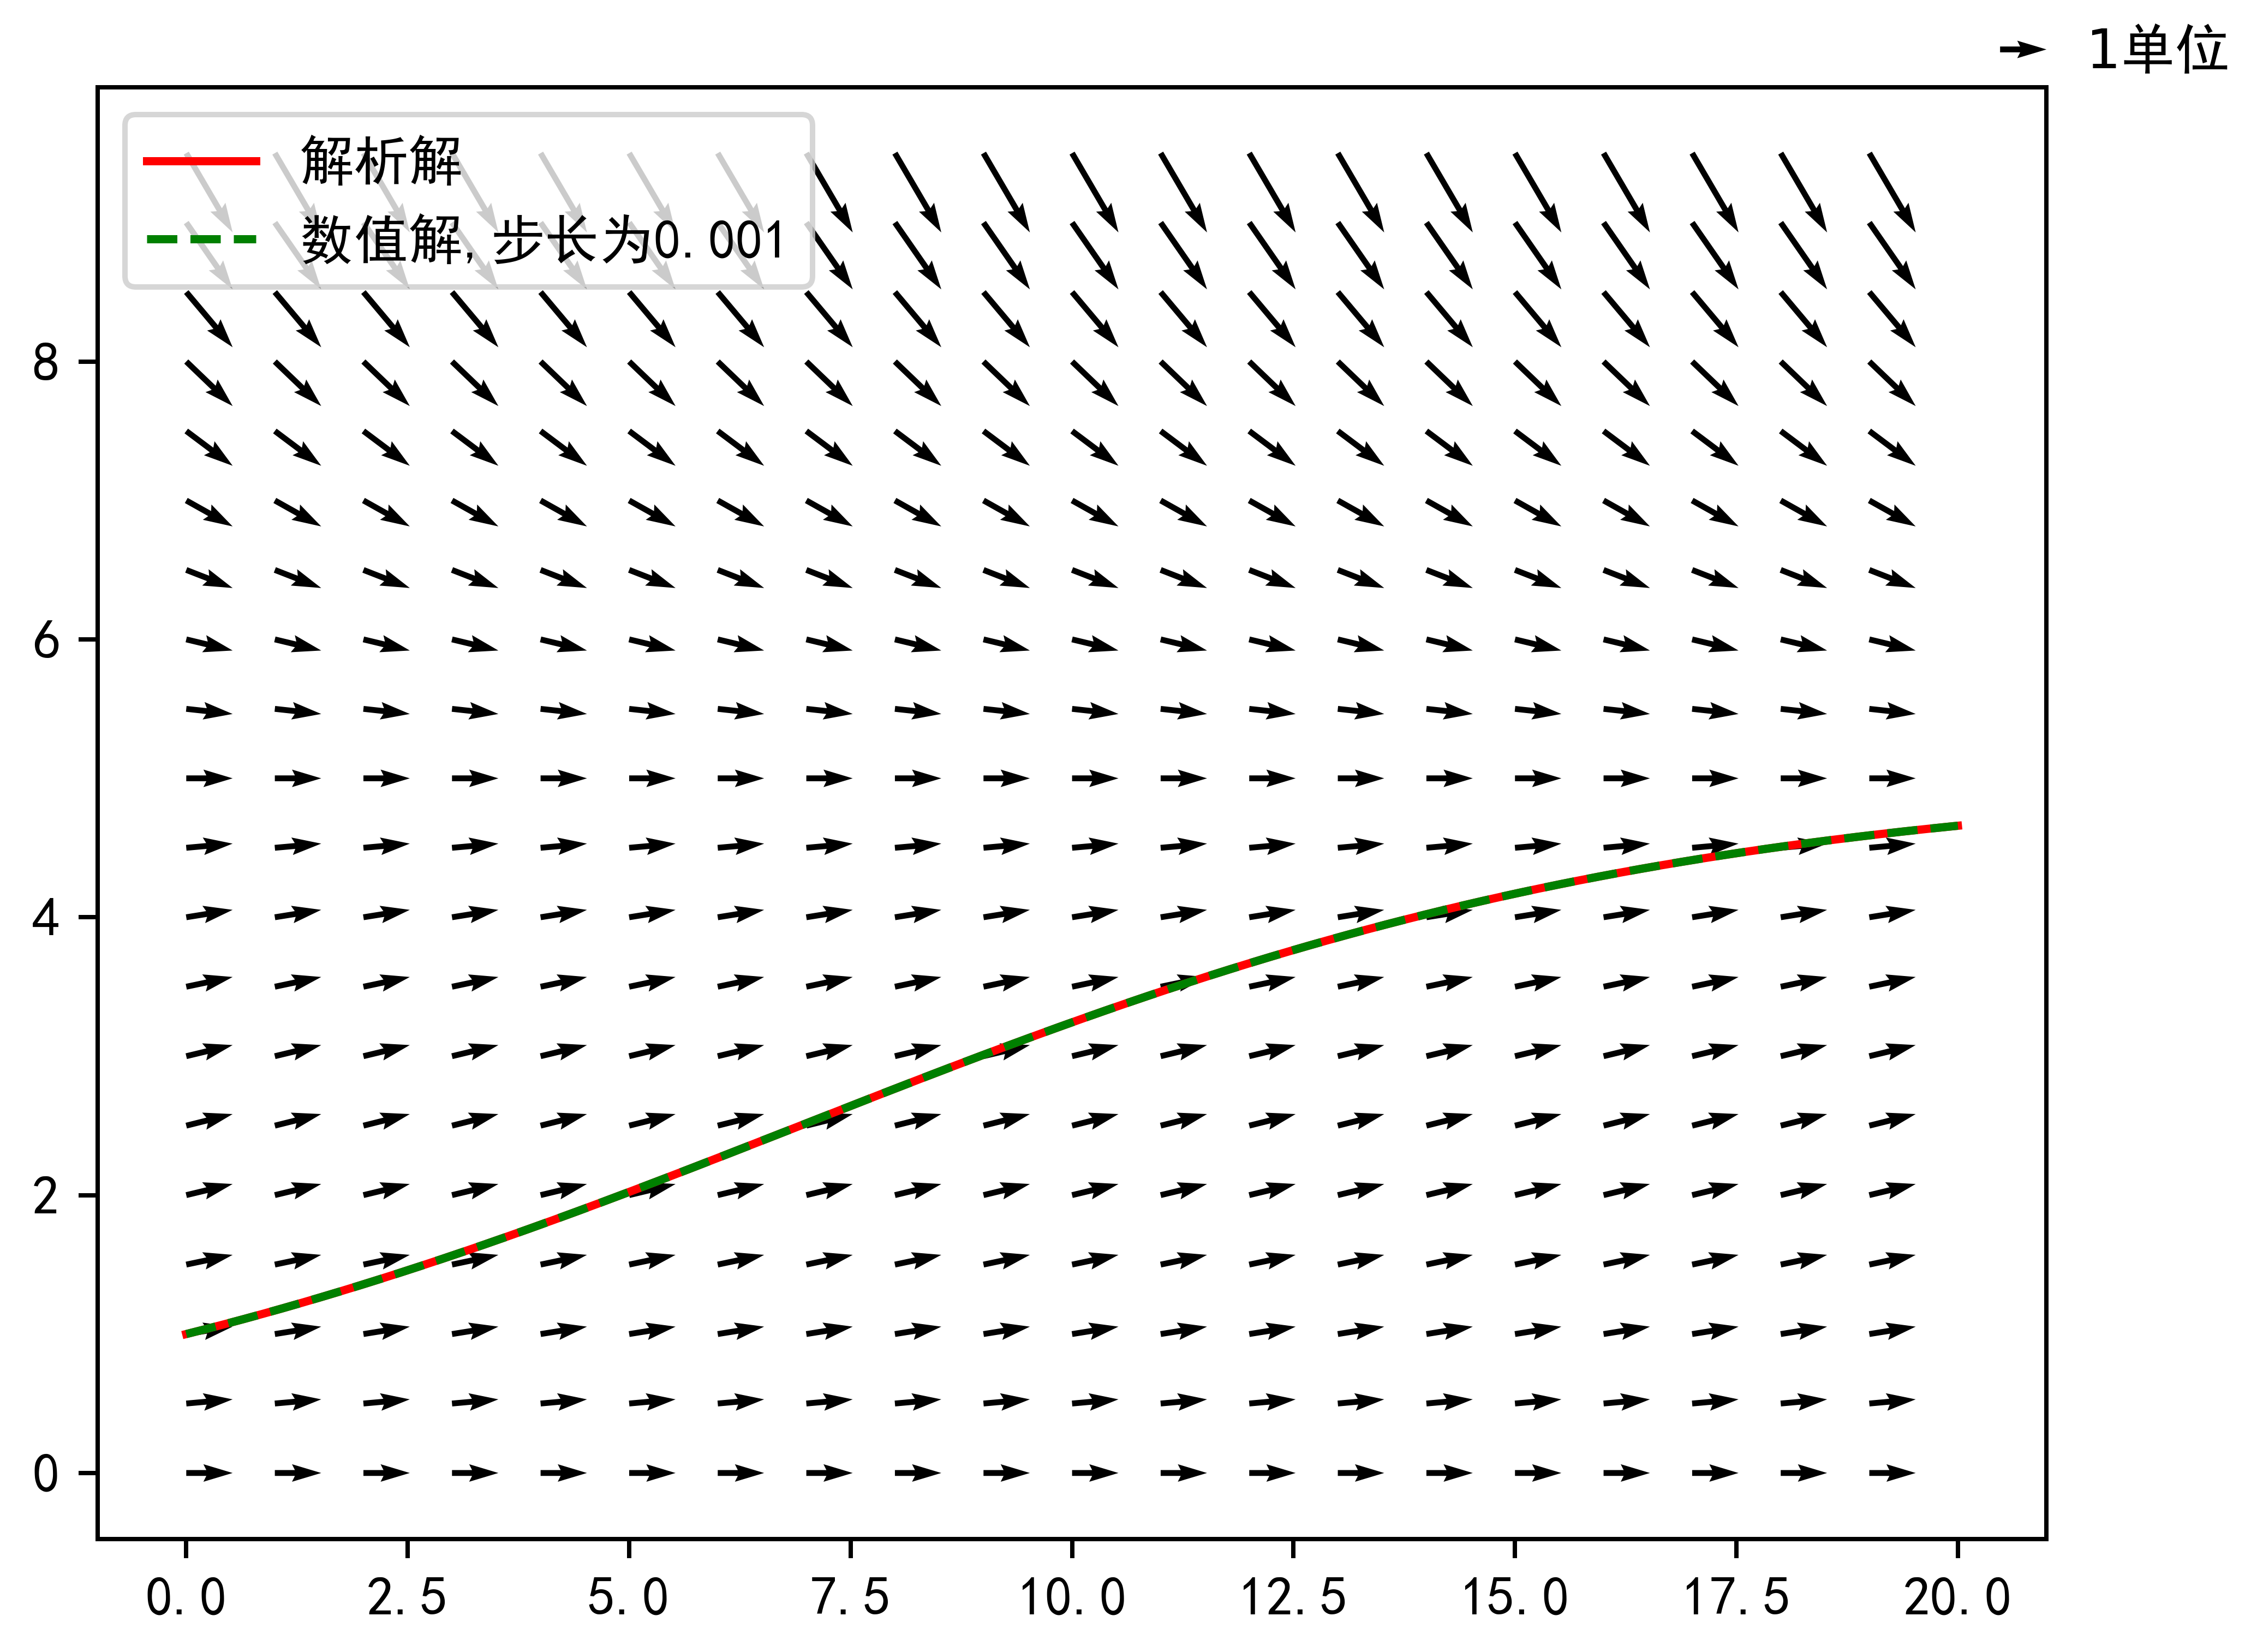
\includegraphics[scale=0.65]{1}
        \caption[图一]{过点$(0,1)$的方程(1)的特解以及方程(1)对应的斜率场}
        \end{figure}
%插入2,过点(0,1)的方程(2)的特解以及方程(2)对应的斜率场
\begin{figure}[H]
        \centering
        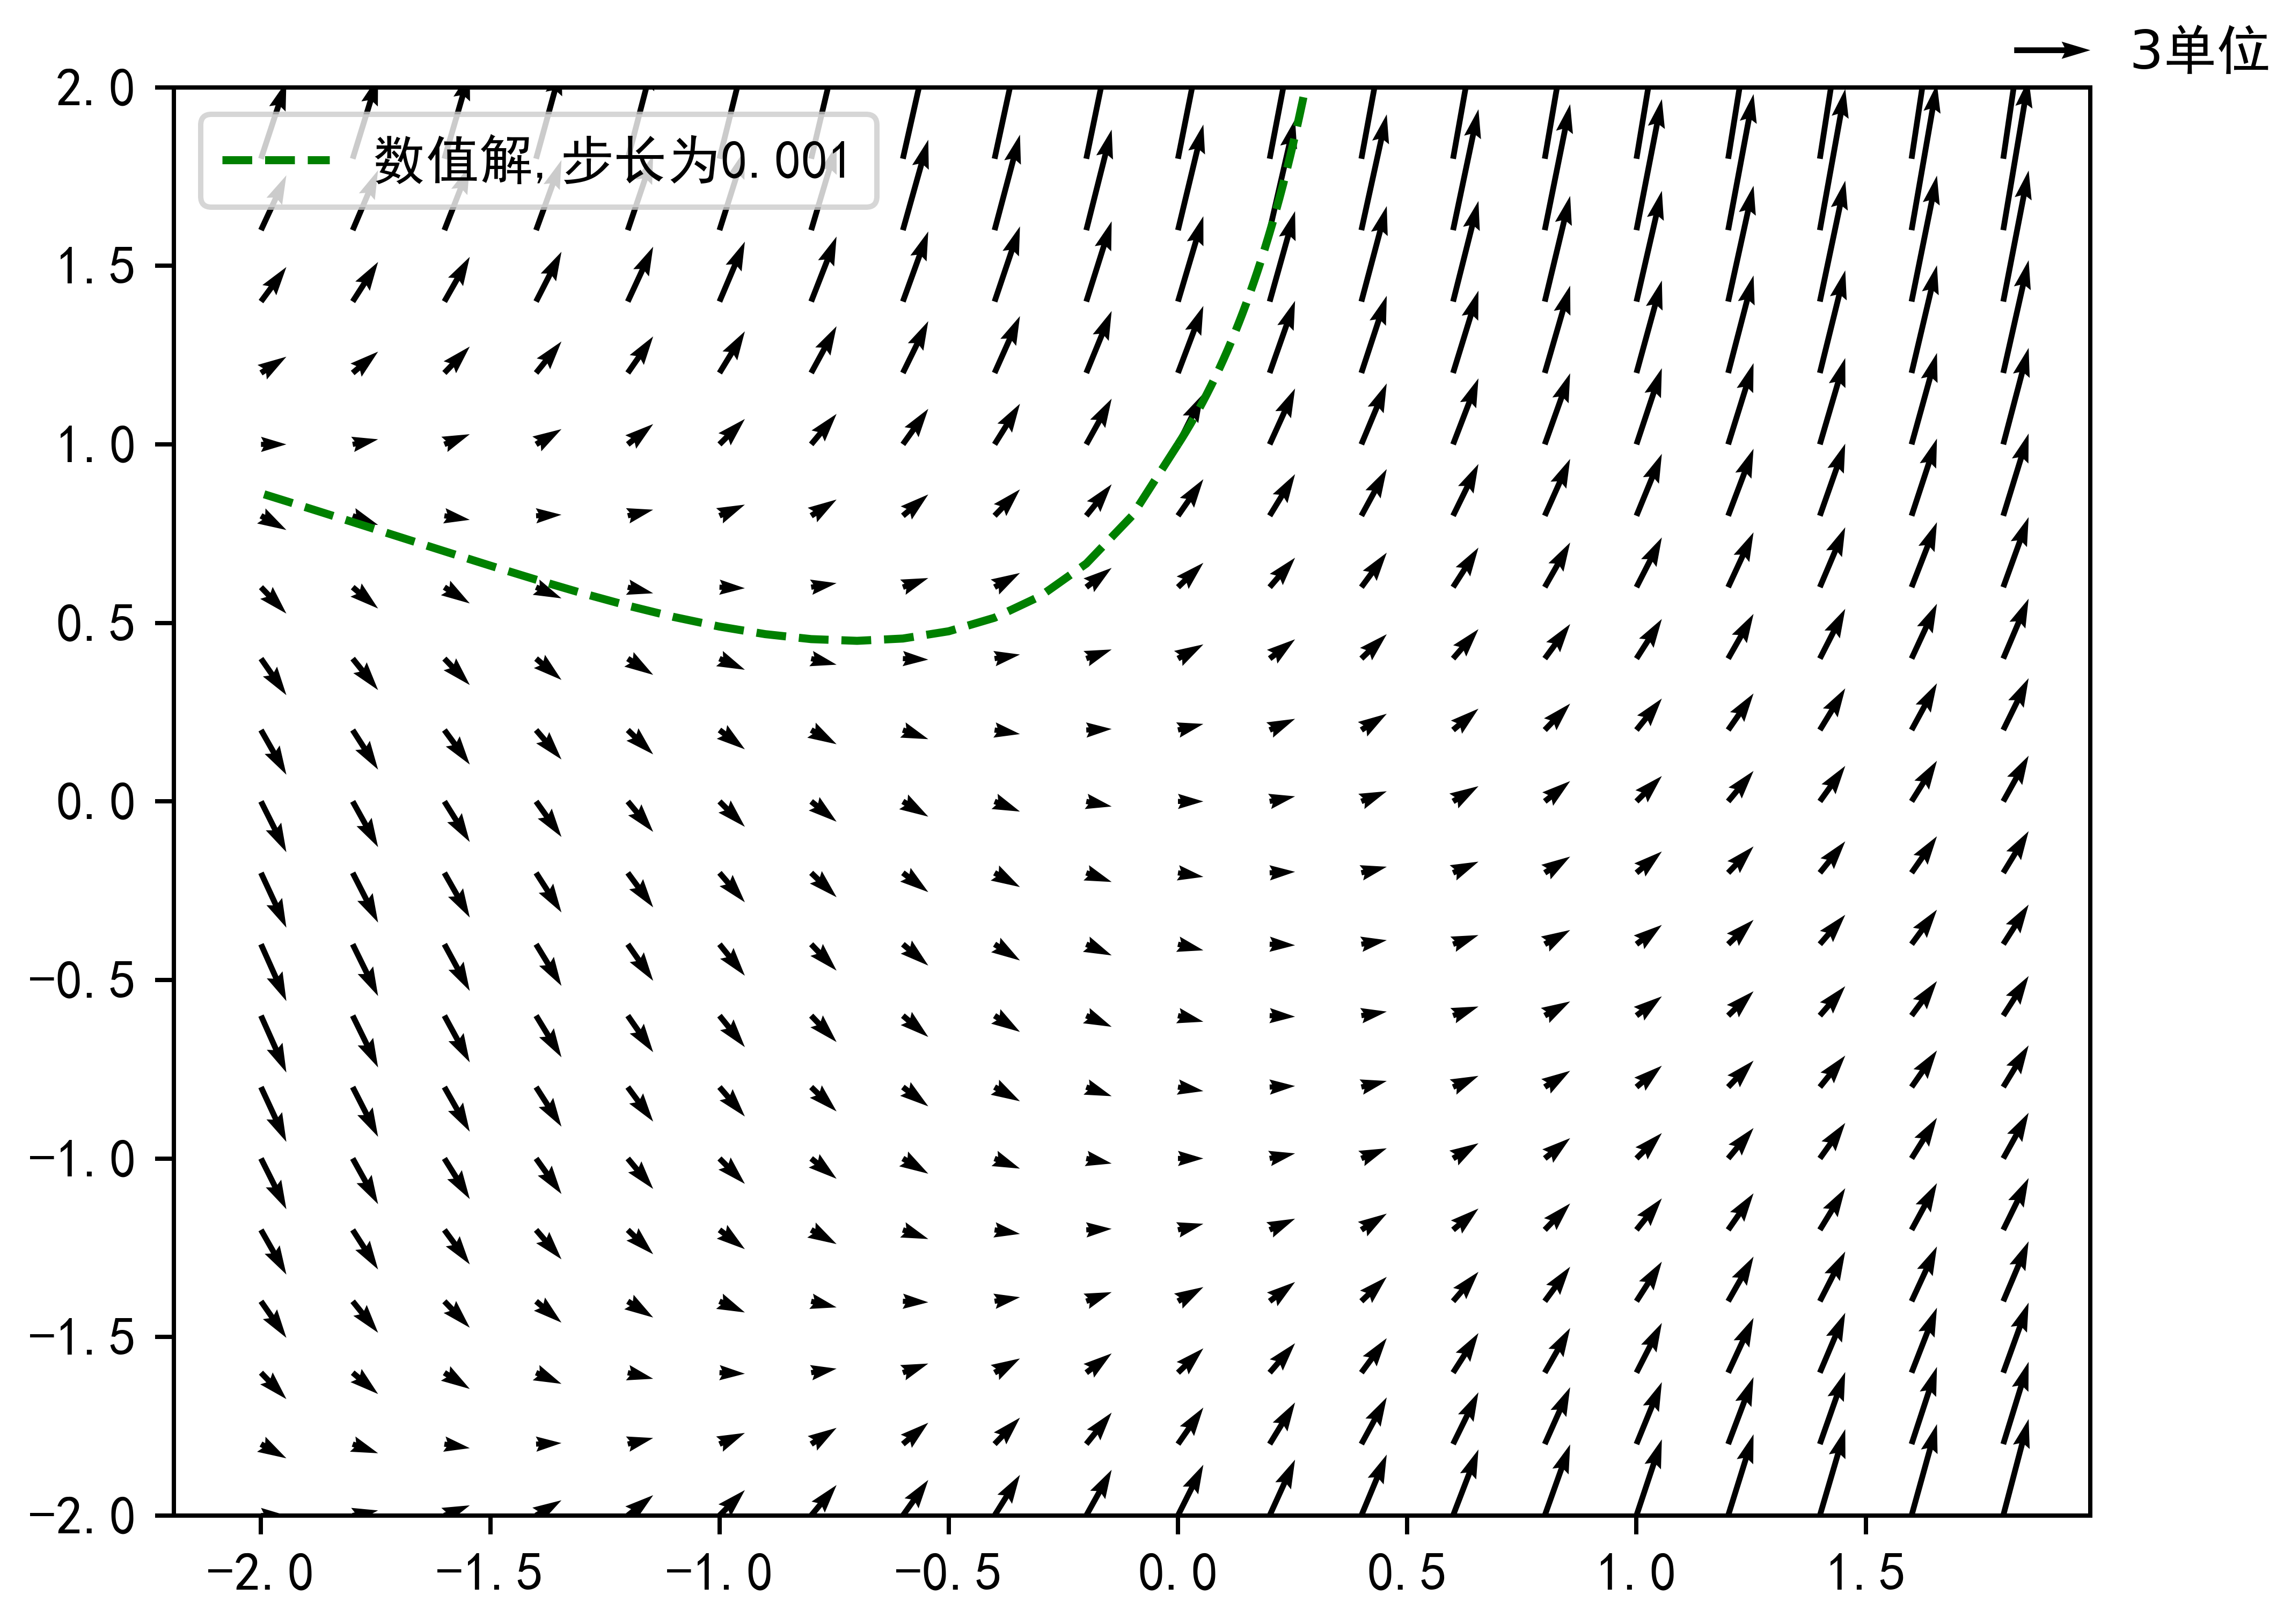
\includegraphics[scale=0.65]{2}
        \caption[图一]{过点$(0,1)$的方程(2)的特解以及方程(2)对应的斜率场}
        \end{figure}
\section{仿照欧拉折线法求解微分方程组的近似解}
\subsection{二元微分方程组}
对于二元微分方程组
\begin{equation*}
        \begin{cases}
    \frac{dx}{dt}=F_1(x,y),\\
    \frac{dy}{dt}=F_2(x,y),
        \end{cases}
    \end{equation*}
%前面要用大括号括起来
可以仿照欧拉折线法来求其过点$(x_0,y_0)$的特解.下面展示的是相应的代码.
%插入展示代码二
\begin{verbatim}
    h,a,b = step length,0,t_0
    # 求解步长和区间端点值
    t = np.arange(a, b+h, h)
    # 在求解区间内间隔 h 取点作为 t 数组
    x,y = np.zeros(t.shape),np.zeros(t.shape)
    # 定义和 t 形状相同的数组存贮数值解的值
    x[0],y[0] = x_0,=y_0
    # 设置初始值
    for i in range( len(t) - 1 ):
        x[i+1]=x[i]+F_1(x[i],y[i])*h
        y[i+1]=y[i]+F_2(x[i],y[i])*h
    #求解
\end{verbatim}


用以上代码求解微分方程组
\begin{equation*}
        \begin{cases}
    \frac{dx}{dt}=0.1x-0.01xy,\\
    \frac{dy}{dt}=-0.05y+0.2xy.\\
    \end{cases}
    \end{equation*}
%前面要用大括号括起来


令步长$h=0.001$并将$(x(t),y(t))$视为平面上的曲线,可得图3-6.
%插入文件夹二中的4张图片,位置应该和起始点在坐标轴上的位置一样,标题即为文件名
\begin{figure}[H]
    \begin{minipage}{0.48\linewidth}
    \centering
    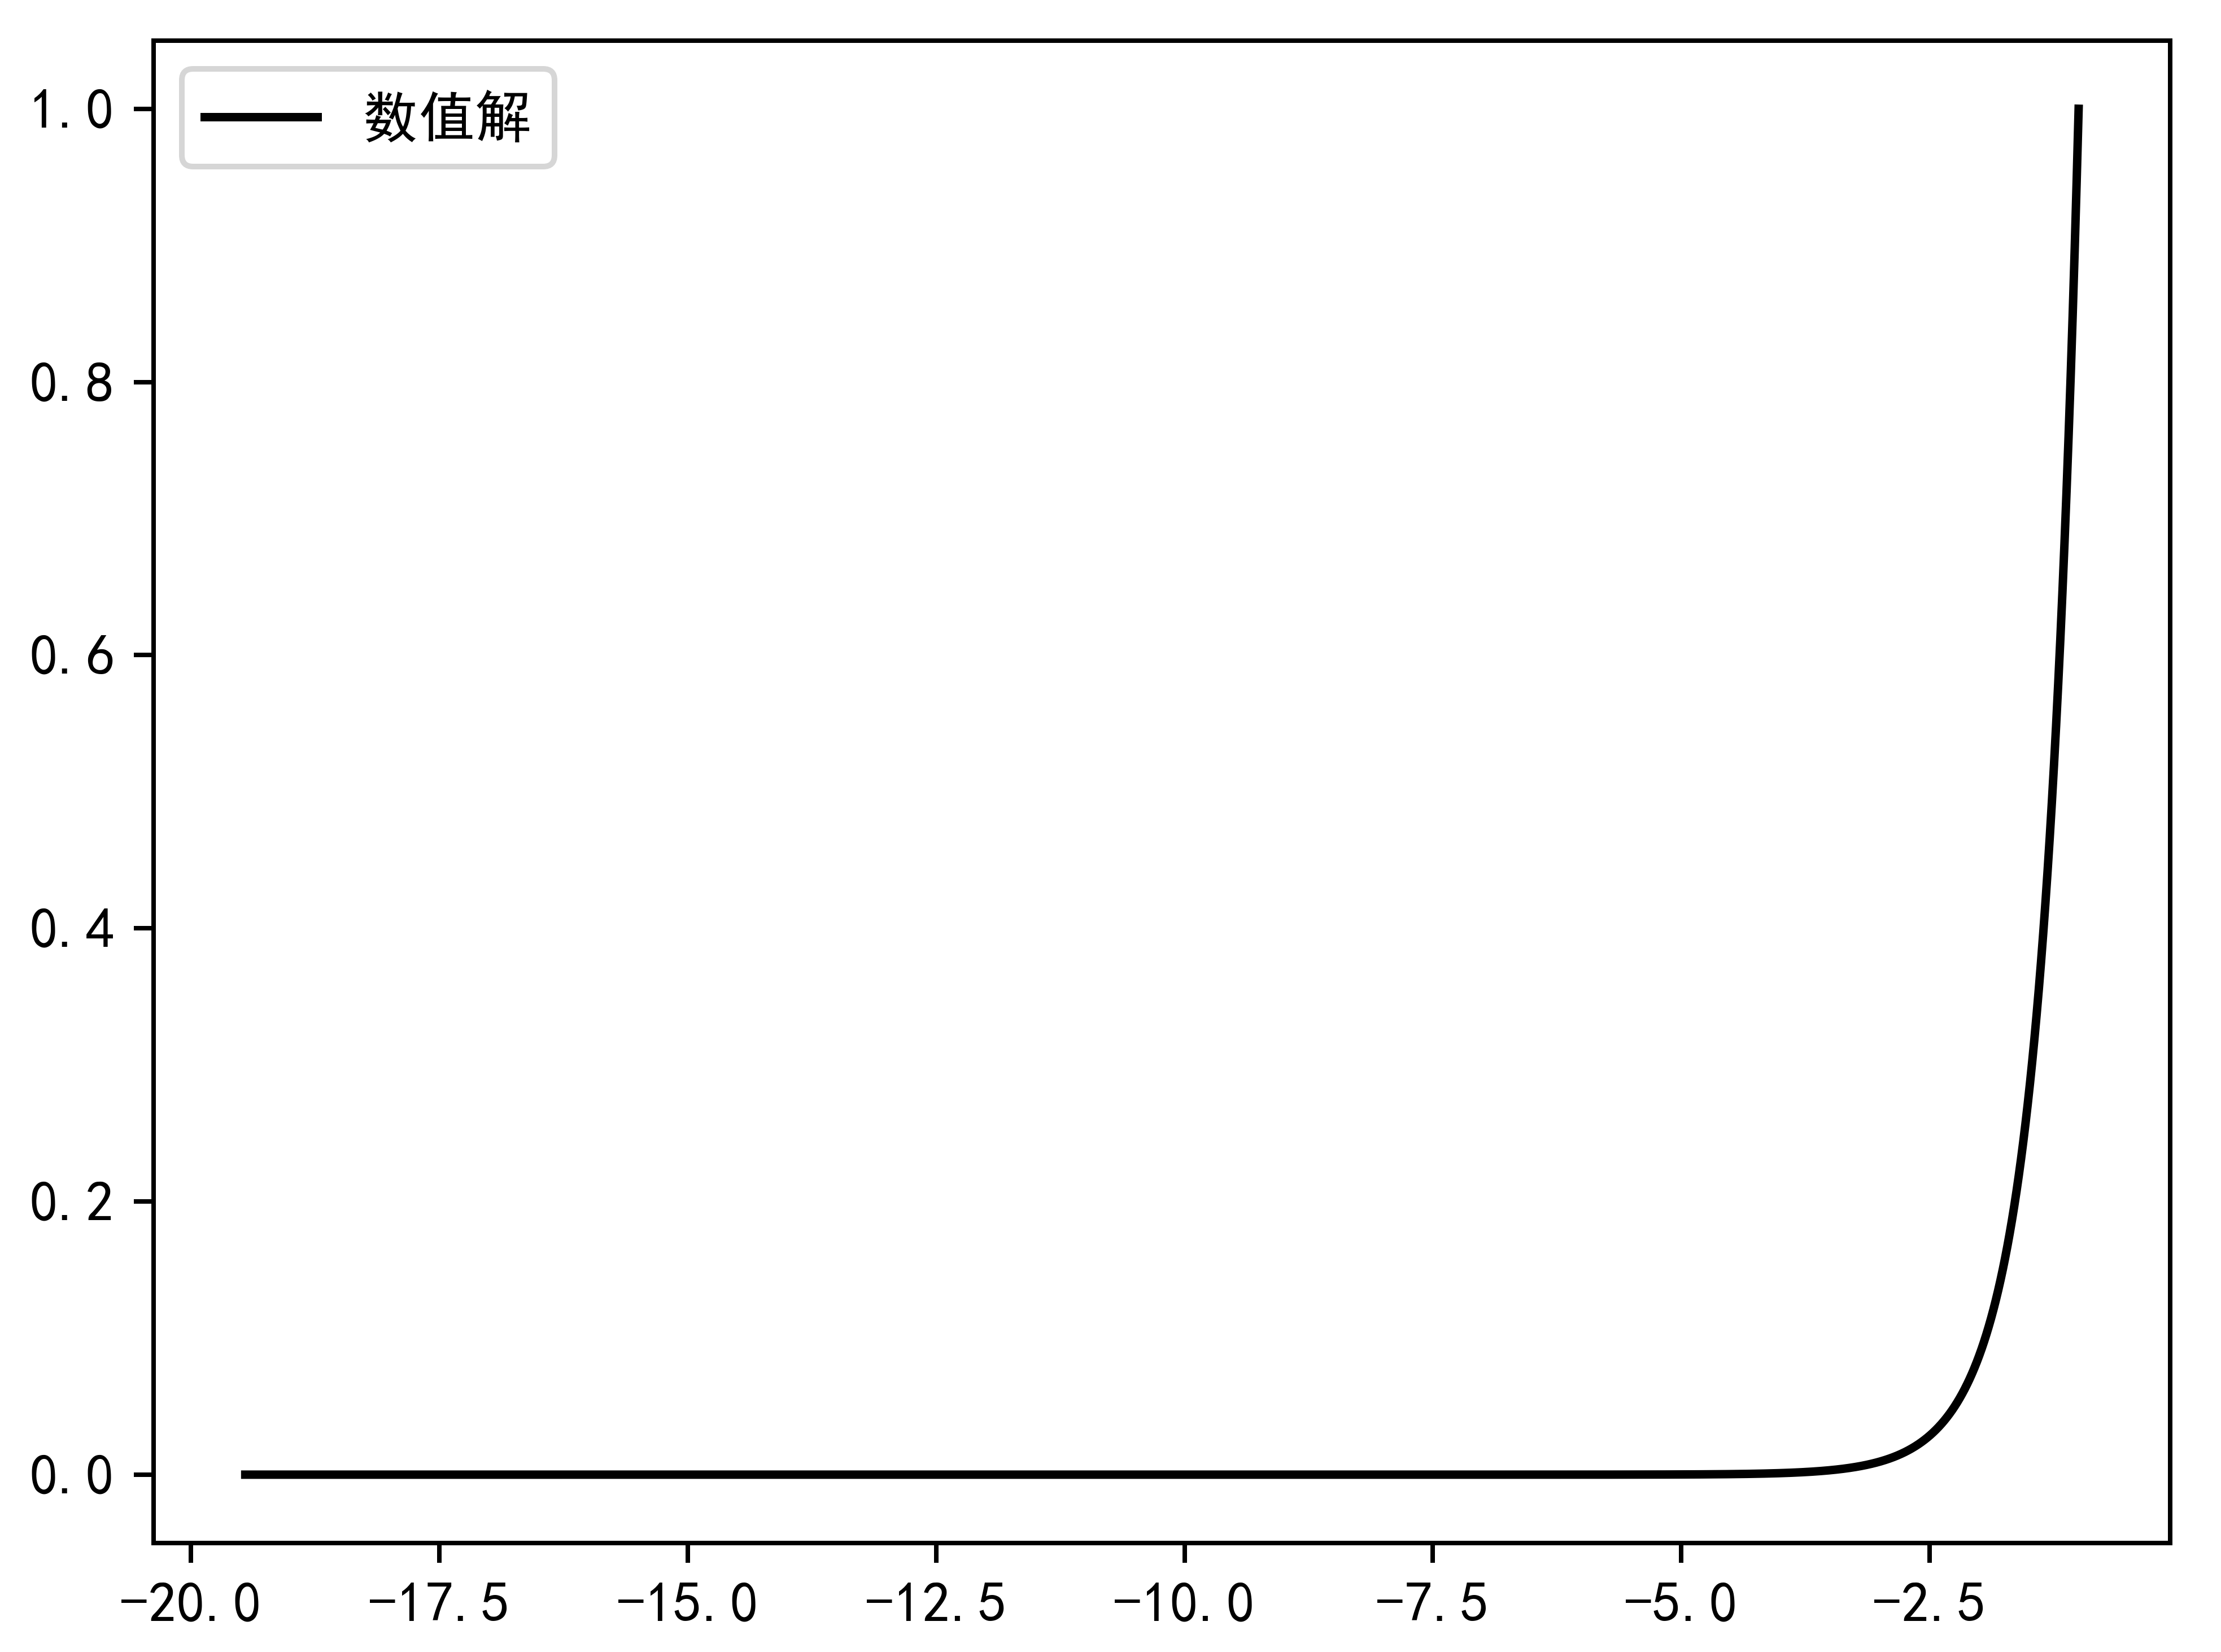
\includegraphics[scale=0.5]{起始点为(-1,1)}
    \caption{起始点为(-1,1)}
    \end{minipage}
    \begin{minipage}{0.48\linewidth}
    \centering
    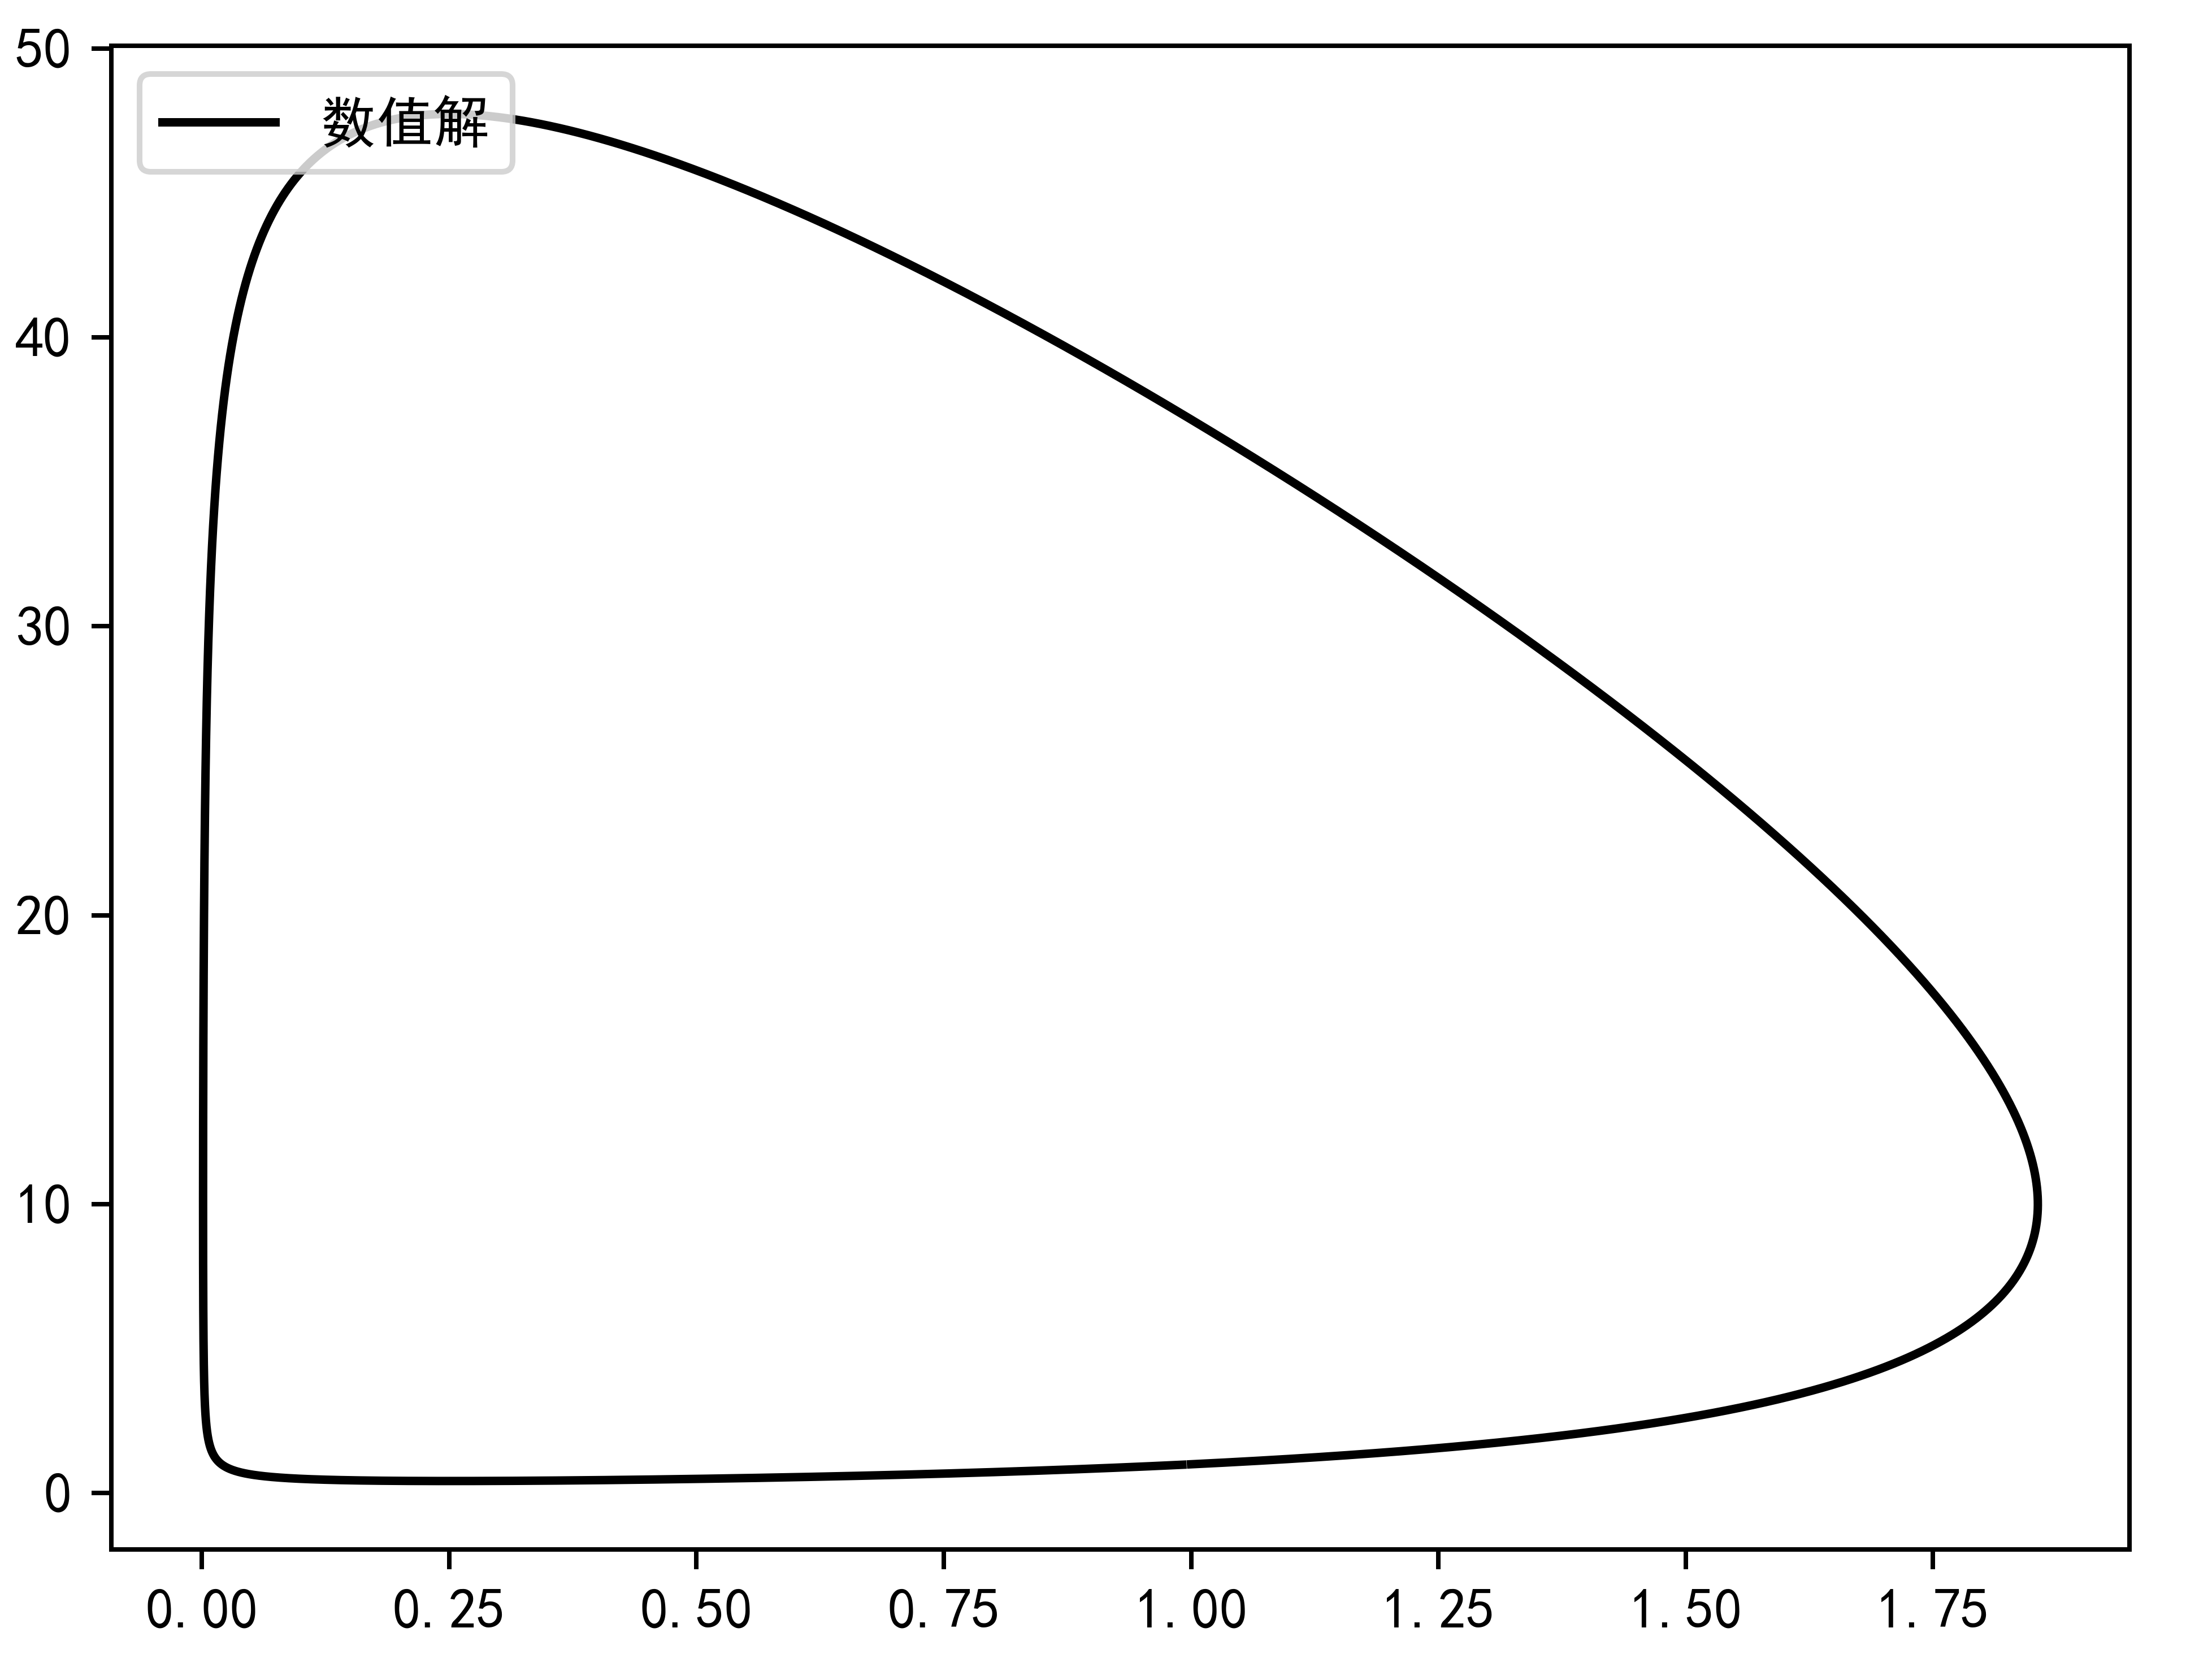
\includegraphics[scale=0.5]{起始点为(1,1)}
    \caption{起始点为(1,1)}
    \end{minipage}
    \end{figure}
\begin{figure}
    \begin{minipage}{0.48\linewidth}
    \centering
    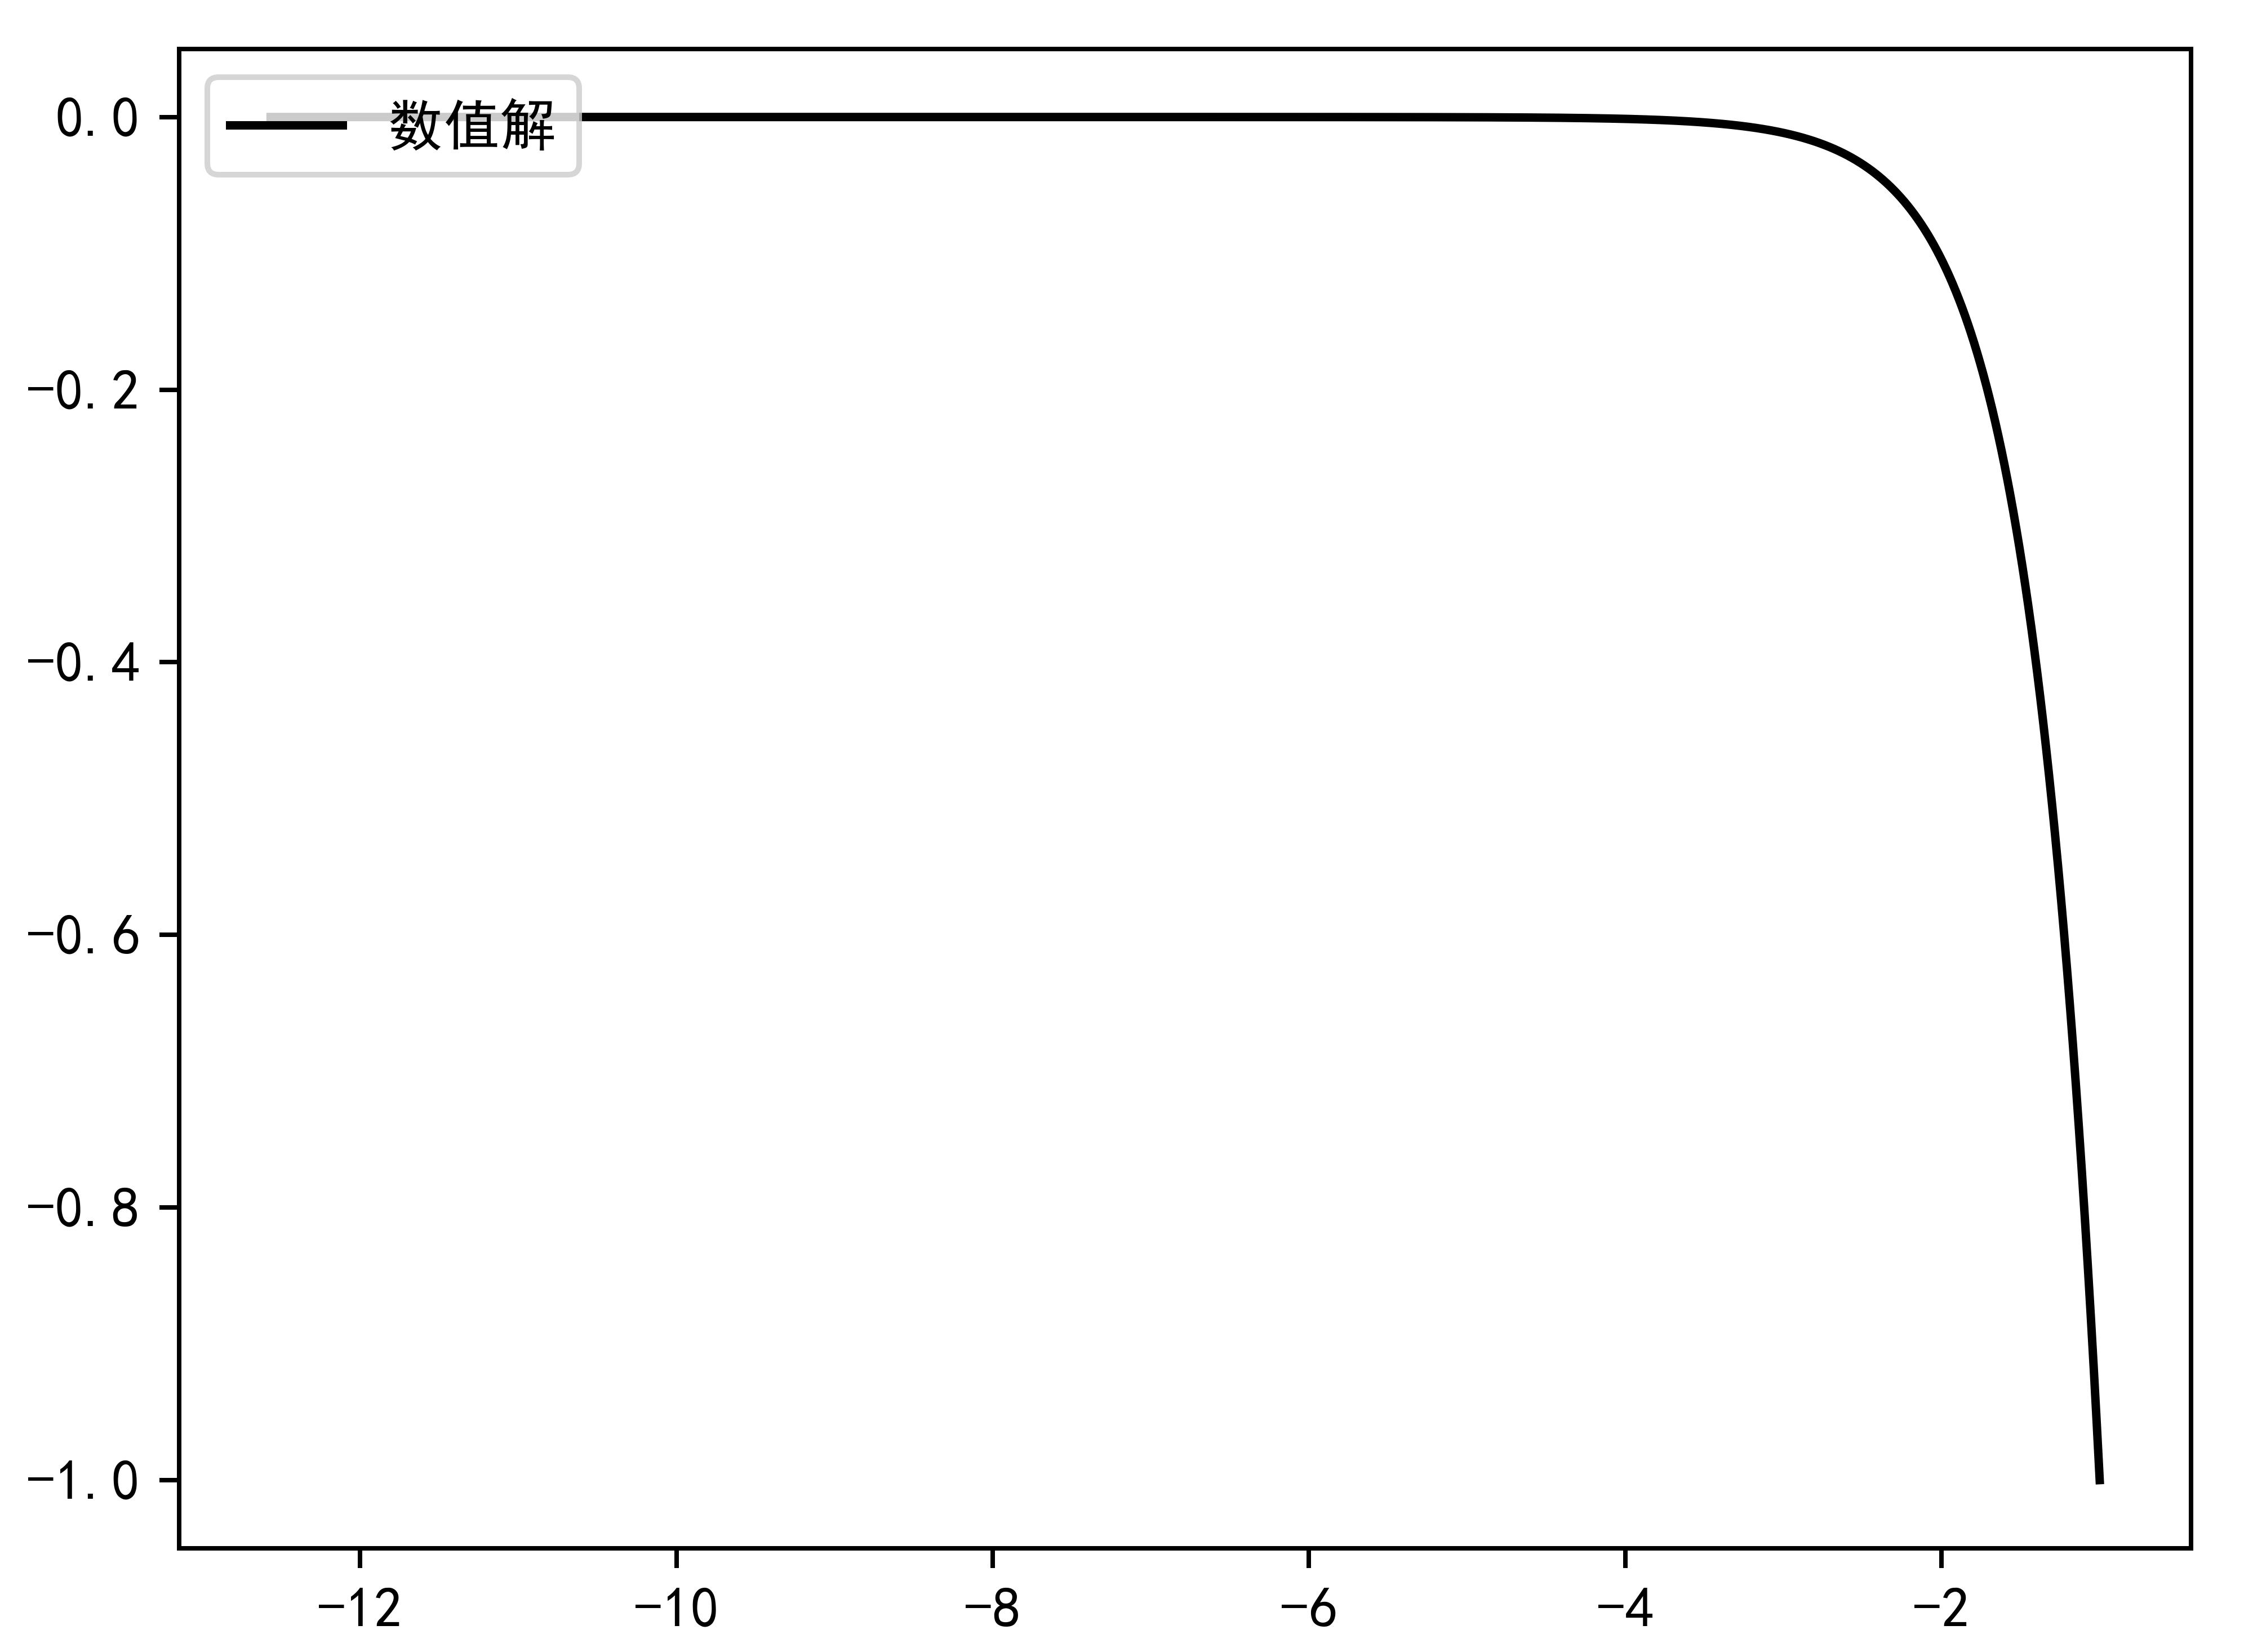
\includegraphics[scale=0.5]{起始点为(-1,-1)}
    \caption{起始点为(-1,-1)}
    \end{minipage}
    \begin{minipage}{0.48\linewidth}
    \centering
    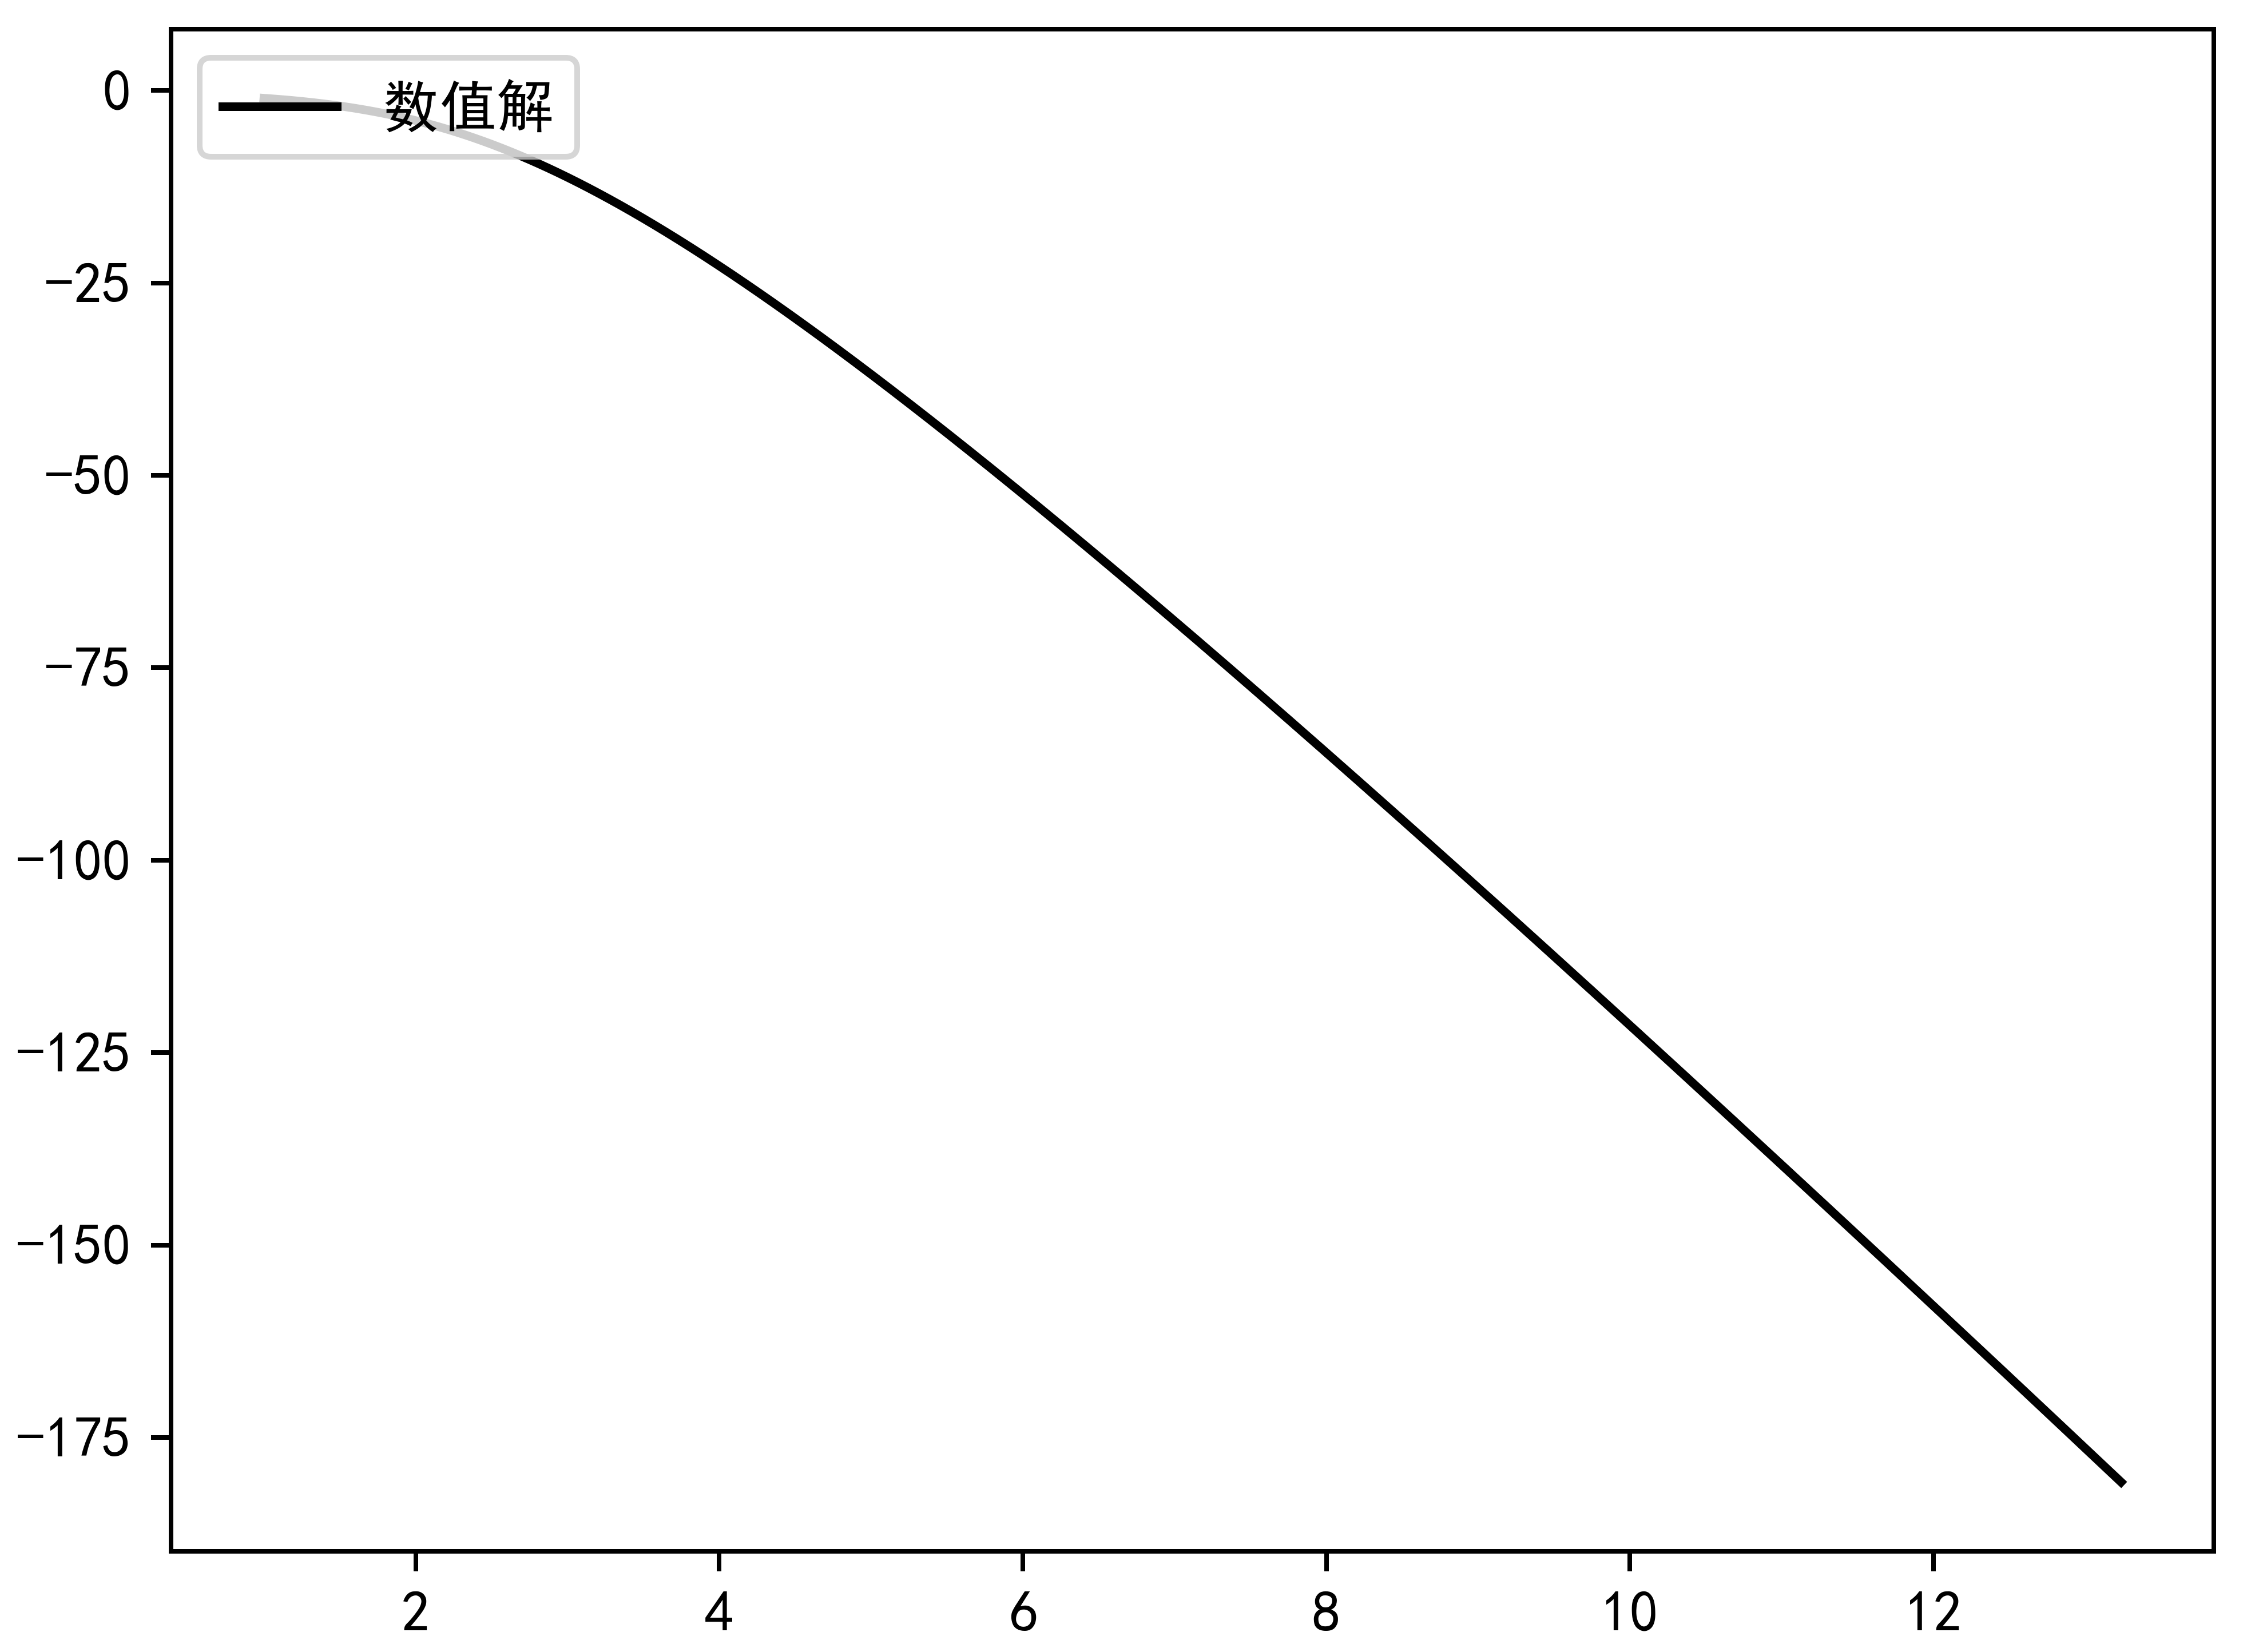
\includegraphics[scale=0.5]{起始点为(1,-1)}
    \caption{起始点为(1,-1)}
    \end{minipage}
\end{figure}

\subsection{三元微分方程组}
对于三元微分方程组

\begin{equation*}
        \begin{cases}
\frac{dx}{dt}=F_1(x,y,z),\\
\frac{dy}{dt}=F_2(x,y,z),\\
\frac{dz}{dt}=F_3(x,y,z),\\
\end{cases}
\end{equation*}
%前面要用大括号括起来
可以仿照欧拉折线法来求其过点$(x_0,y_0,z_0)$的特解.下面展示的是相应的代码.
%插入展示代码三
\begin{verbatim}
    h,a,b = step length,0,t_0 
    # 求解步长和区间端点值
    t = np.arange(a, b+h, h)
    # 在求解区间内间隔 h 取点作为 t 数组
    x,y,z = np.zeros(t.shape),np.zeros(t.shape),np.zeros(t.shape)
    # 定义和 t 形状相同的数组存贮数值解的值
    x[0],y[0],z[0] = x_0,y_0,z_0
    # 设置初始值
    for i in range( len(t) - 1 ):
        x[i+1]=x[i]+F_1(x[i],y[i],z[i])*h
        y[i+1]=y[i]+F_2(x[i],y[i],z[i])*h
        z[i+1]=z[i]+F_3(x[i],y[i],z[i])*h
    #求解
\end{verbatim}


用以上代码求解微分方程组
\begin{equation*}
        \begin{cases}
\frac{dx}{dt}=10(y-x),\\
\frac{dy}{dt}=28x-y-xz,\\
\frac{dz}{dt}=xy-\frac{8}{3}z.\\
\end{cases}
\end{equation*}
%前面要用大括号括起来


将$(x(t),y(t),z(t))$视为空间中的曲线,取若干个起始点以及不同的步长$h$可得以下图像.
%插入文件夹三中的图片,其中每个子文件中有5张,理想排版是占一整页,布局为
%   1   2
%   3   4
%     5
\begin{figure}[h]
    \begin{minipage}{0.48\linewidth}
    \centering
    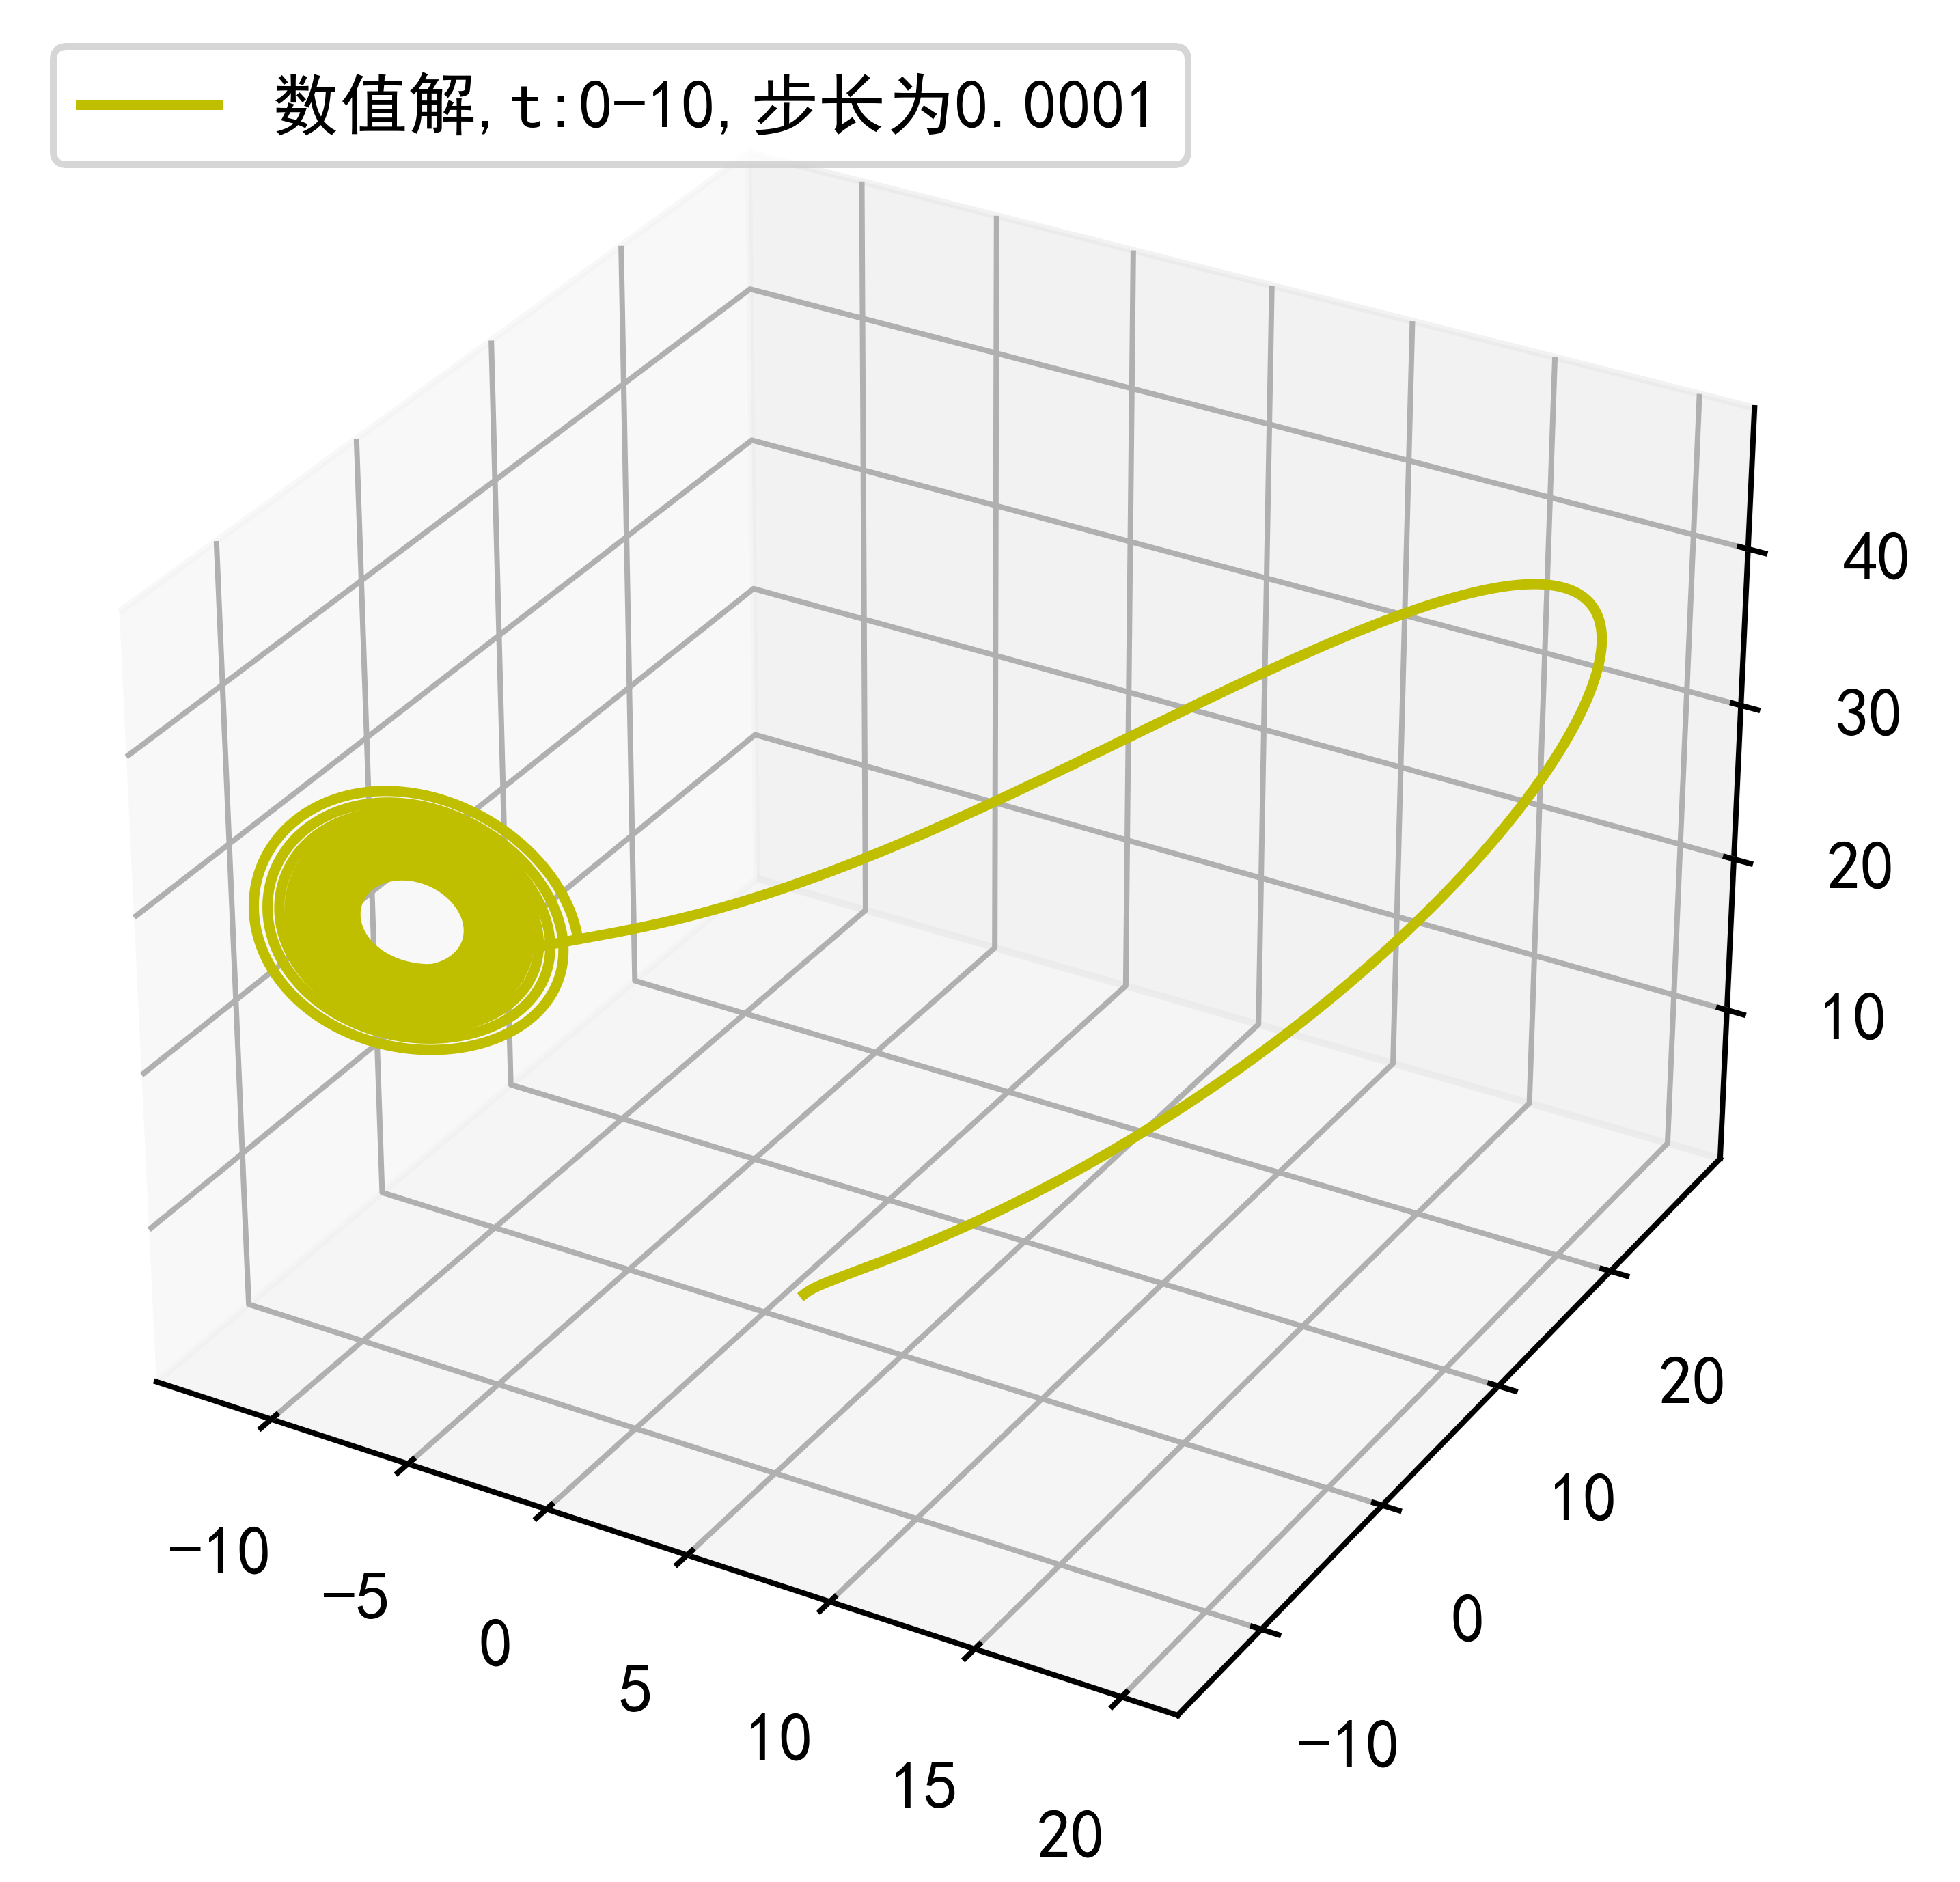
\includegraphics[scale=0.65]{11}
    \caption{起始点为(1,1,1)}
    \end{minipage}
    \begin{minipage}{0.48\linewidth}
    \centering
    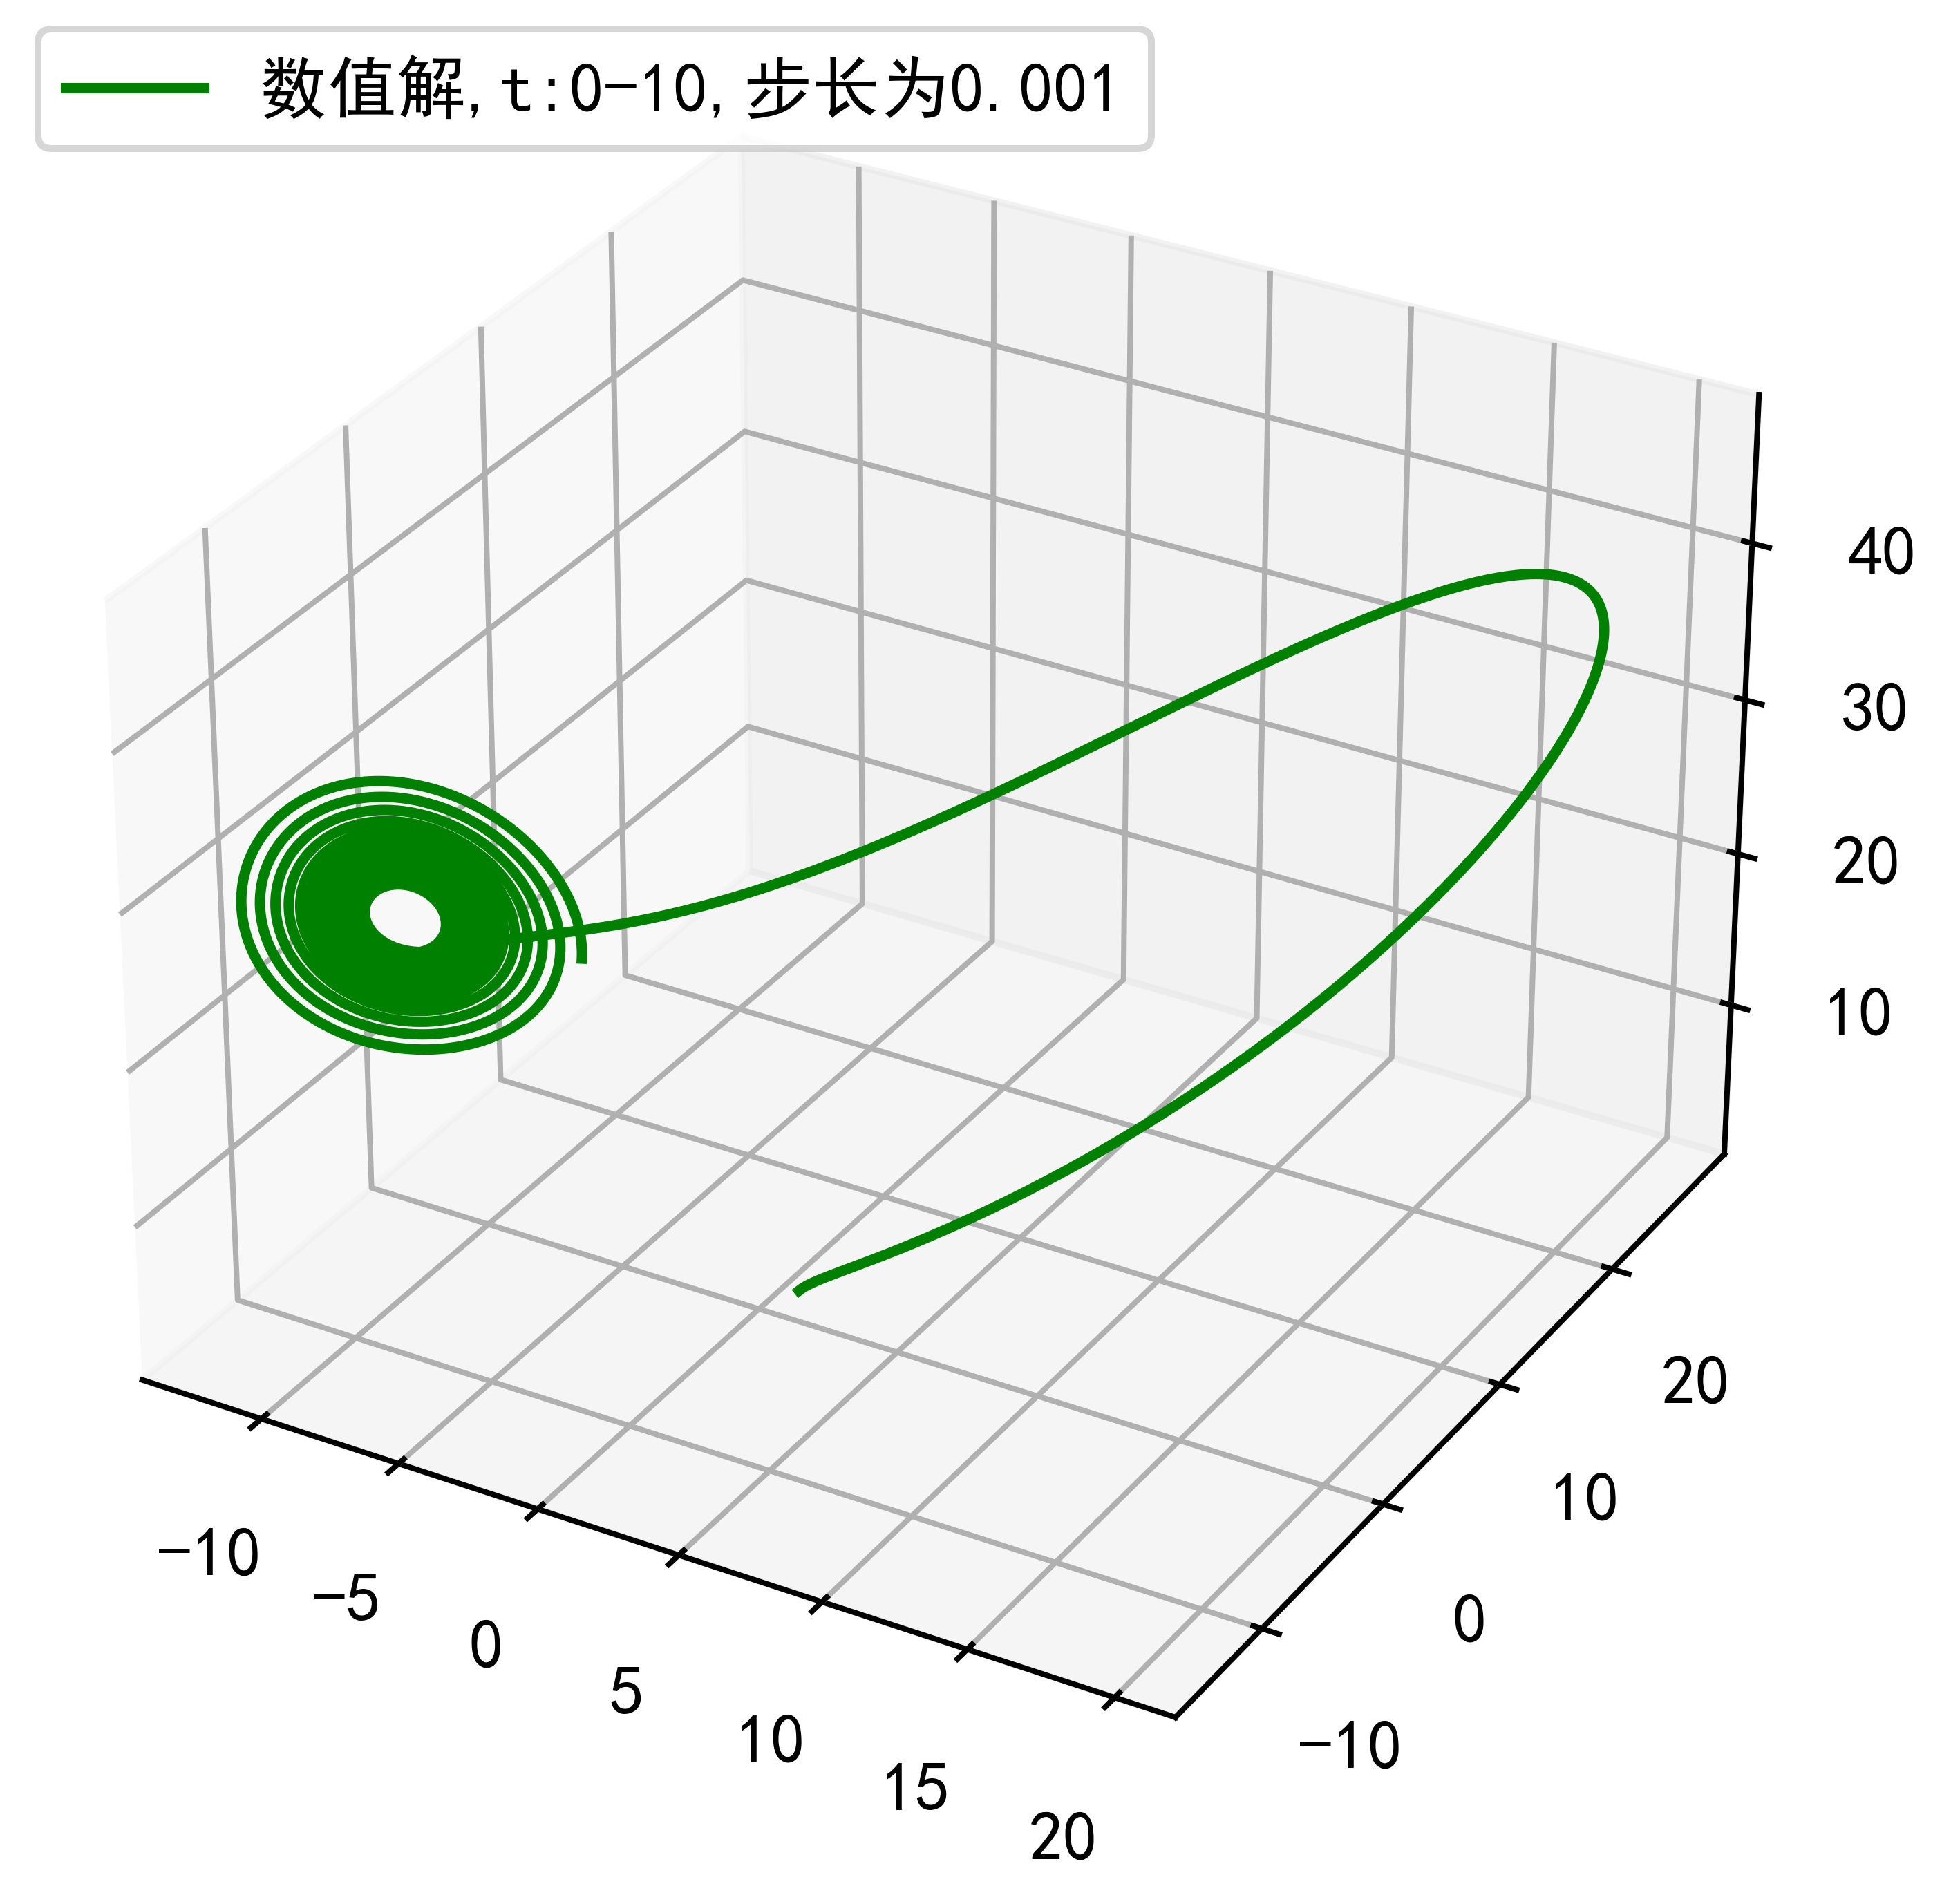
\includegraphics[scale=0.65]{12}
    \caption{起始点为(1,1,1)}
    \end{minipage}
\end{figure}
\begin{figure}[h]
    \begin{minipage}[h]{0.48\linewidth}
    \centering
    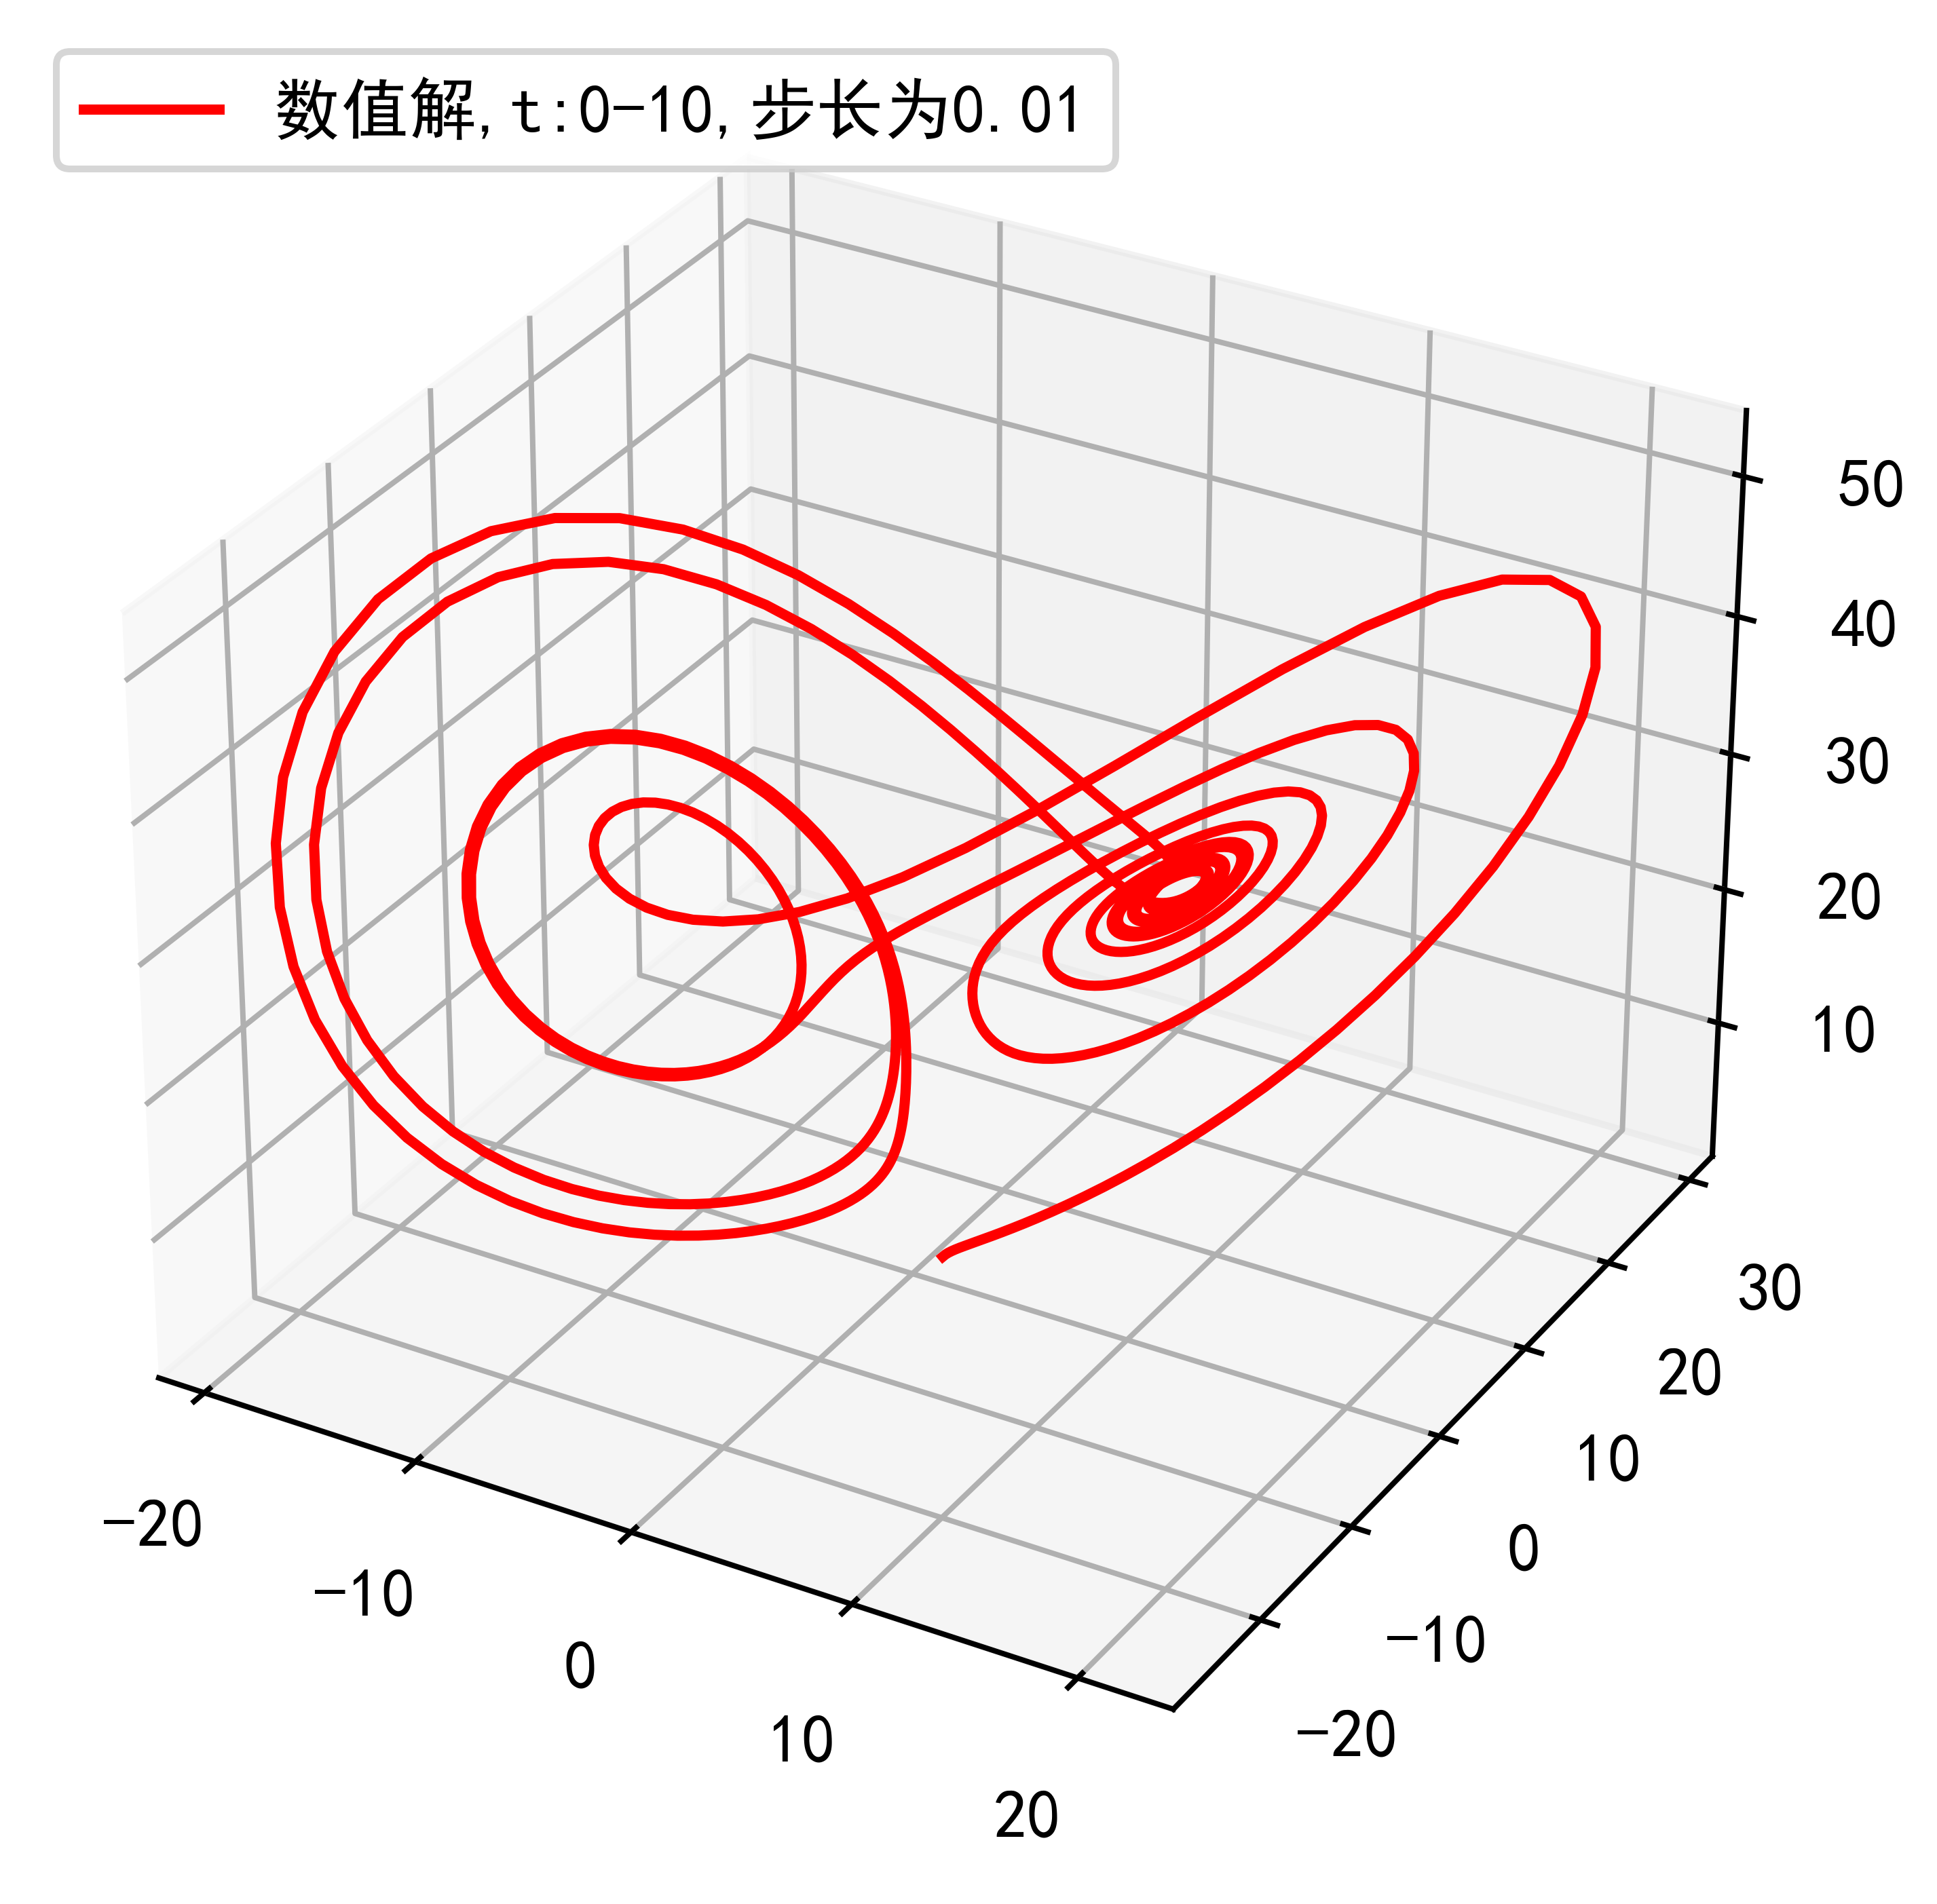
\includegraphics[scale=0.65]{13}
    \caption{起始点为(1,1,1)}
    \end{minipage}
    \begin{minipage}[h]{0.48\linewidth}
    \centering
    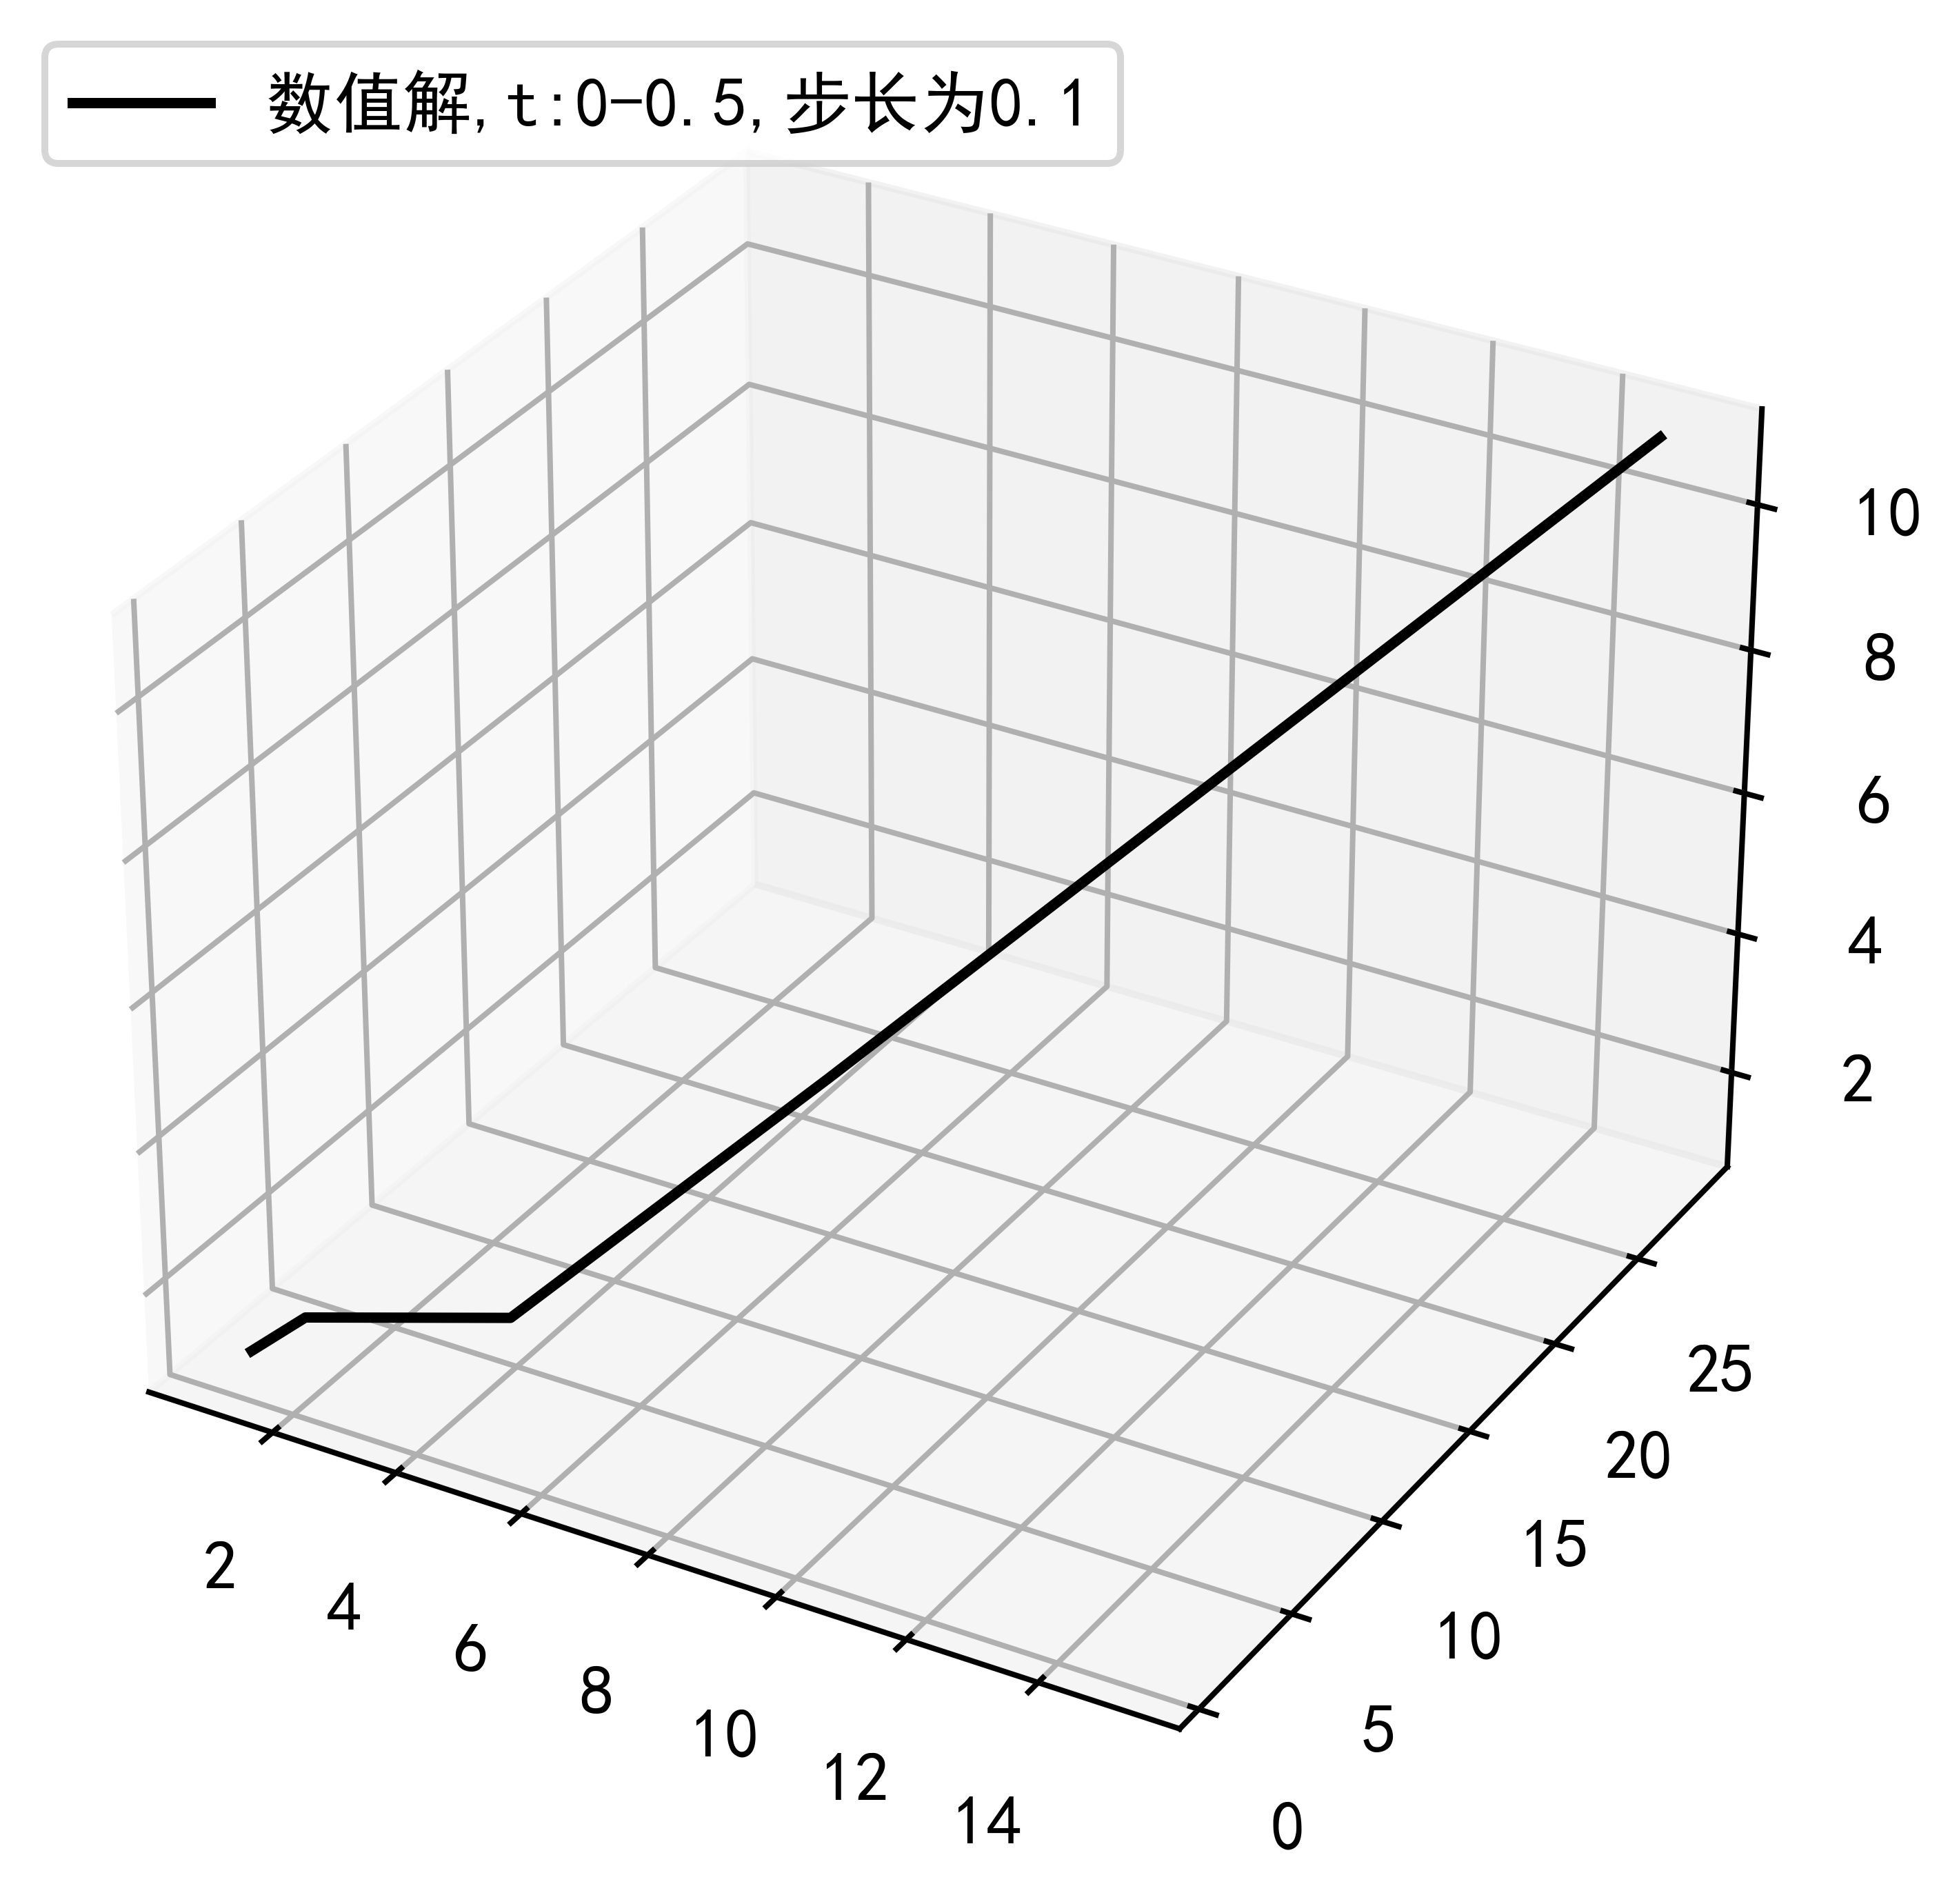
\includegraphics[scale=0.65]{14}
    \caption{起始点为(1,1,1)}
    \end{minipage}
\end{figure}
\begin{figure}[H]
    \centering
    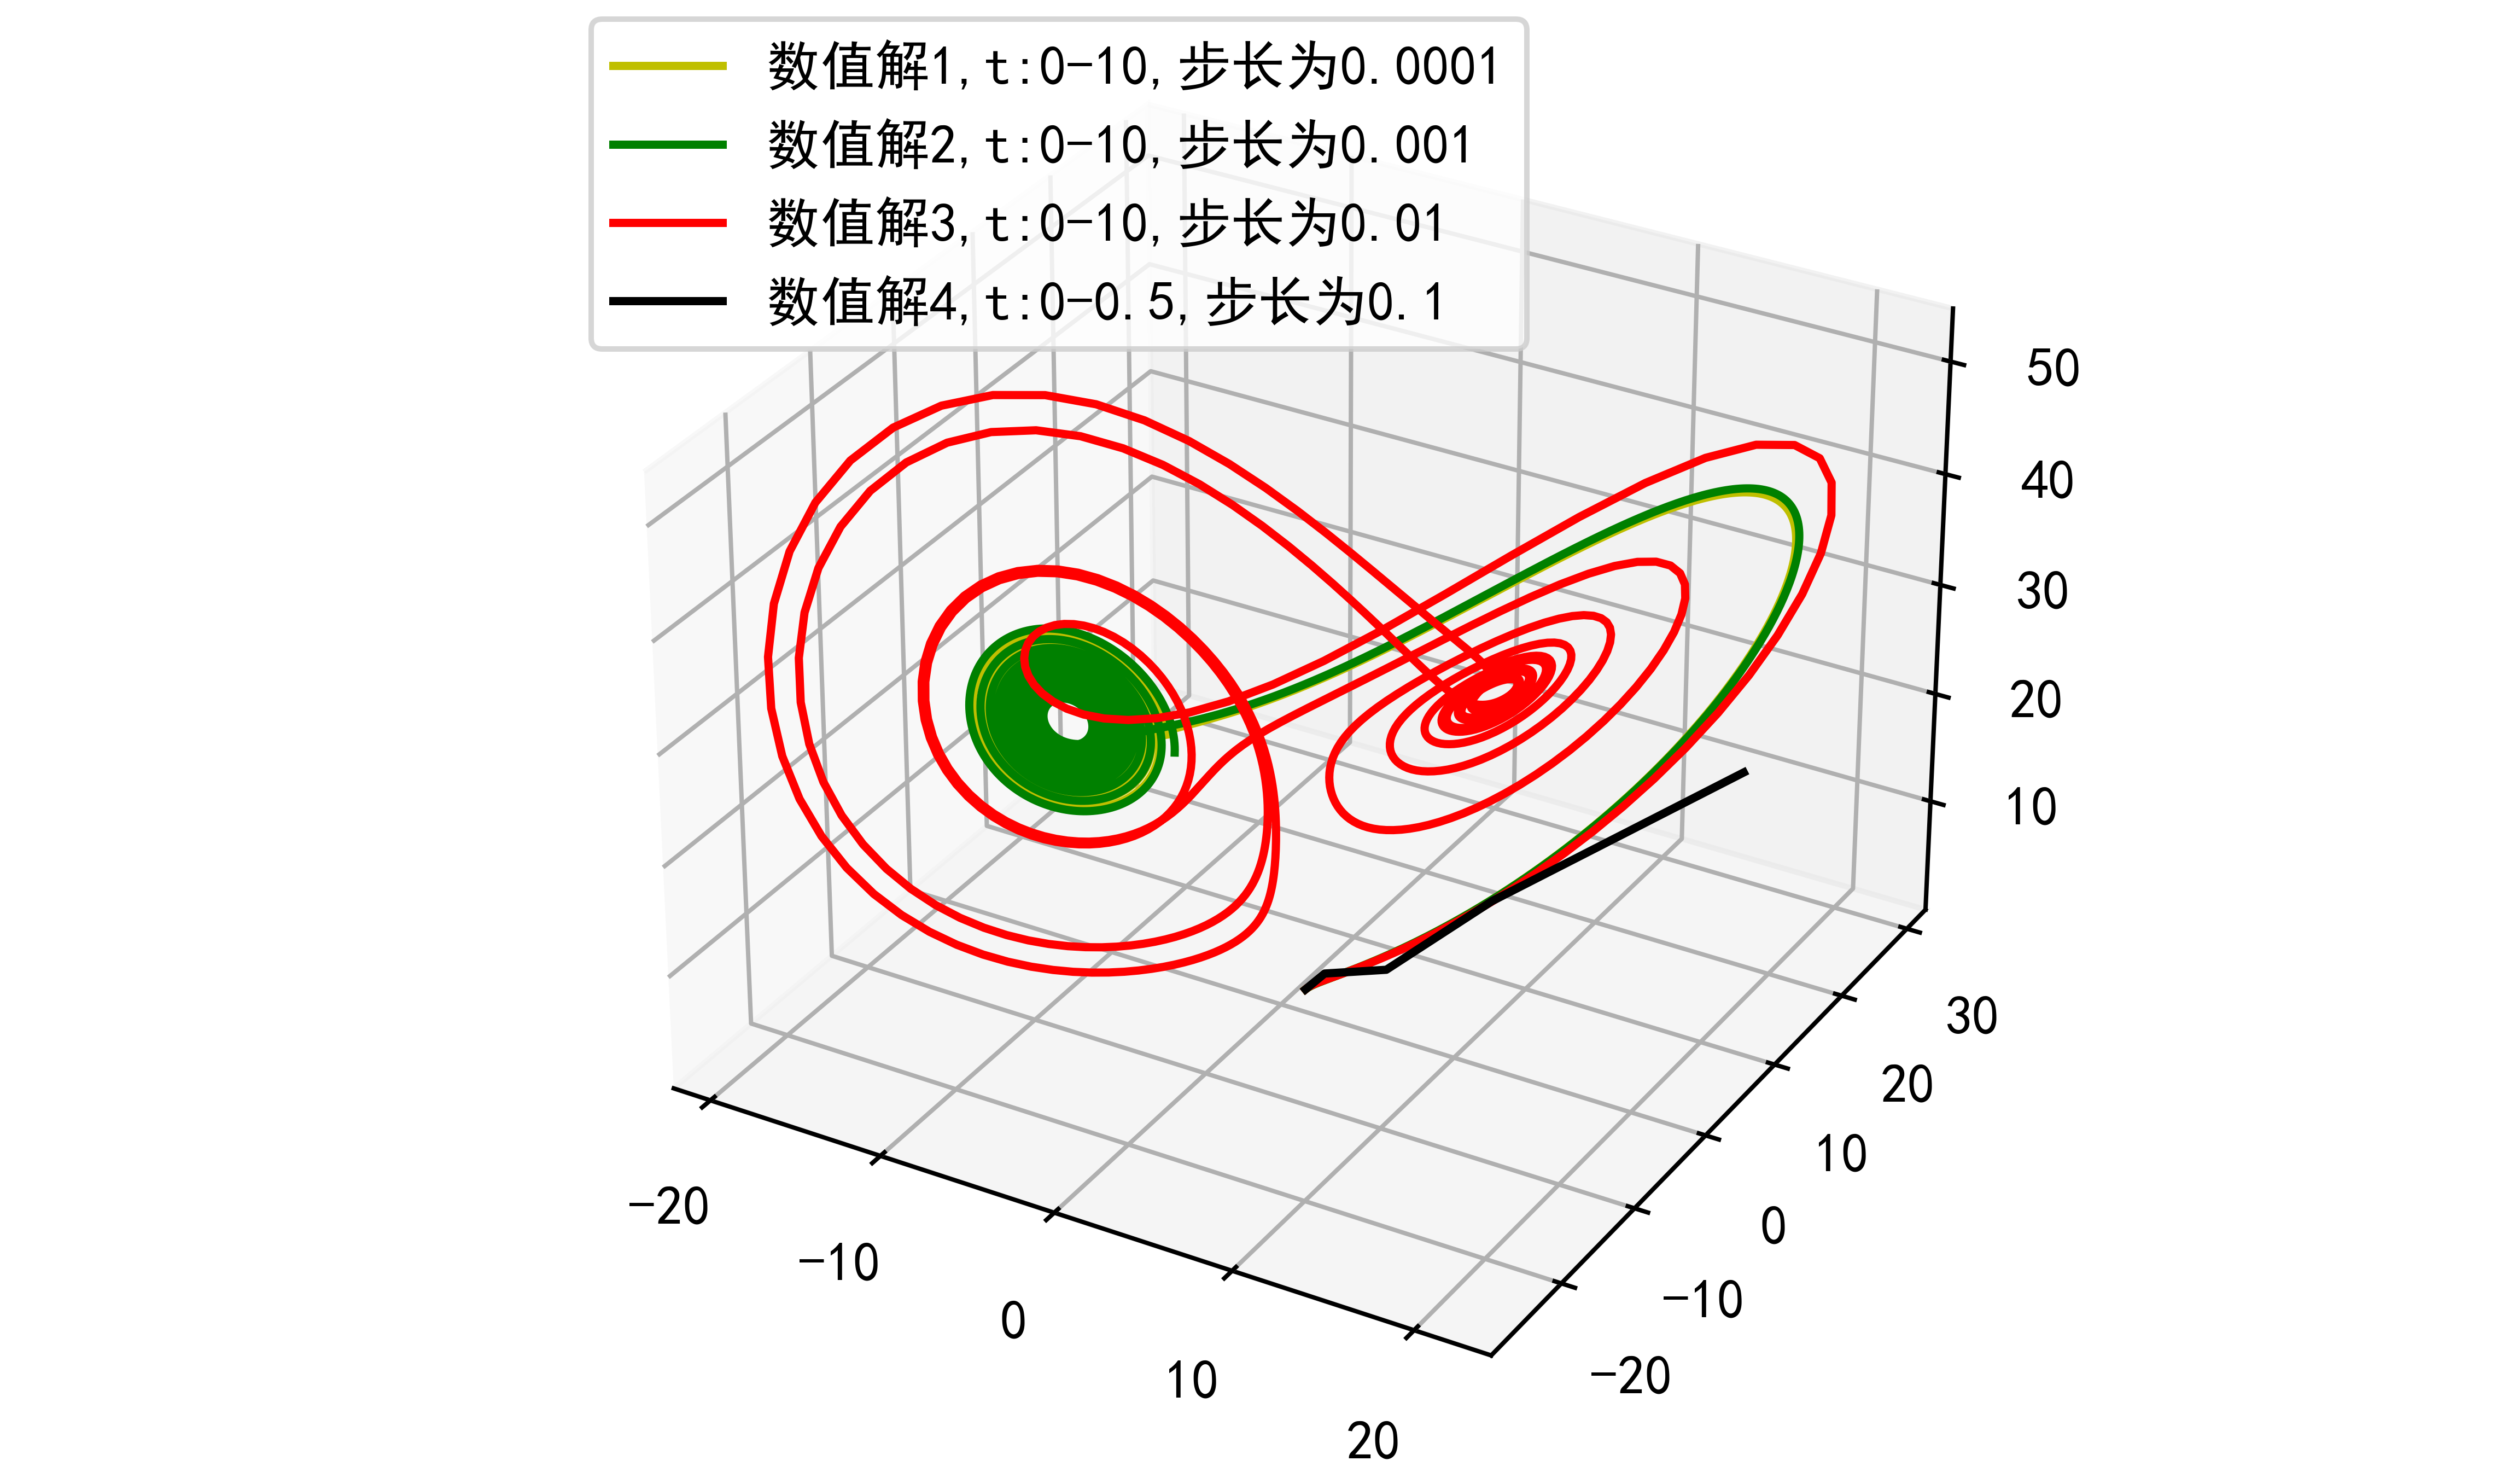
\includegraphics[scale=0.7]{15}
    \caption{起始点为(1,1,1)}
\end{figure}

\begin{figure}[h]
    \begin{minipage}{0.48\linewidth}
    \centering
    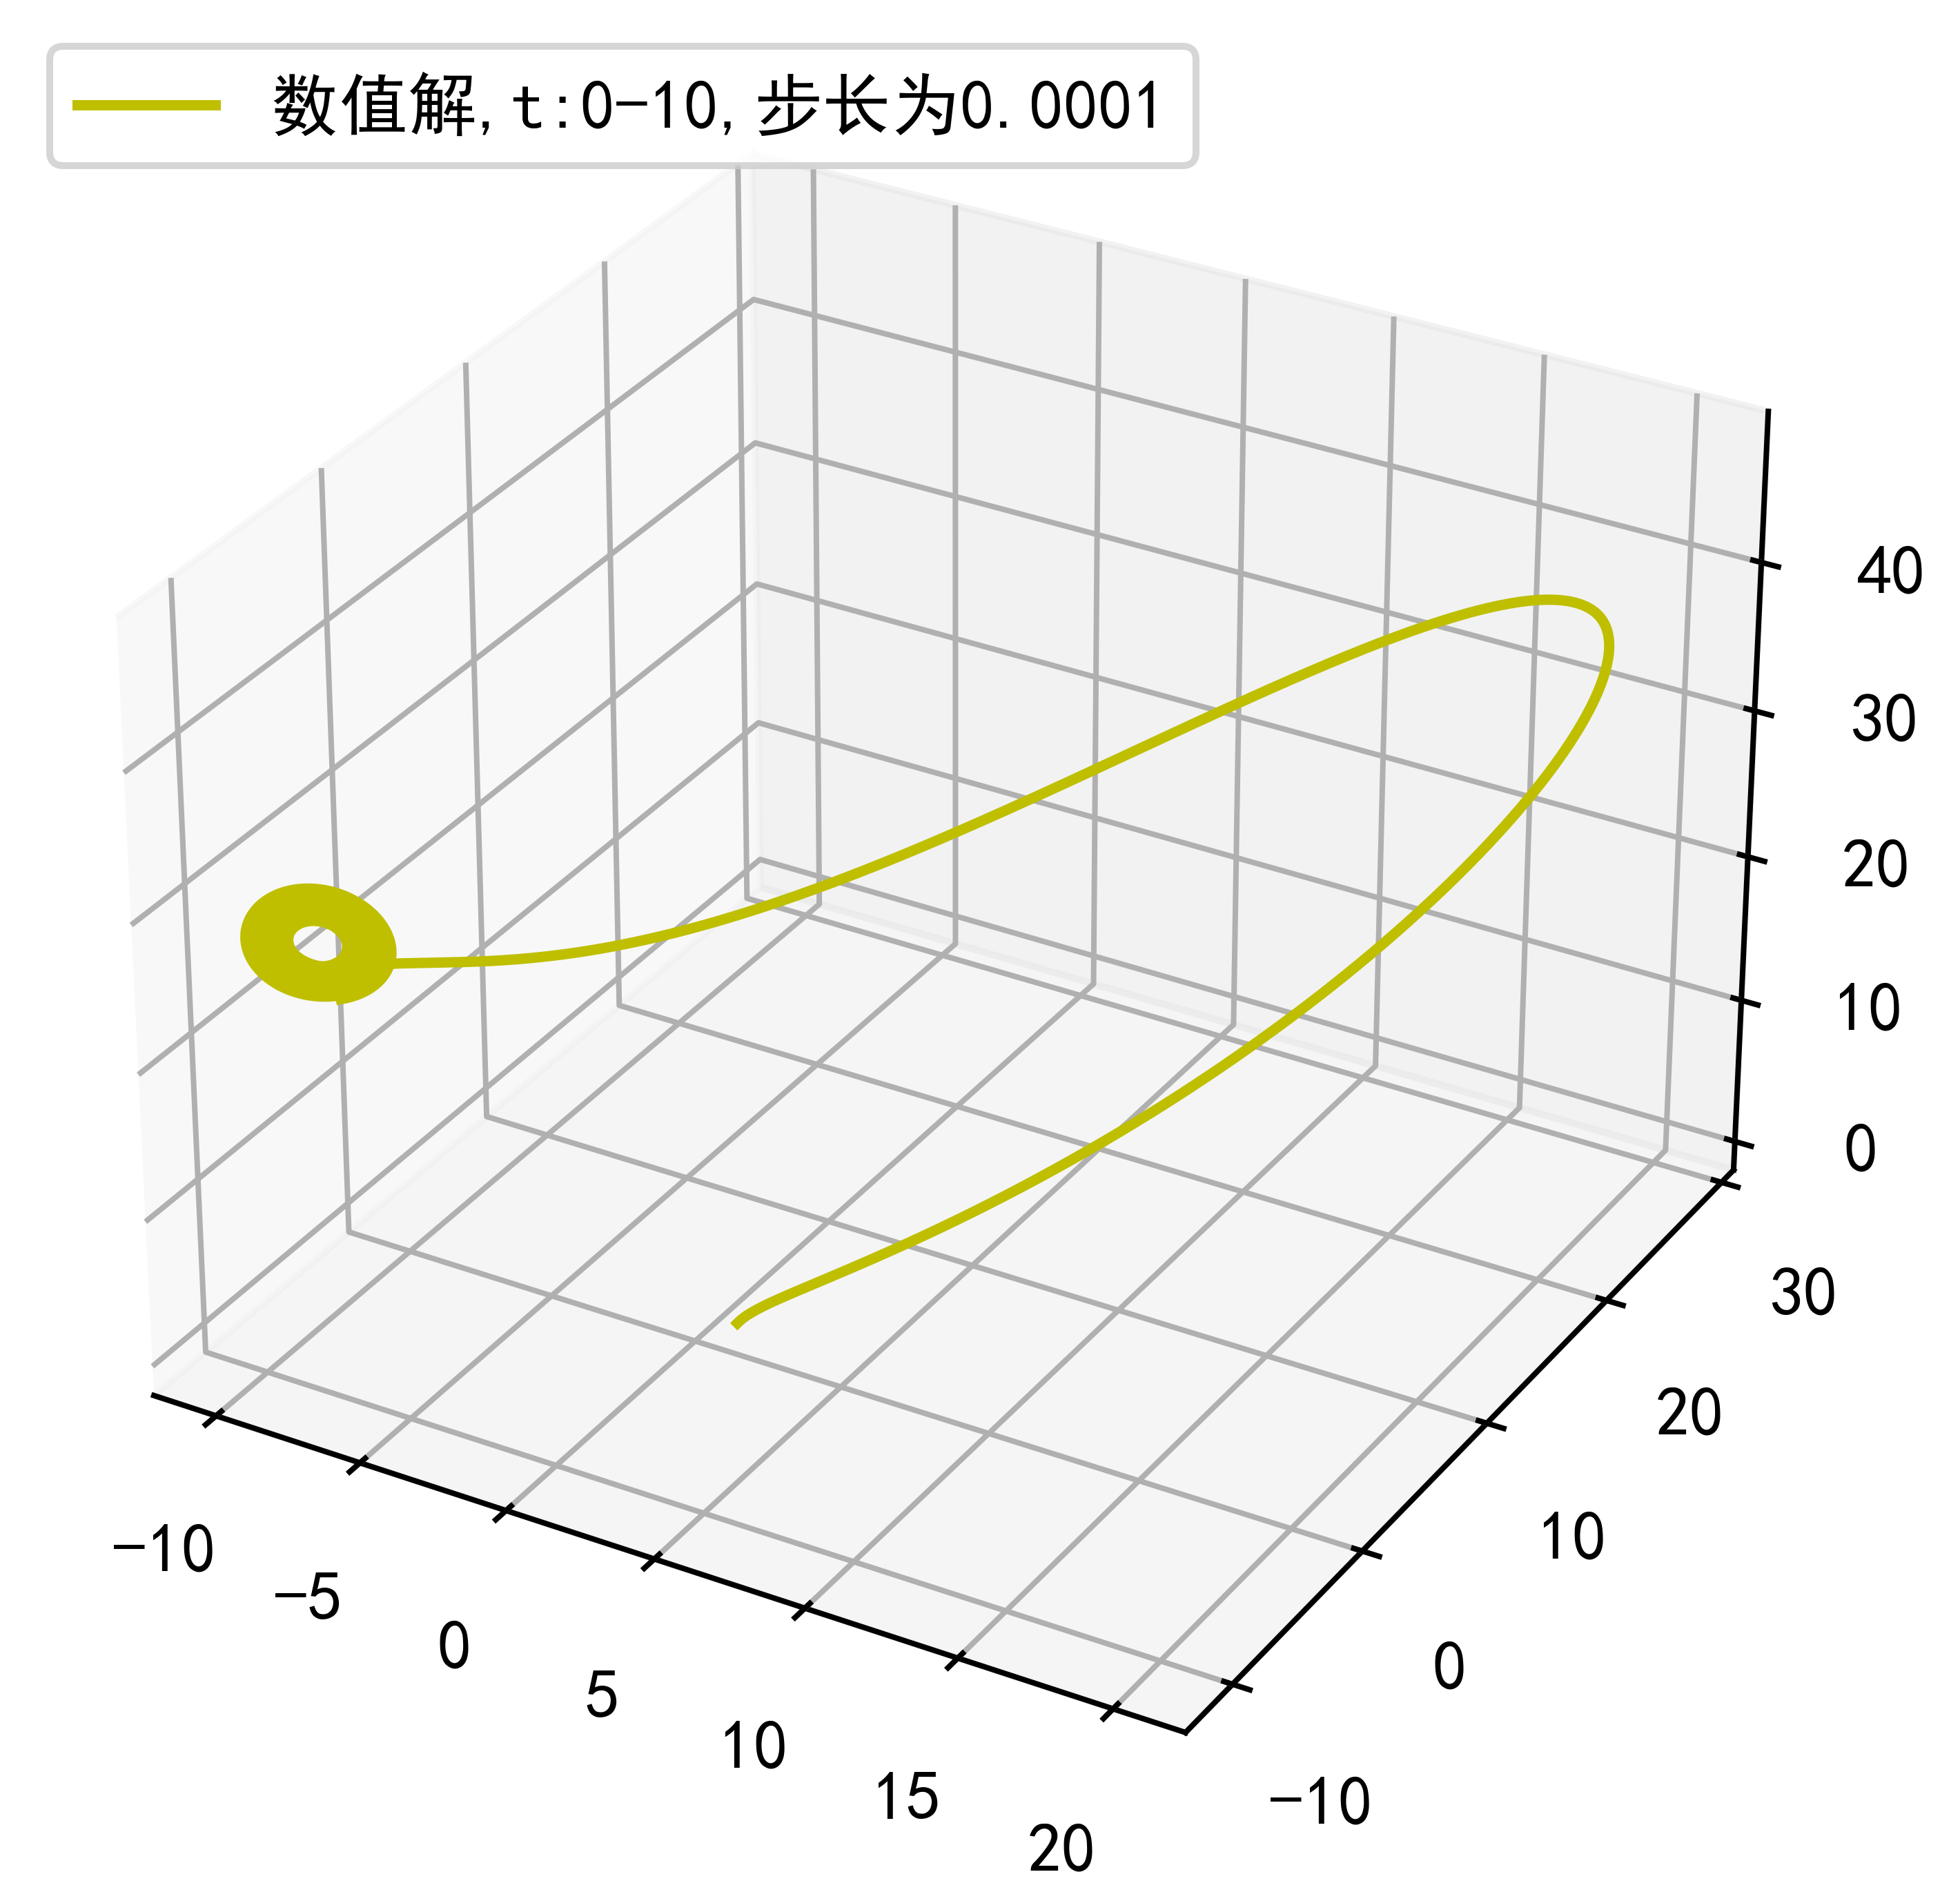
\includegraphics[scale=0.65]{21}
    \caption{起始点为(1,1,-1)}
    \end{minipage}
    \begin{minipage}{0.48\linewidth}
    \centering
    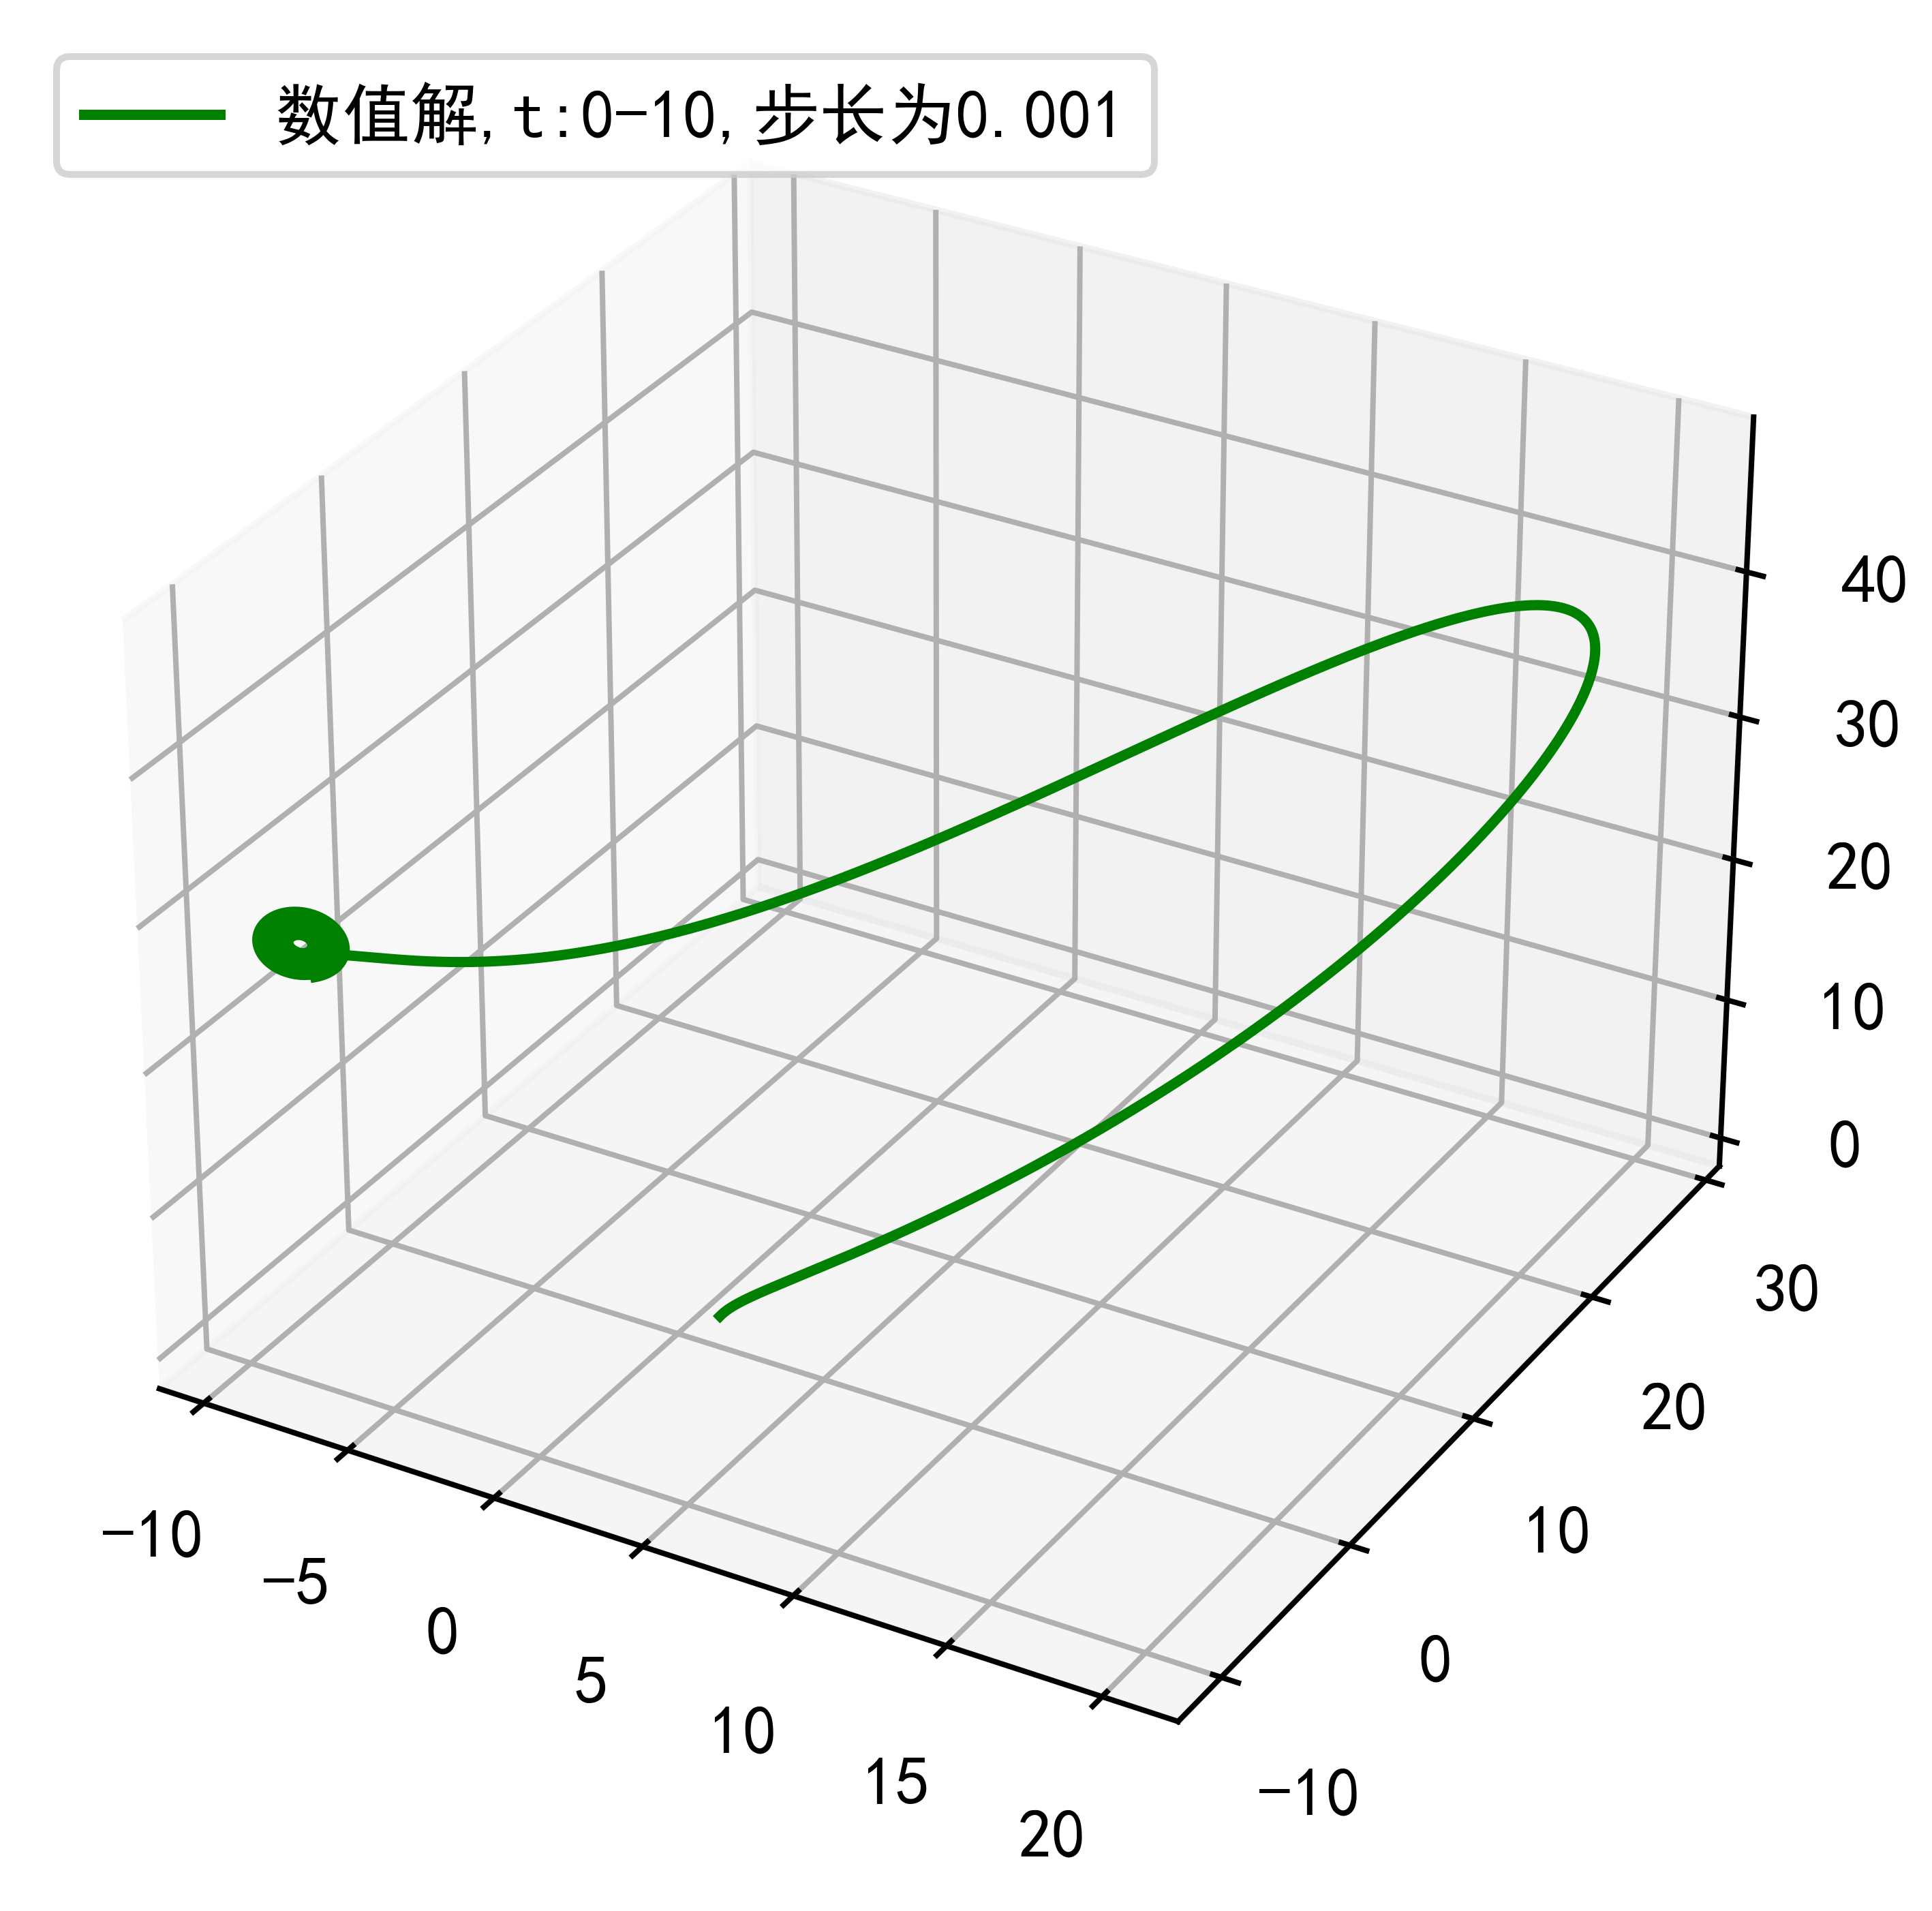
\includegraphics[scale=0.65]{22}
    \caption{起始点为(1,1,-1)}
    \end{minipage}
\end{figure}
\begin{figure}[h]
    \begin{minipage}[h]{0.48\linewidth}
    \centering
    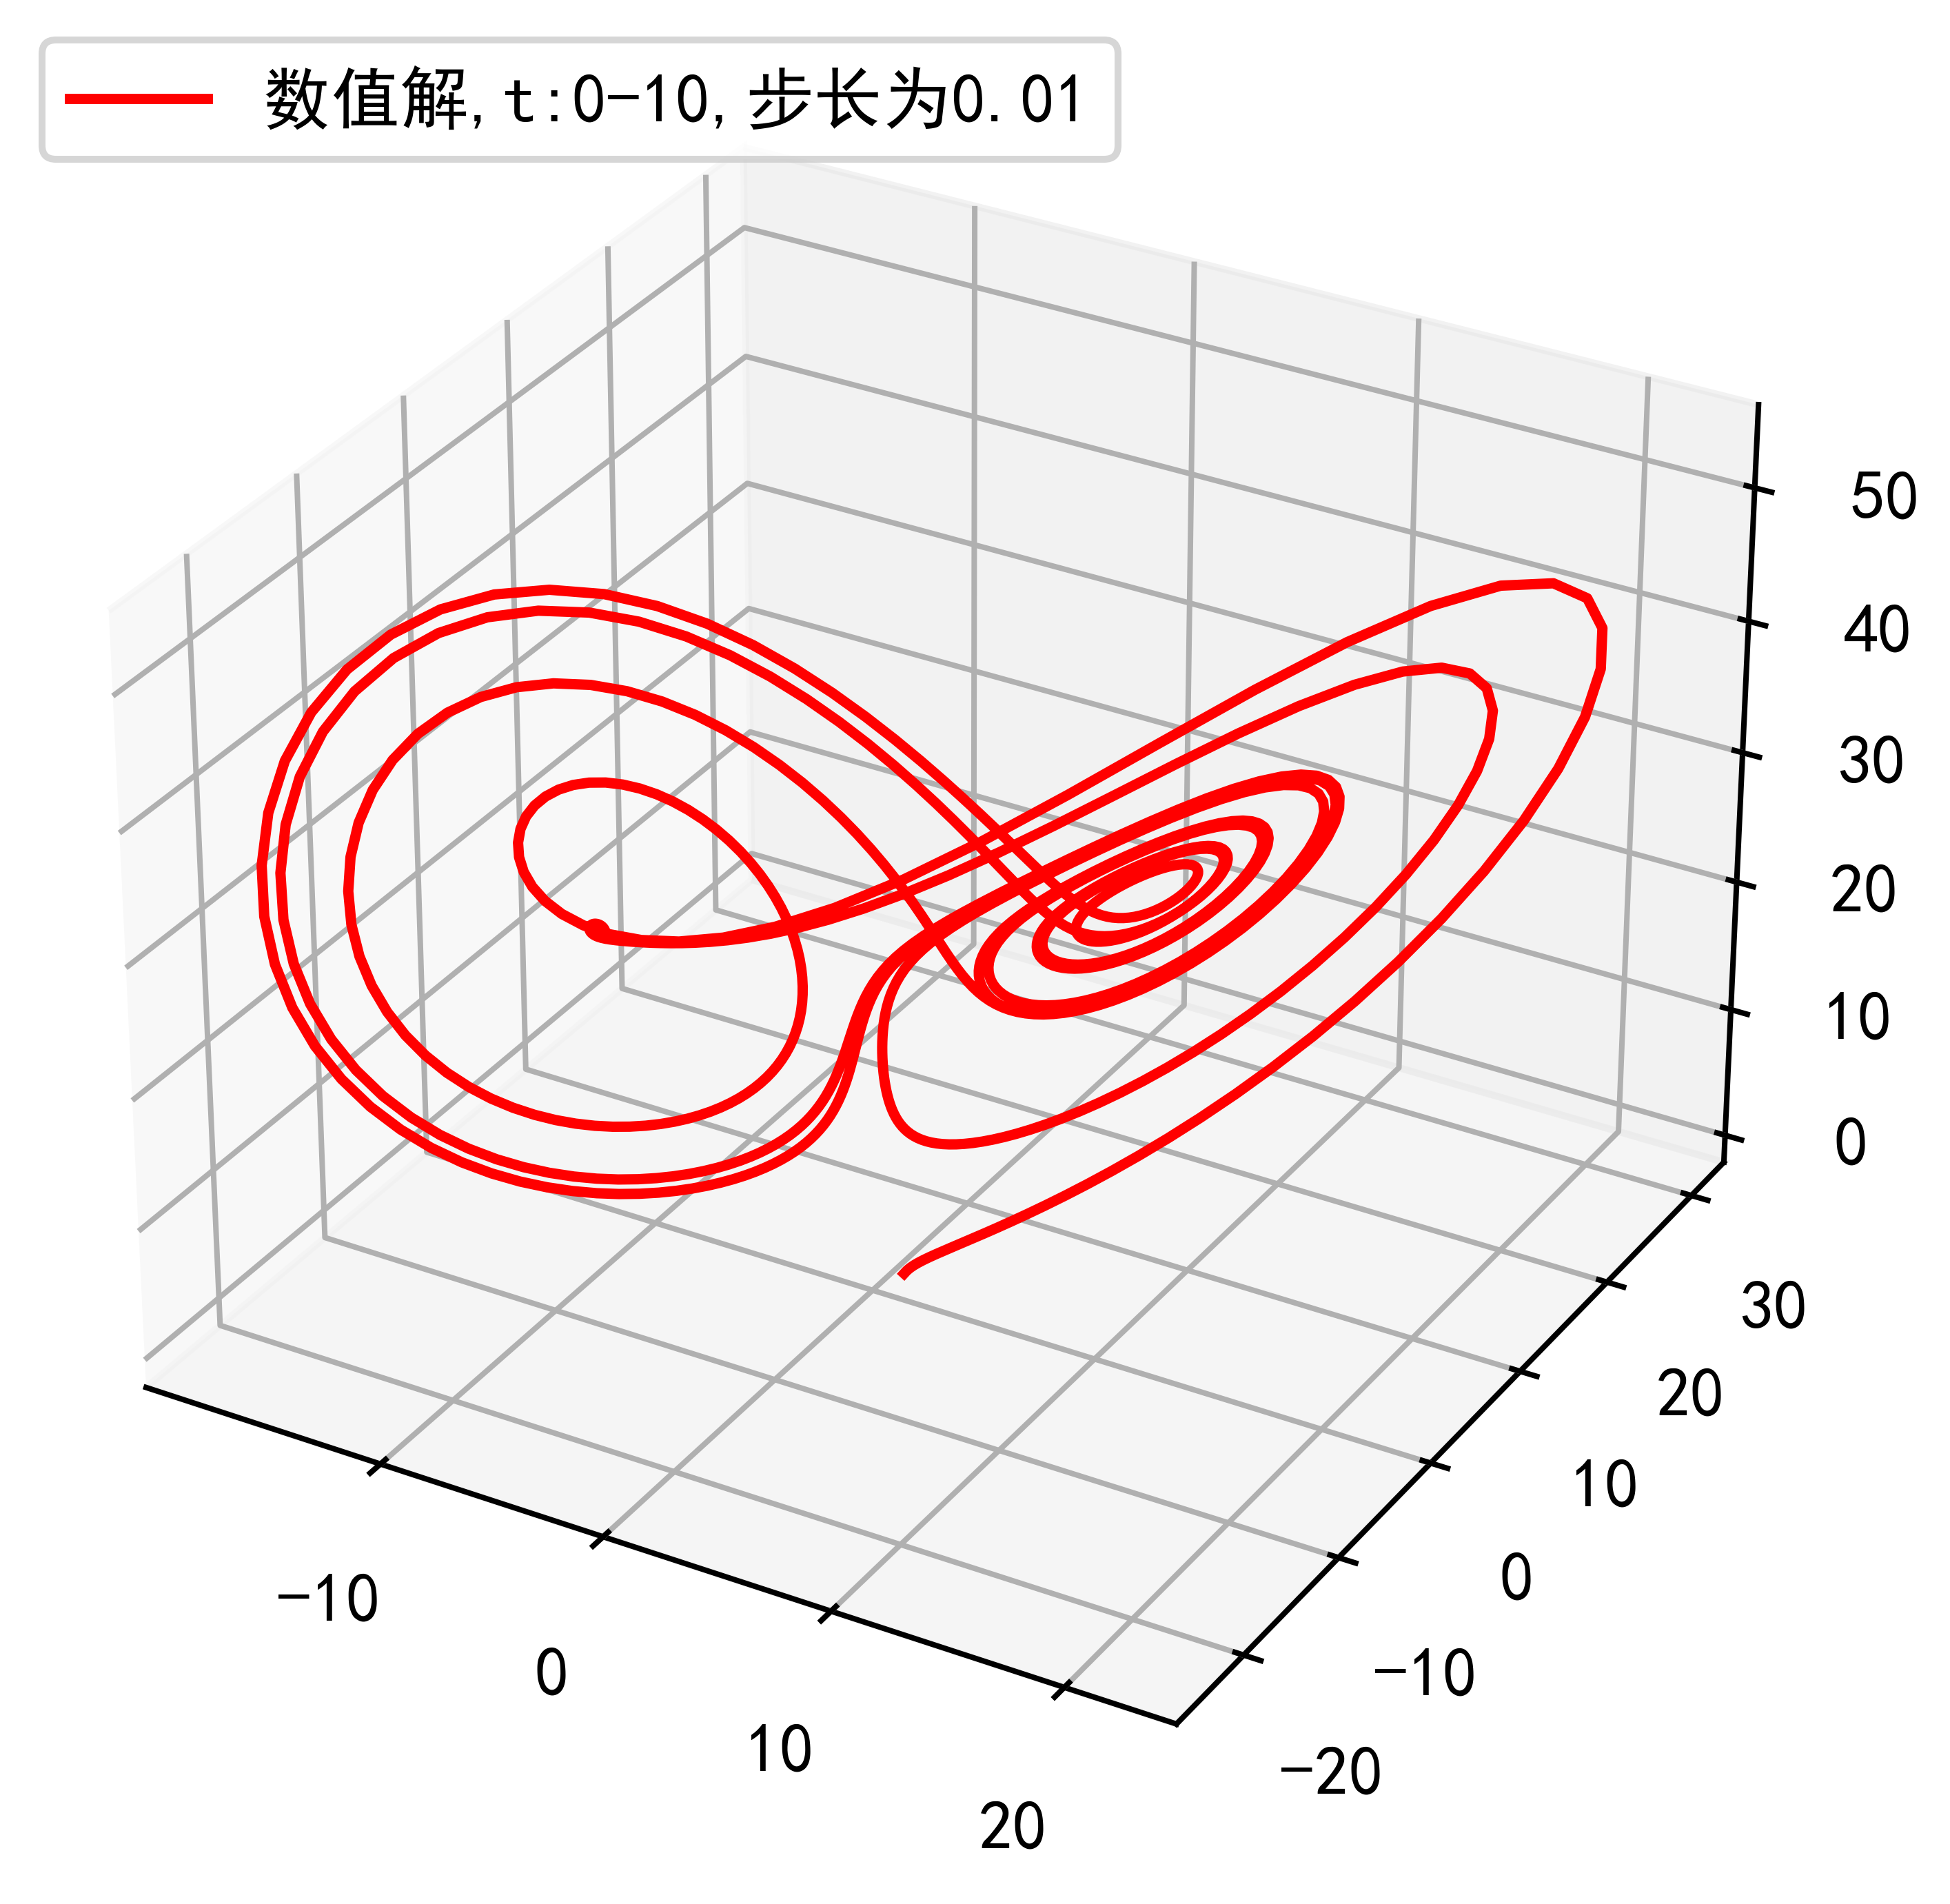
\includegraphics[scale=0.65]{23}
    \caption{起始点为(1,1,-1)}
    \end{minipage}
    \begin{minipage}[h]{0.48\linewidth}
    \centering
    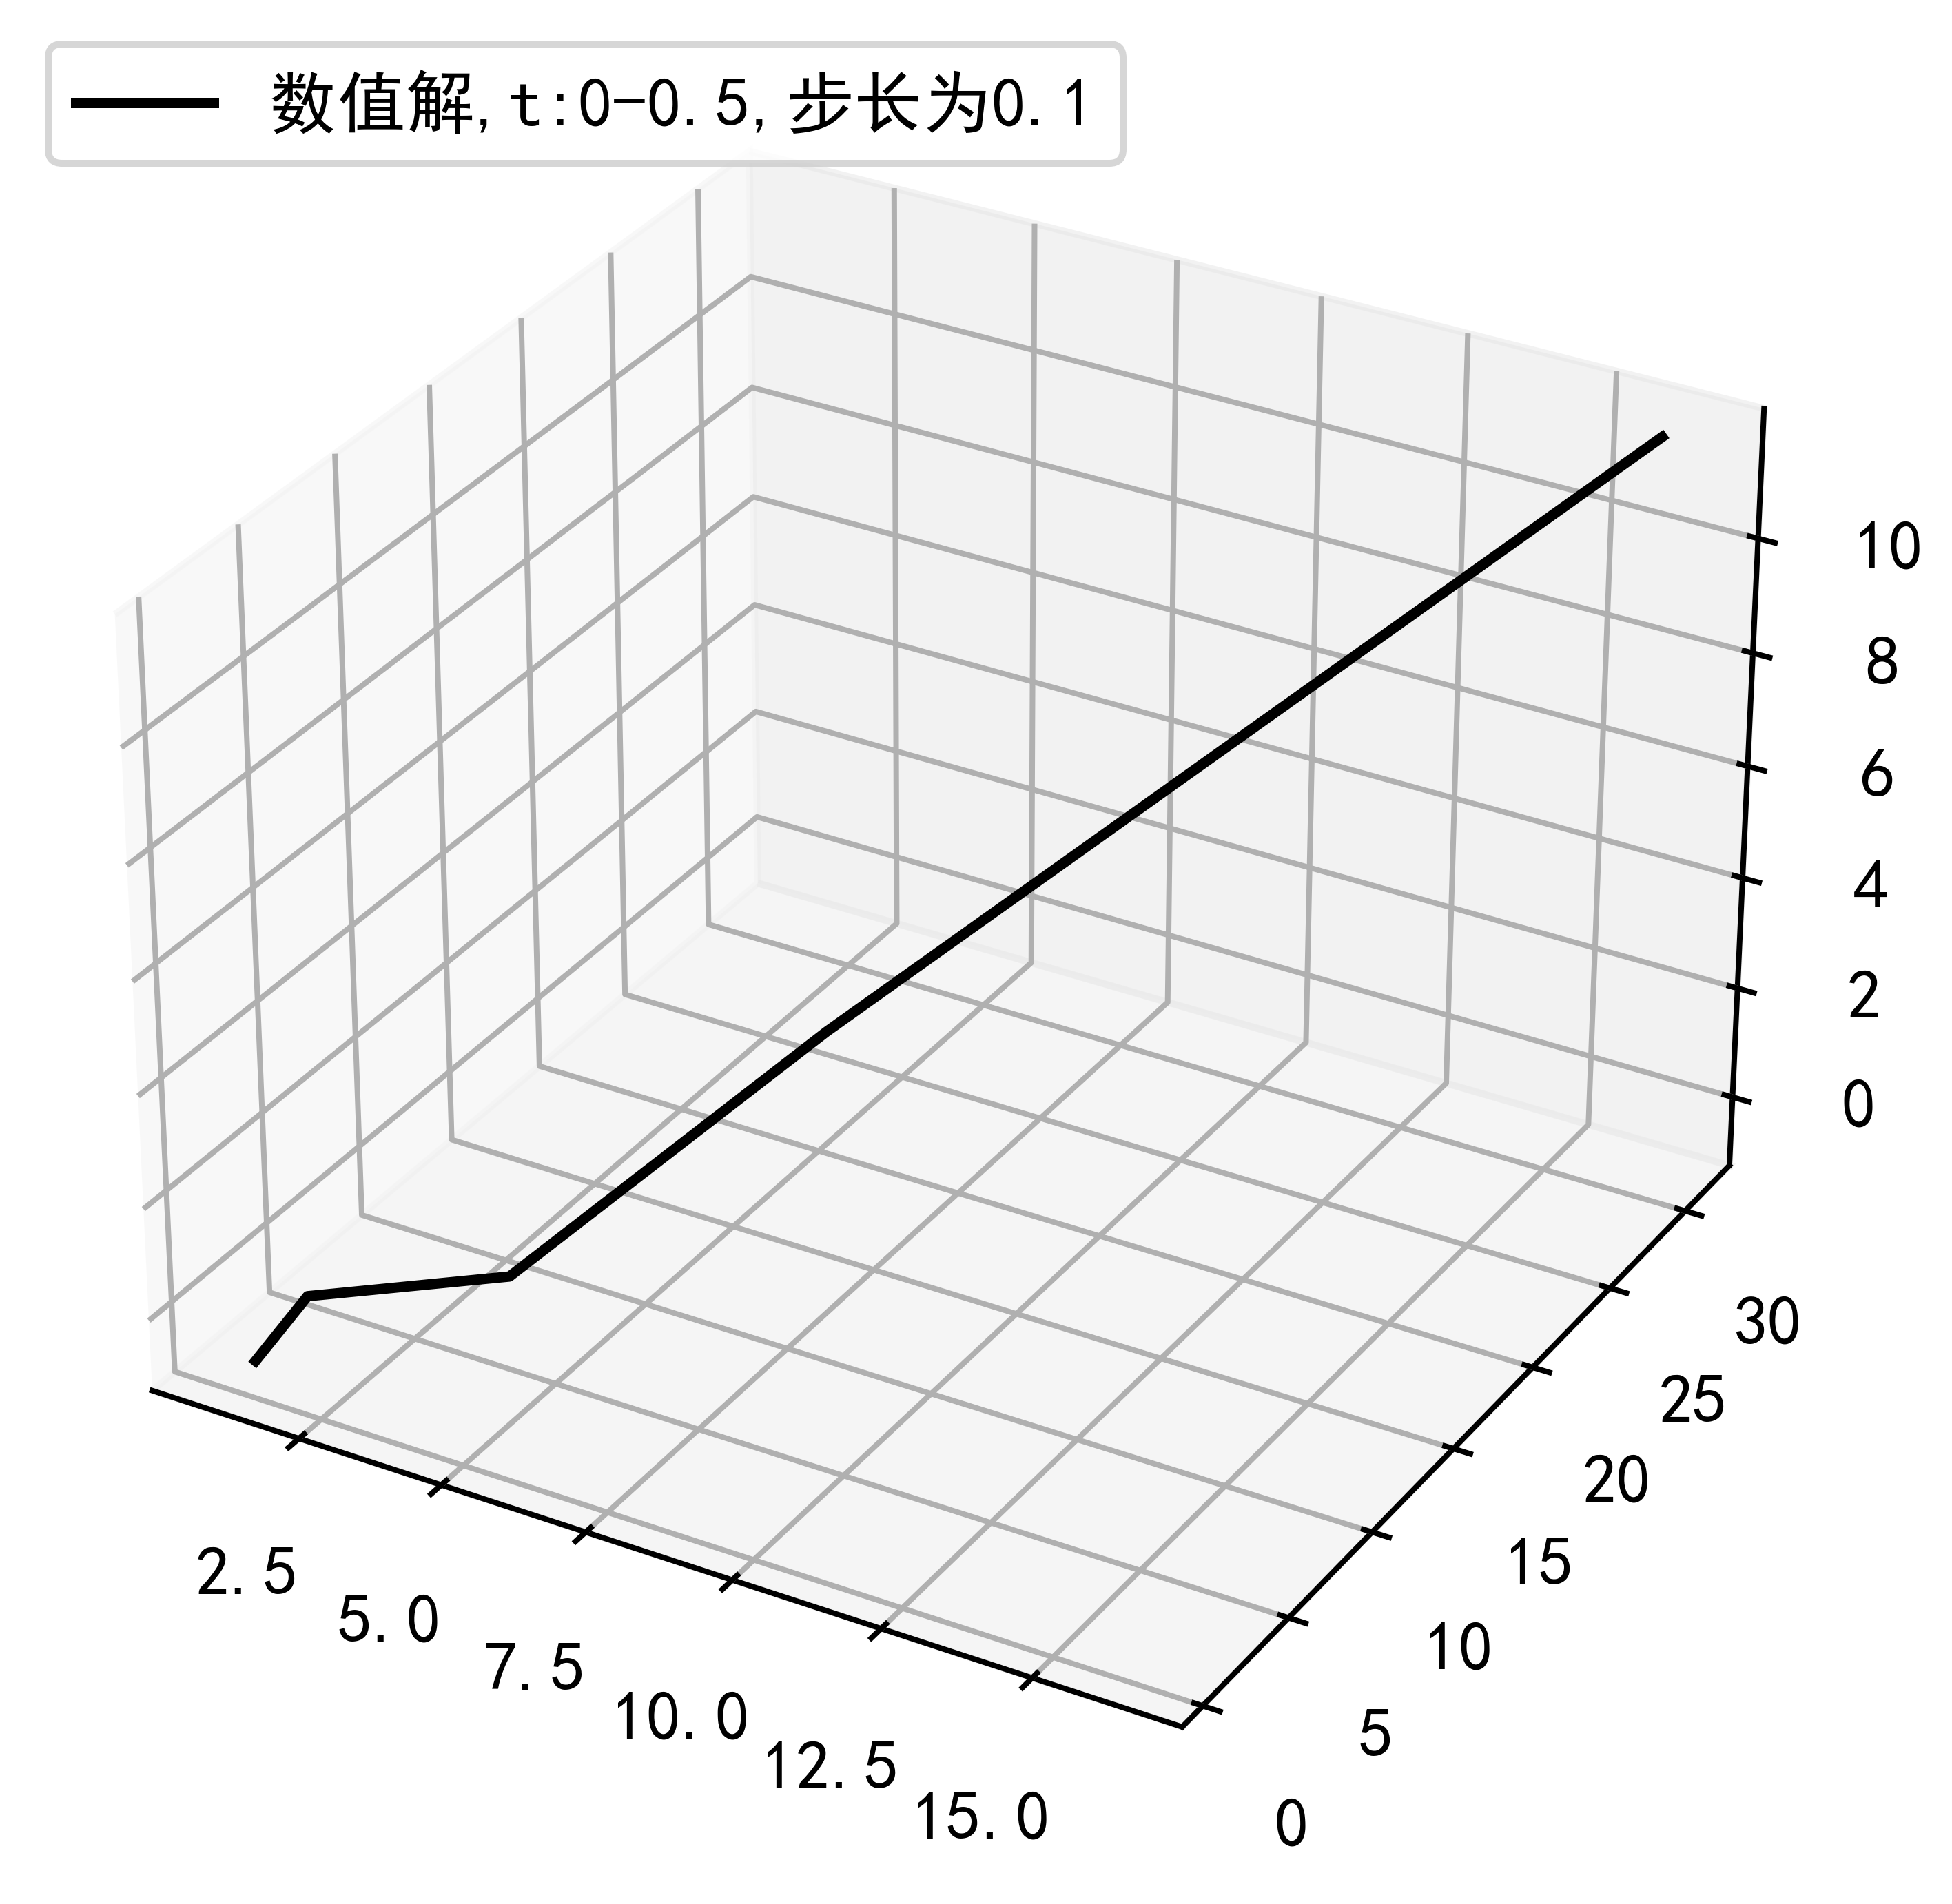
\includegraphics[scale=0.65]{24}
    \caption{起始点为(1,1,-1)}
    \end{minipage}
\end{figure}
\begin{figure}[H]
    \centering
    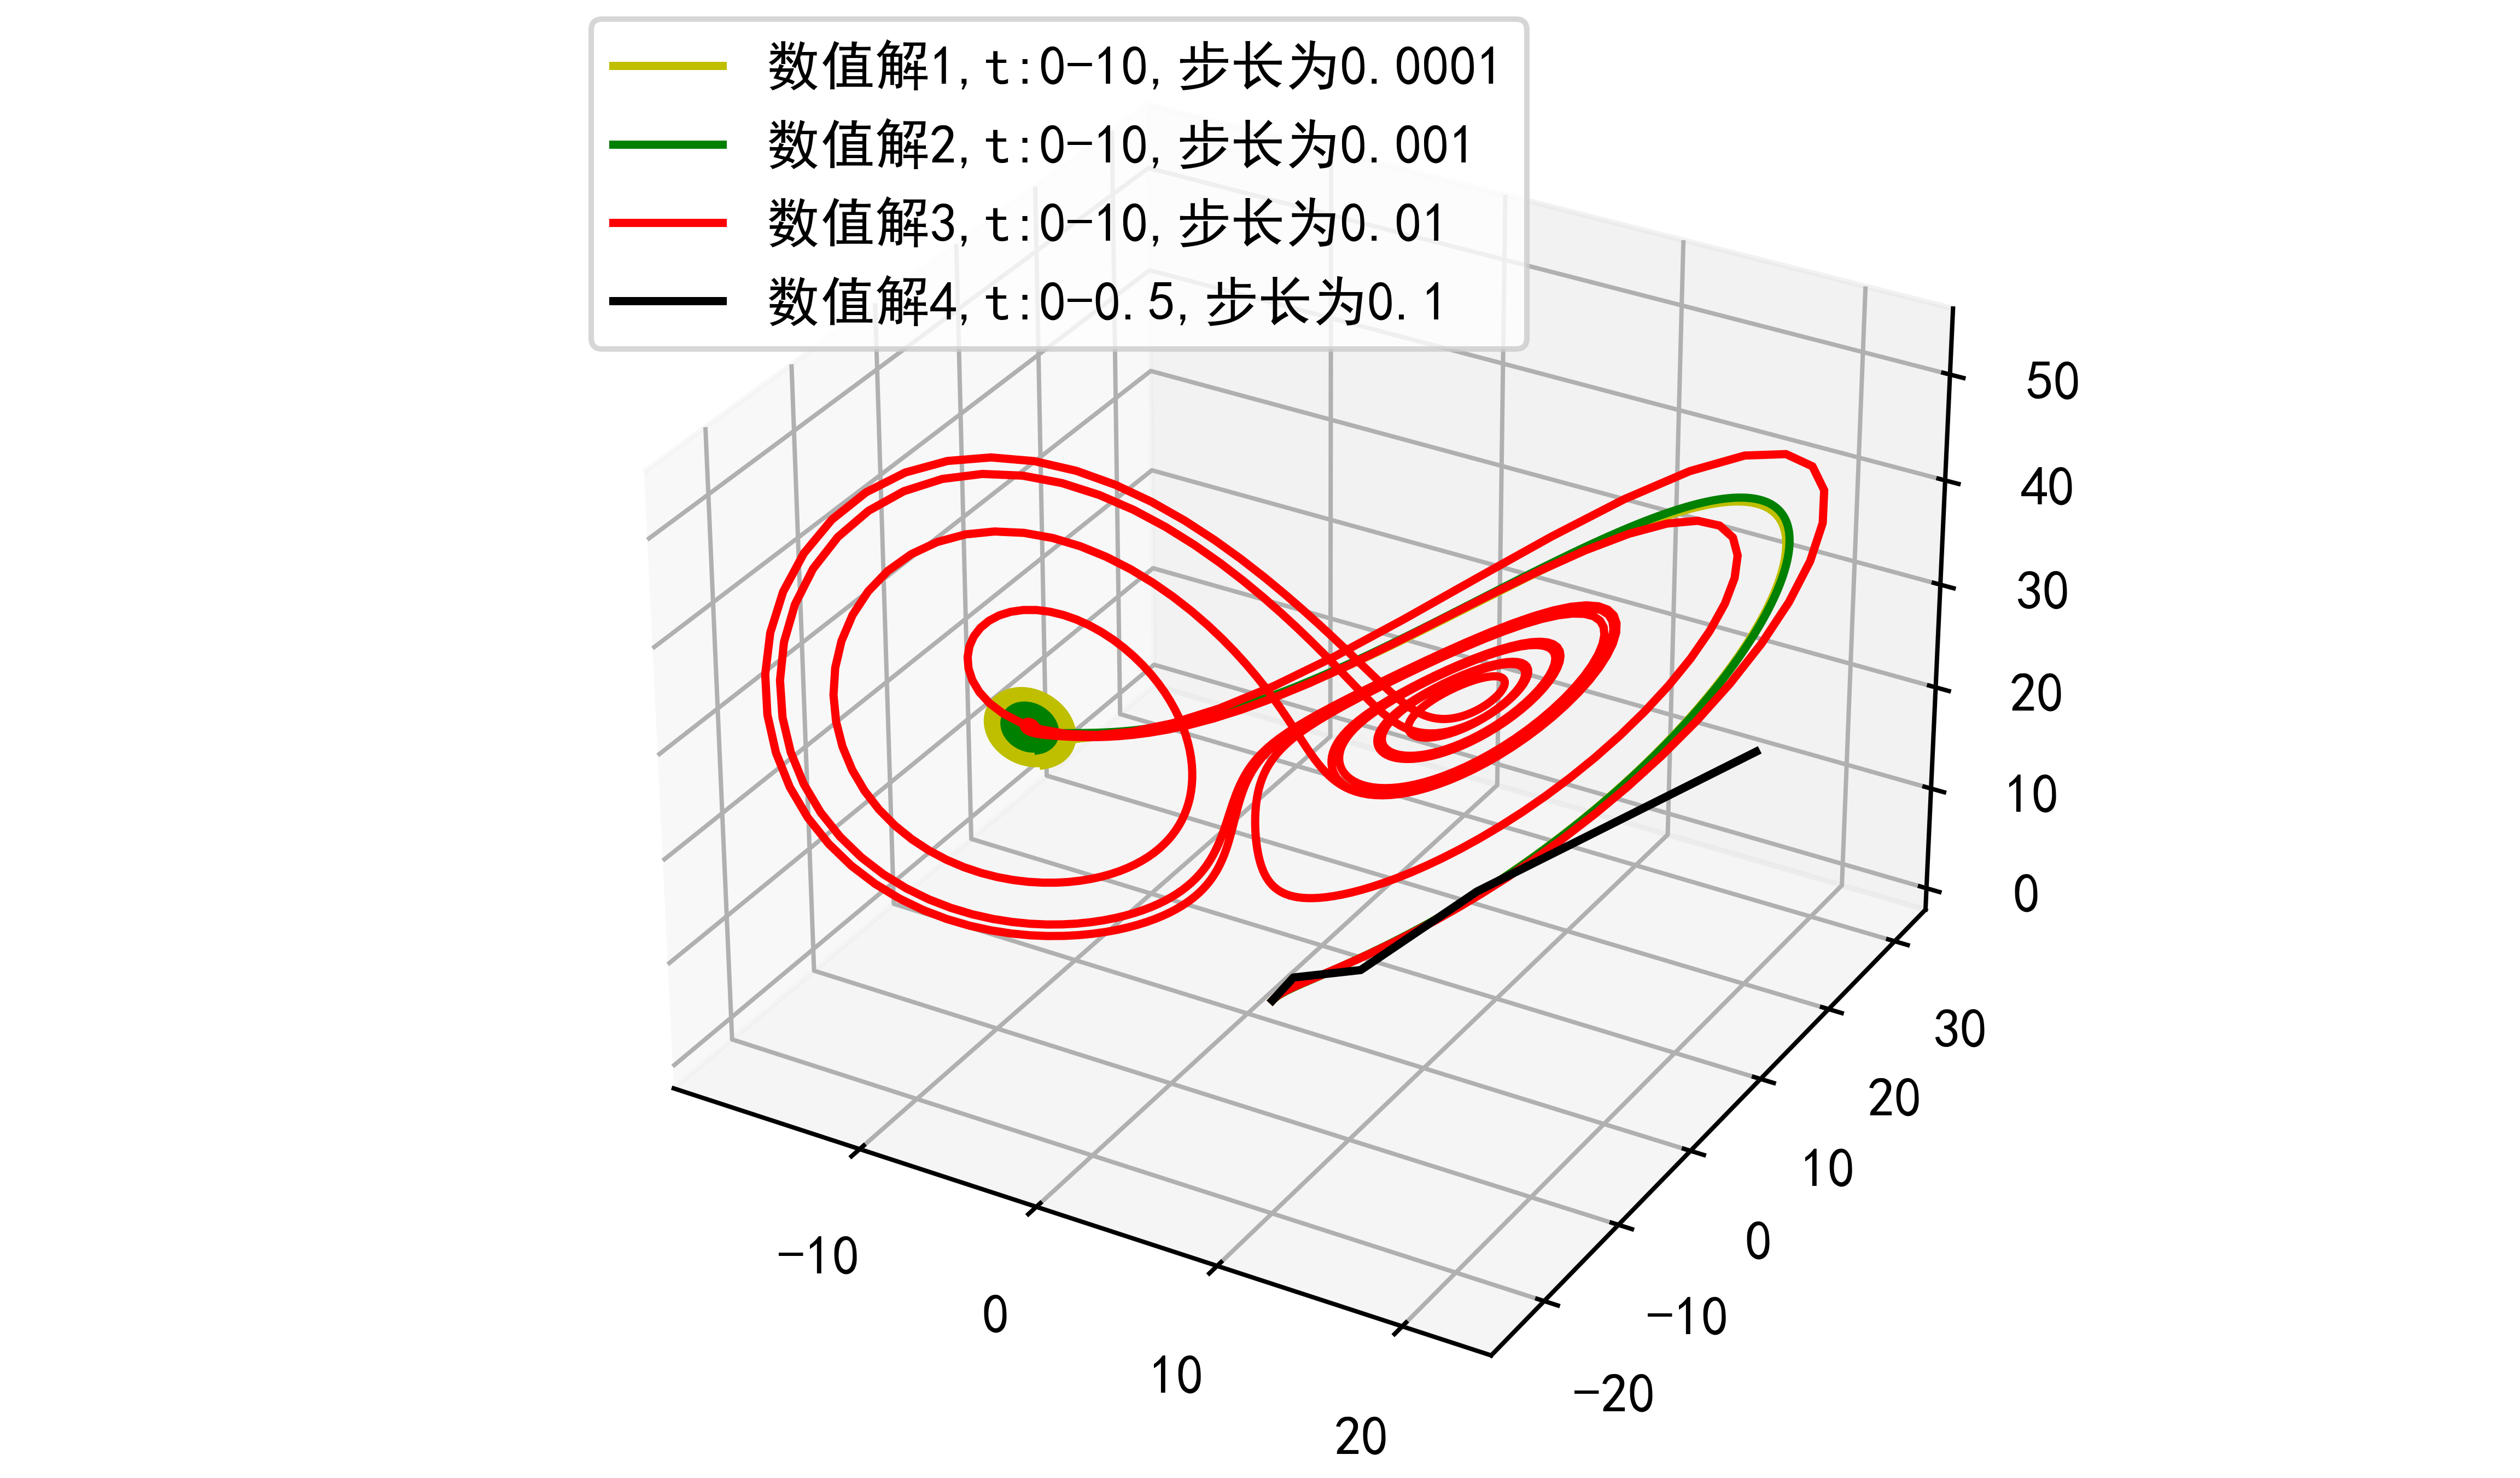
\includegraphics[scale=0.8]{25}
    \caption{起始点为(1,1,-1)}
\end{figure}

\begin{figure}[h]
    \begin{minipage}{0.48\linewidth}
    \centering
    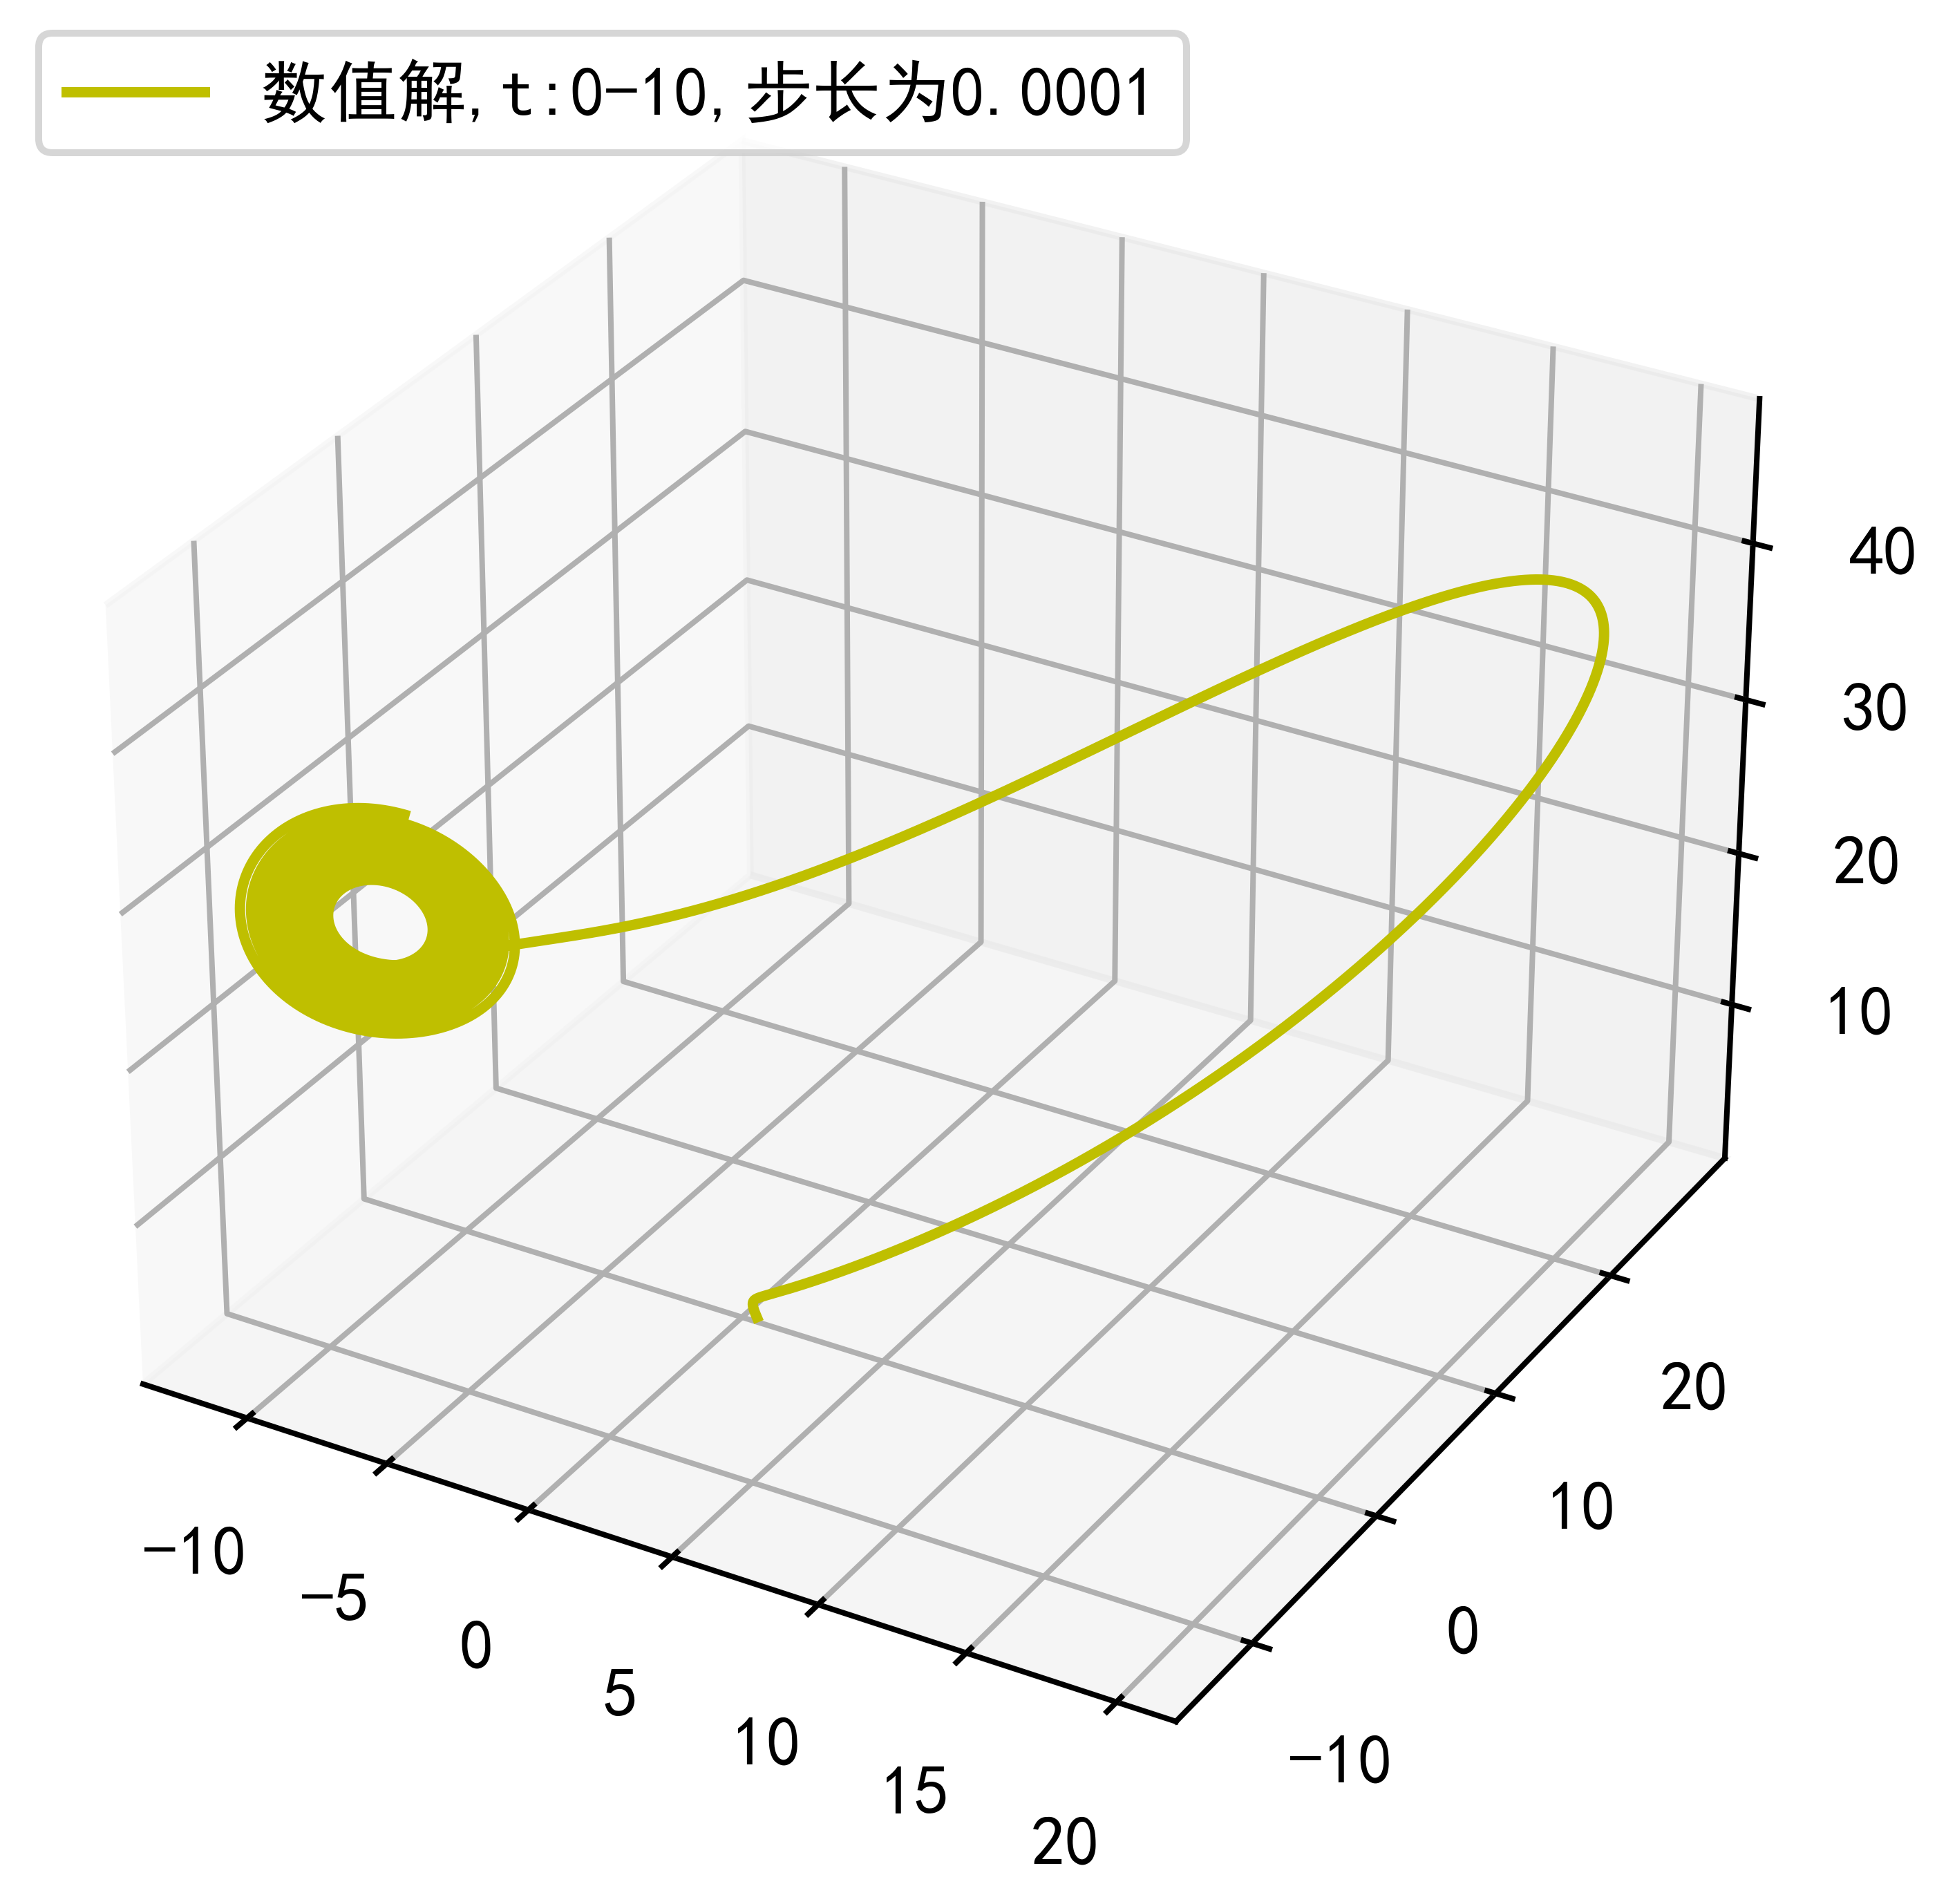
\includegraphics[scale=0.65]{31}
    \caption{起始点为(1,-1,1)}
    \end{minipage}
    \begin{minipage}{0.48\linewidth}
    \centering
    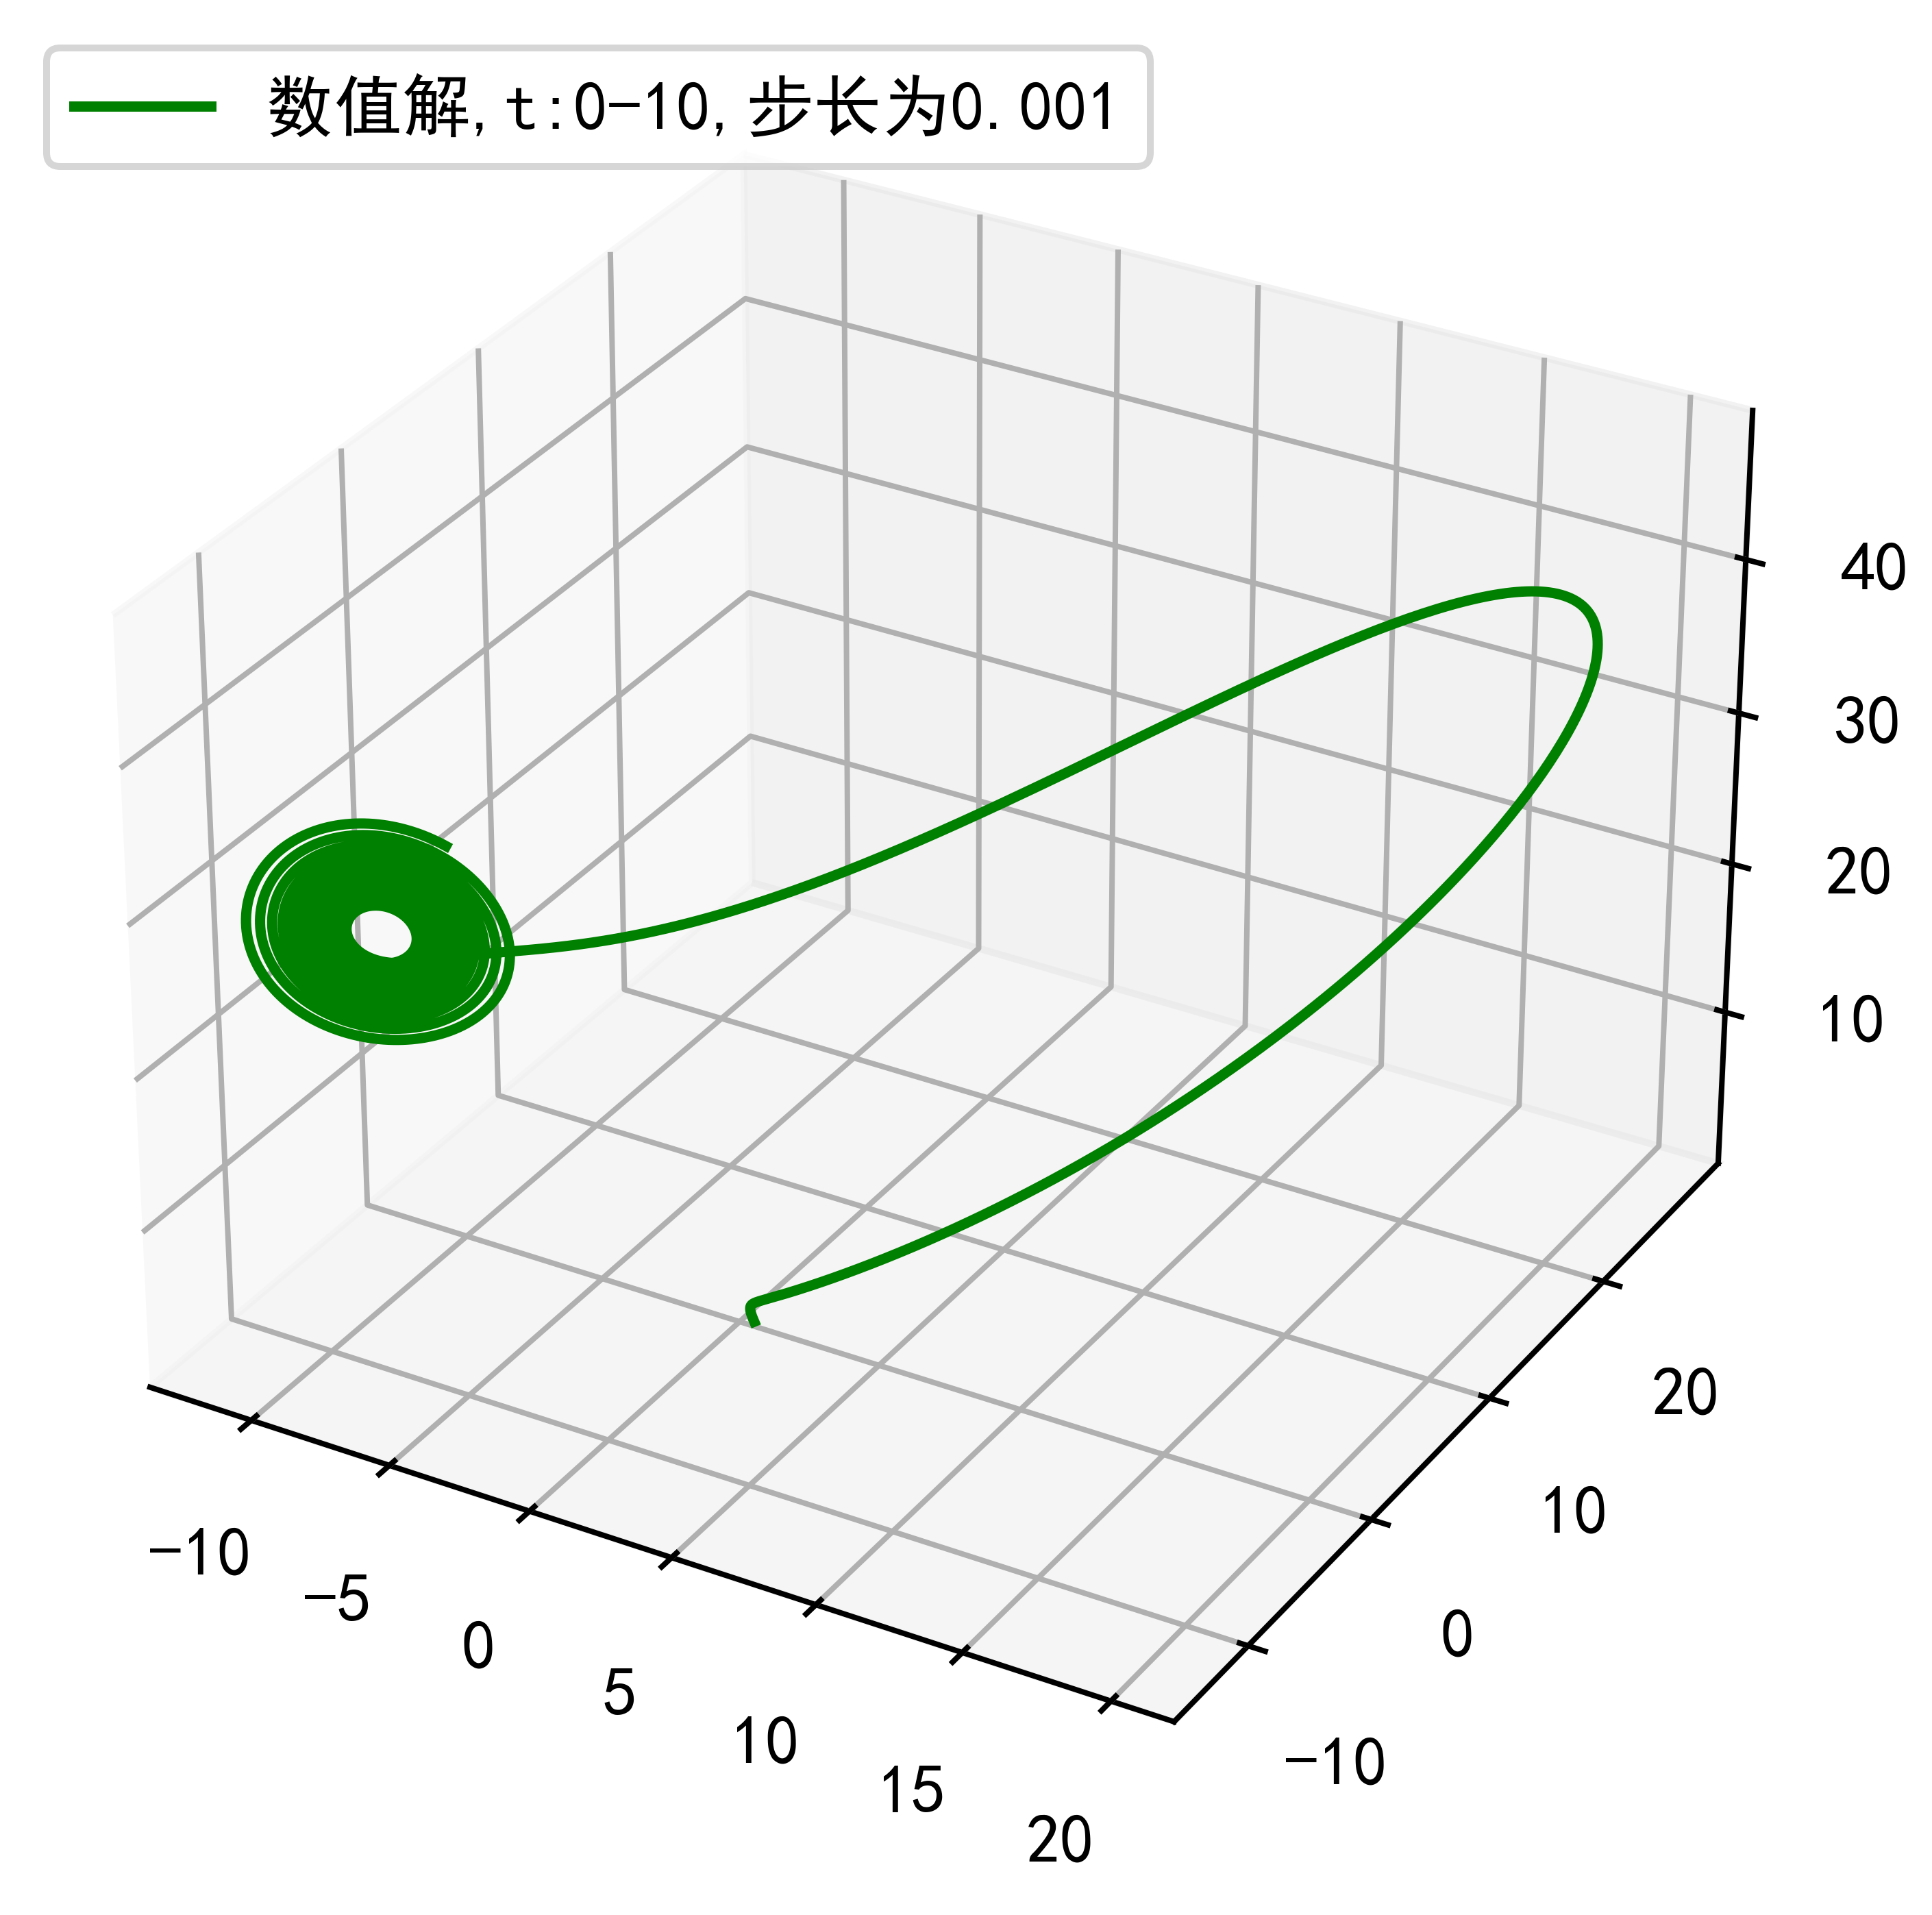
\includegraphics[scale=0.65]{32}
    \caption{起始点为(1,-1,1)}
    \end{minipage}
\end{figure}
\begin{figure}[h]
    \begin{minipage}[h]{0.48\linewidth}
    \centering
    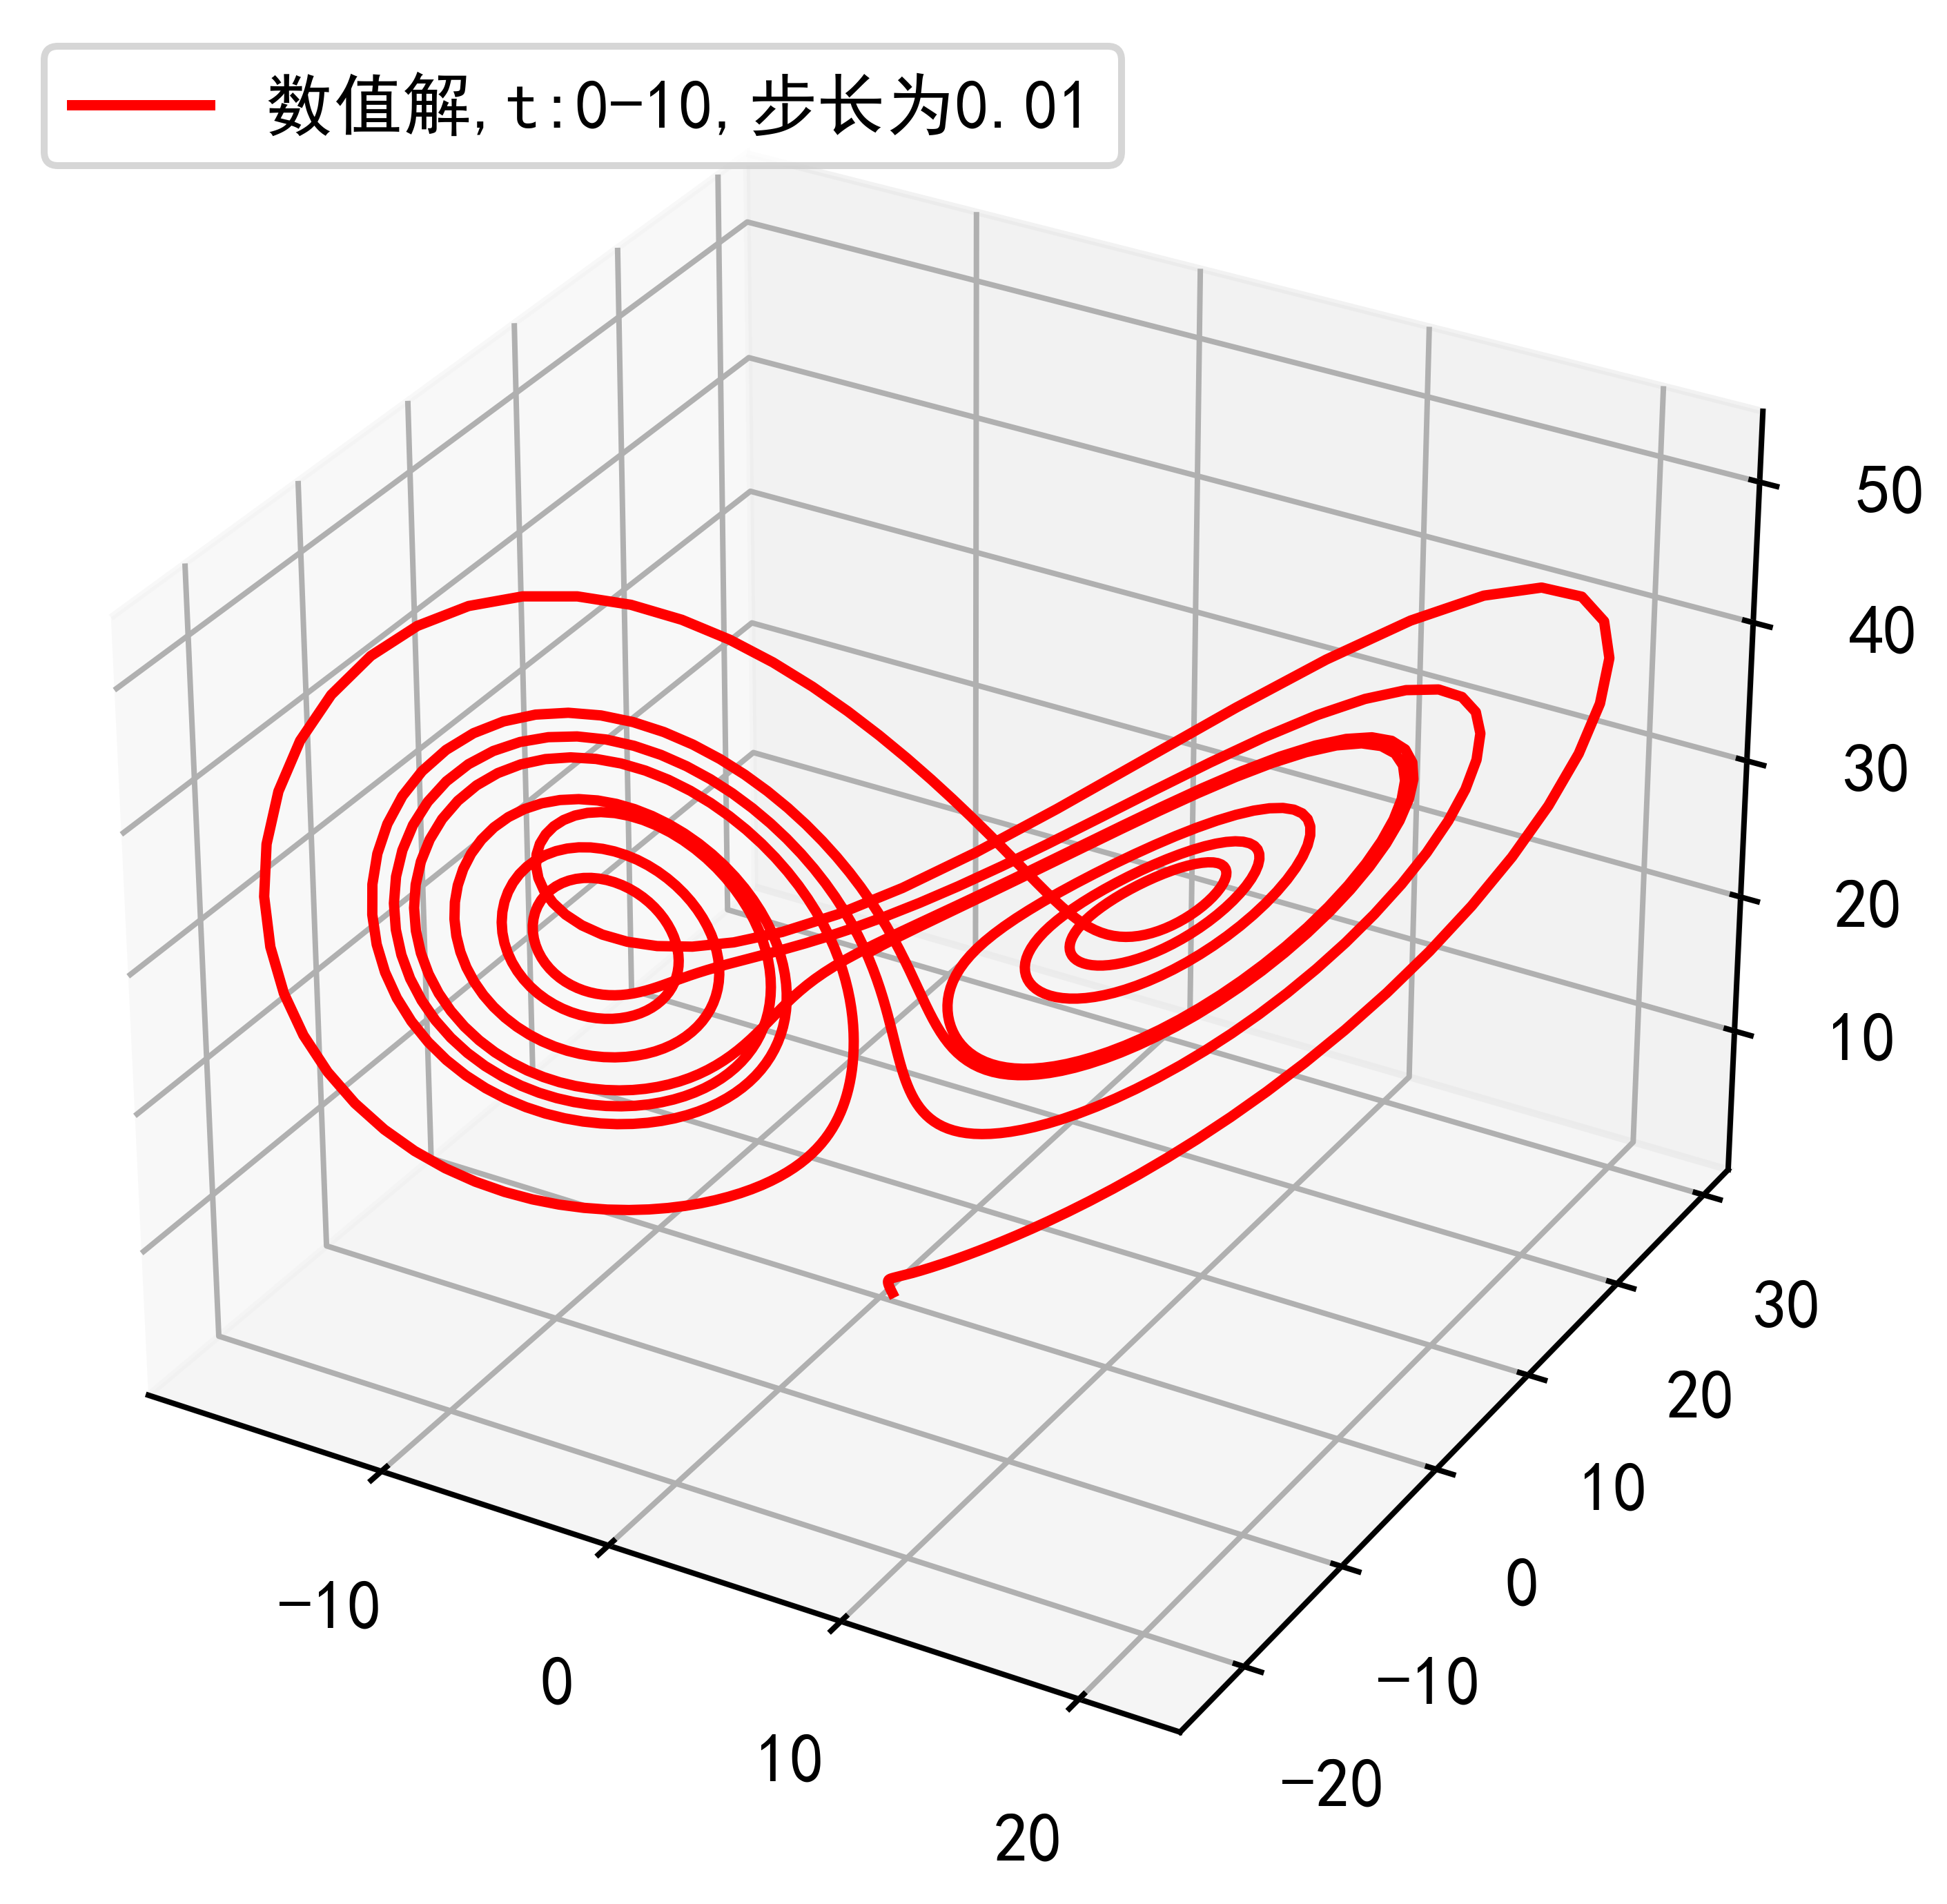
\includegraphics[scale=0.65]{33}
    \caption{起始点为(1,-1,1)}\end{minipage}
    \begin{minipage}[h]{0.48\linewidth}
    \centering
    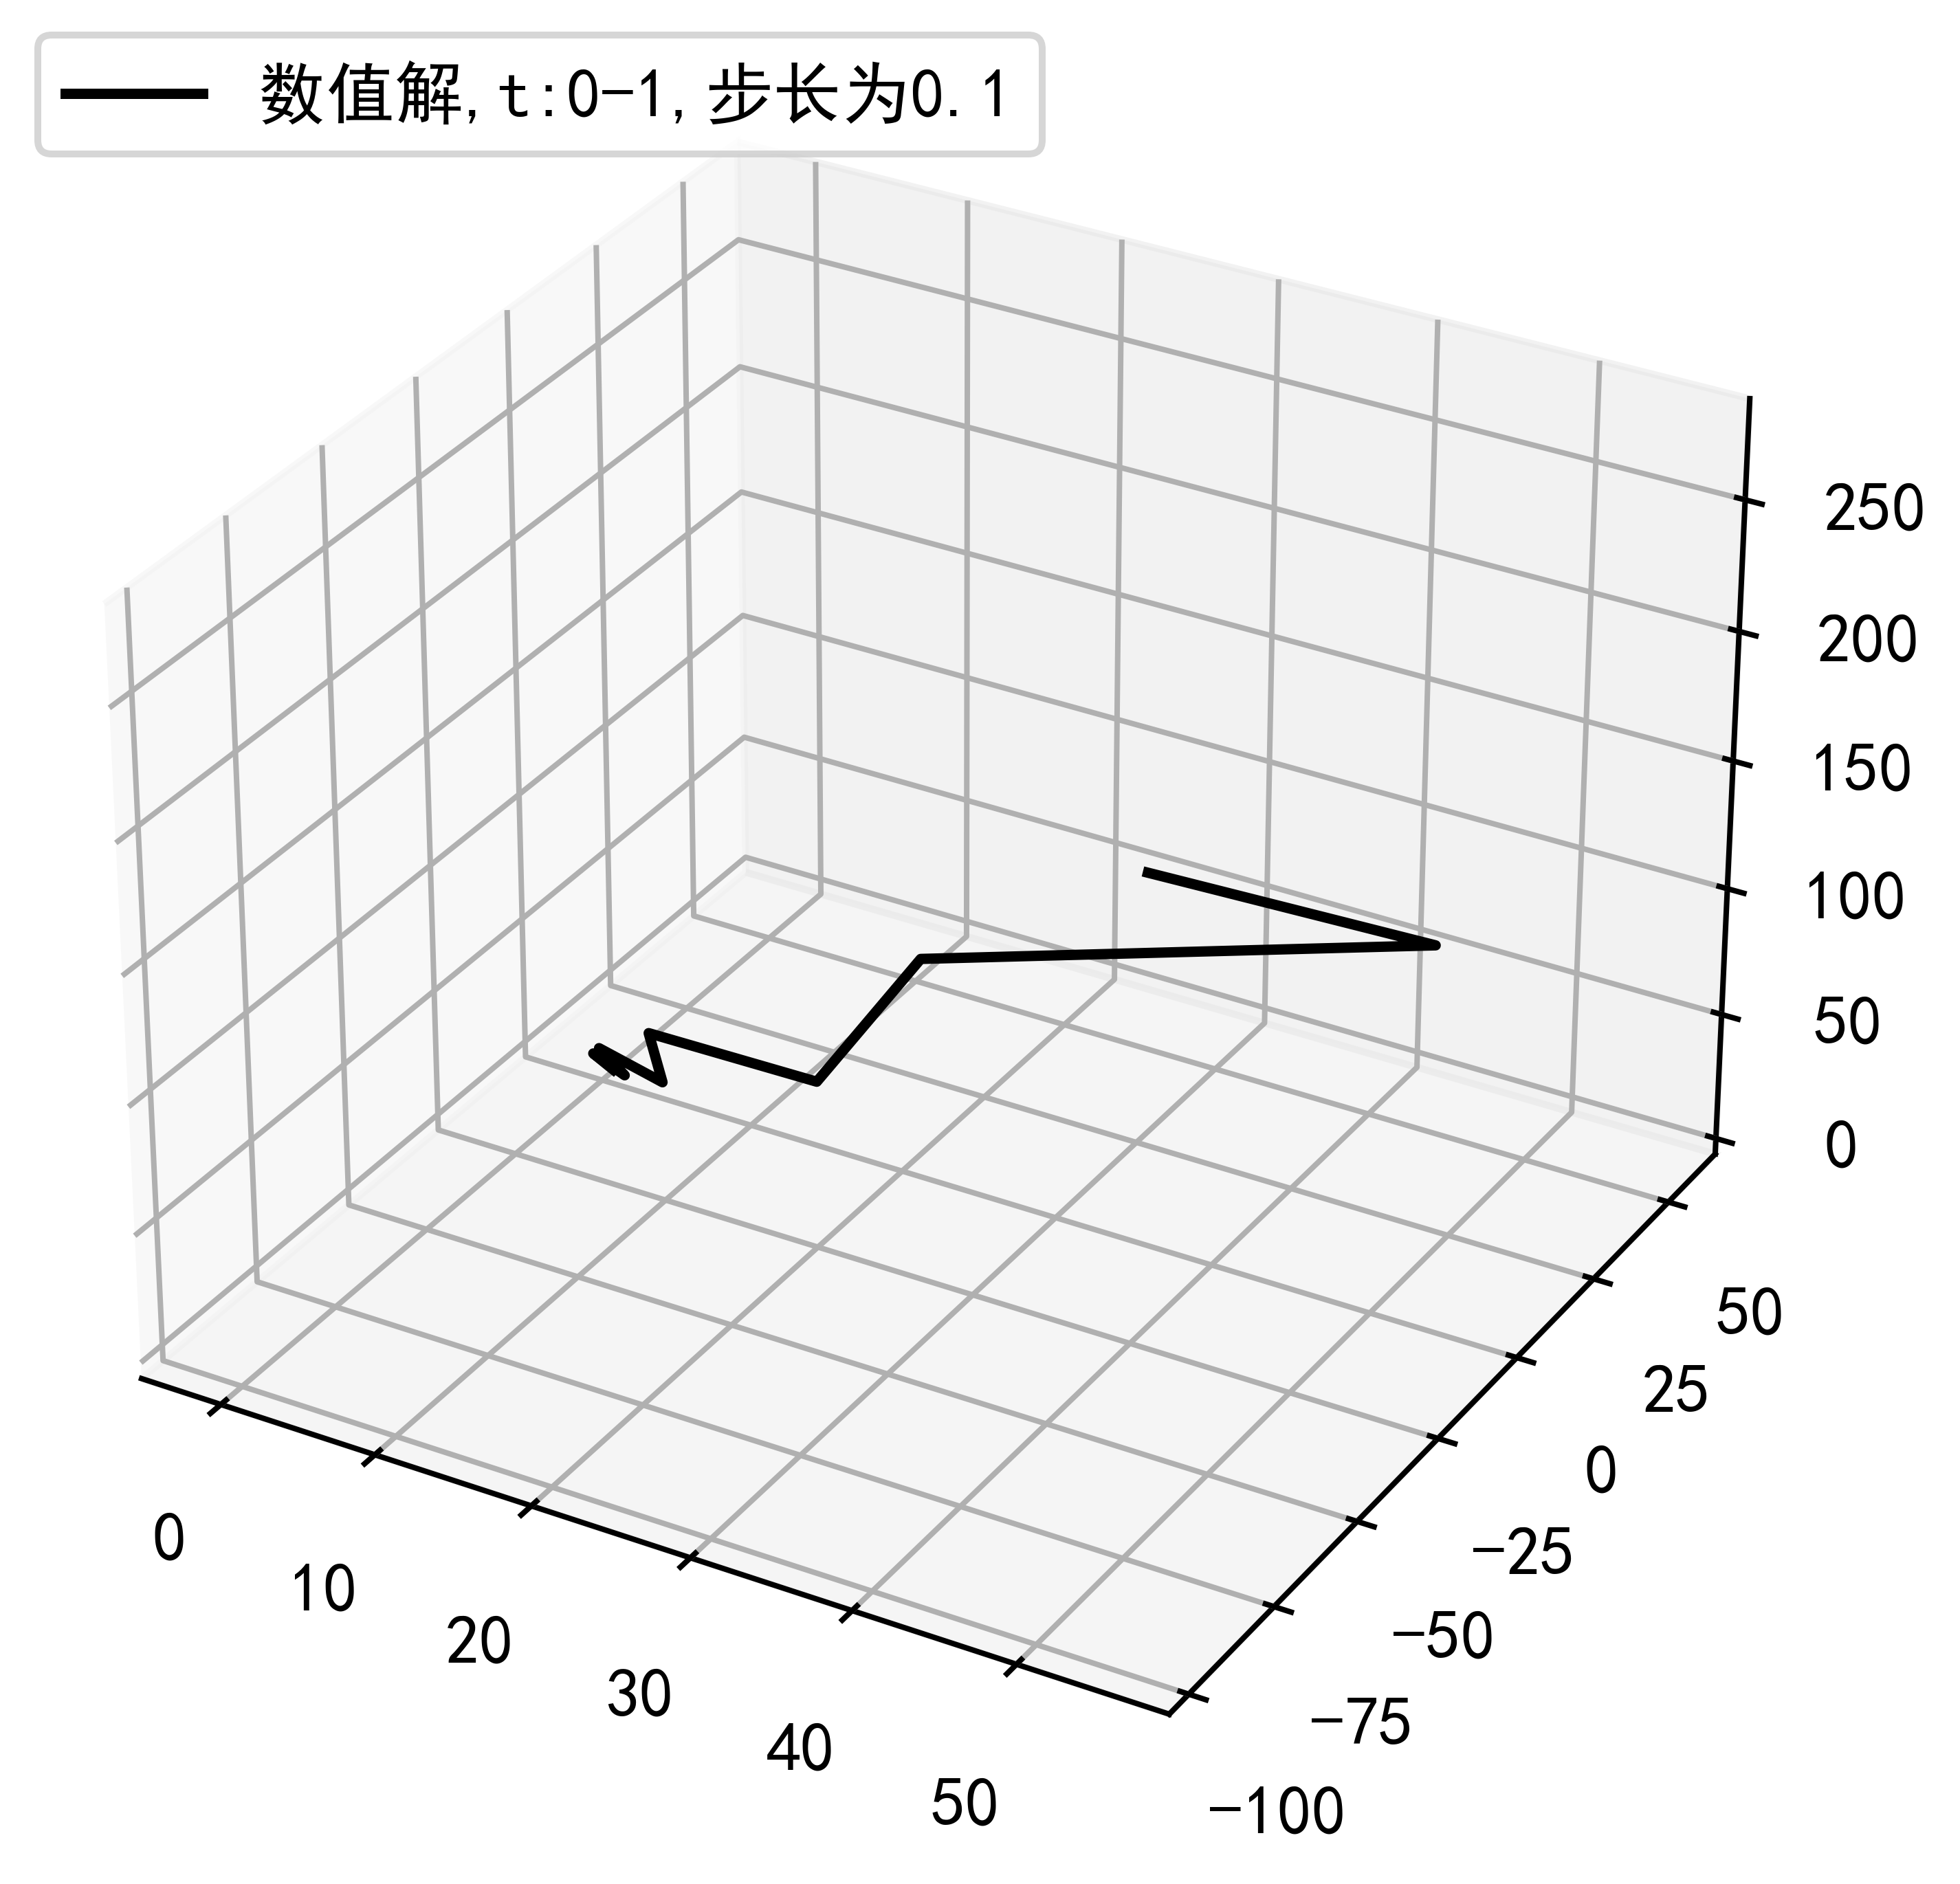
\includegraphics[scale=0.65]{34}
    \caption{起始点为(1,-1,1)}
    \end{minipage}
\end{figure}
\begin{figure}[H]
    \centering
    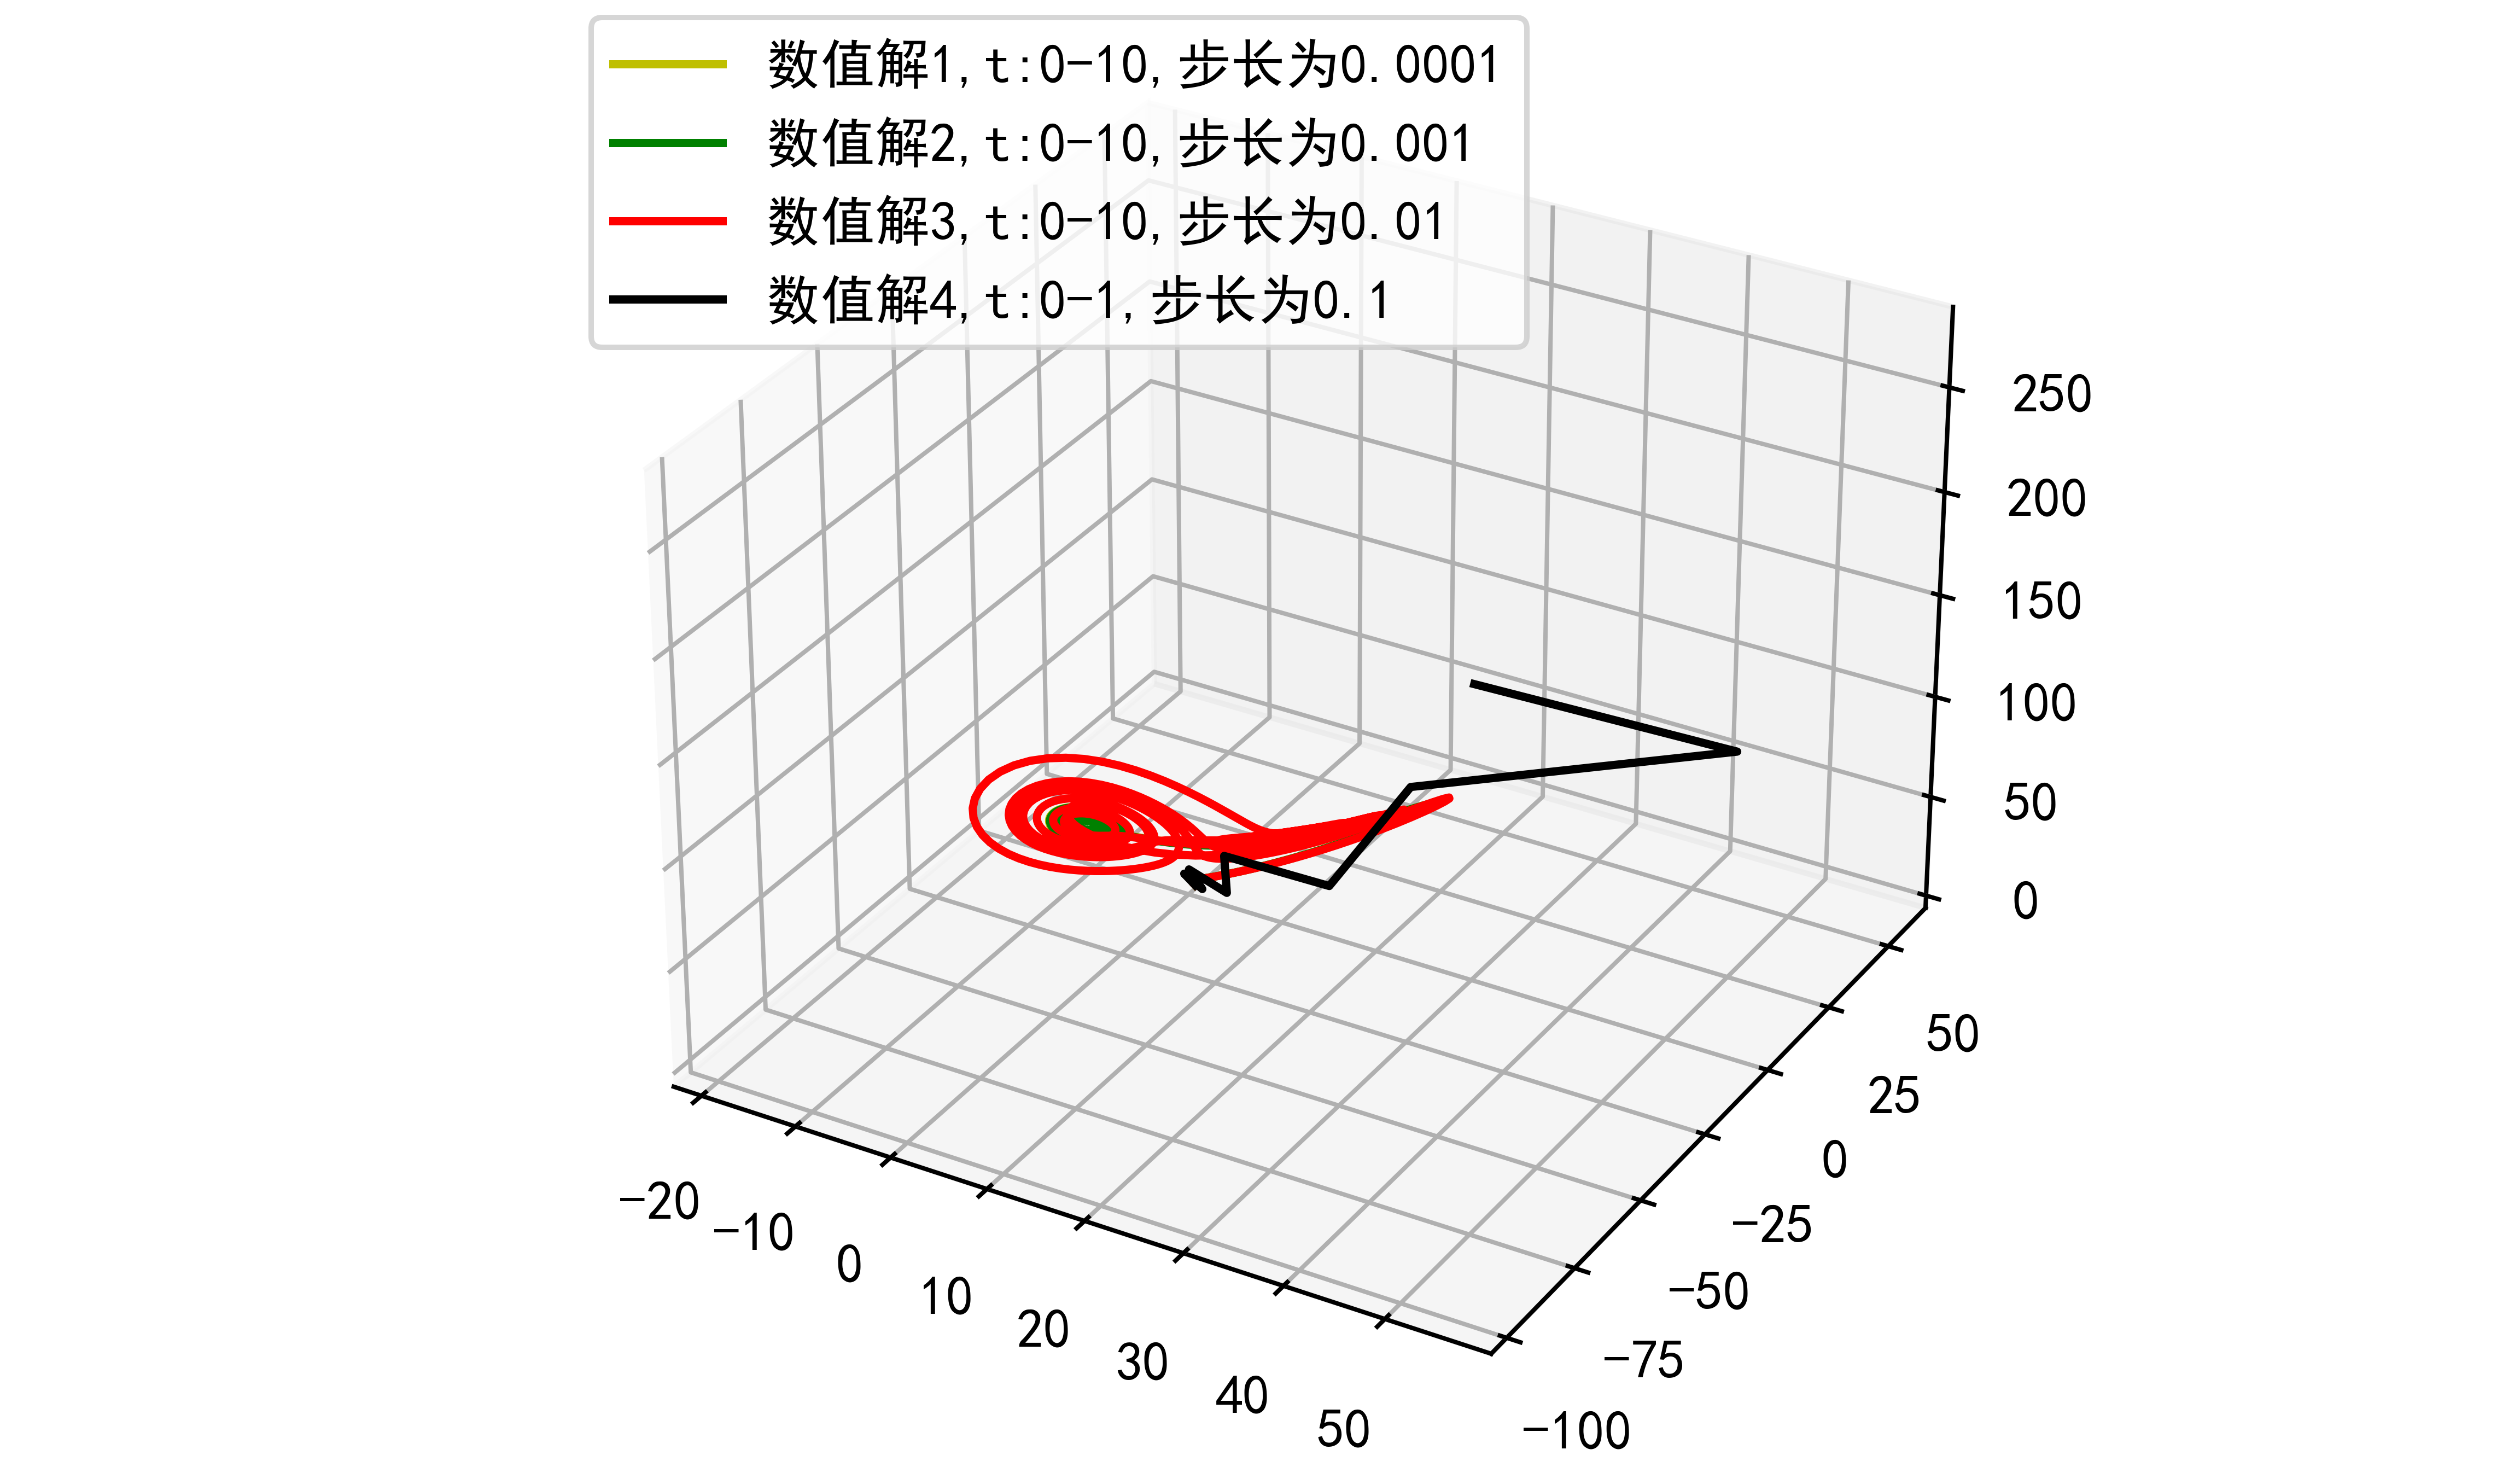
\includegraphics[scale=0.8]{35}
    \caption{起始点为(1,-1,1)}
\end{figure}

\begin{figure}[h]
    \begin{minipage}{0.48\linewidth}
    \centering
    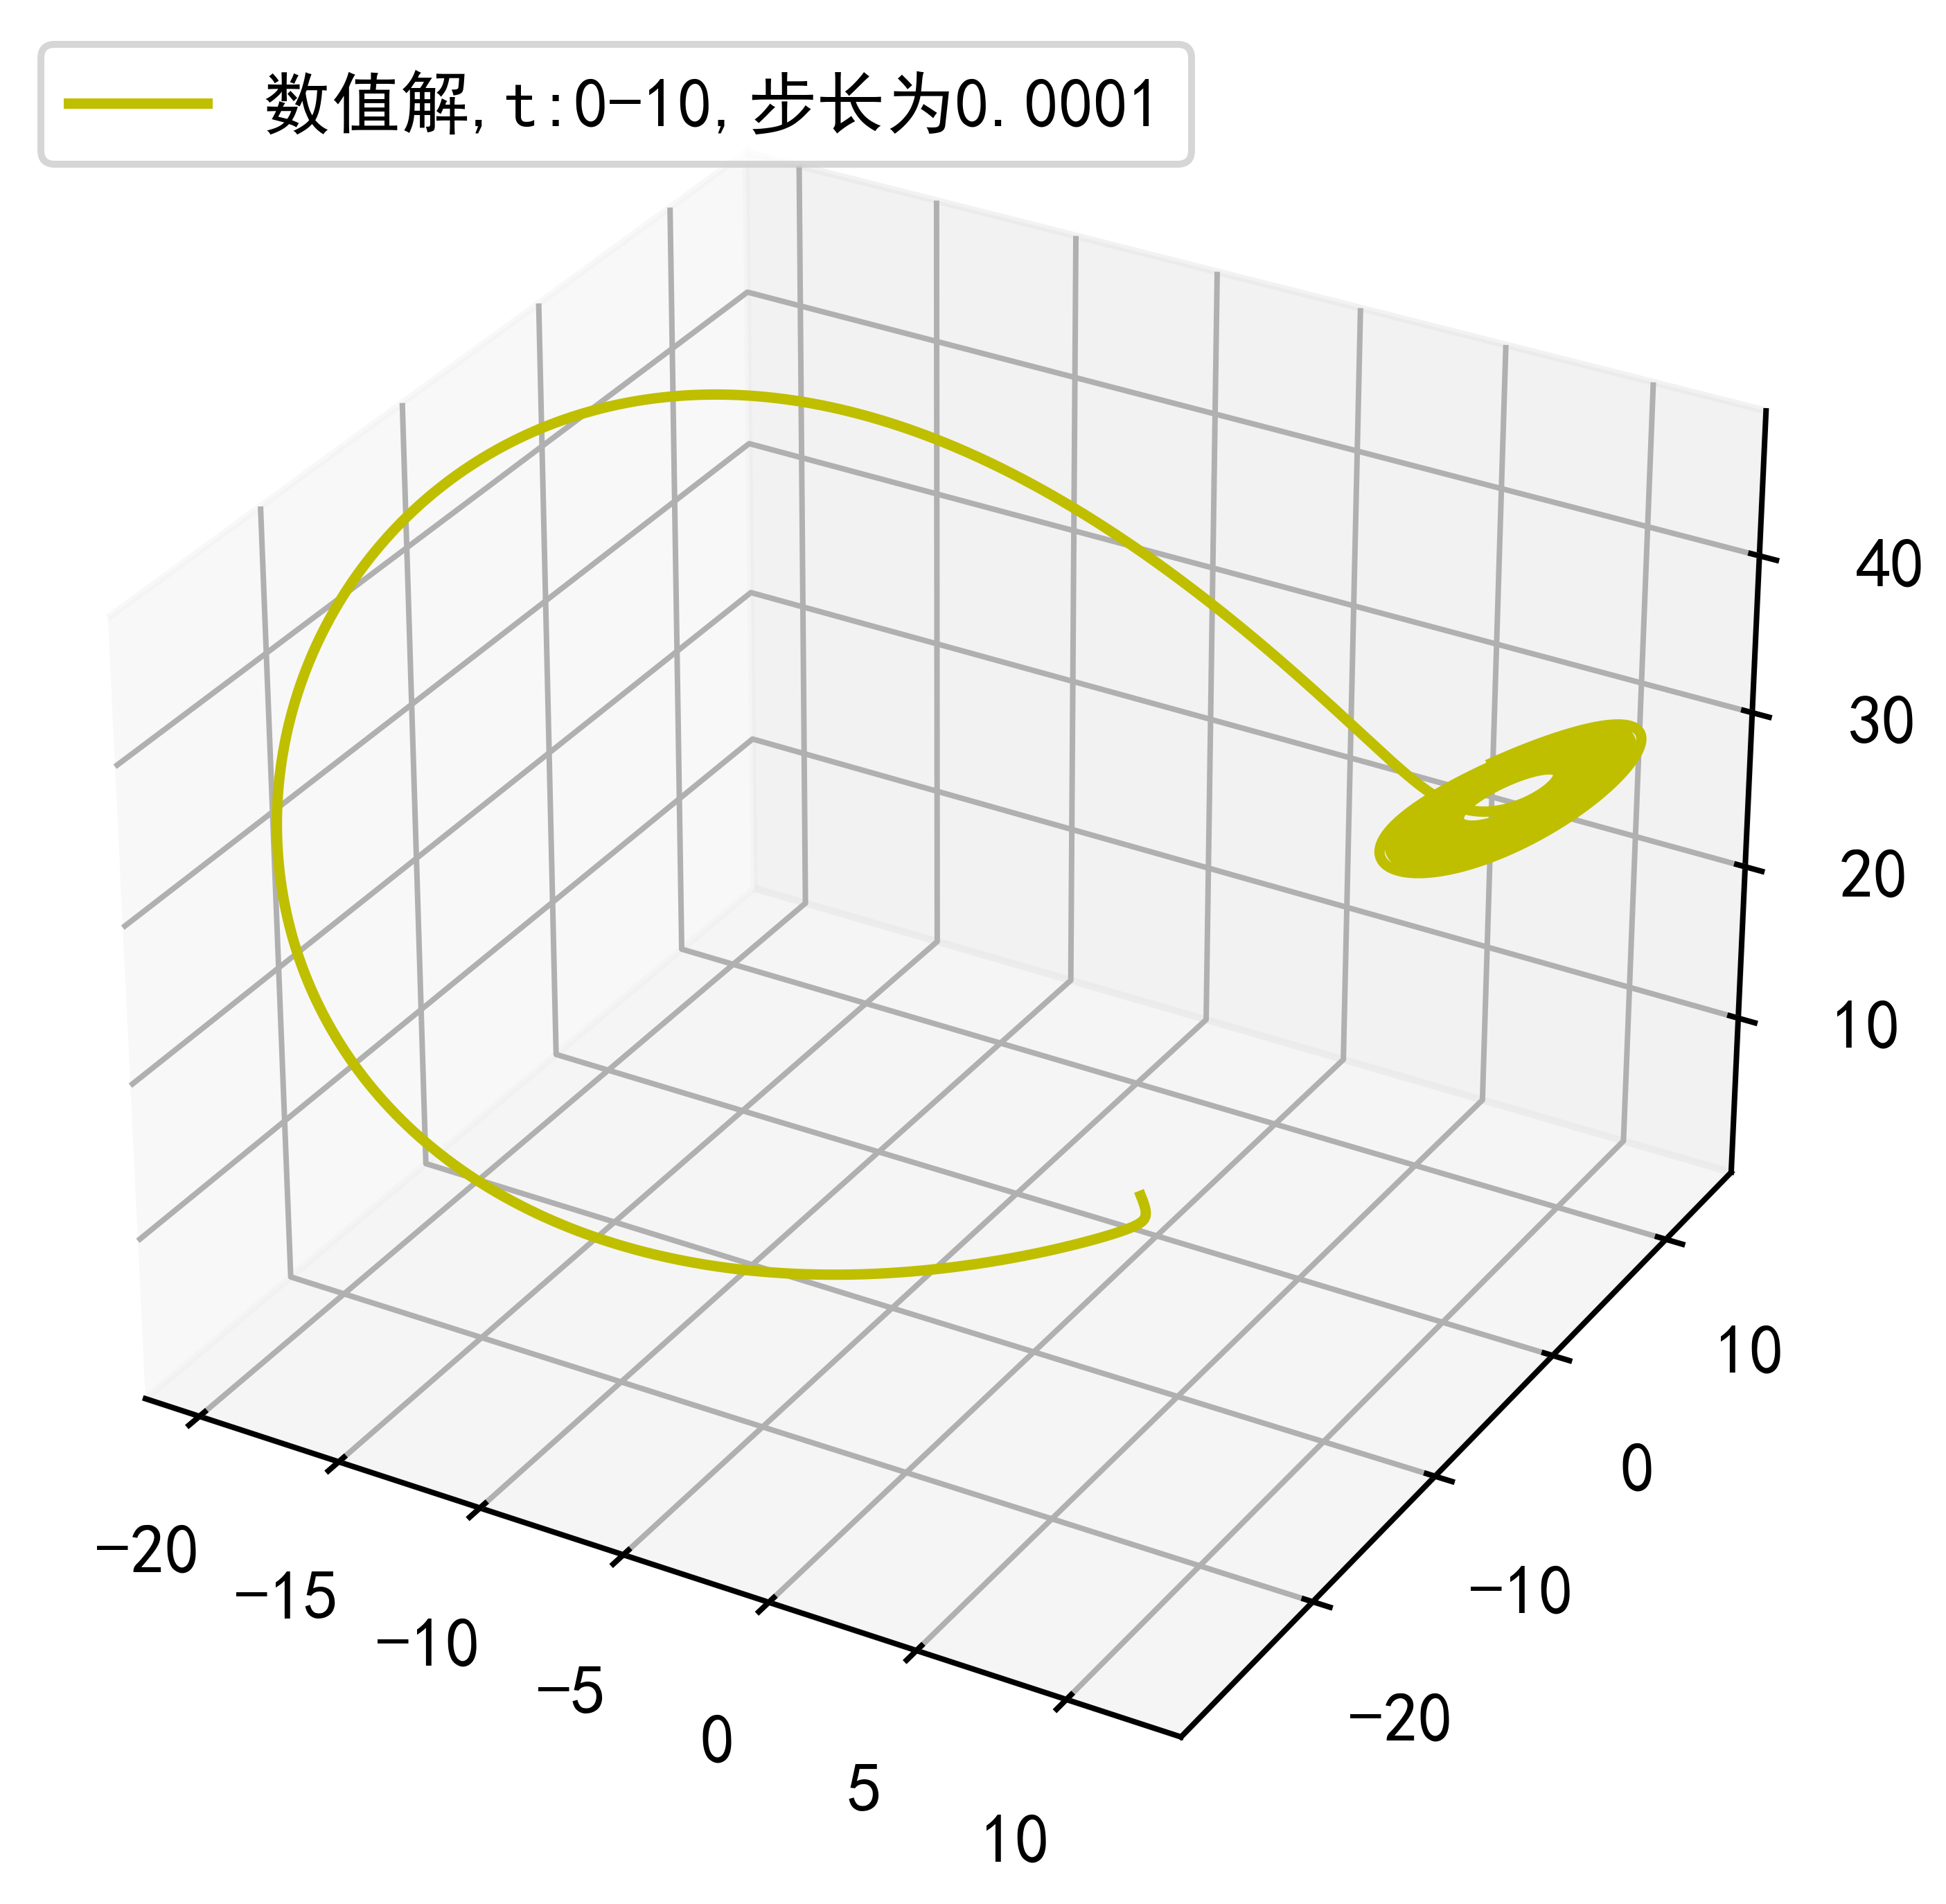
\includegraphics[scale=0.65]{41}
    \caption{起始点为(-1,1,1)}
    \end{minipage}
    \begin{minipage}{0.48\linewidth}
    \centering
    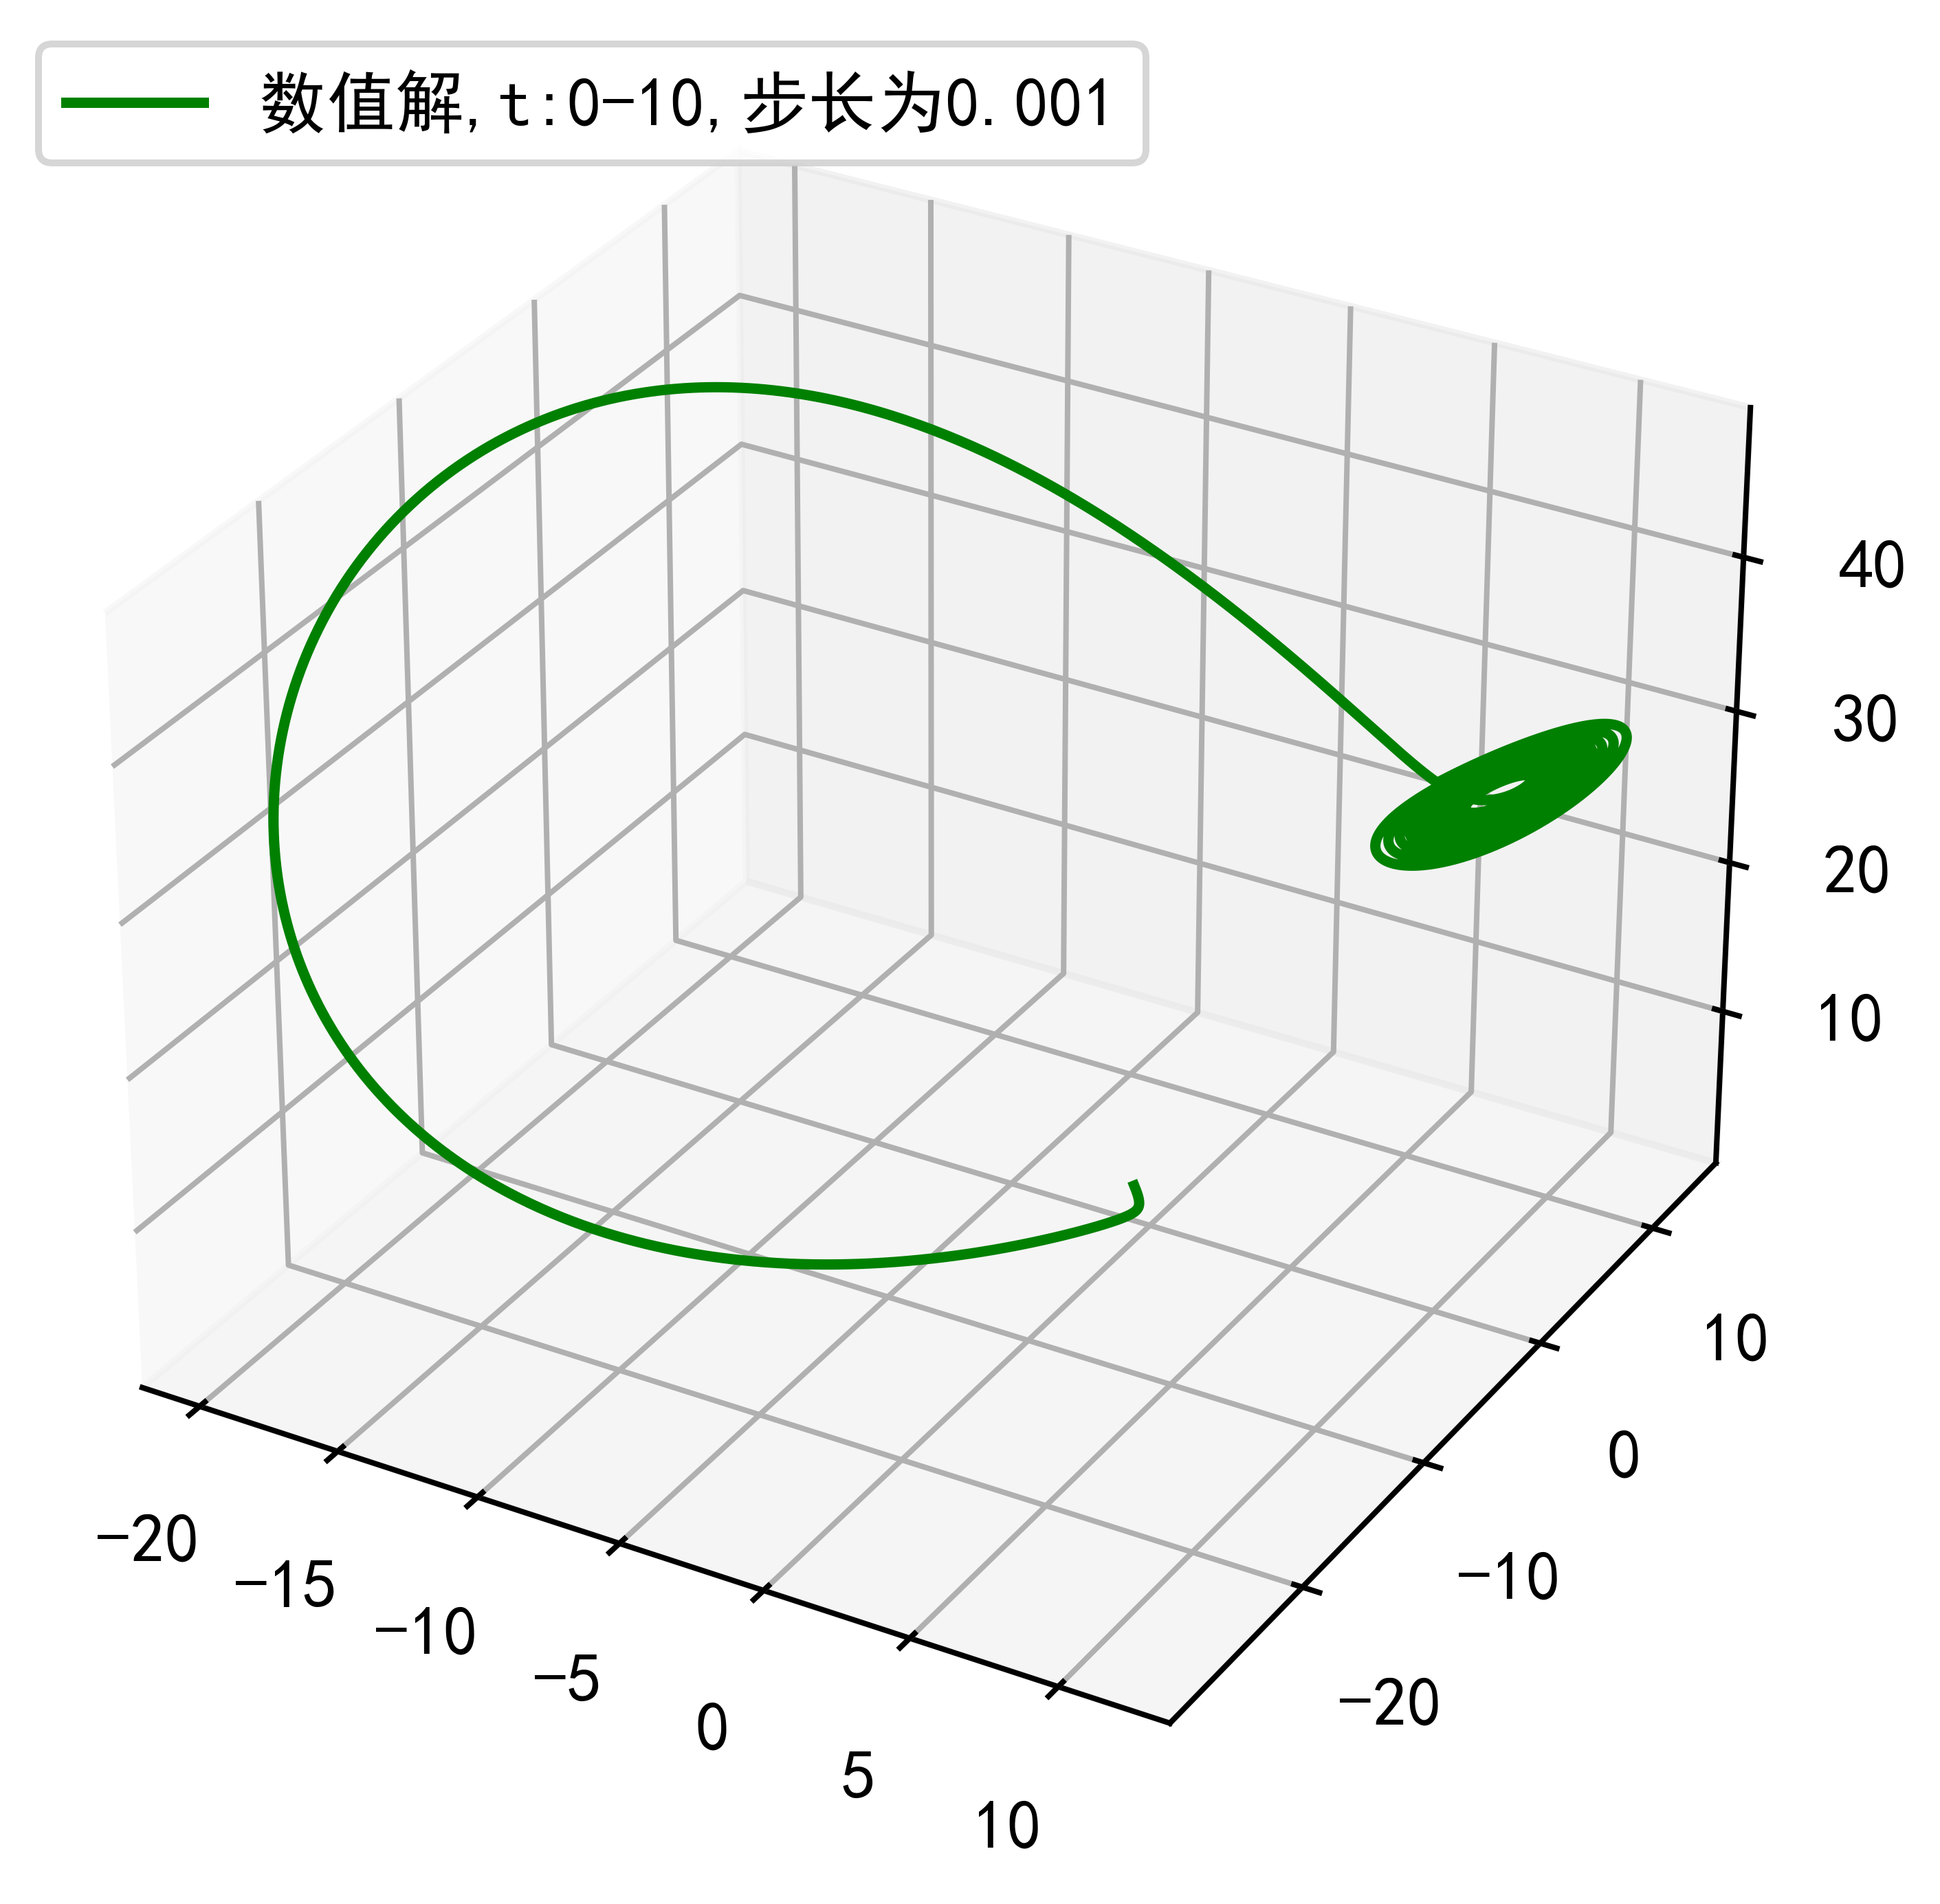
\includegraphics[scale=0.65]{42}
    \caption{起始点为(-1,1,1)}
    \end{minipage}
\end{figure}
\begin{figure}[h]
    \begin{minipage}[h]{0.48\linewidth}
    \centering
    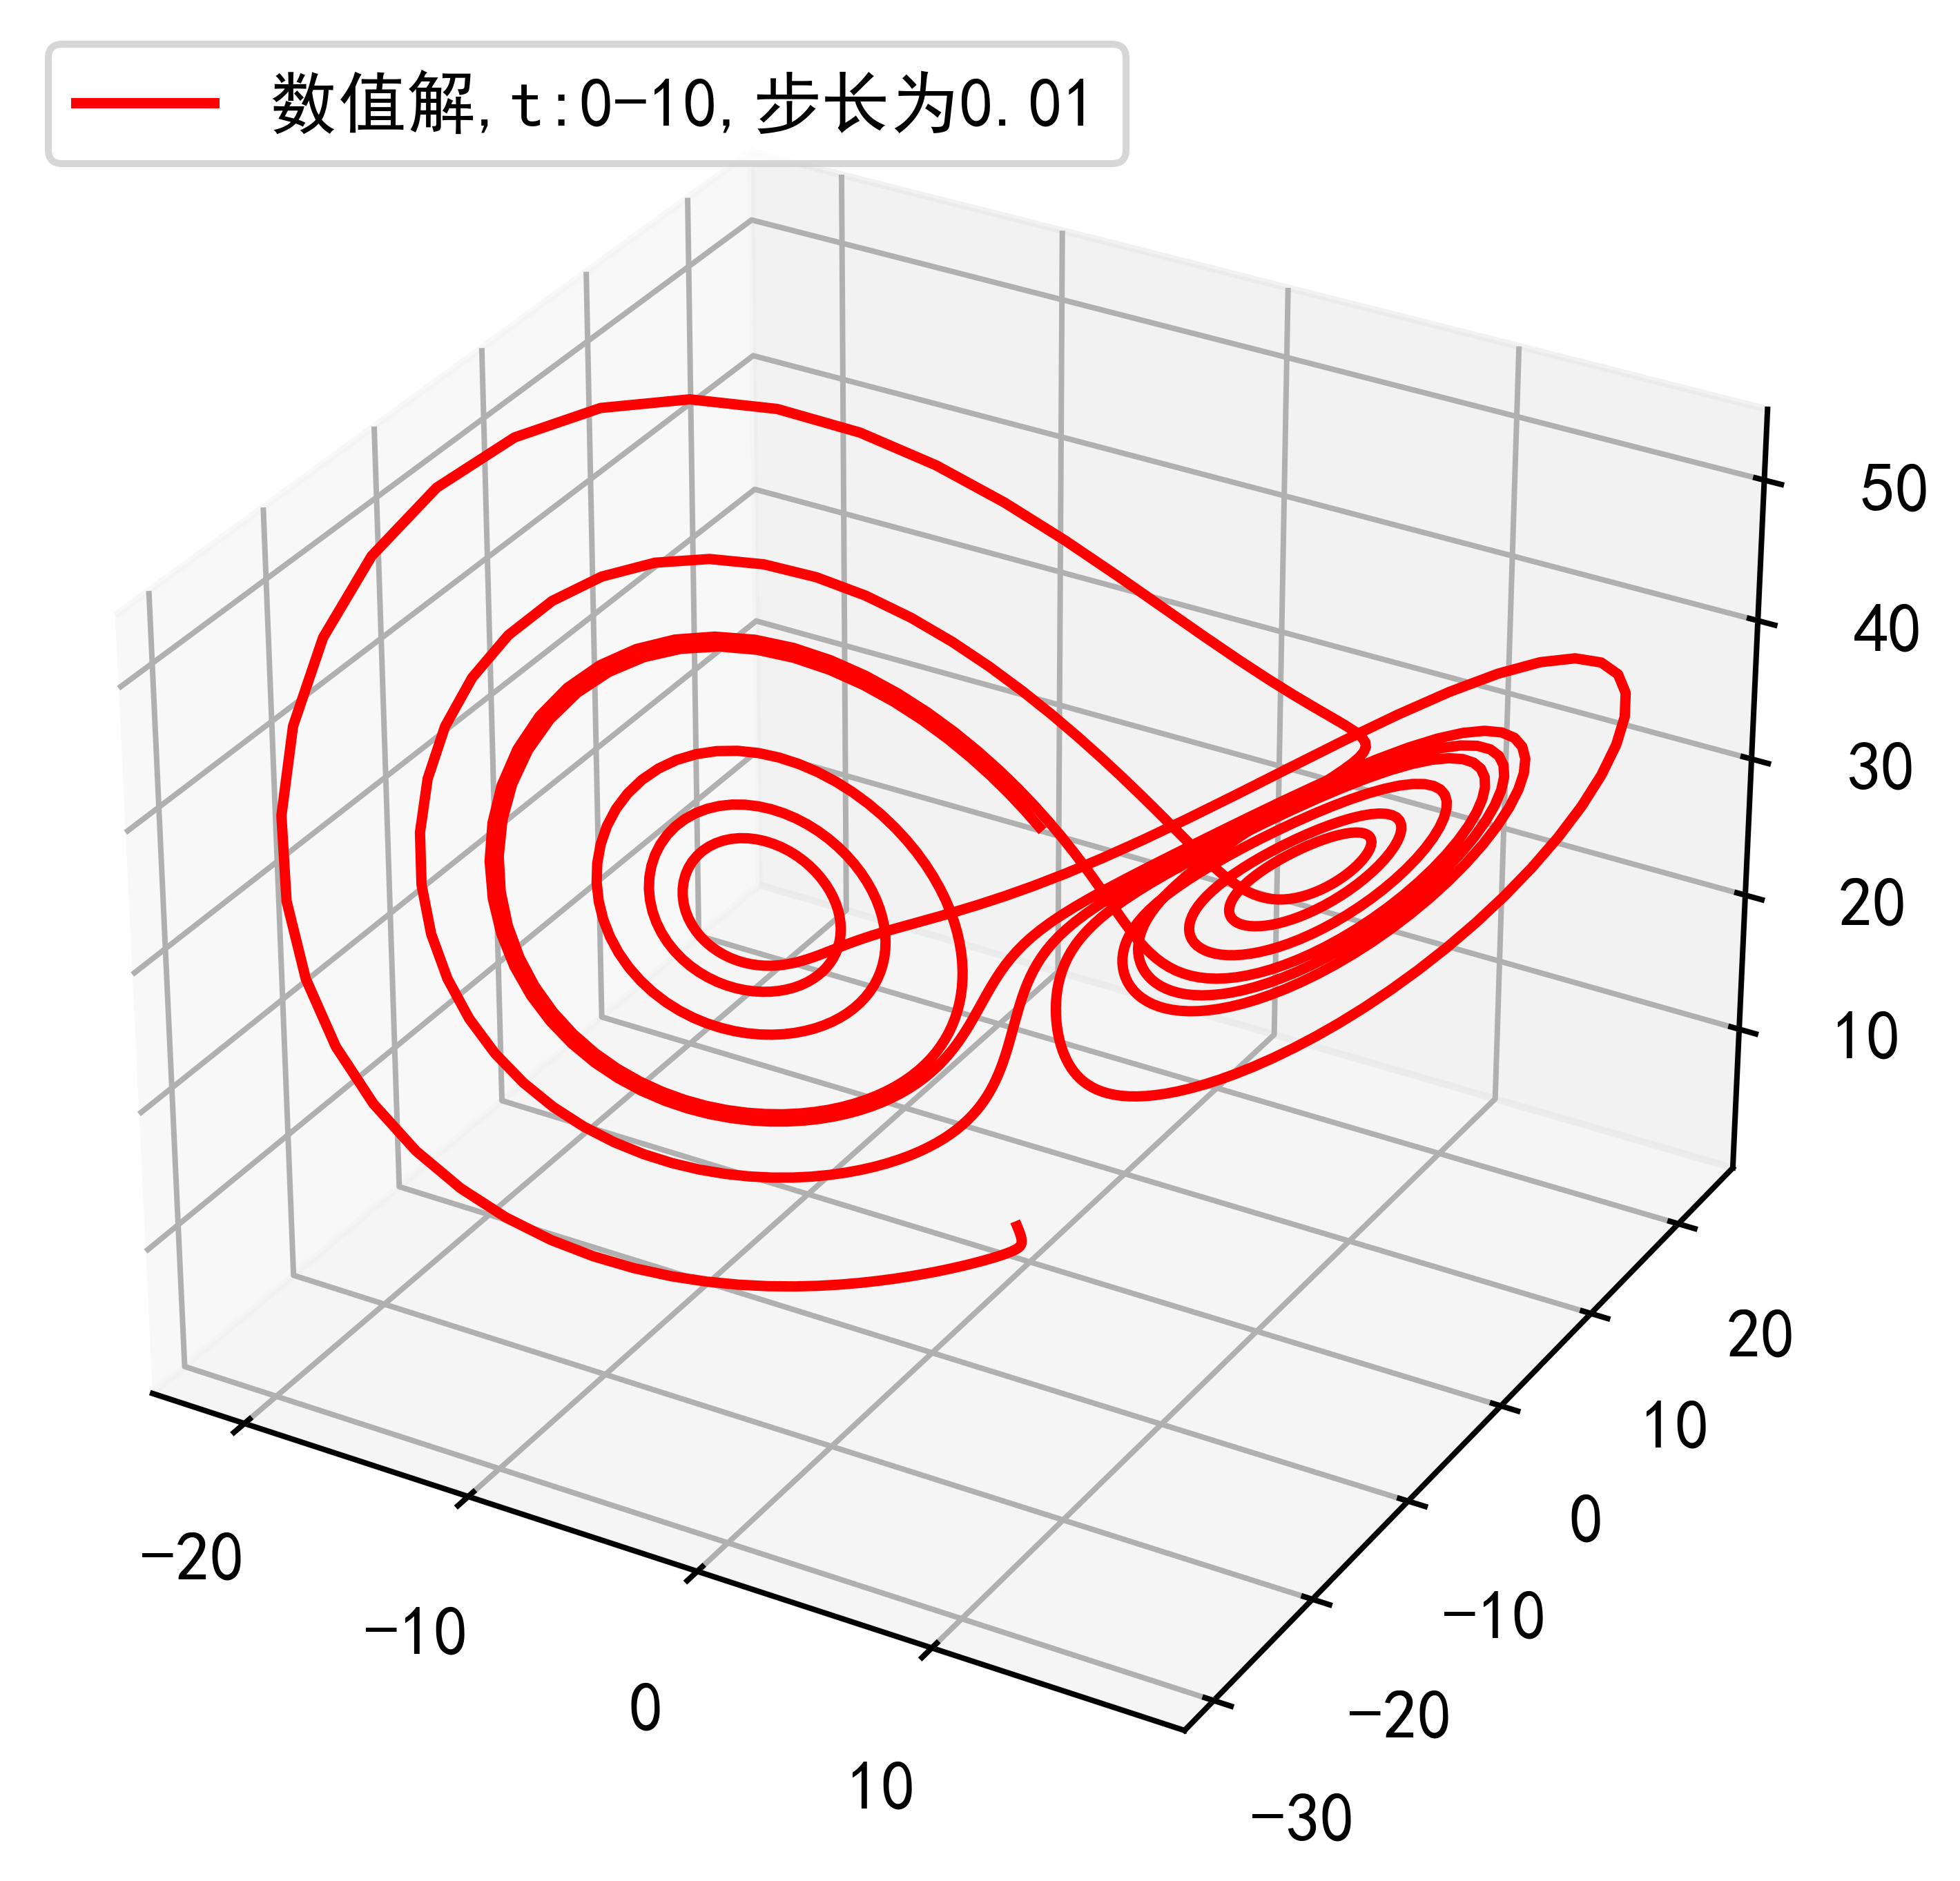
\includegraphics[scale=0.65]{43}
    \caption{起始点为(-1,1,1)}
    \end{minipage}
    \begin{minipage}[h]{0.48\linewidth}
    \centering
    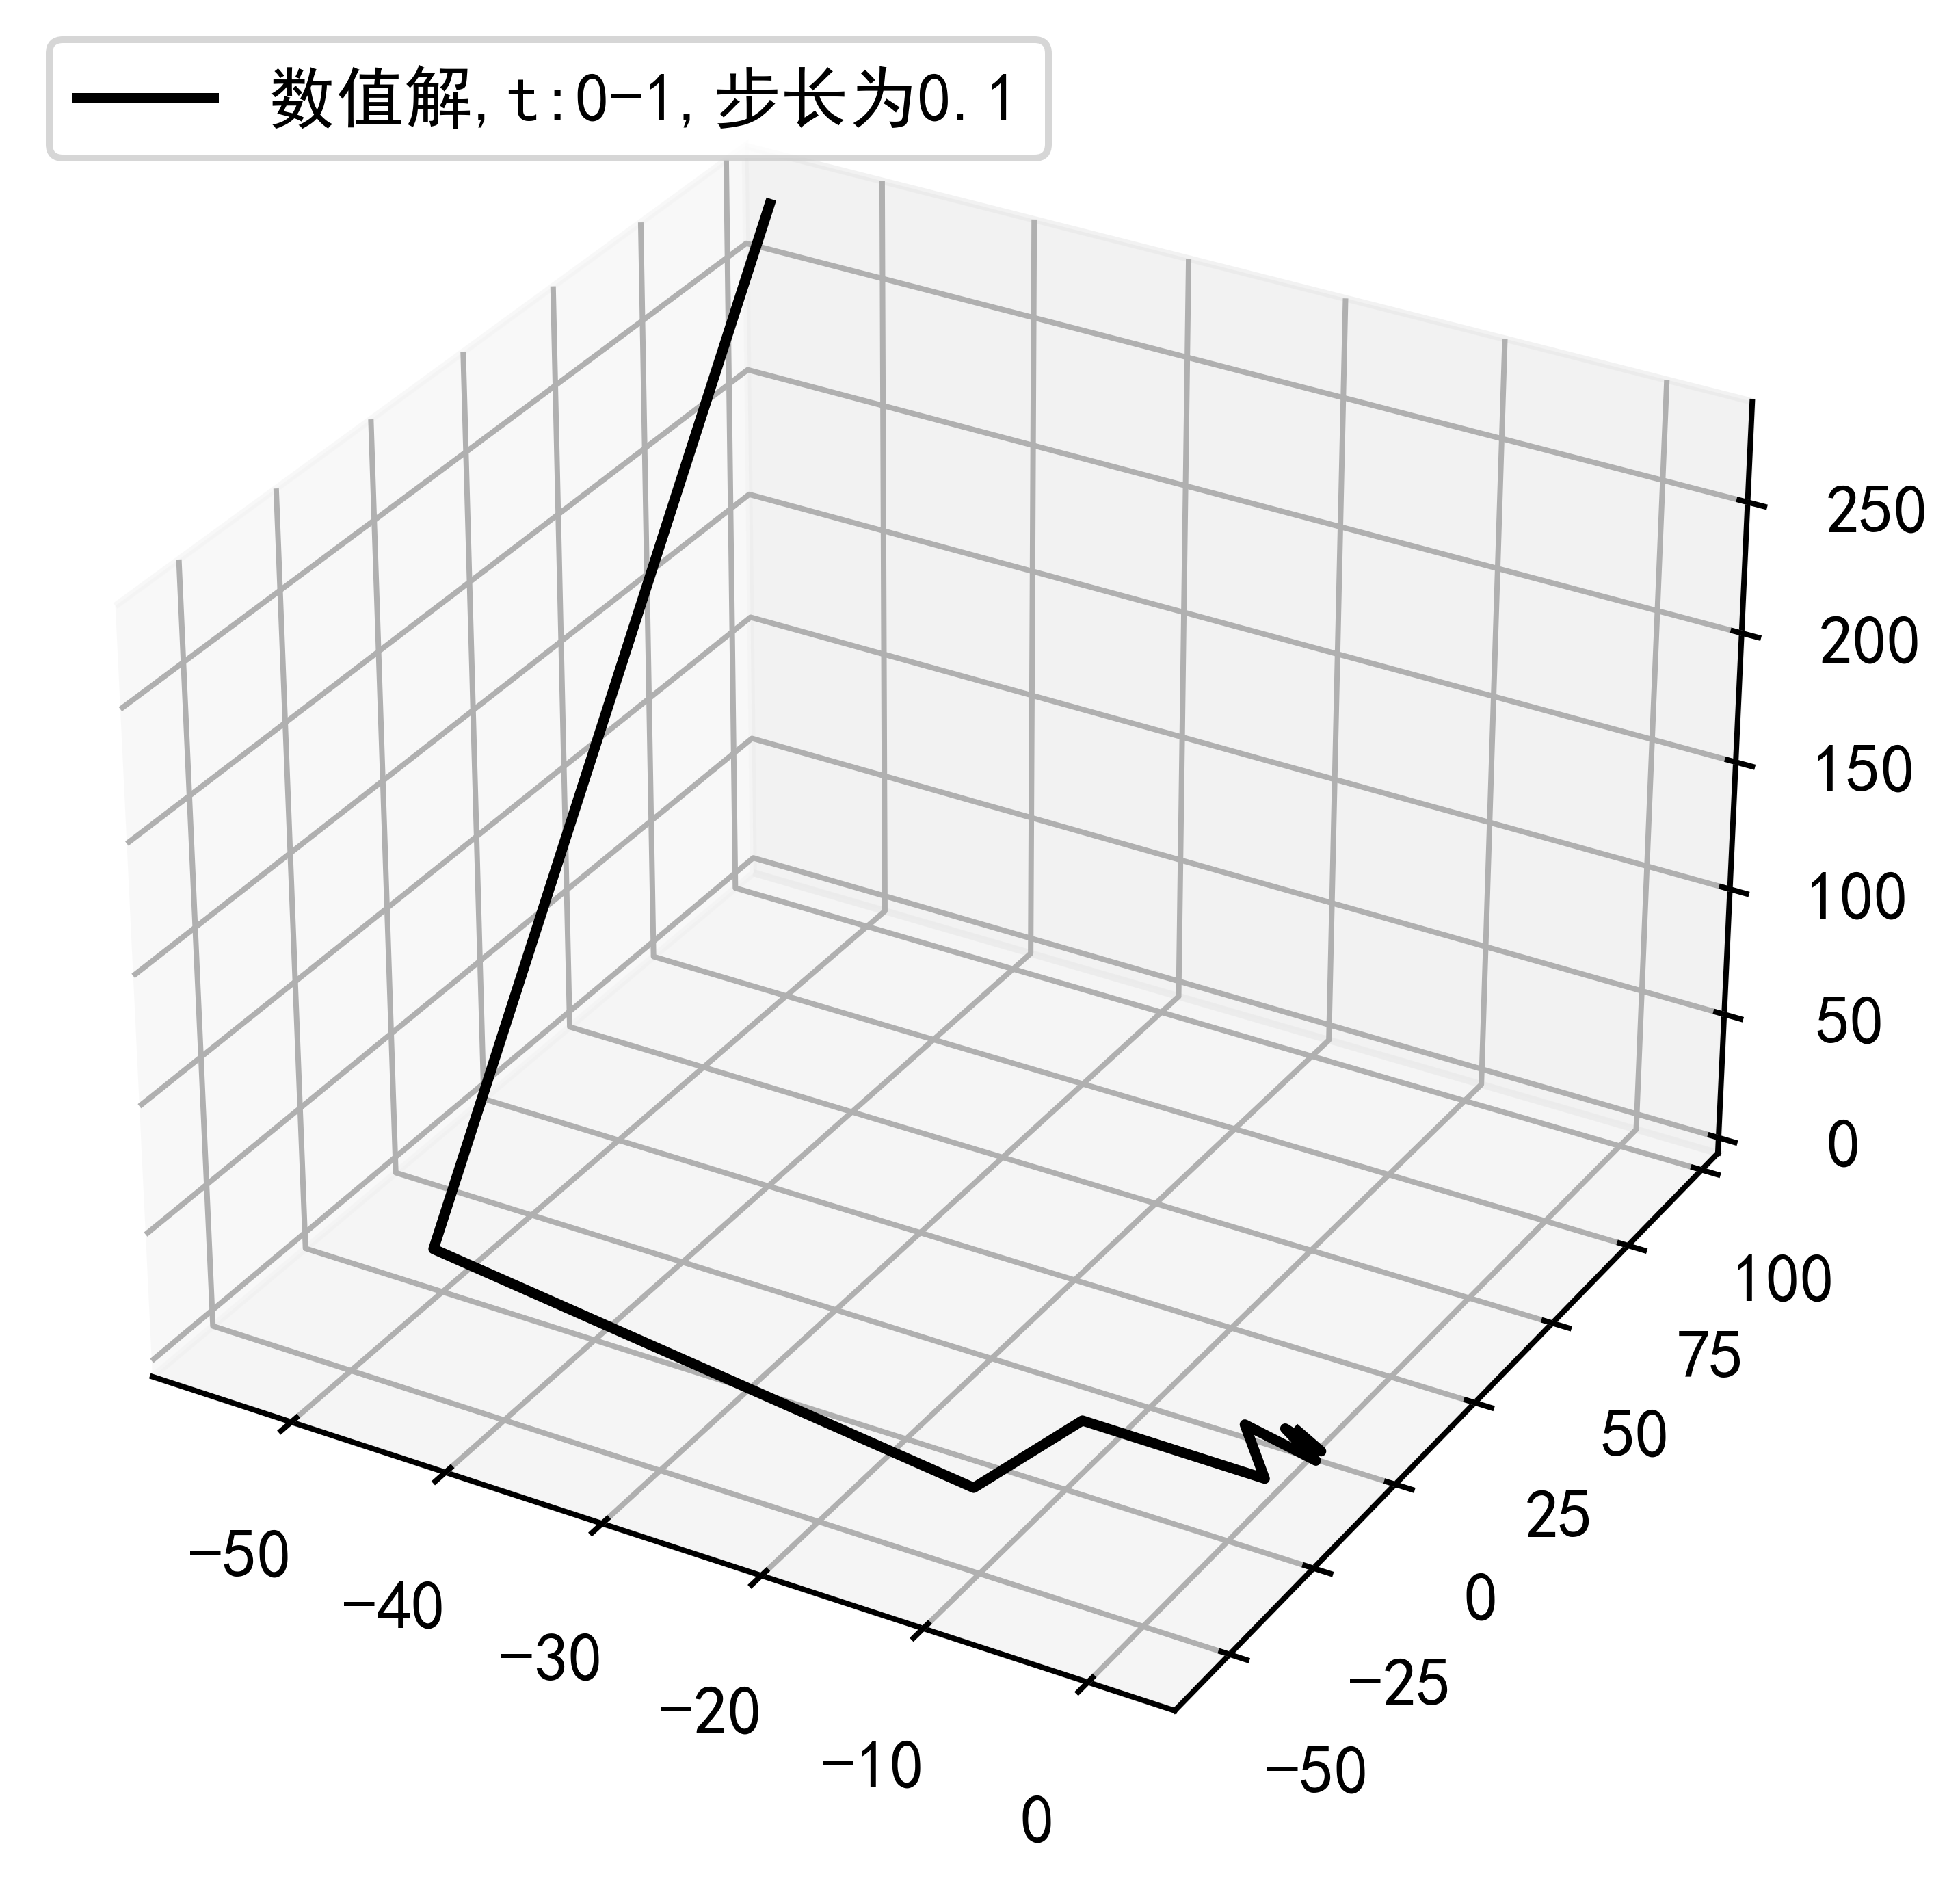
\includegraphics[scale=0.65]{44}
    \caption{起始点为(-1,1,1)}
    \end{minipage}
\end{figure}
\begin{figure}[H]
    \centering
    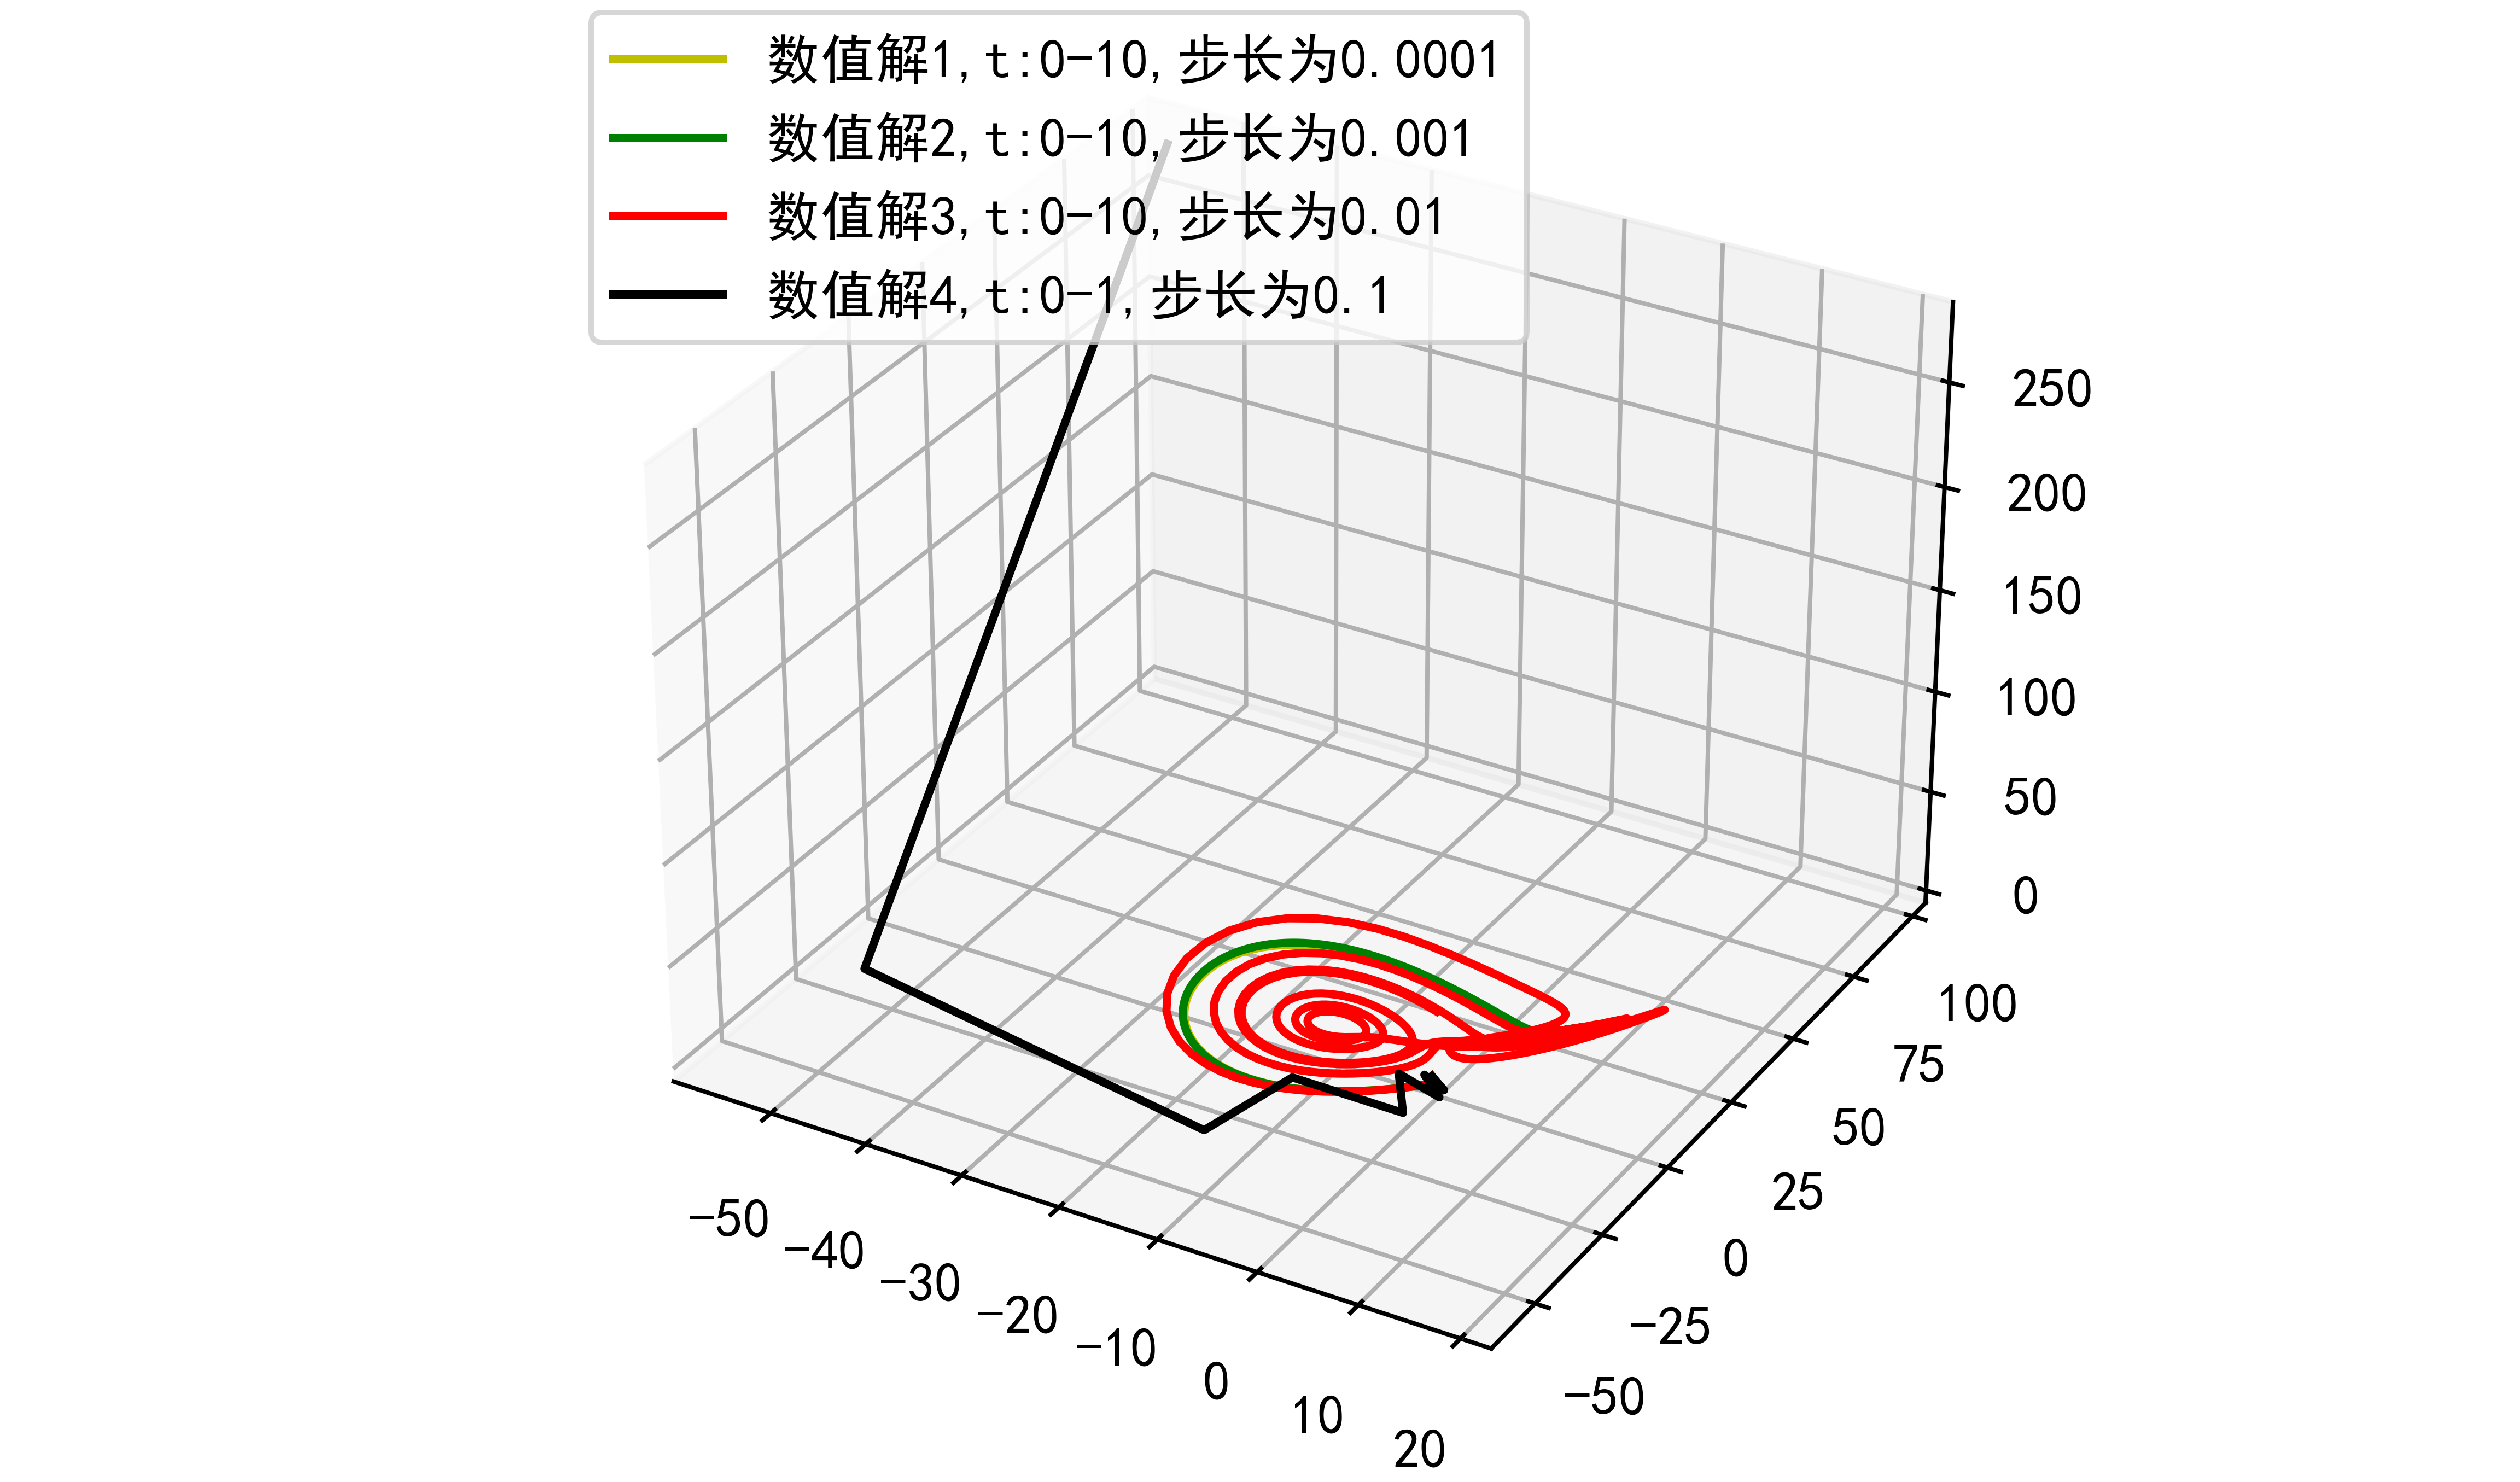
\includegraphics[scale=0.8]{45}
    \caption{起始点为(-1,1,1)}
\end{figure}

\begin{figure}[h]
    \begin{minipage}{0.48\linewidth}
    \centering
    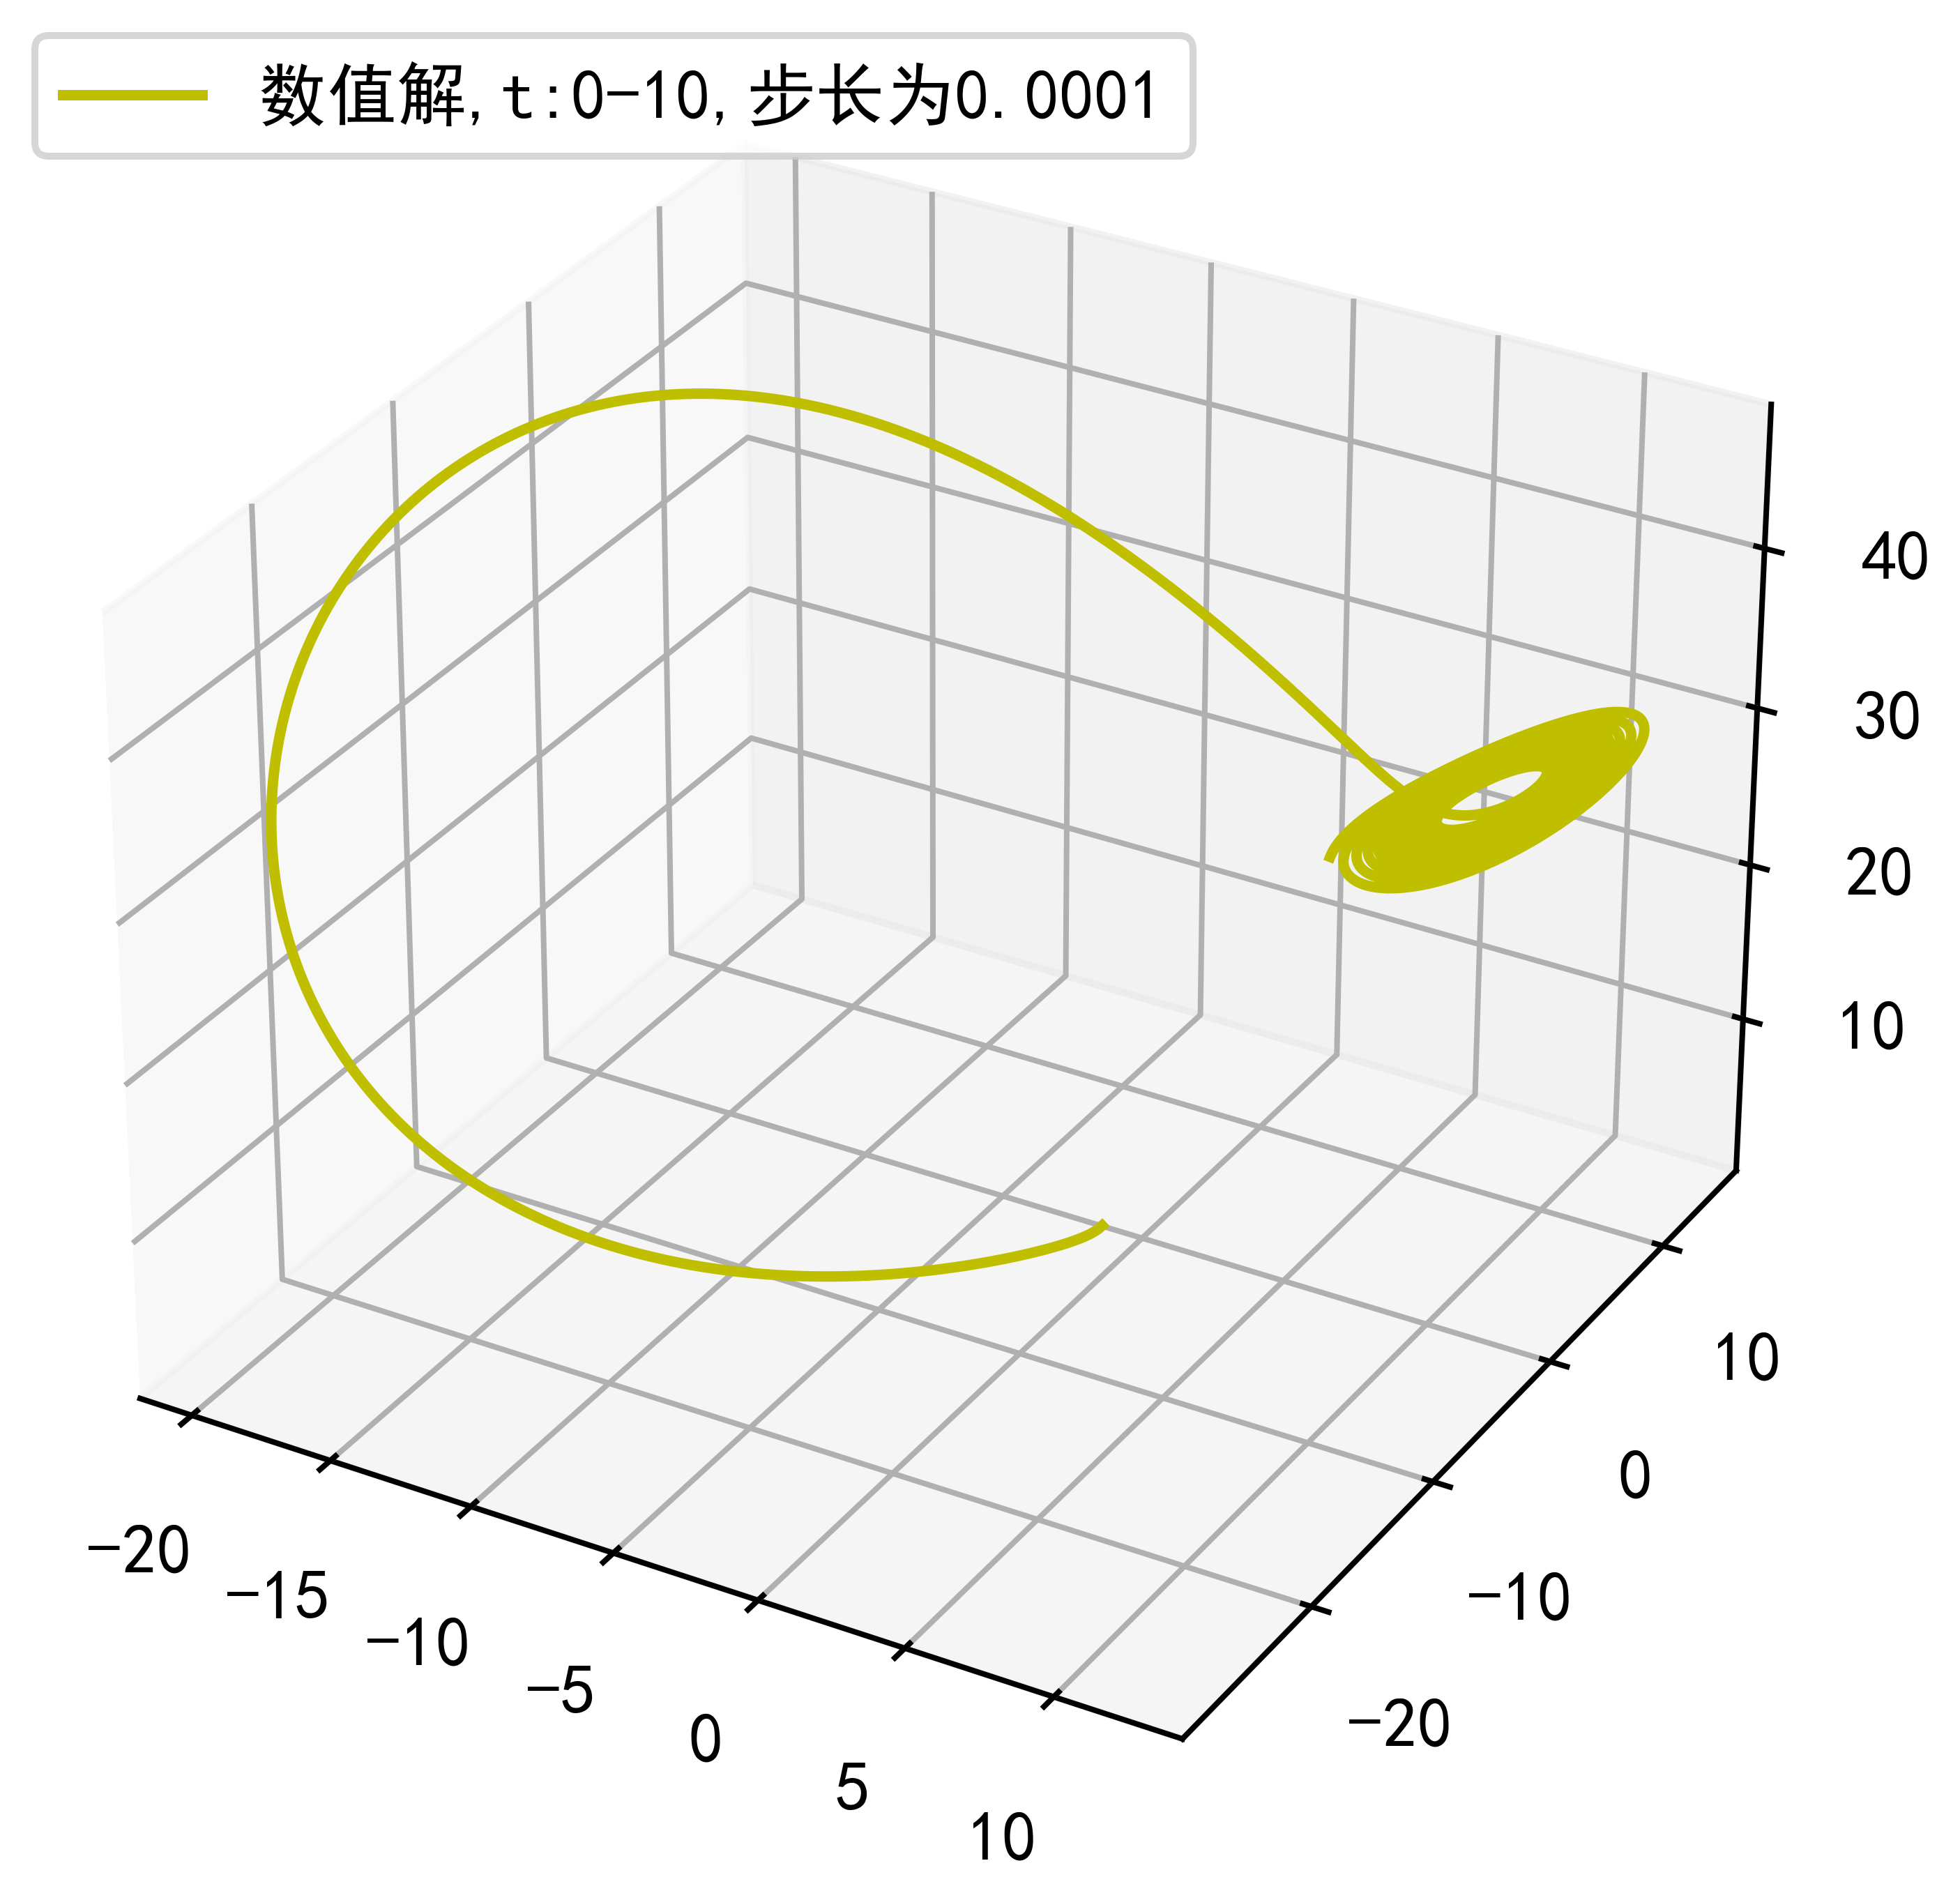
\includegraphics[scale=0.65]{51}
    \caption{起始点为(-1,-1,1)}
    \end{minipage}
    \begin{minipage}{0.48\linewidth}
    \centering
    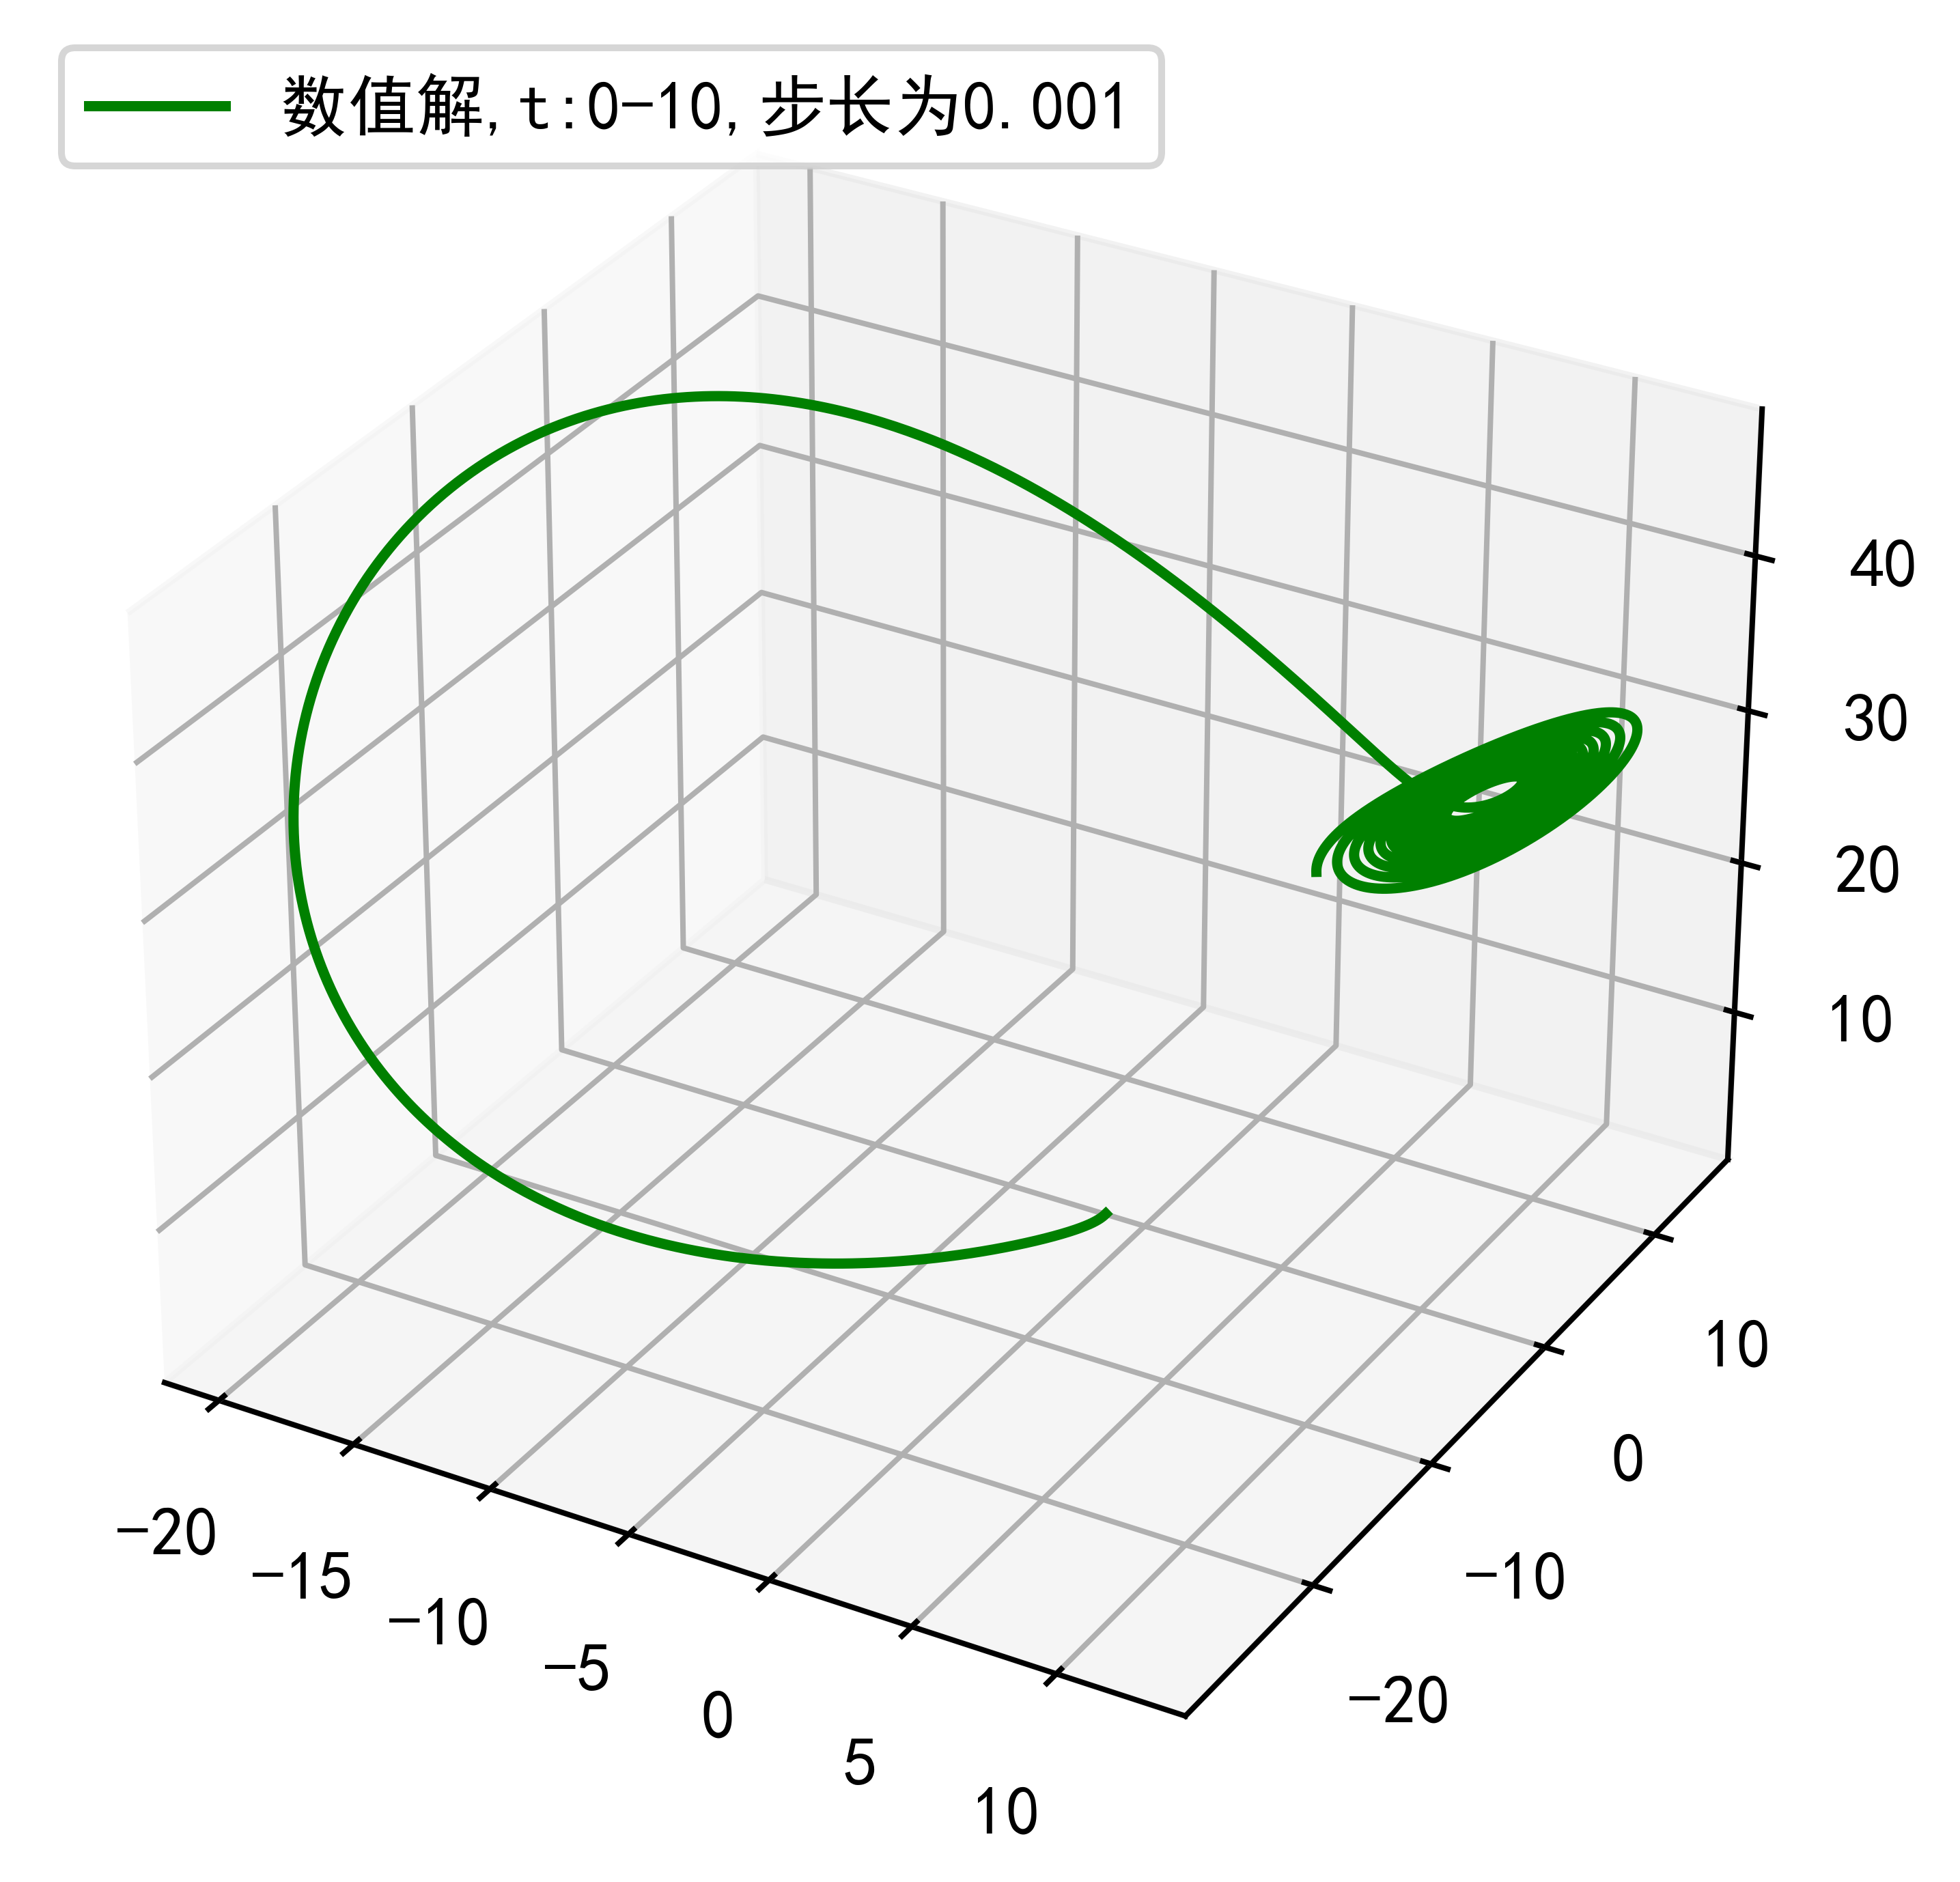
\includegraphics[scale=0.65]{52}
    \caption{起始点为(-1,-1,1)}
    \end{minipage}
\end{figure}
\begin{figure}[h]
    \begin{minipage}[h]{0.48\linewidth}
    \centering
    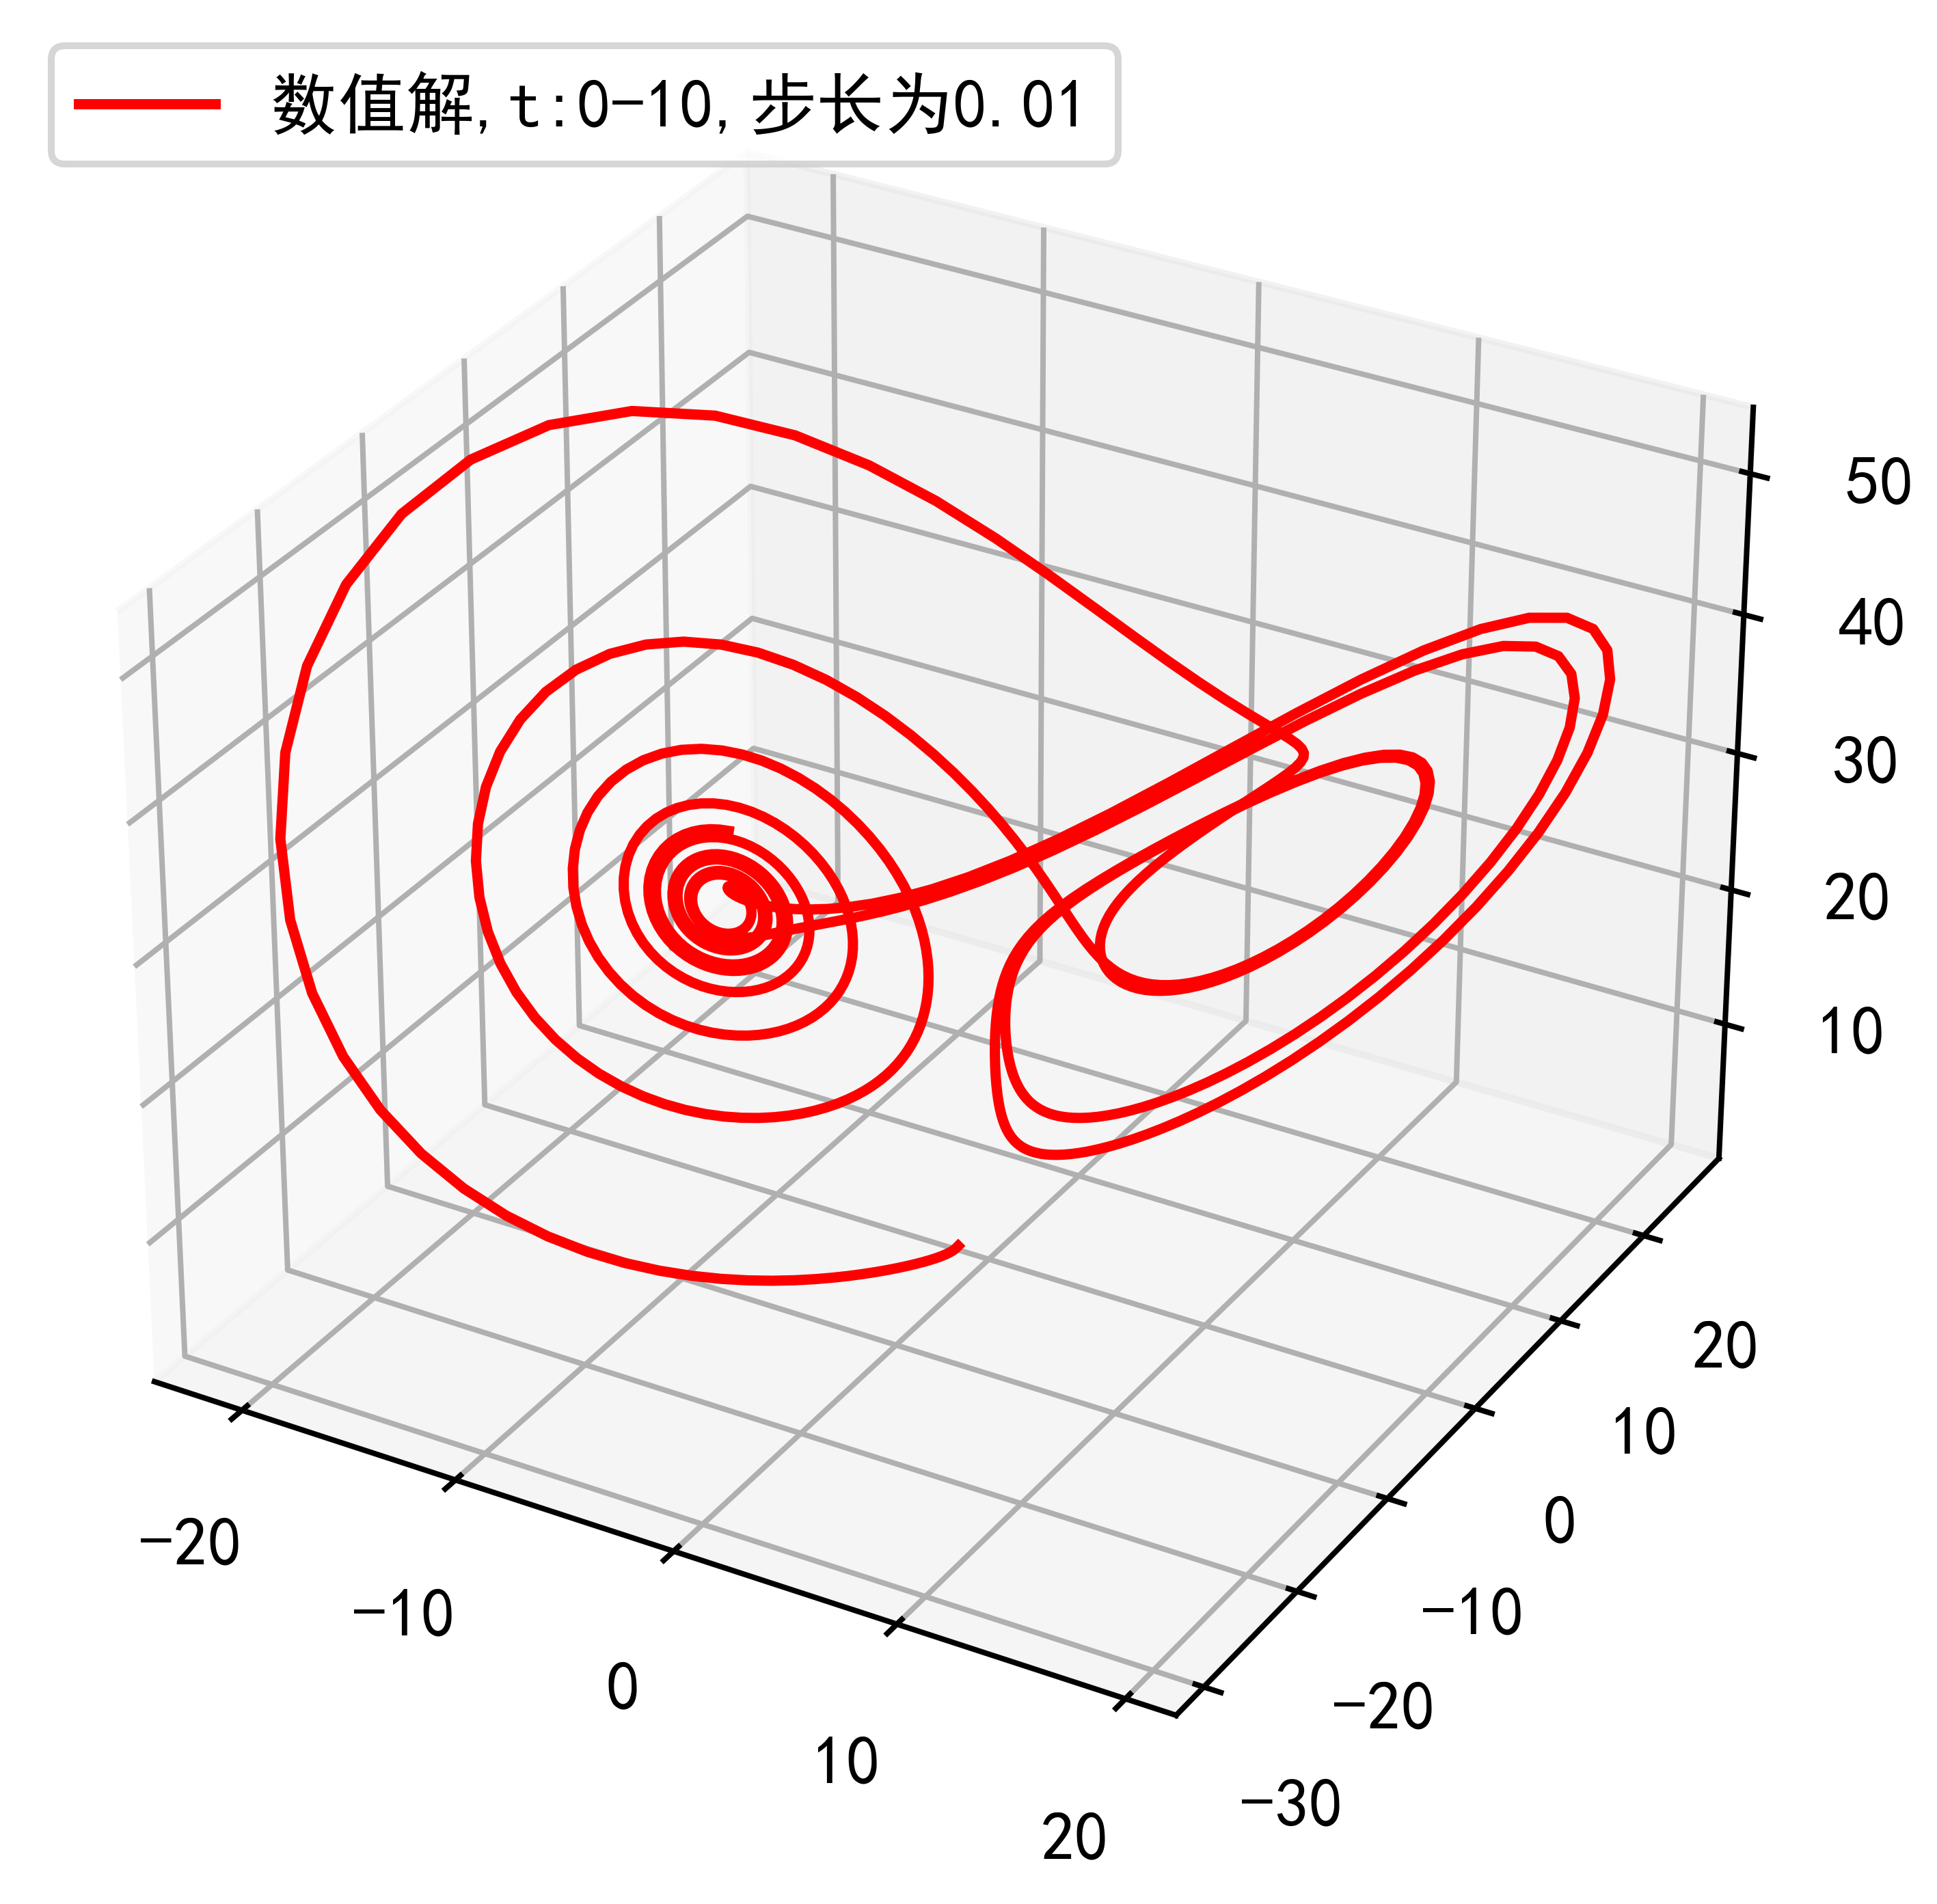
\includegraphics[scale=0.65]{53}
    \caption{起始点为(-1,-1,1)}
    \end{minipage}
    \begin{minipage}[h]{0.48\linewidth}
    \centering
    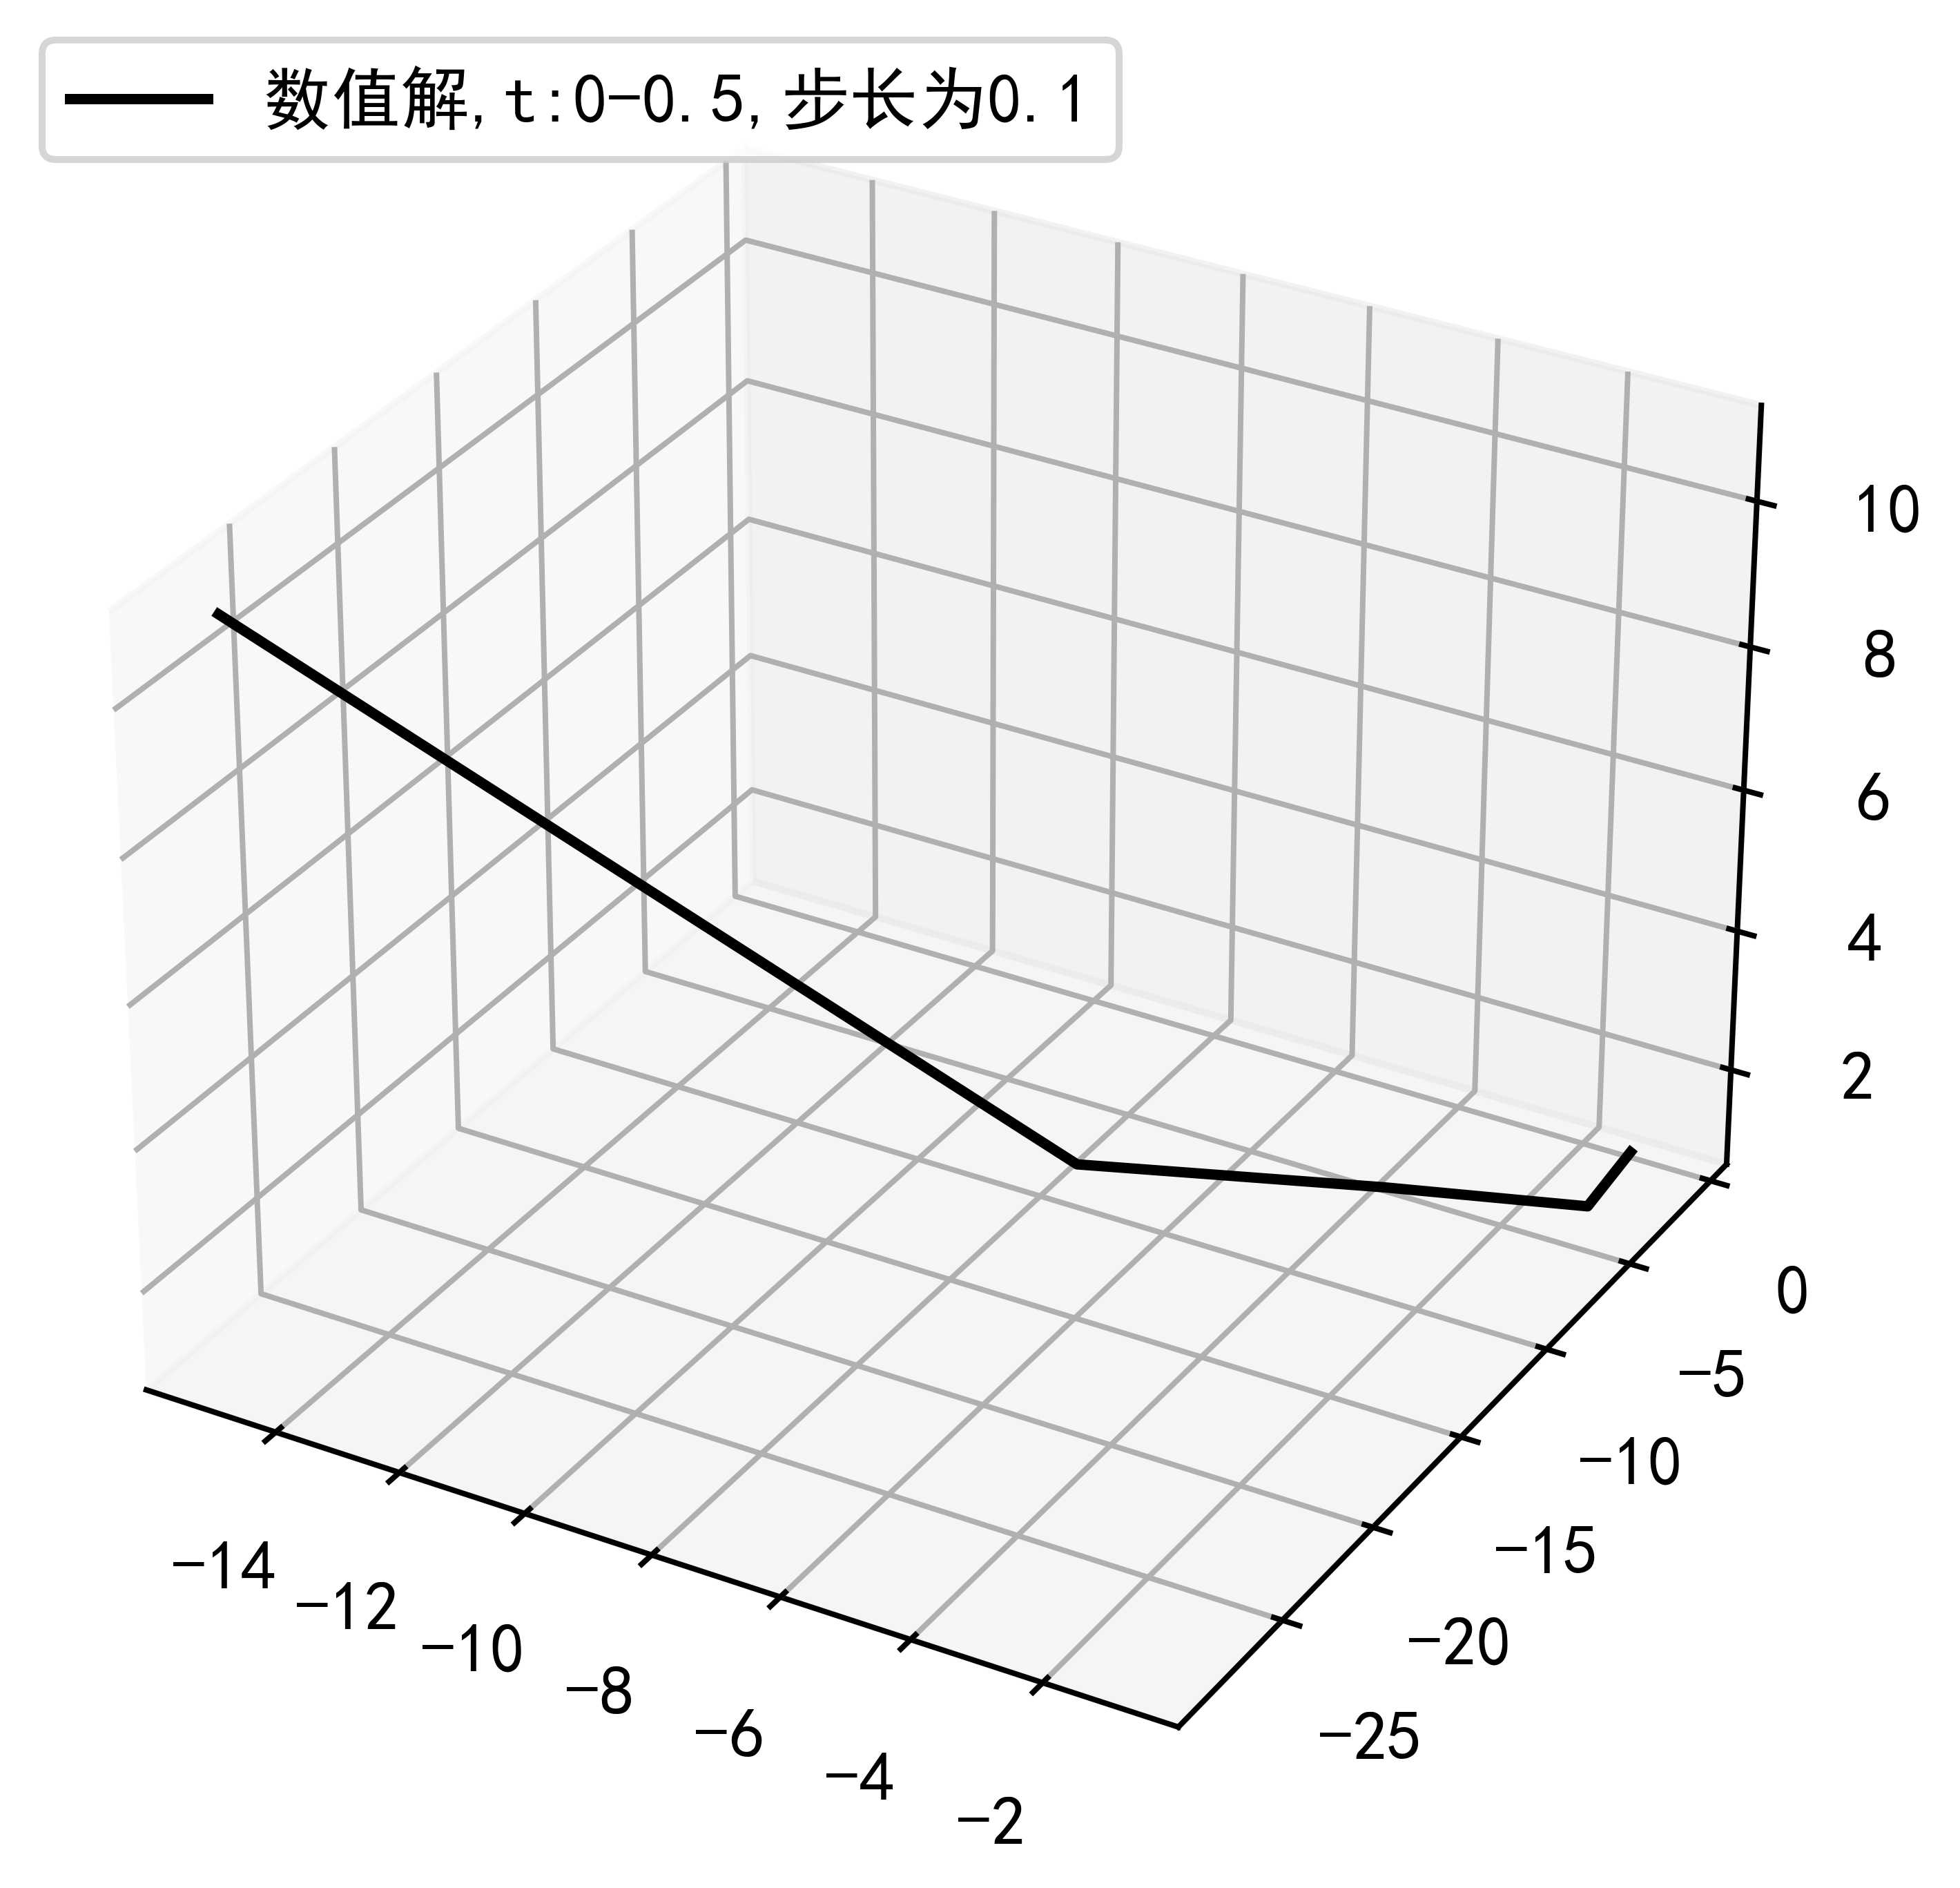
\includegraphics[scale=0.65]{54}
    \caption{起始点为(-1,-1,1)}
    \end{minipage}
\end{figure}
\begin{figure}[H]
    \centering
    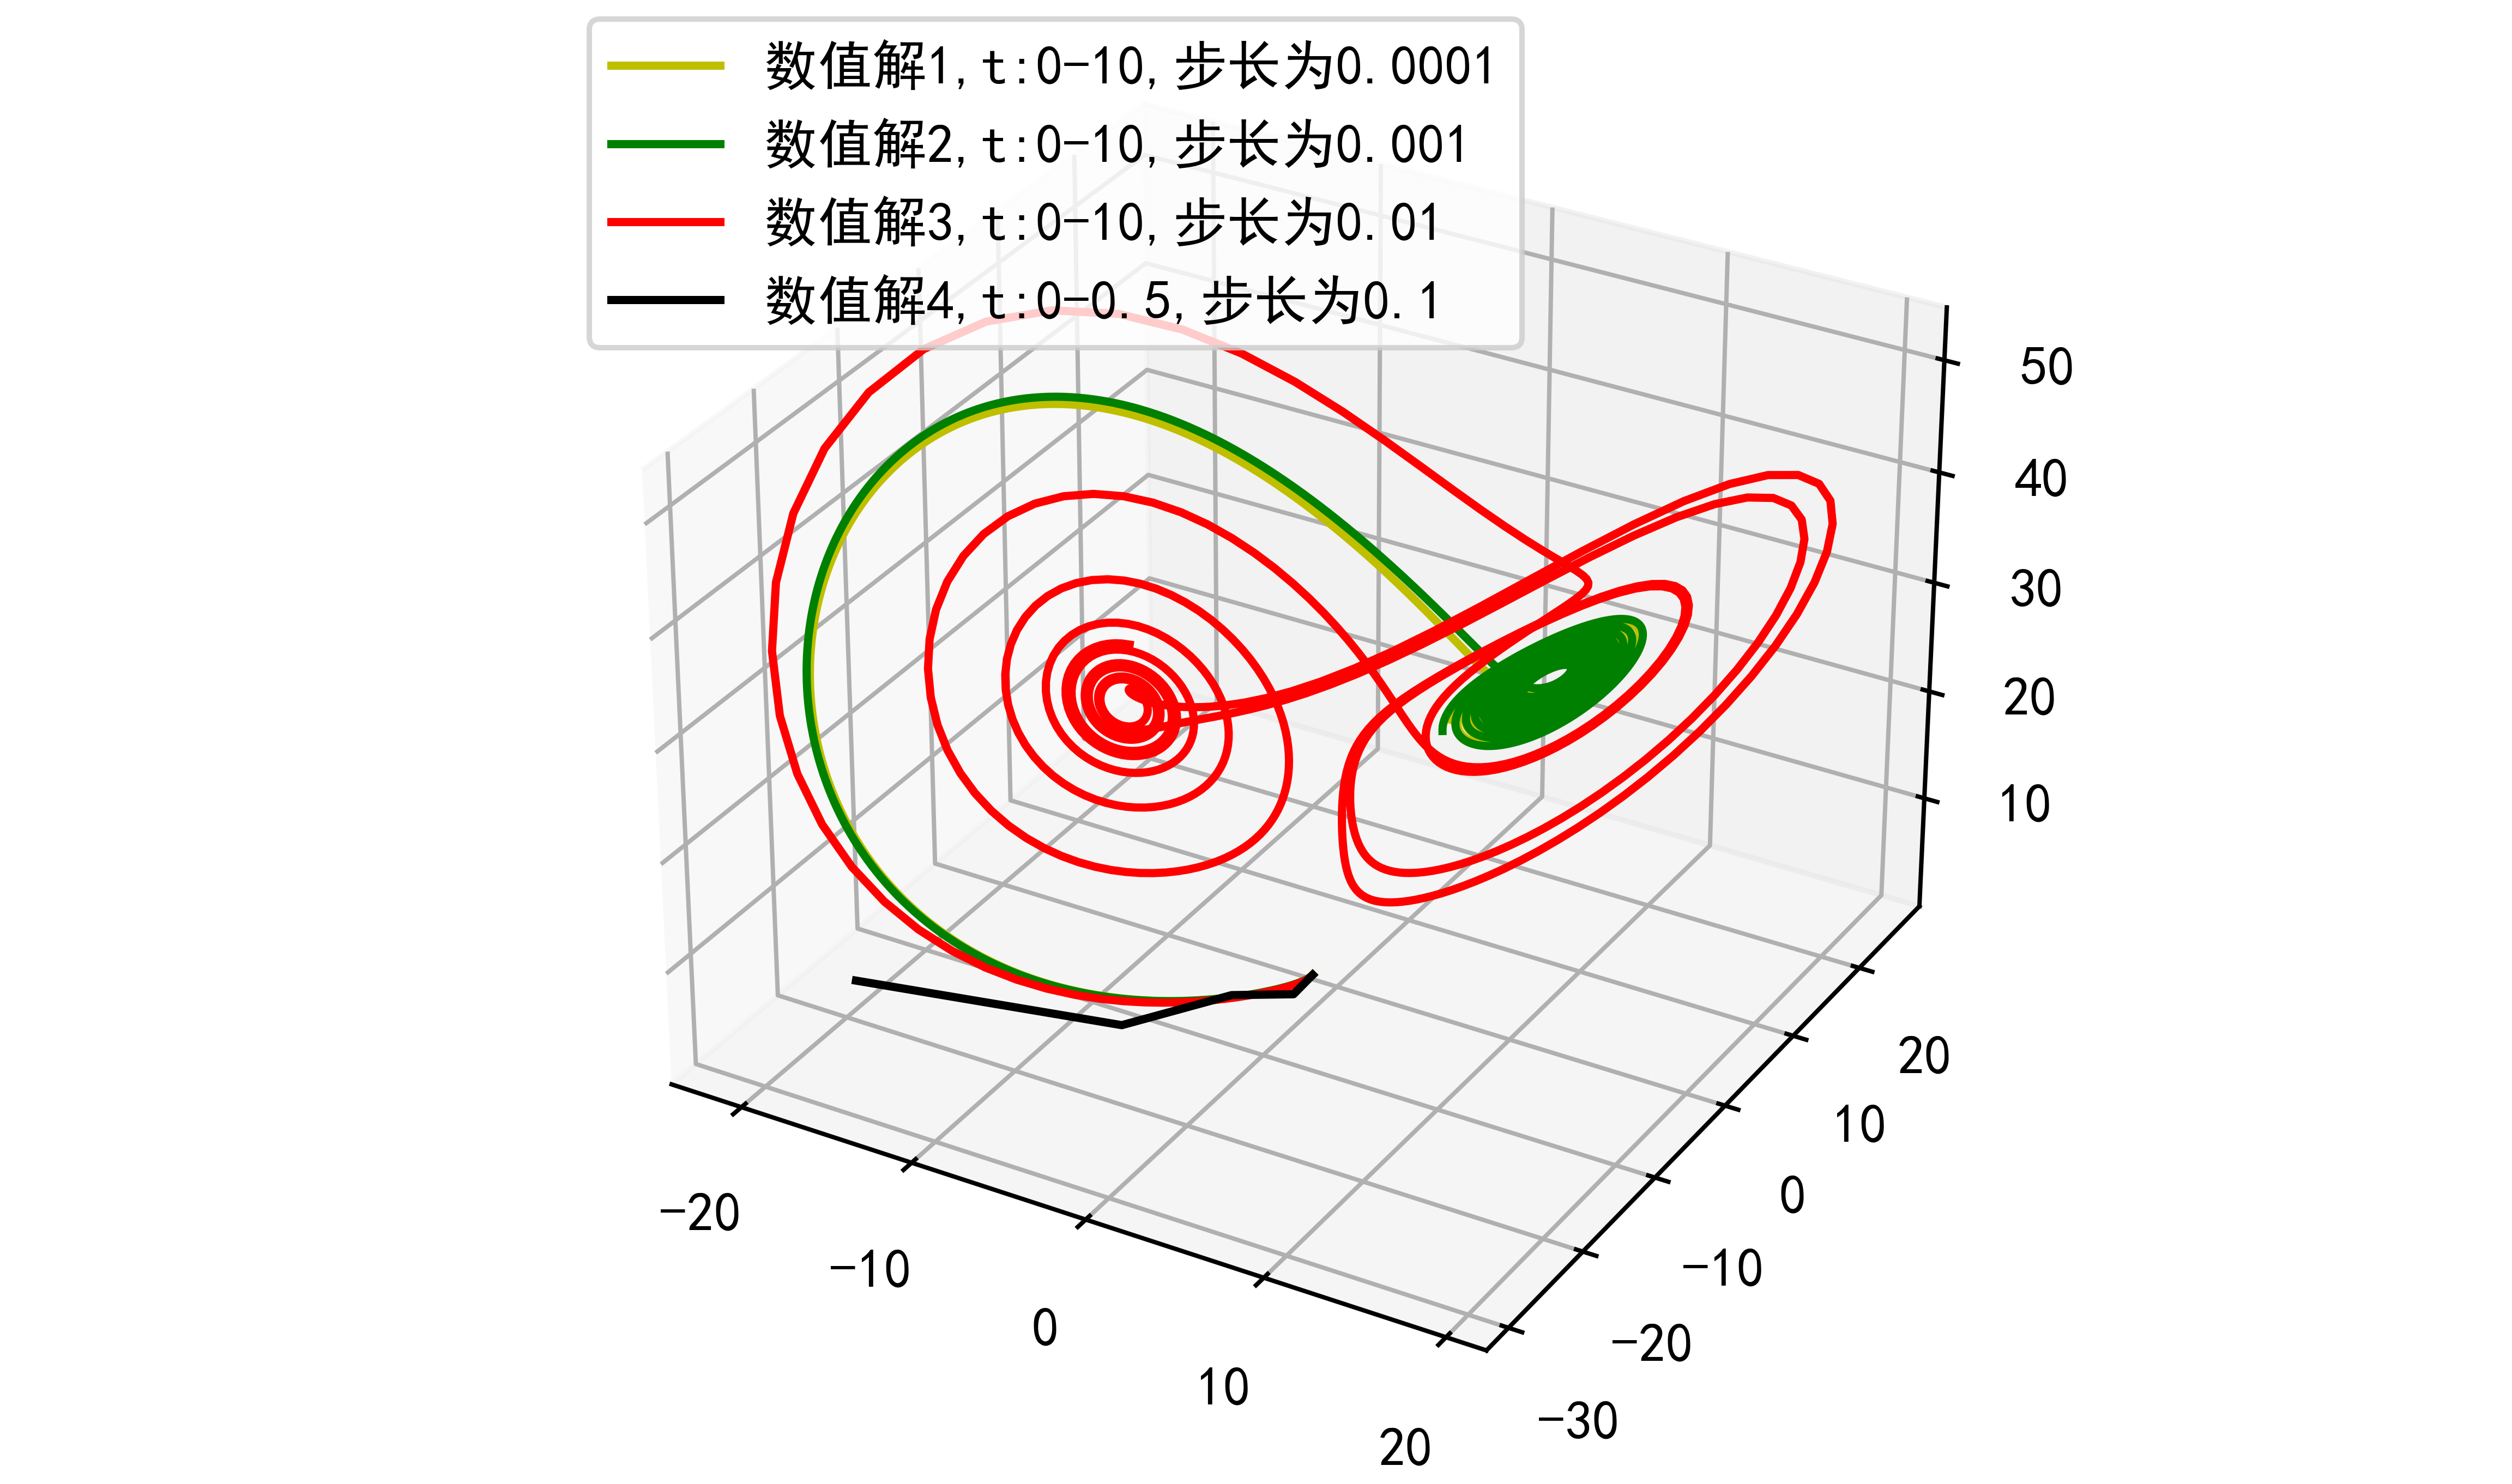
\includegraphics[scale=0.8]{55}
    \caption{起始点为(-1,-1,1)}
\end{figure}

\begin{figure}[h]
    \begin{minipage}{0.48\linewidth}
    \centering
    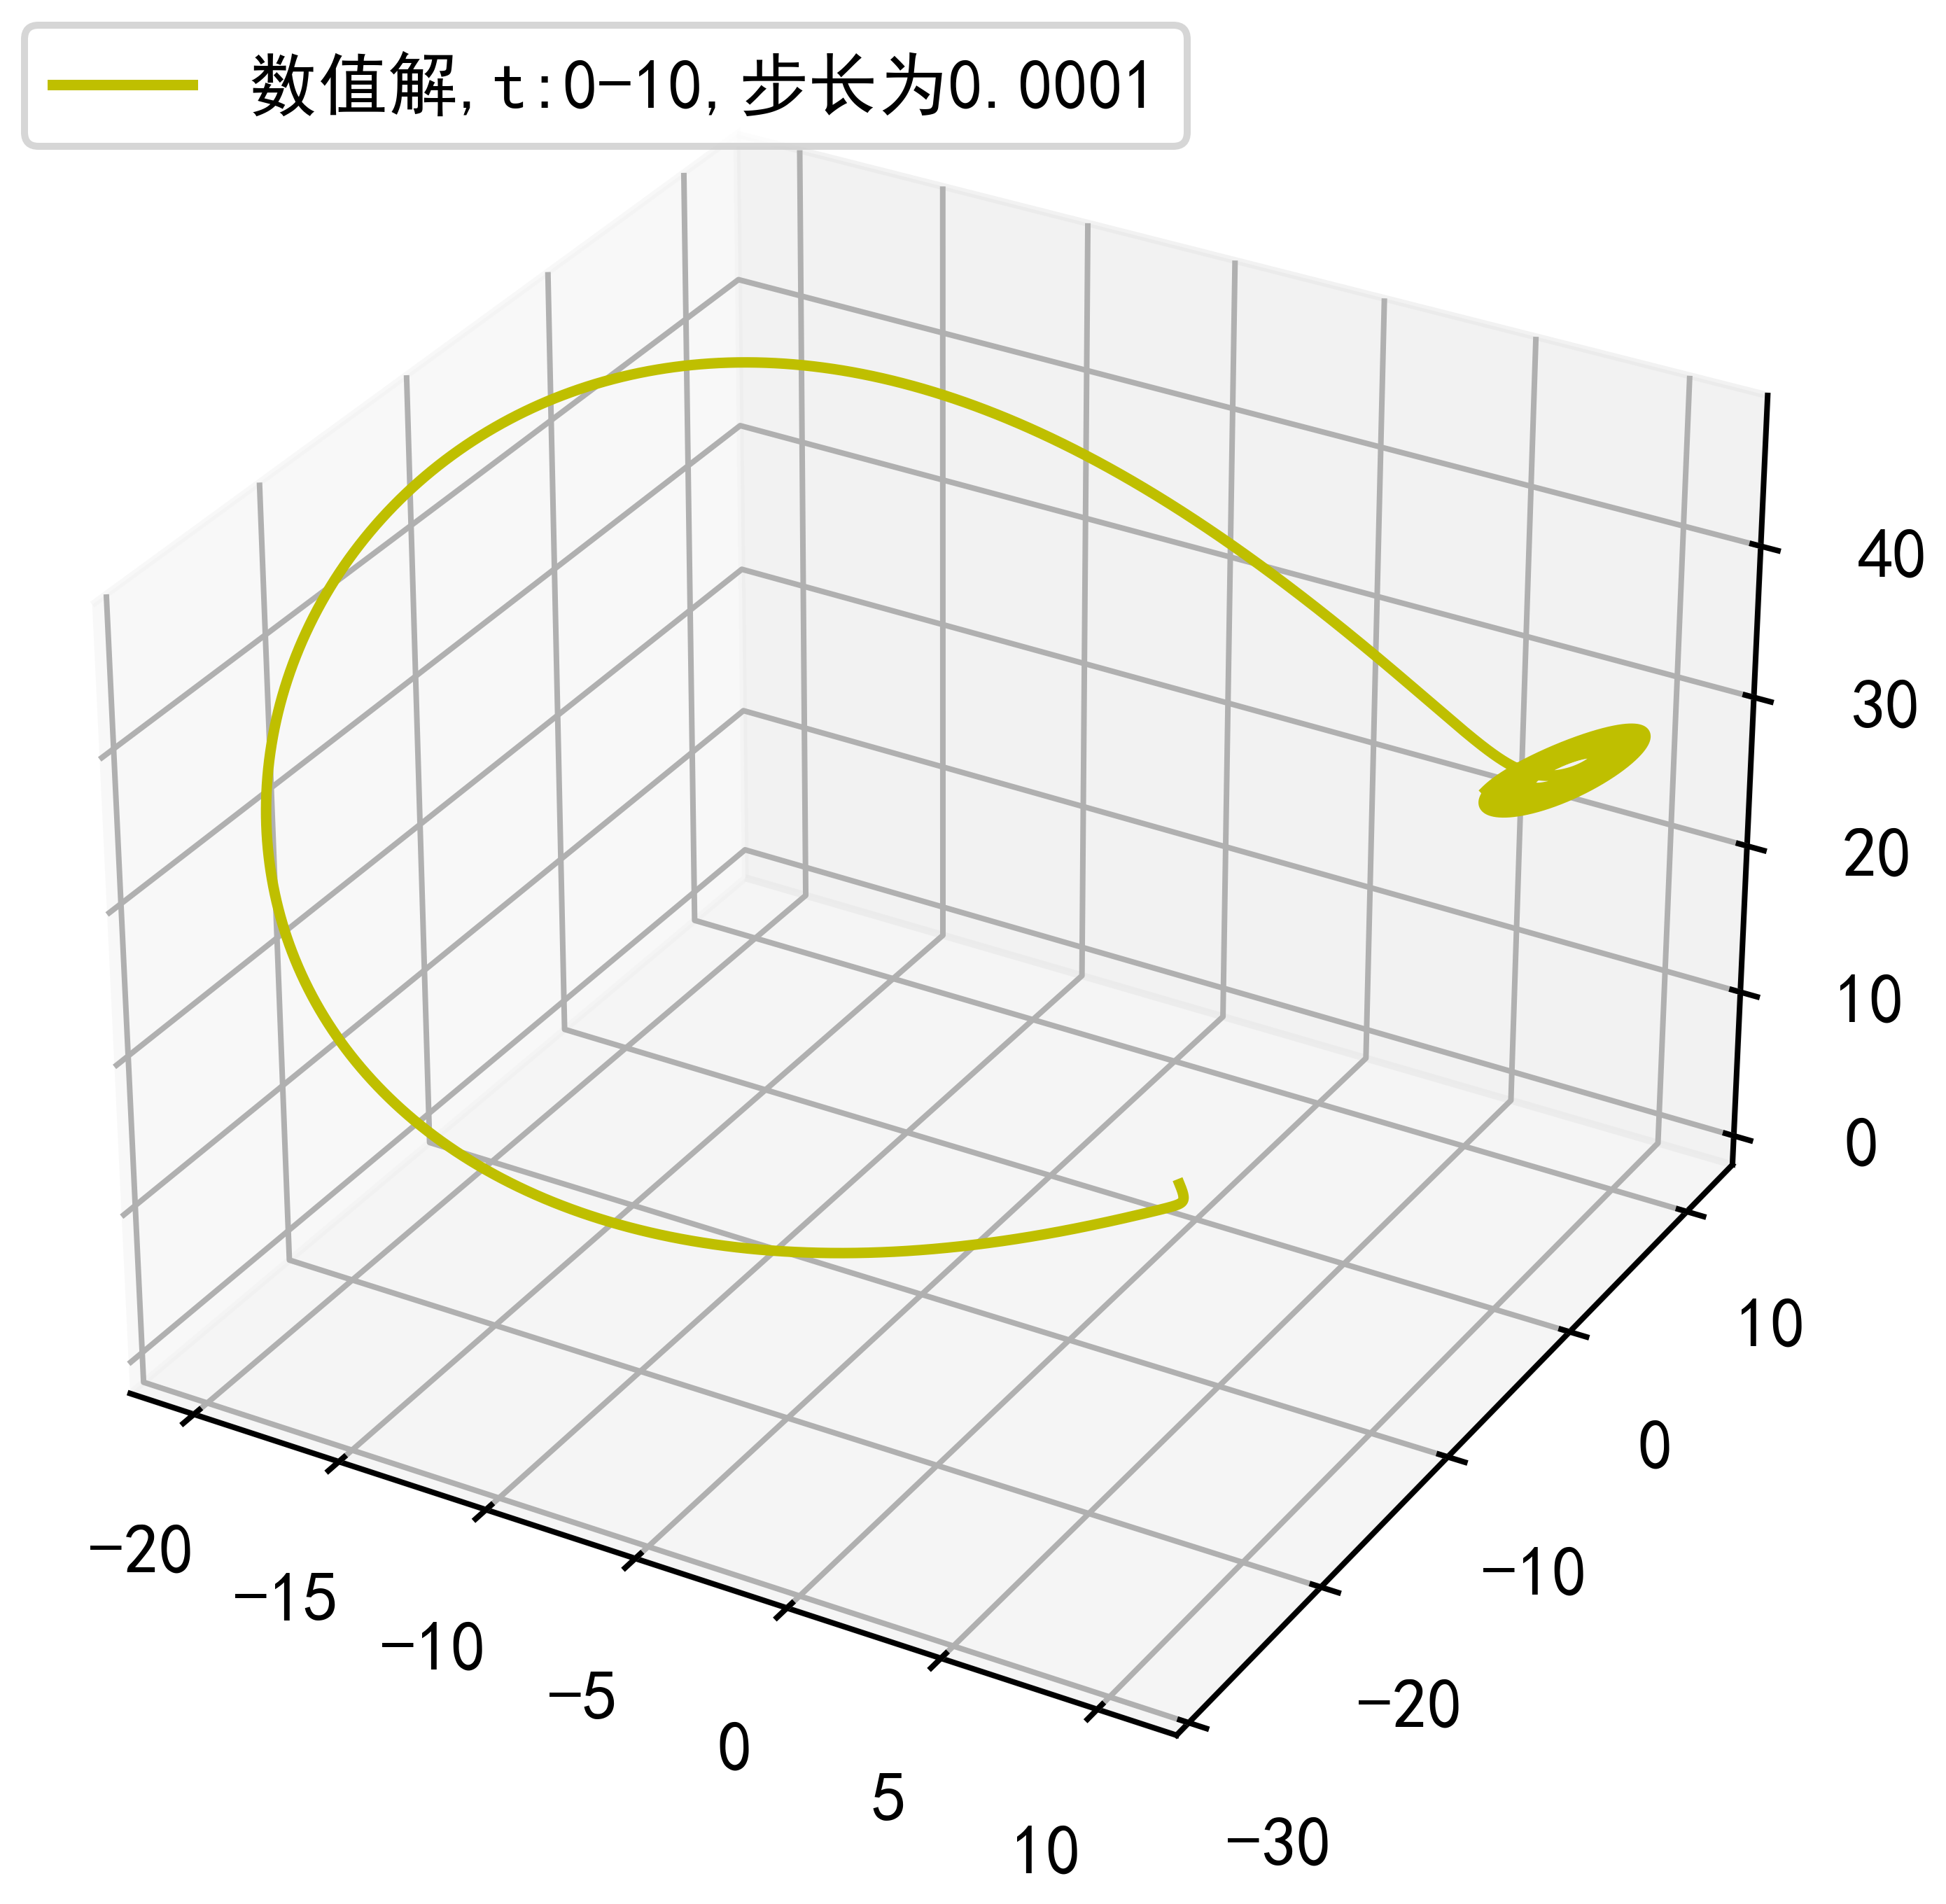
\includegraphics[scale=0.65]{61}
    \caption{起始点为(-1,1,-1)}
    \end{minipage}
    \begin{minipage}{0.48\linewidth}
    \centering
    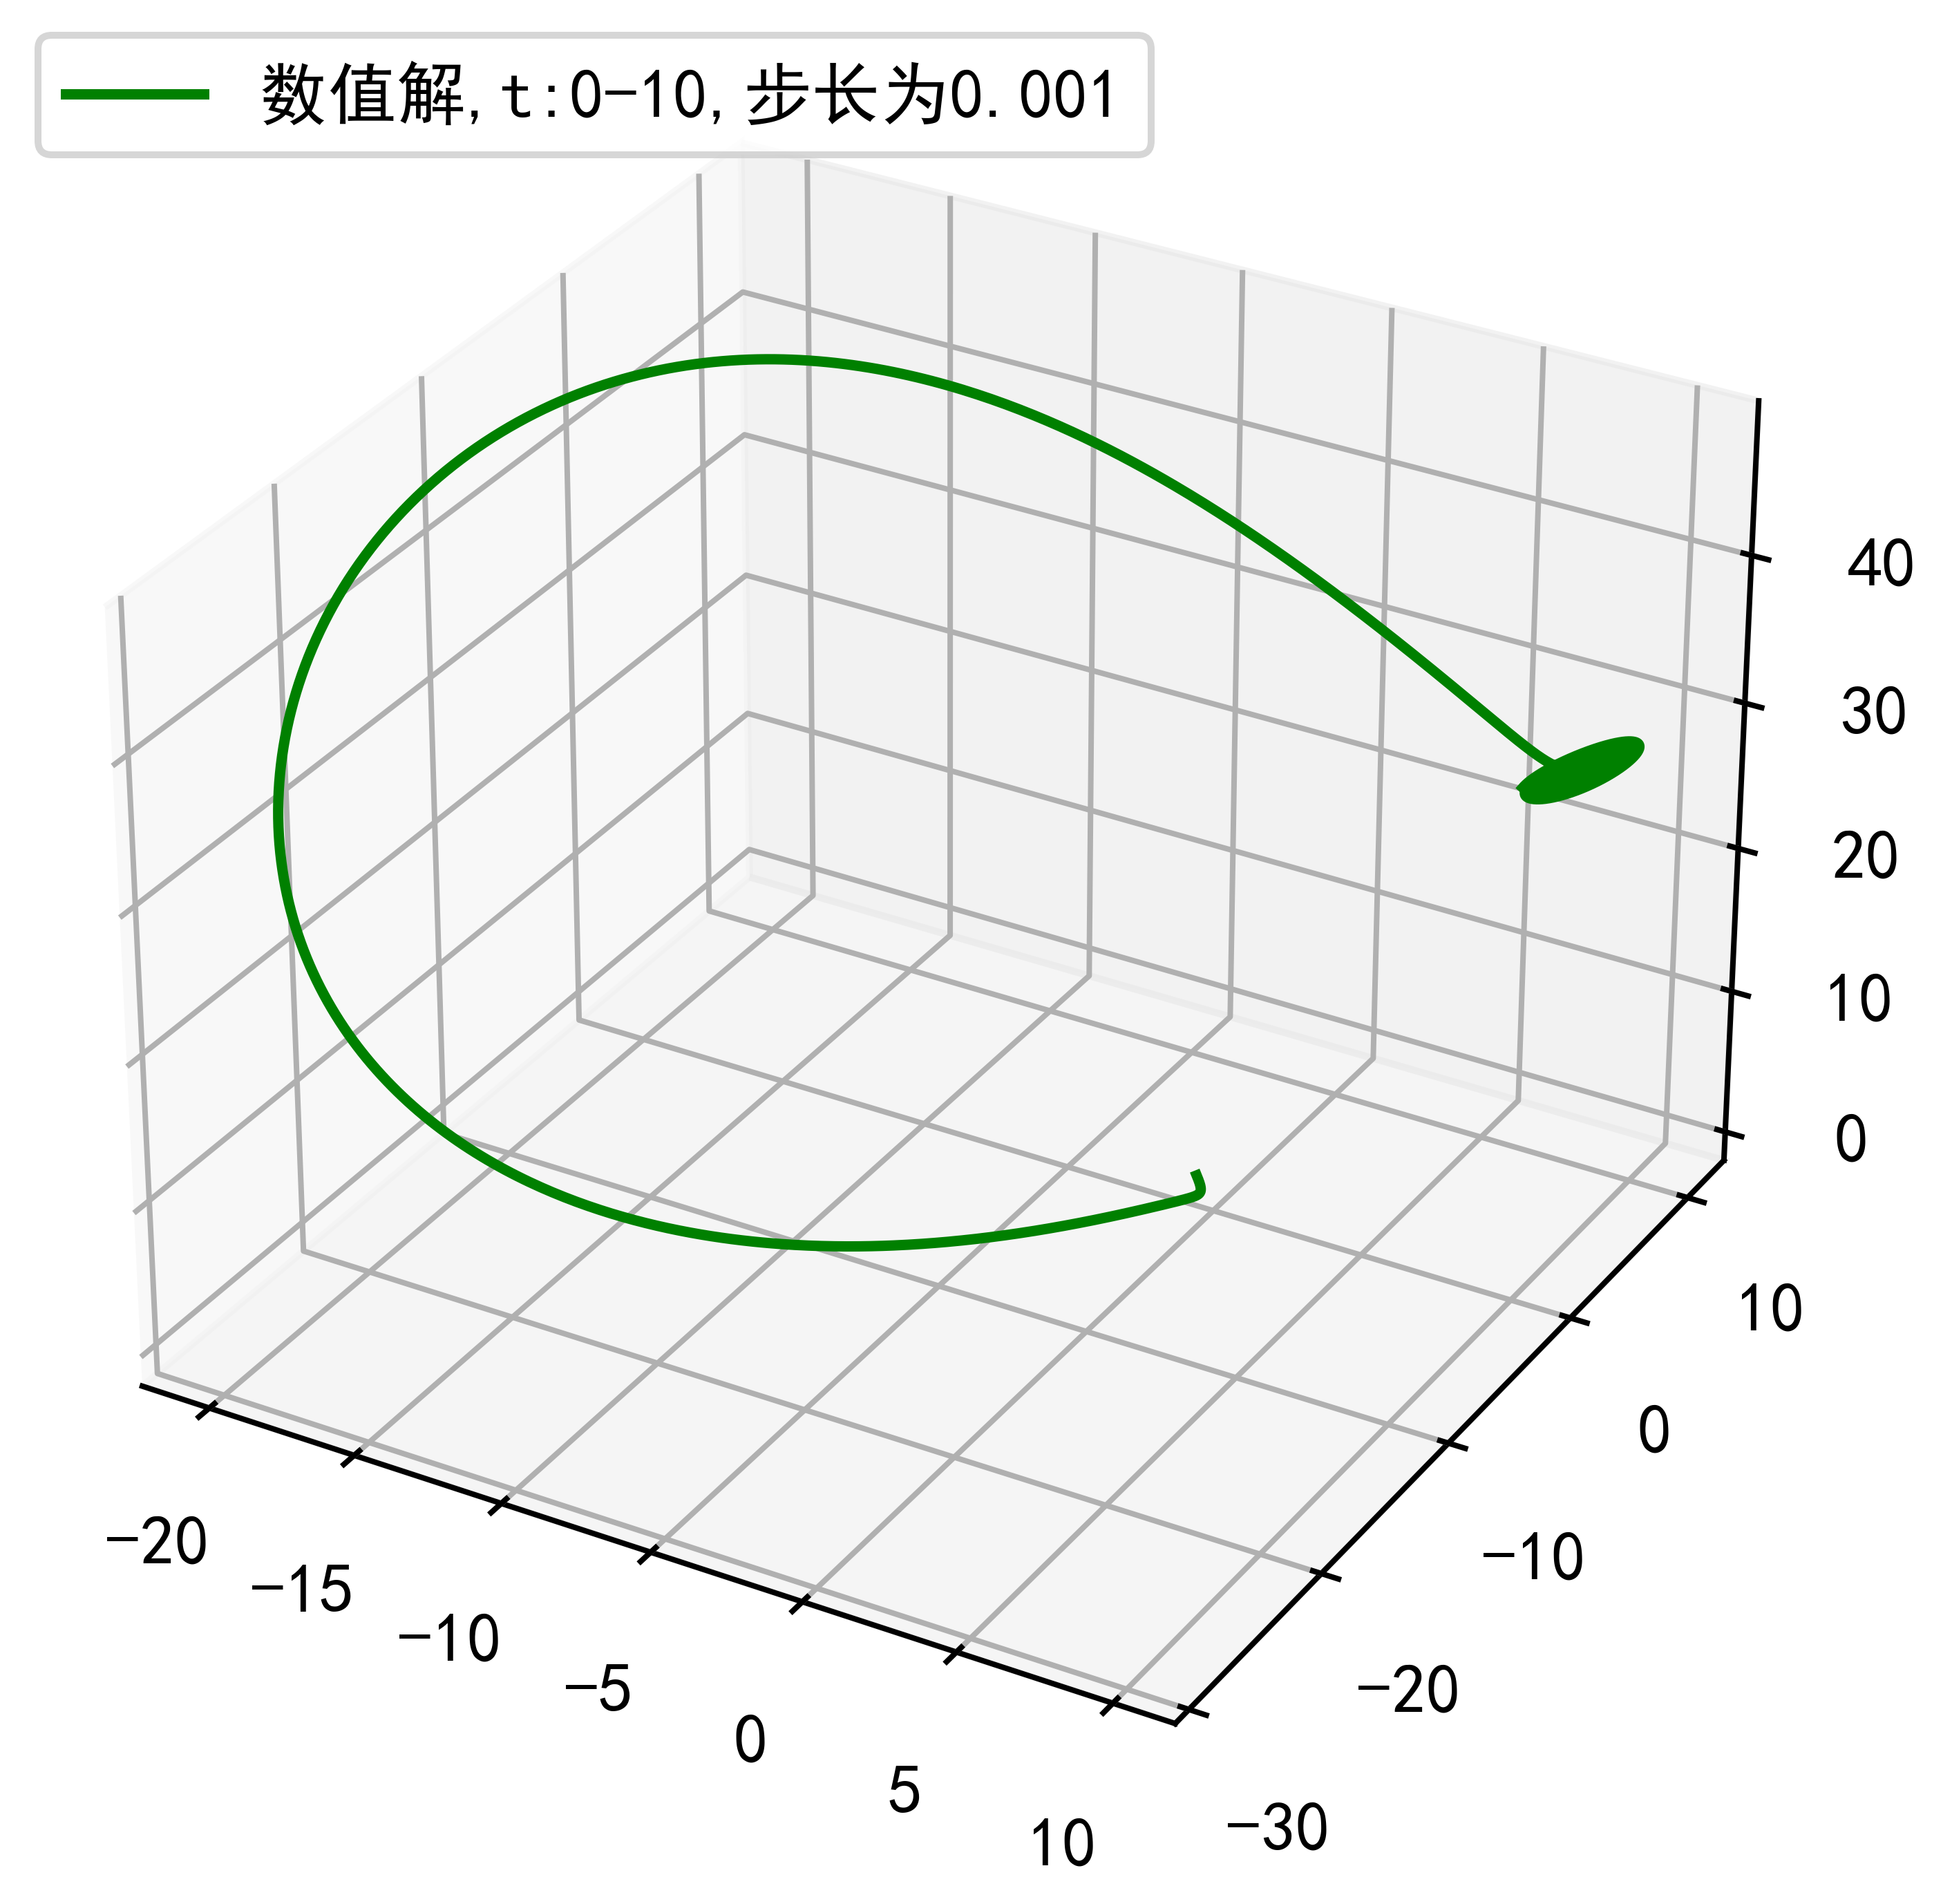
\includegraphics[scale=0.65]{62}
    \caption{起始点为(-1,1,-1)}
    \end{minipage}
\end{figure}
\begin{figure}[h]
    \begin{minipage}[h]{0.48\linewidth}
    \centering
    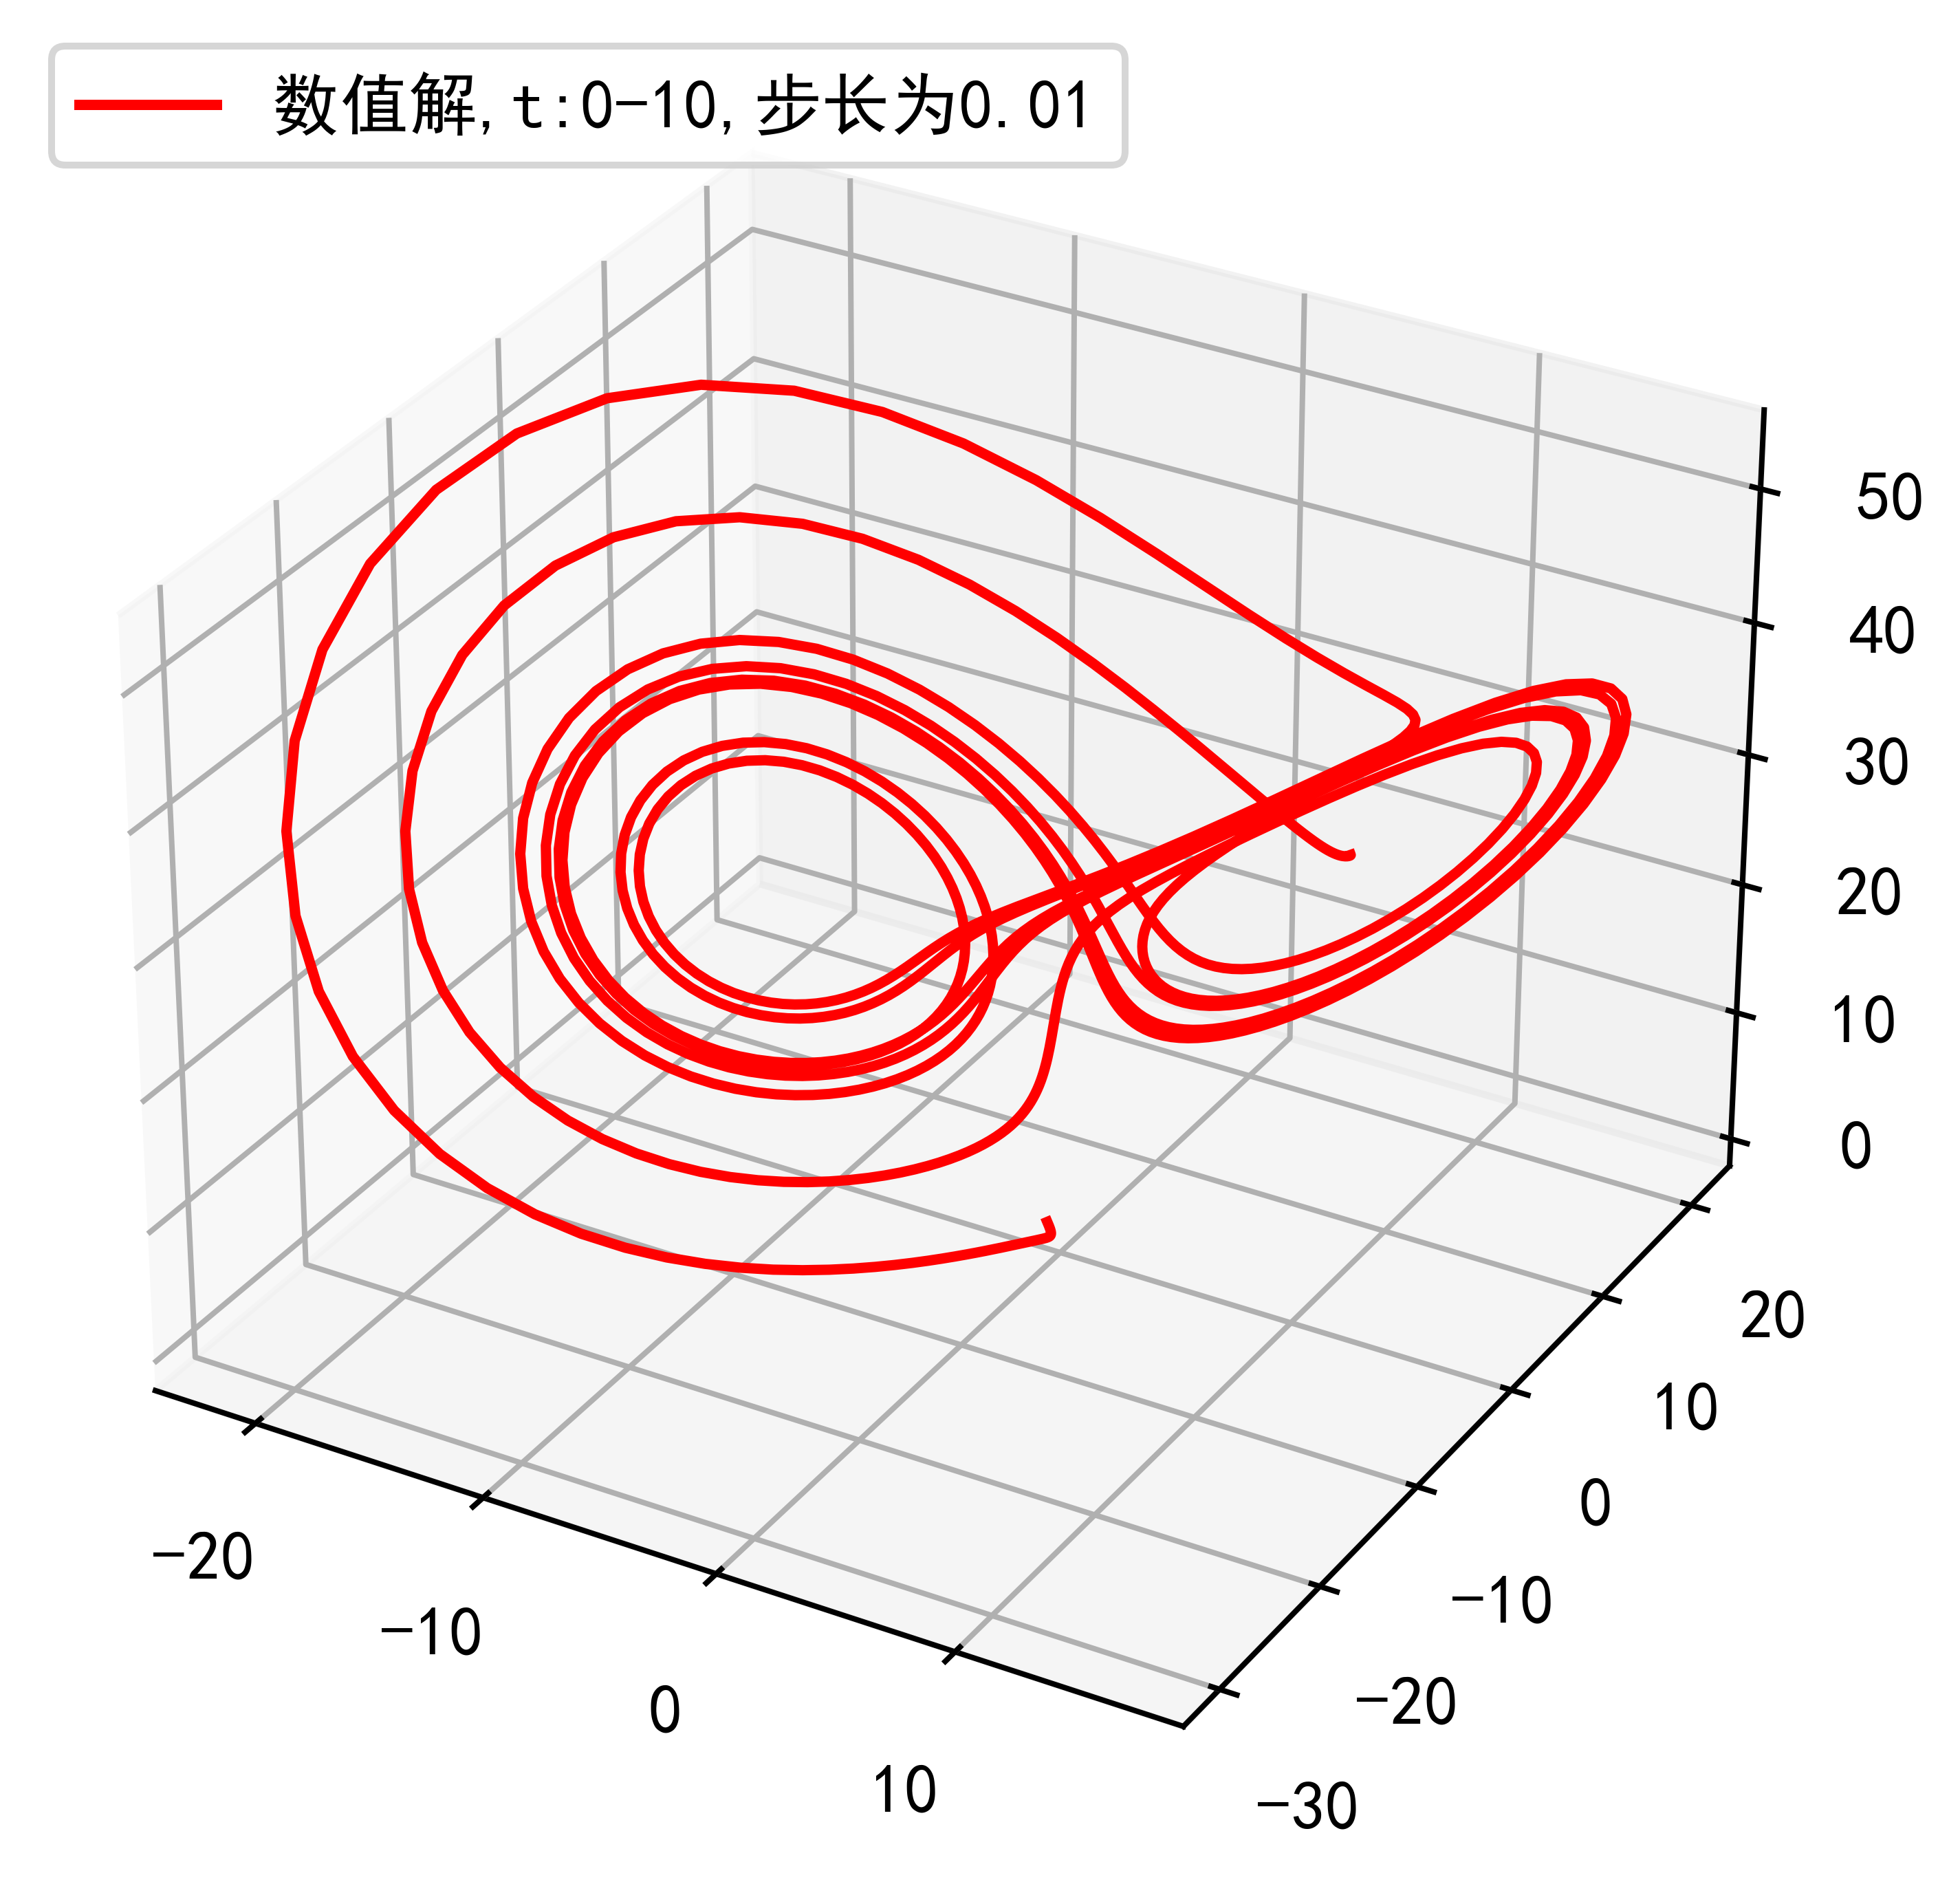
\includegraphics[scale=0.65]{63}
    \caption{起始点为(-1,1,-1)}
    \end{minipage}
    \begin{minipage}[h]{0.48\linewidth}
    \centering
    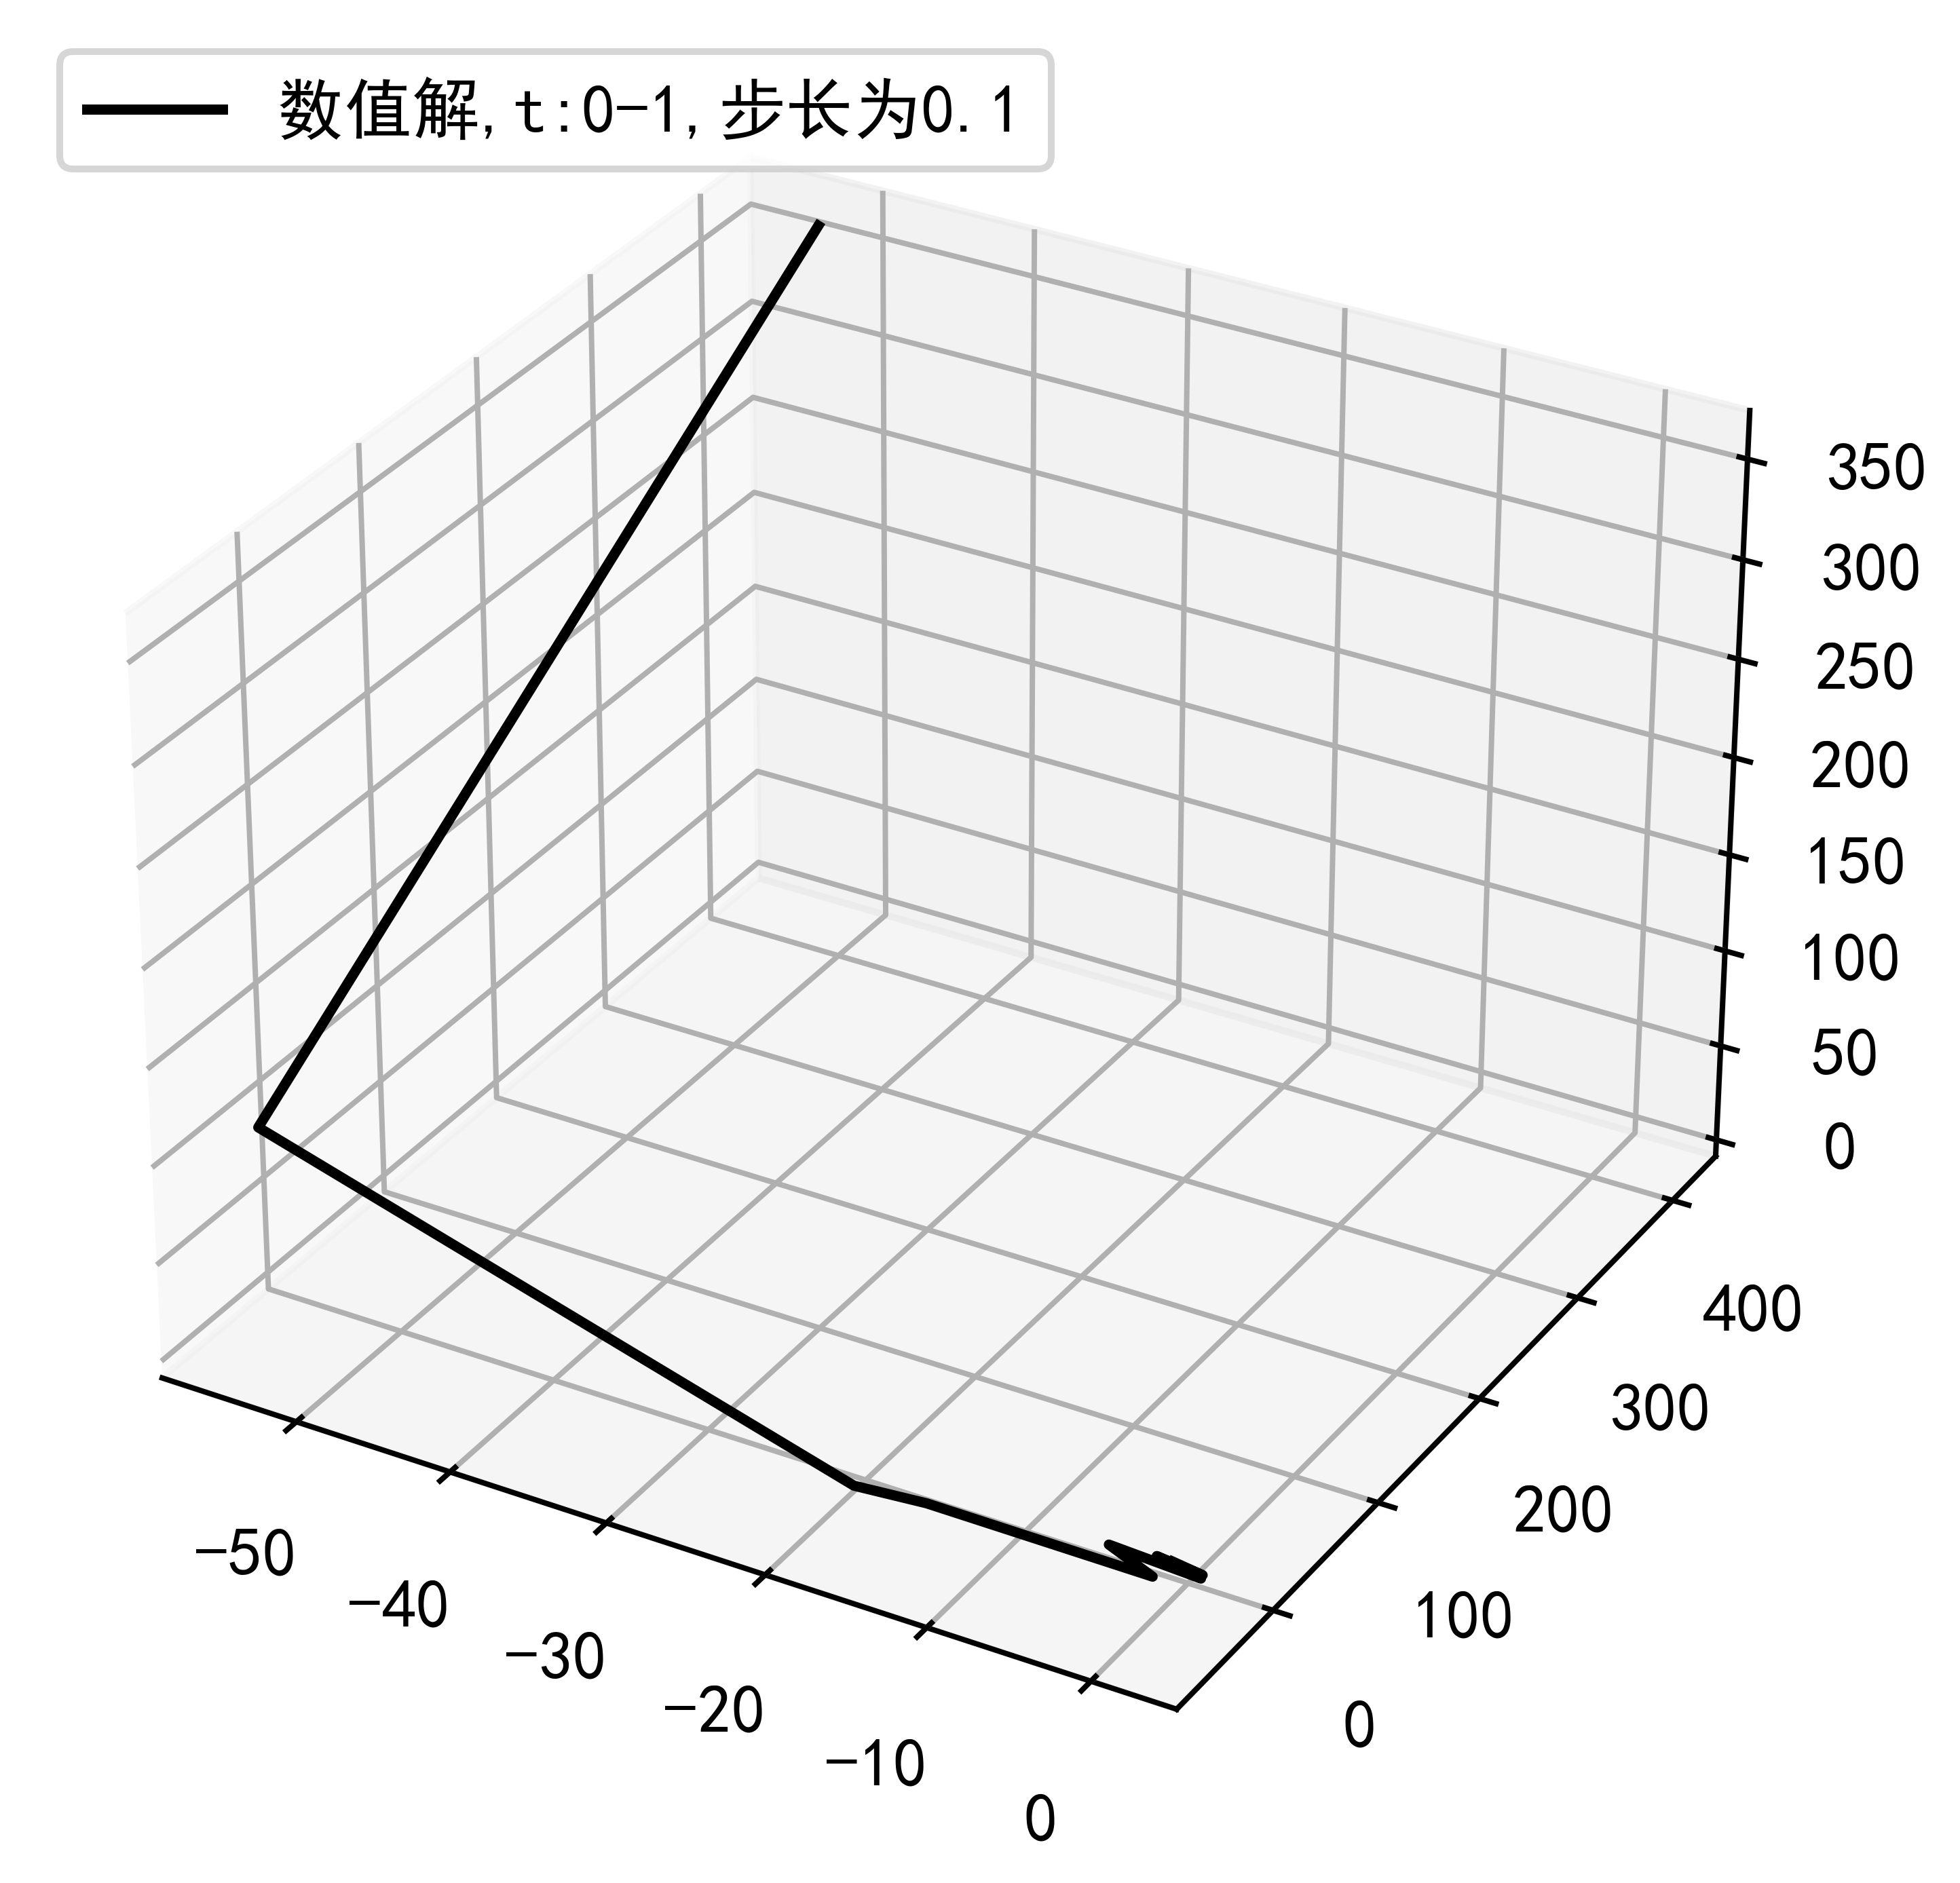
\includegraphics[scale=0.65]{64}
    \caption{起始点为(-1,1,-1)}
    \end{minipage}
\end{figure}
\begin{figure}[H]
    \centering
    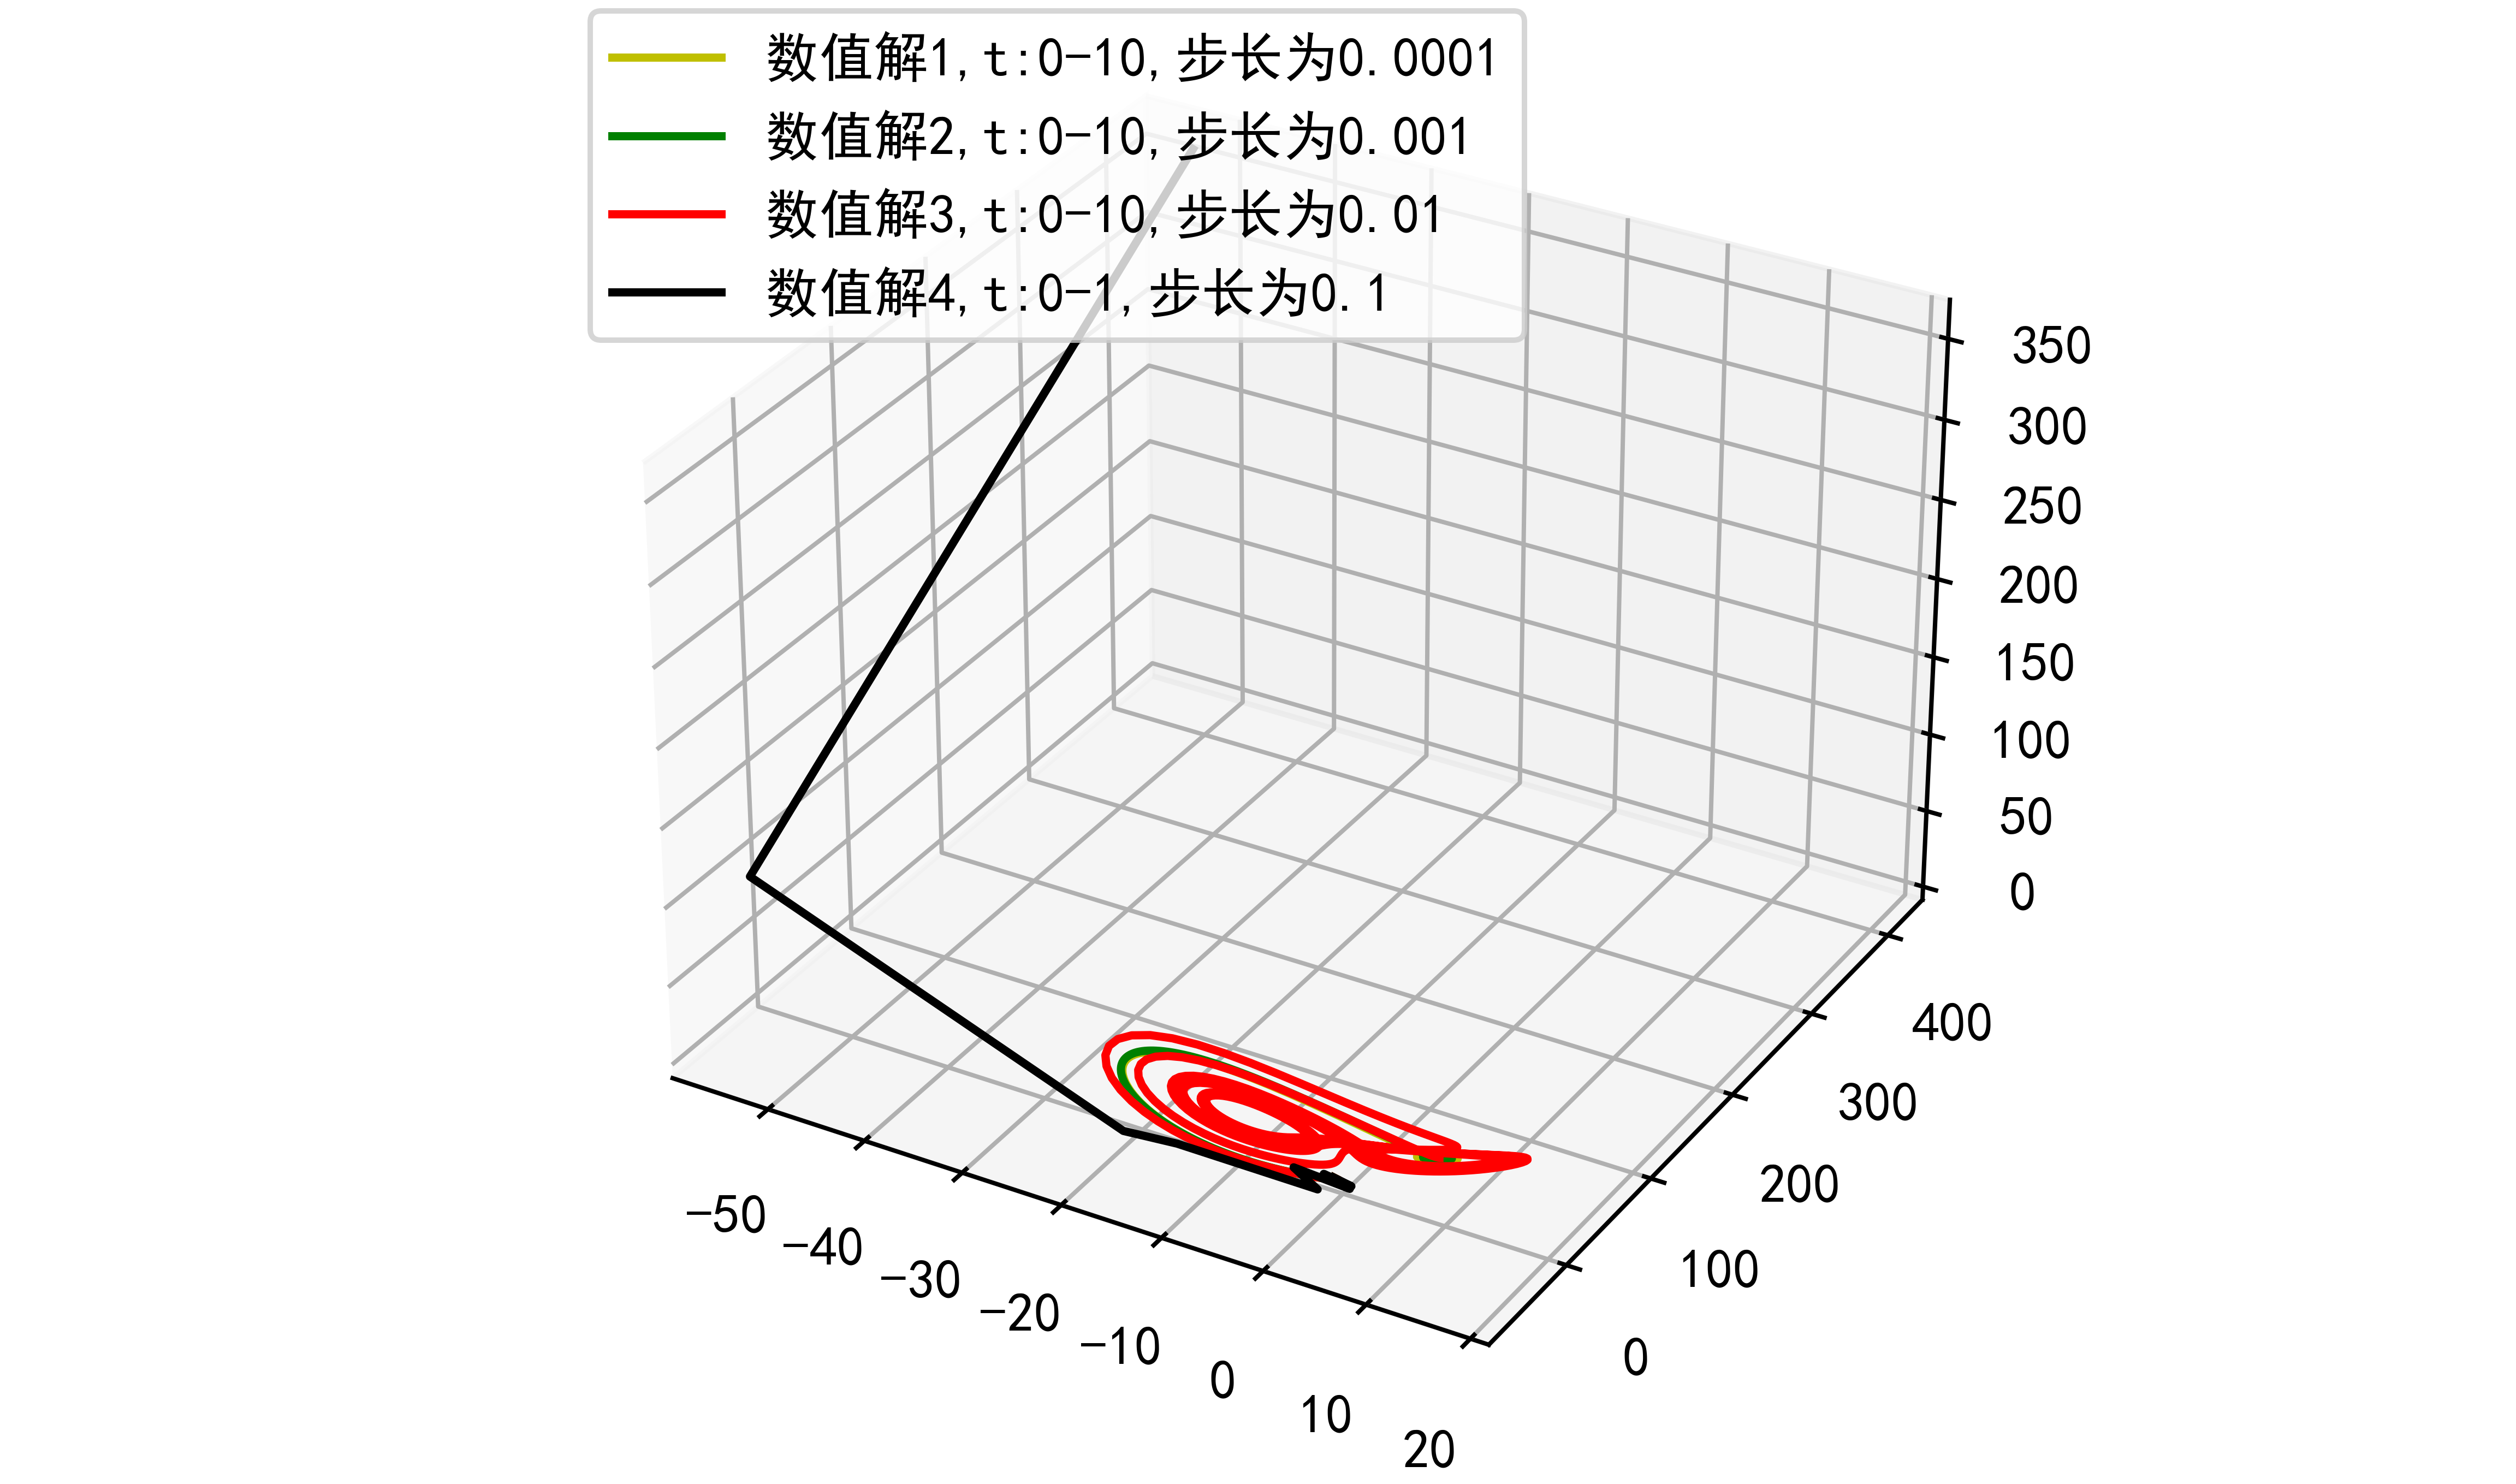
\includegraphics[scale=0.8]{65}
    \caption{起始点为(-1,1,-1)}
\end{figure}

\begin{figure}[h]
    \begin{minipage}{0.48\linewidth}
    \centering
    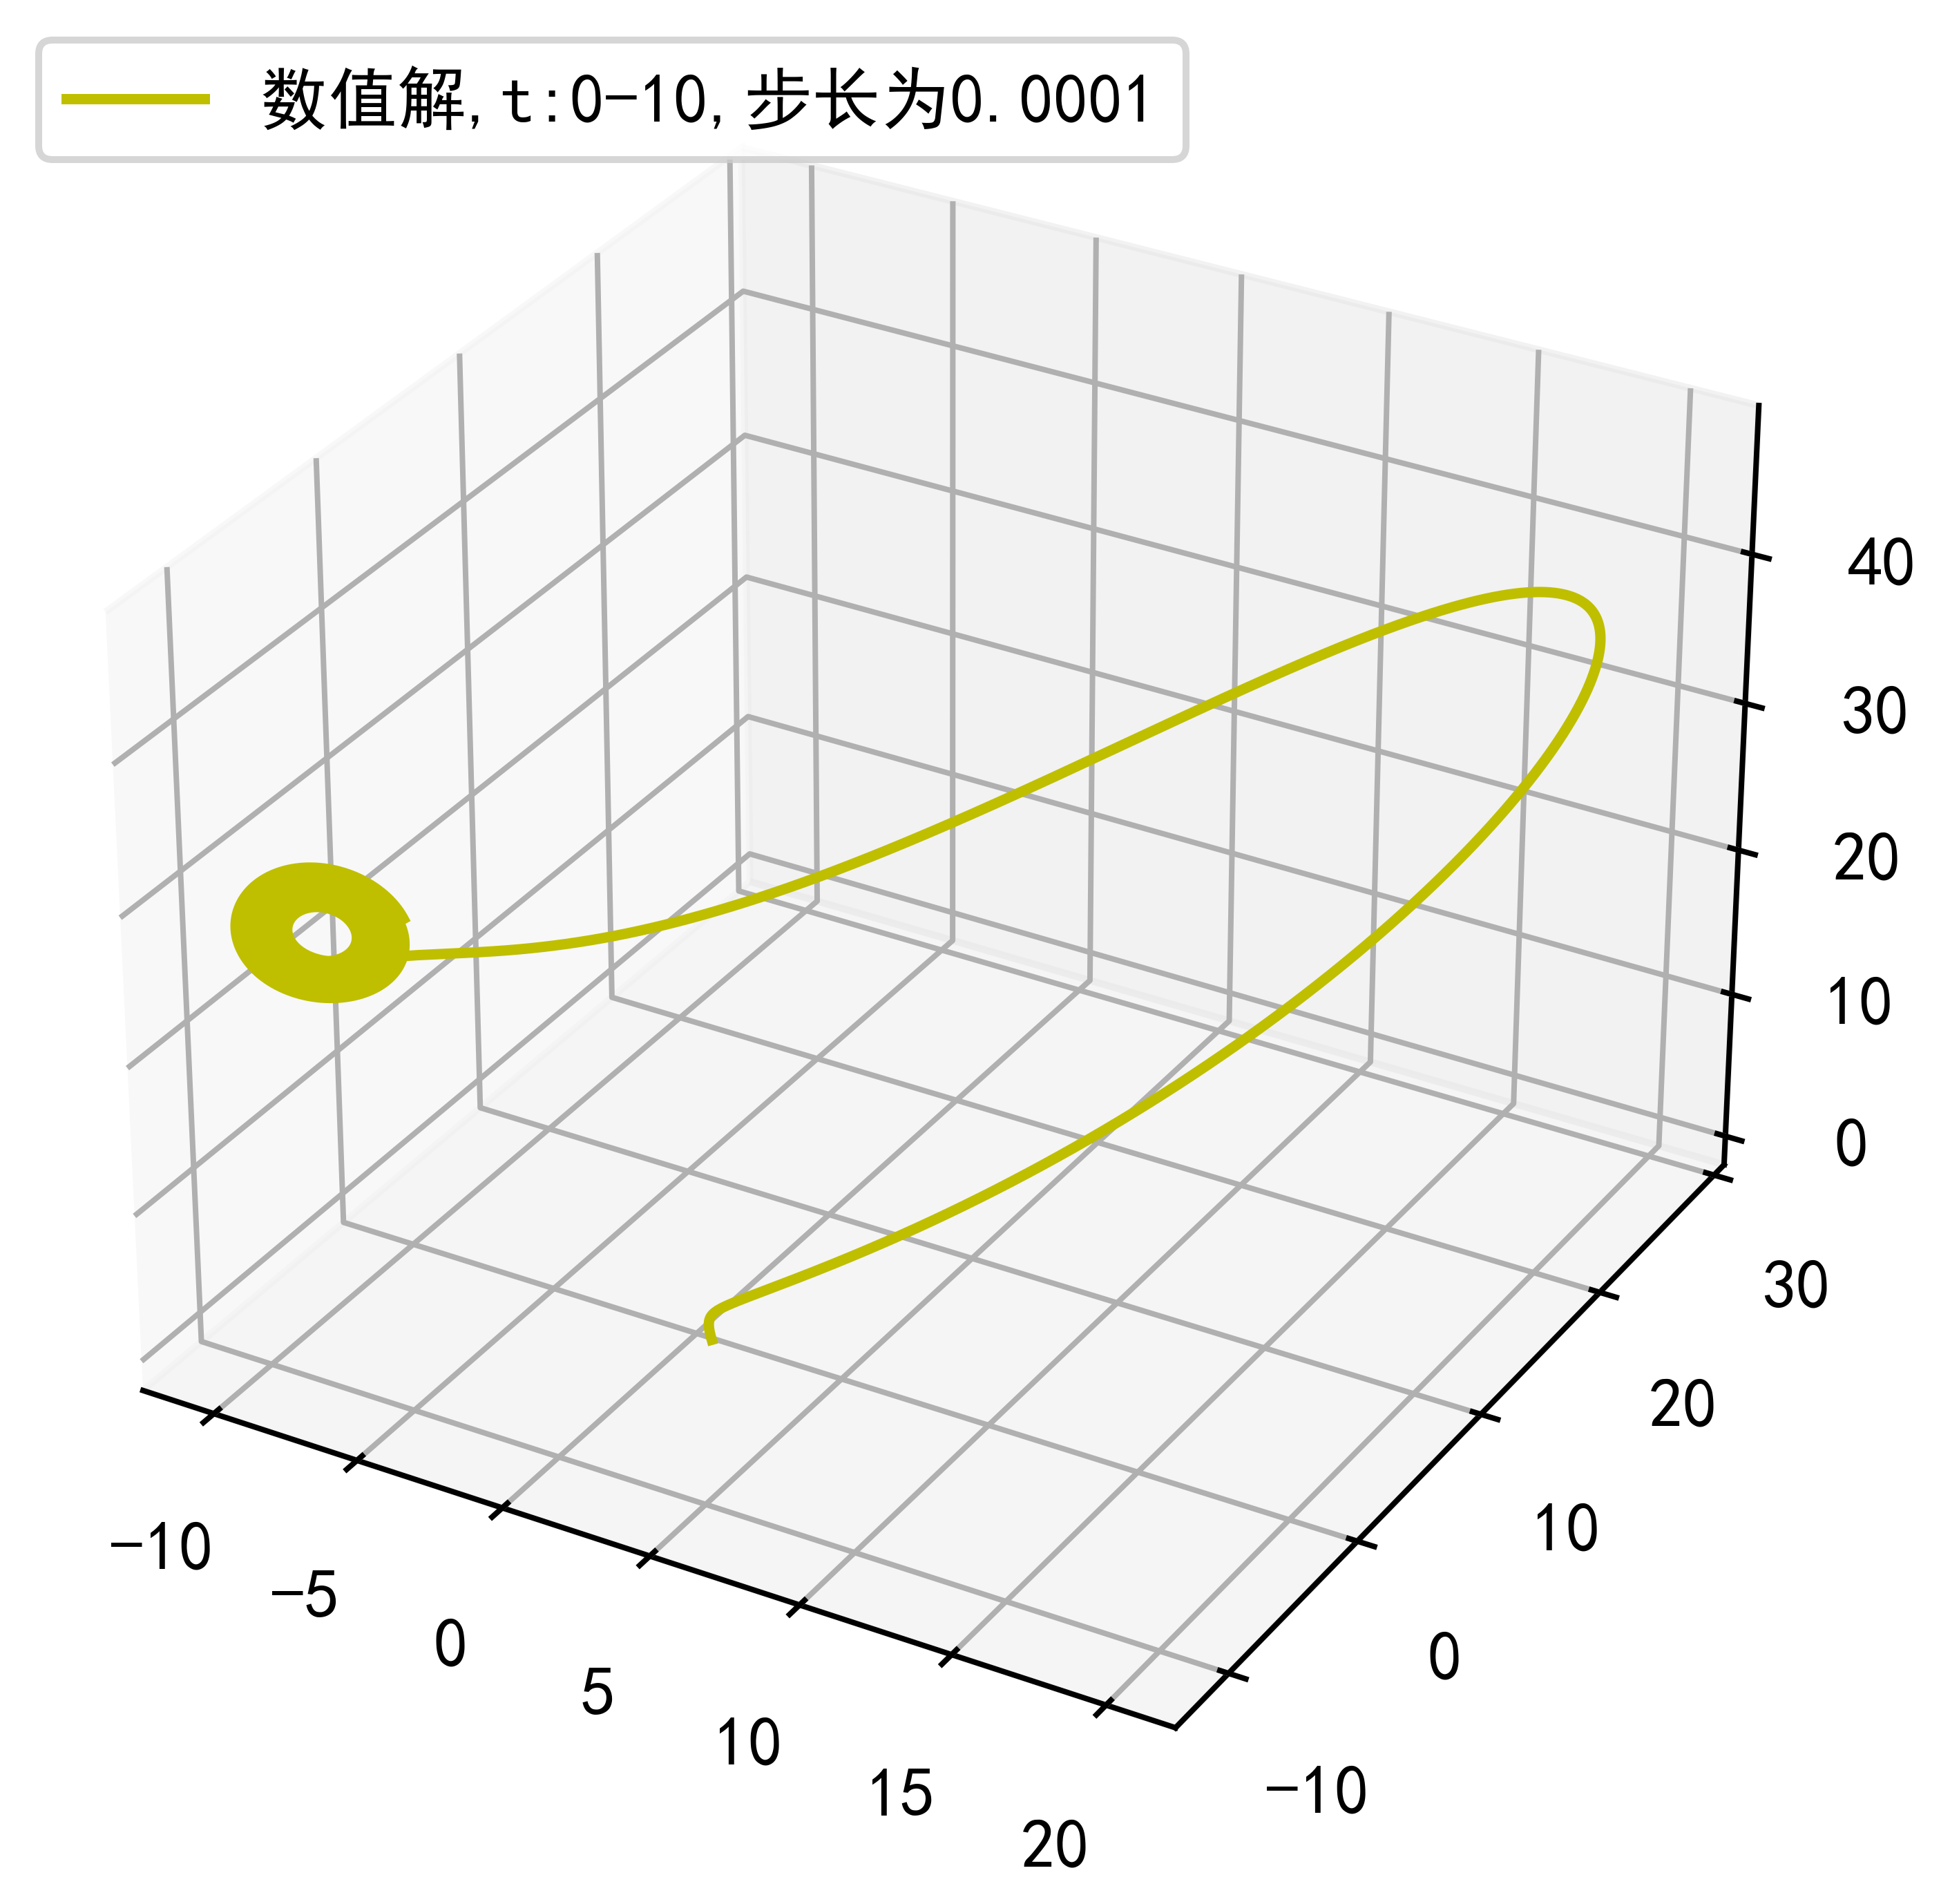
\includegraphics[scale=0.65]{71}
    \caption{起始点为(1,-1,-1)}
    \end{minipage}
    \begin{minipage}{0.48\linewidth}
    \centering
    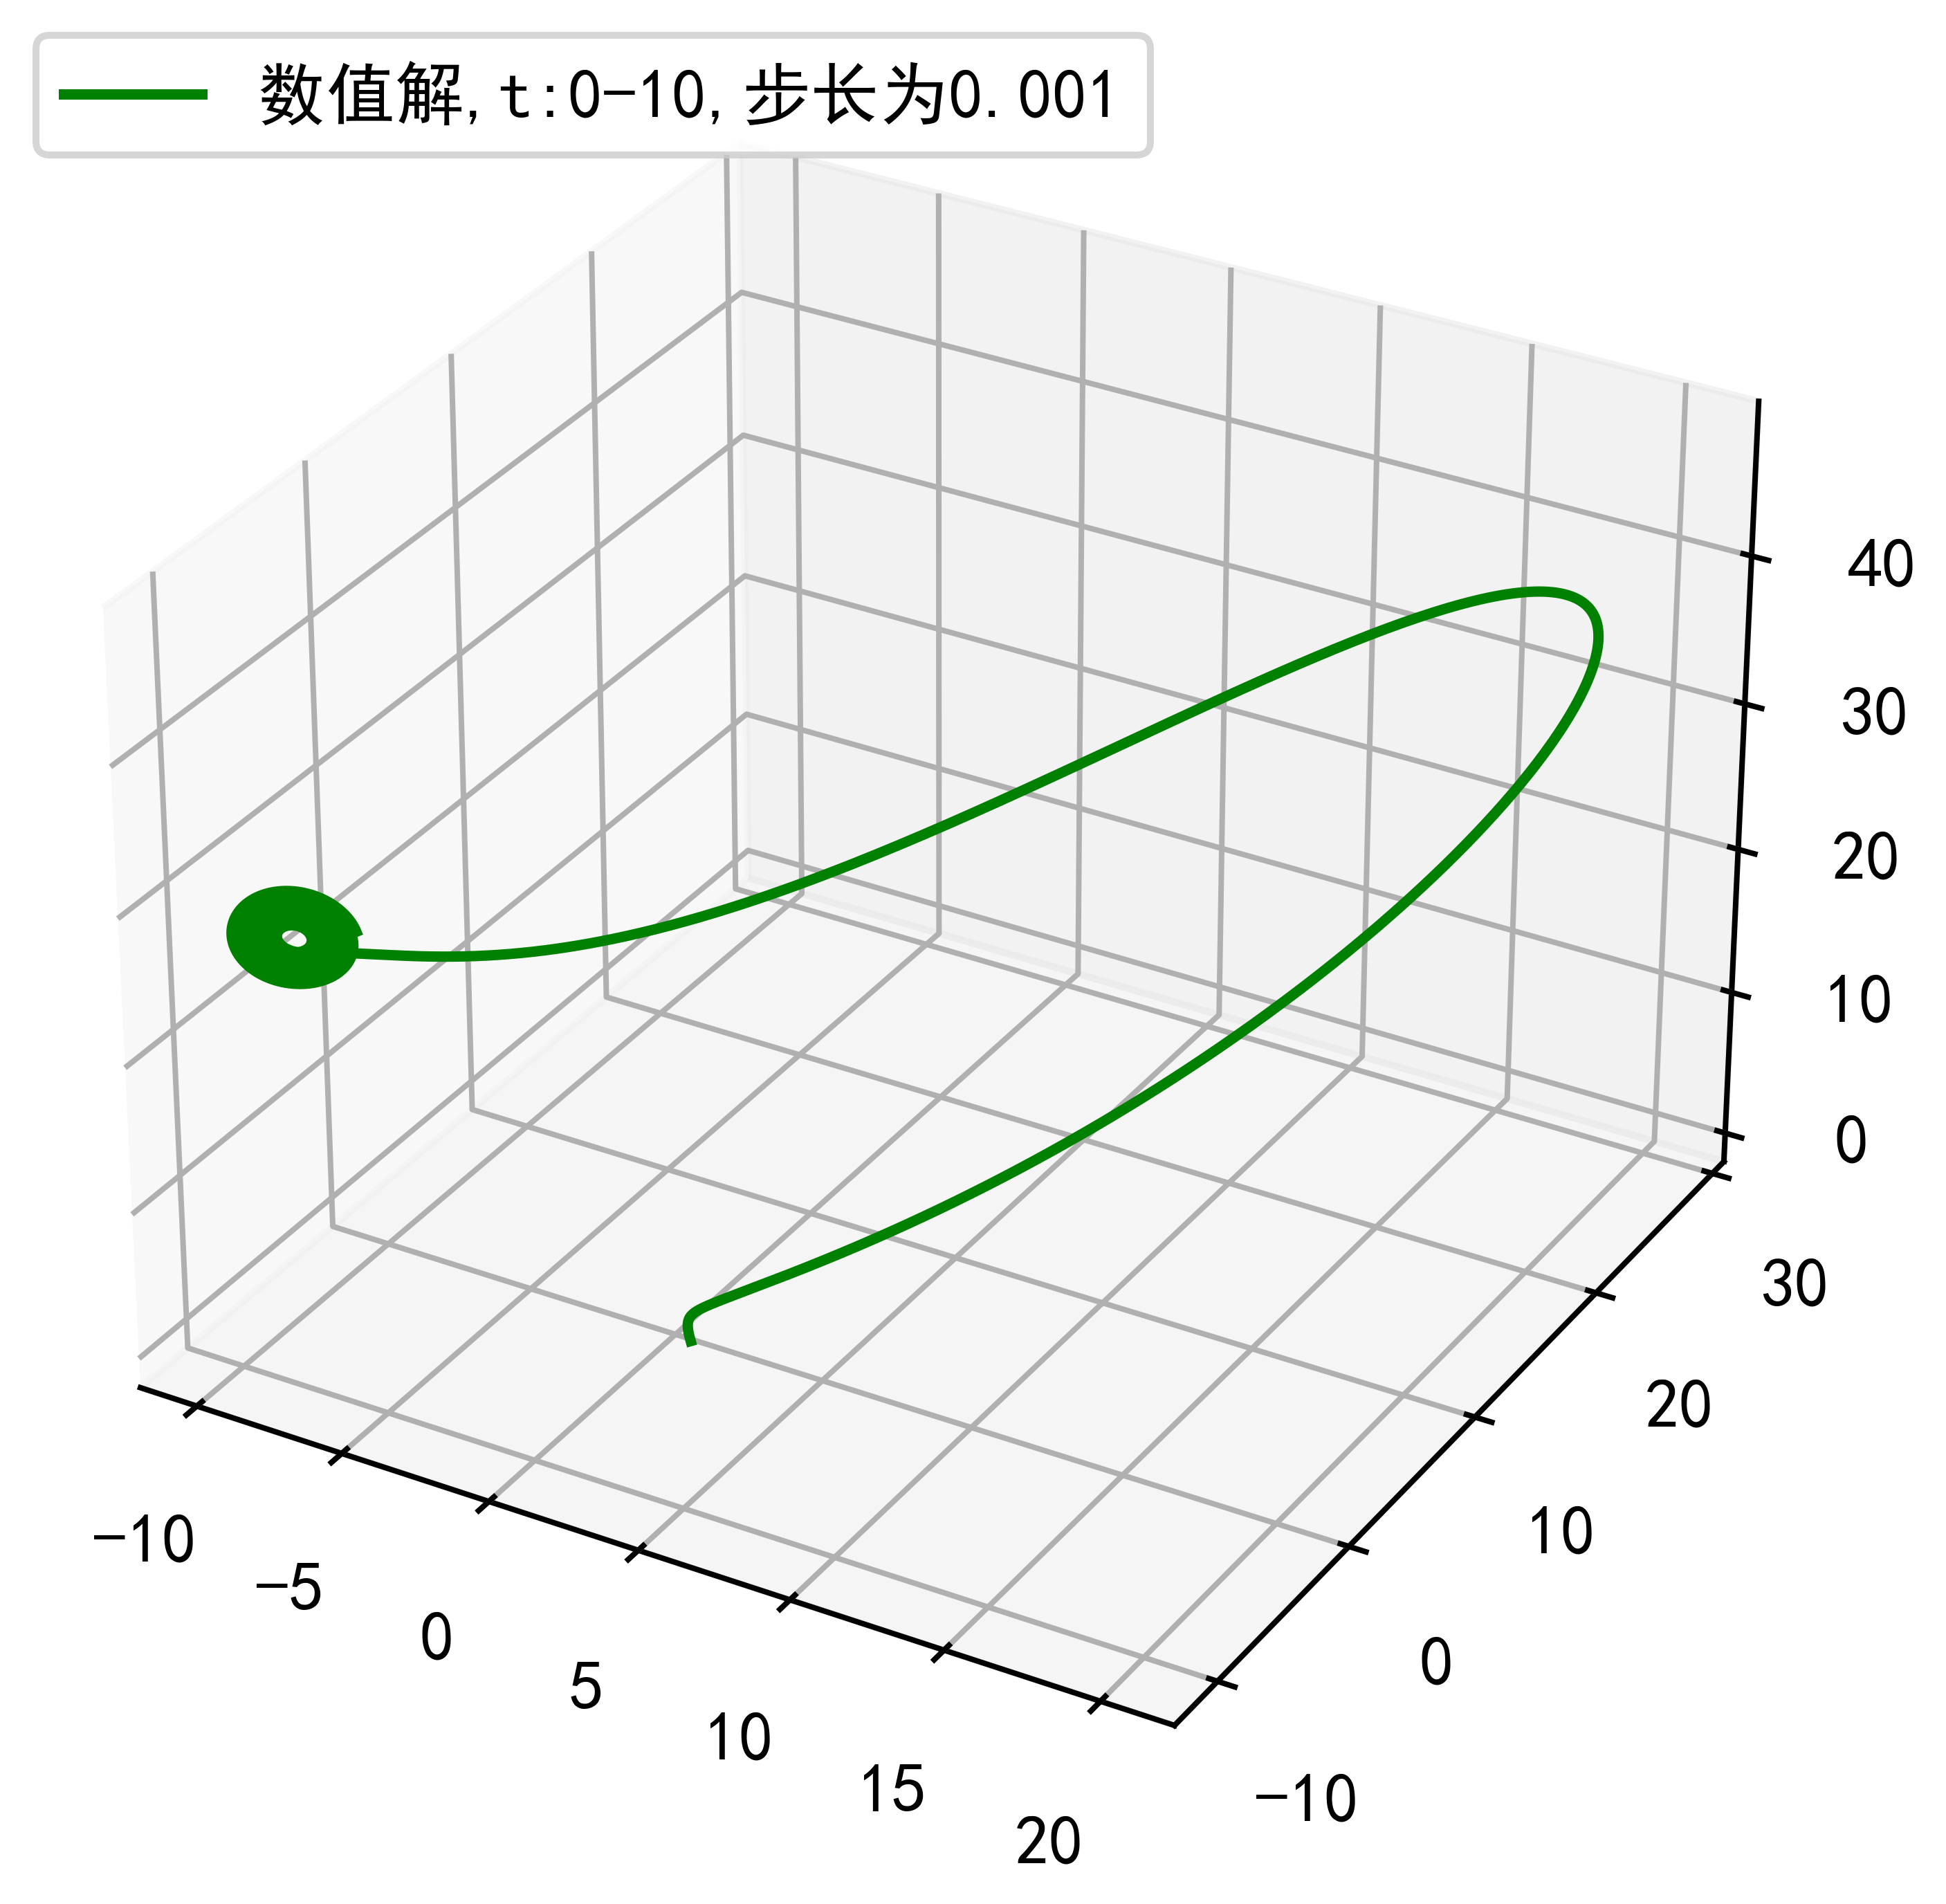
\includegraphics[scale=0.65]{72}
    \caption{起始点为(1,-1,-1)}
    \end{minipage}
\end{figure}
\begin{figure}[h]
    \begin{minipage}[h]{0.48\linewidth}
    \centering
    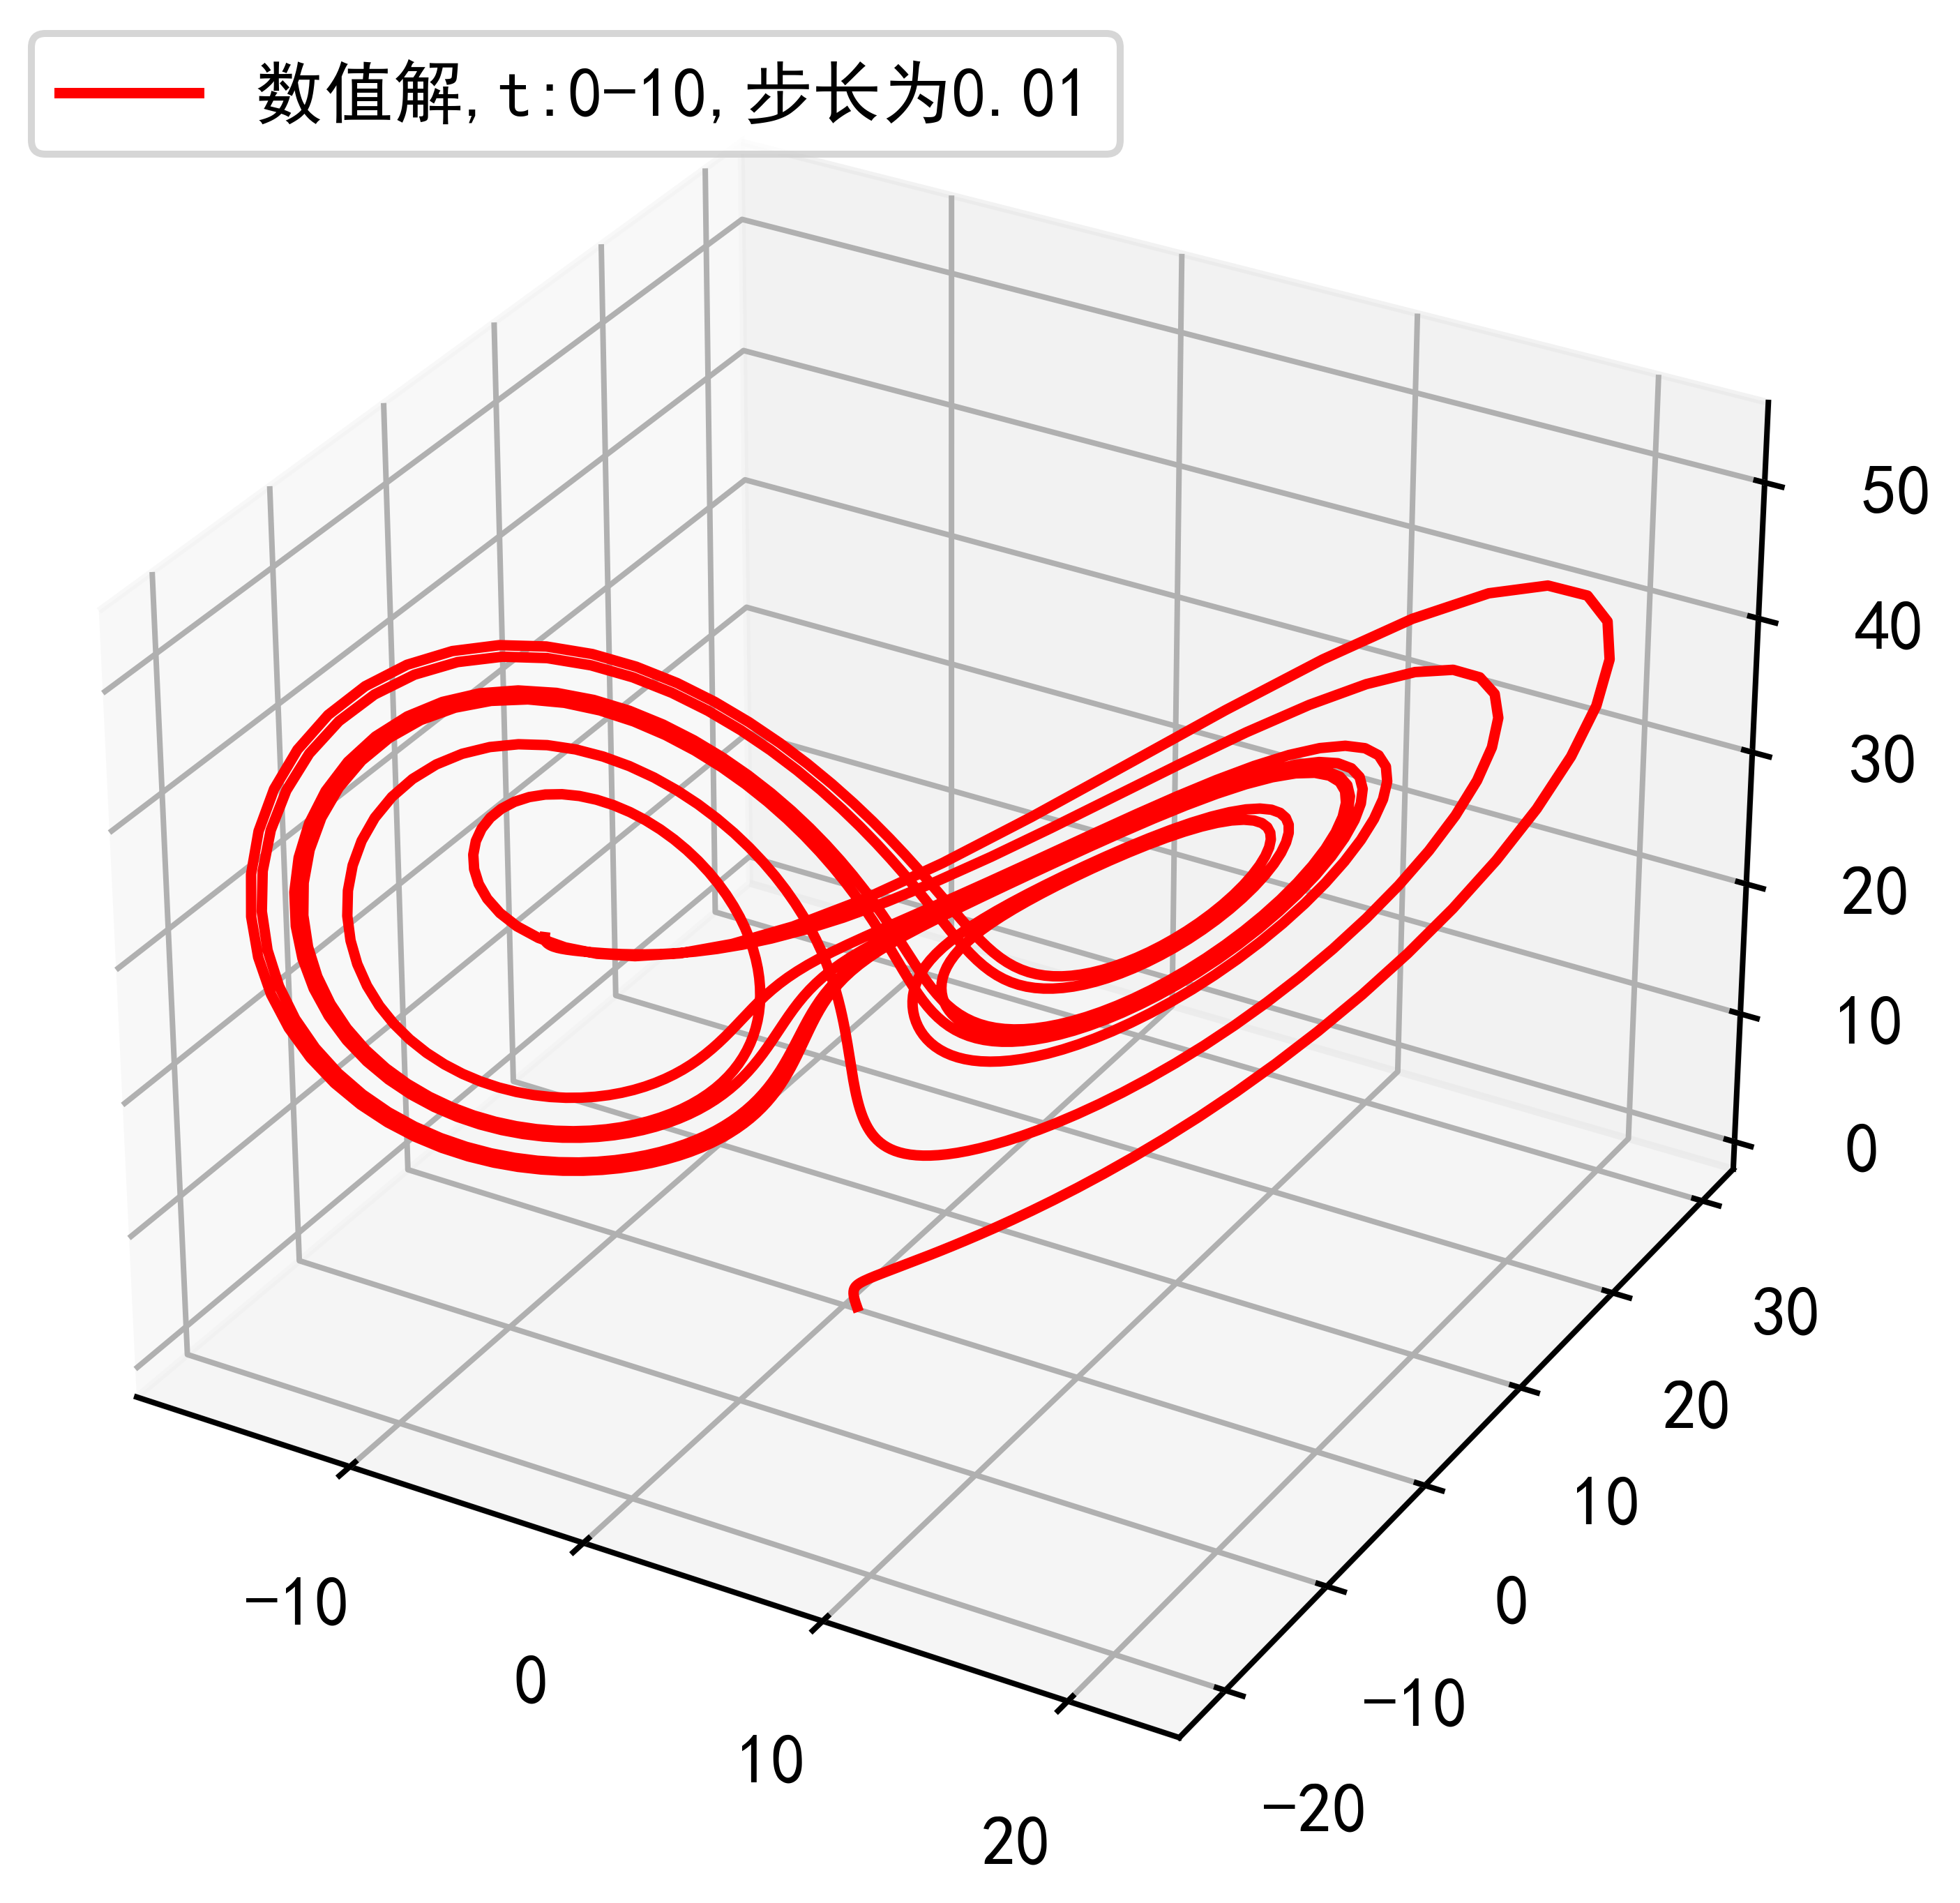
\includegraphics[scale=0.65]{73}
    \caption{起始点为(1,-1,-1)}
    \end{minipage}
    \begin{minipage}[h]{0.48\linewidth}
    \centering
    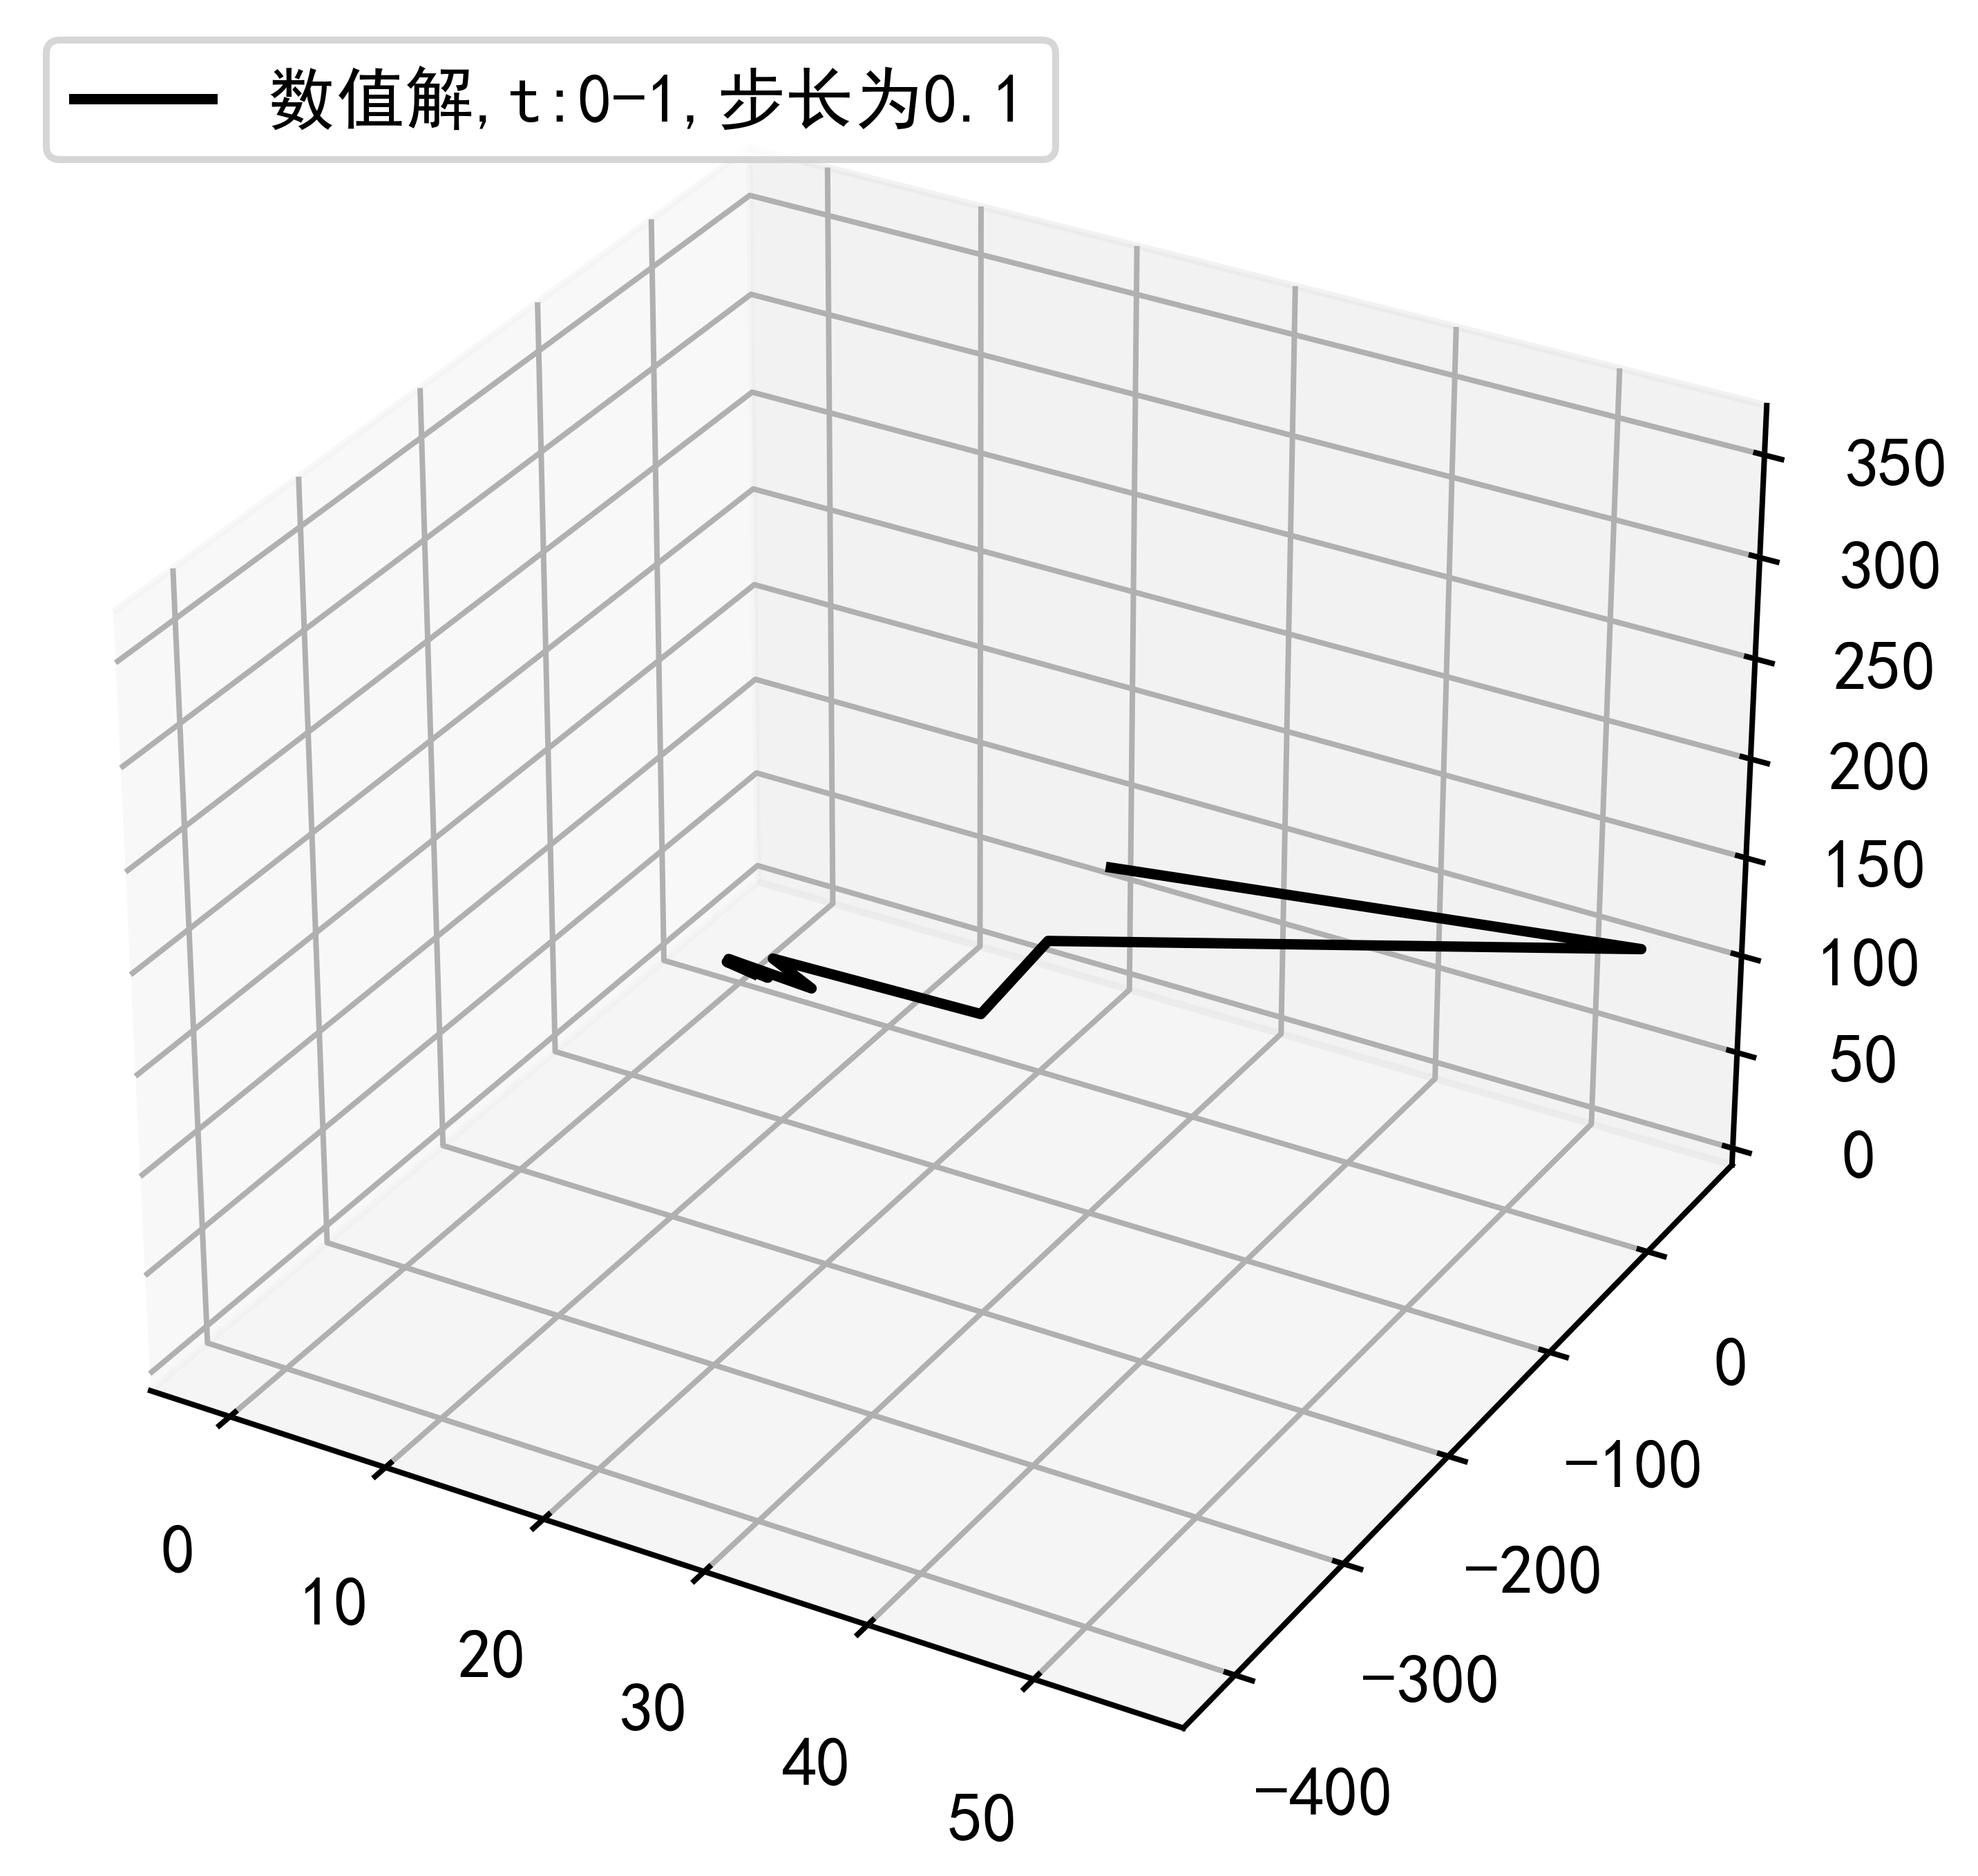
\includegraphics[scale=0.65]{74}
    \caption{起始点为(1,-1,-1)}
    \end{minipage}
\end{figure}
\begin{figure}[H]
    \centering
    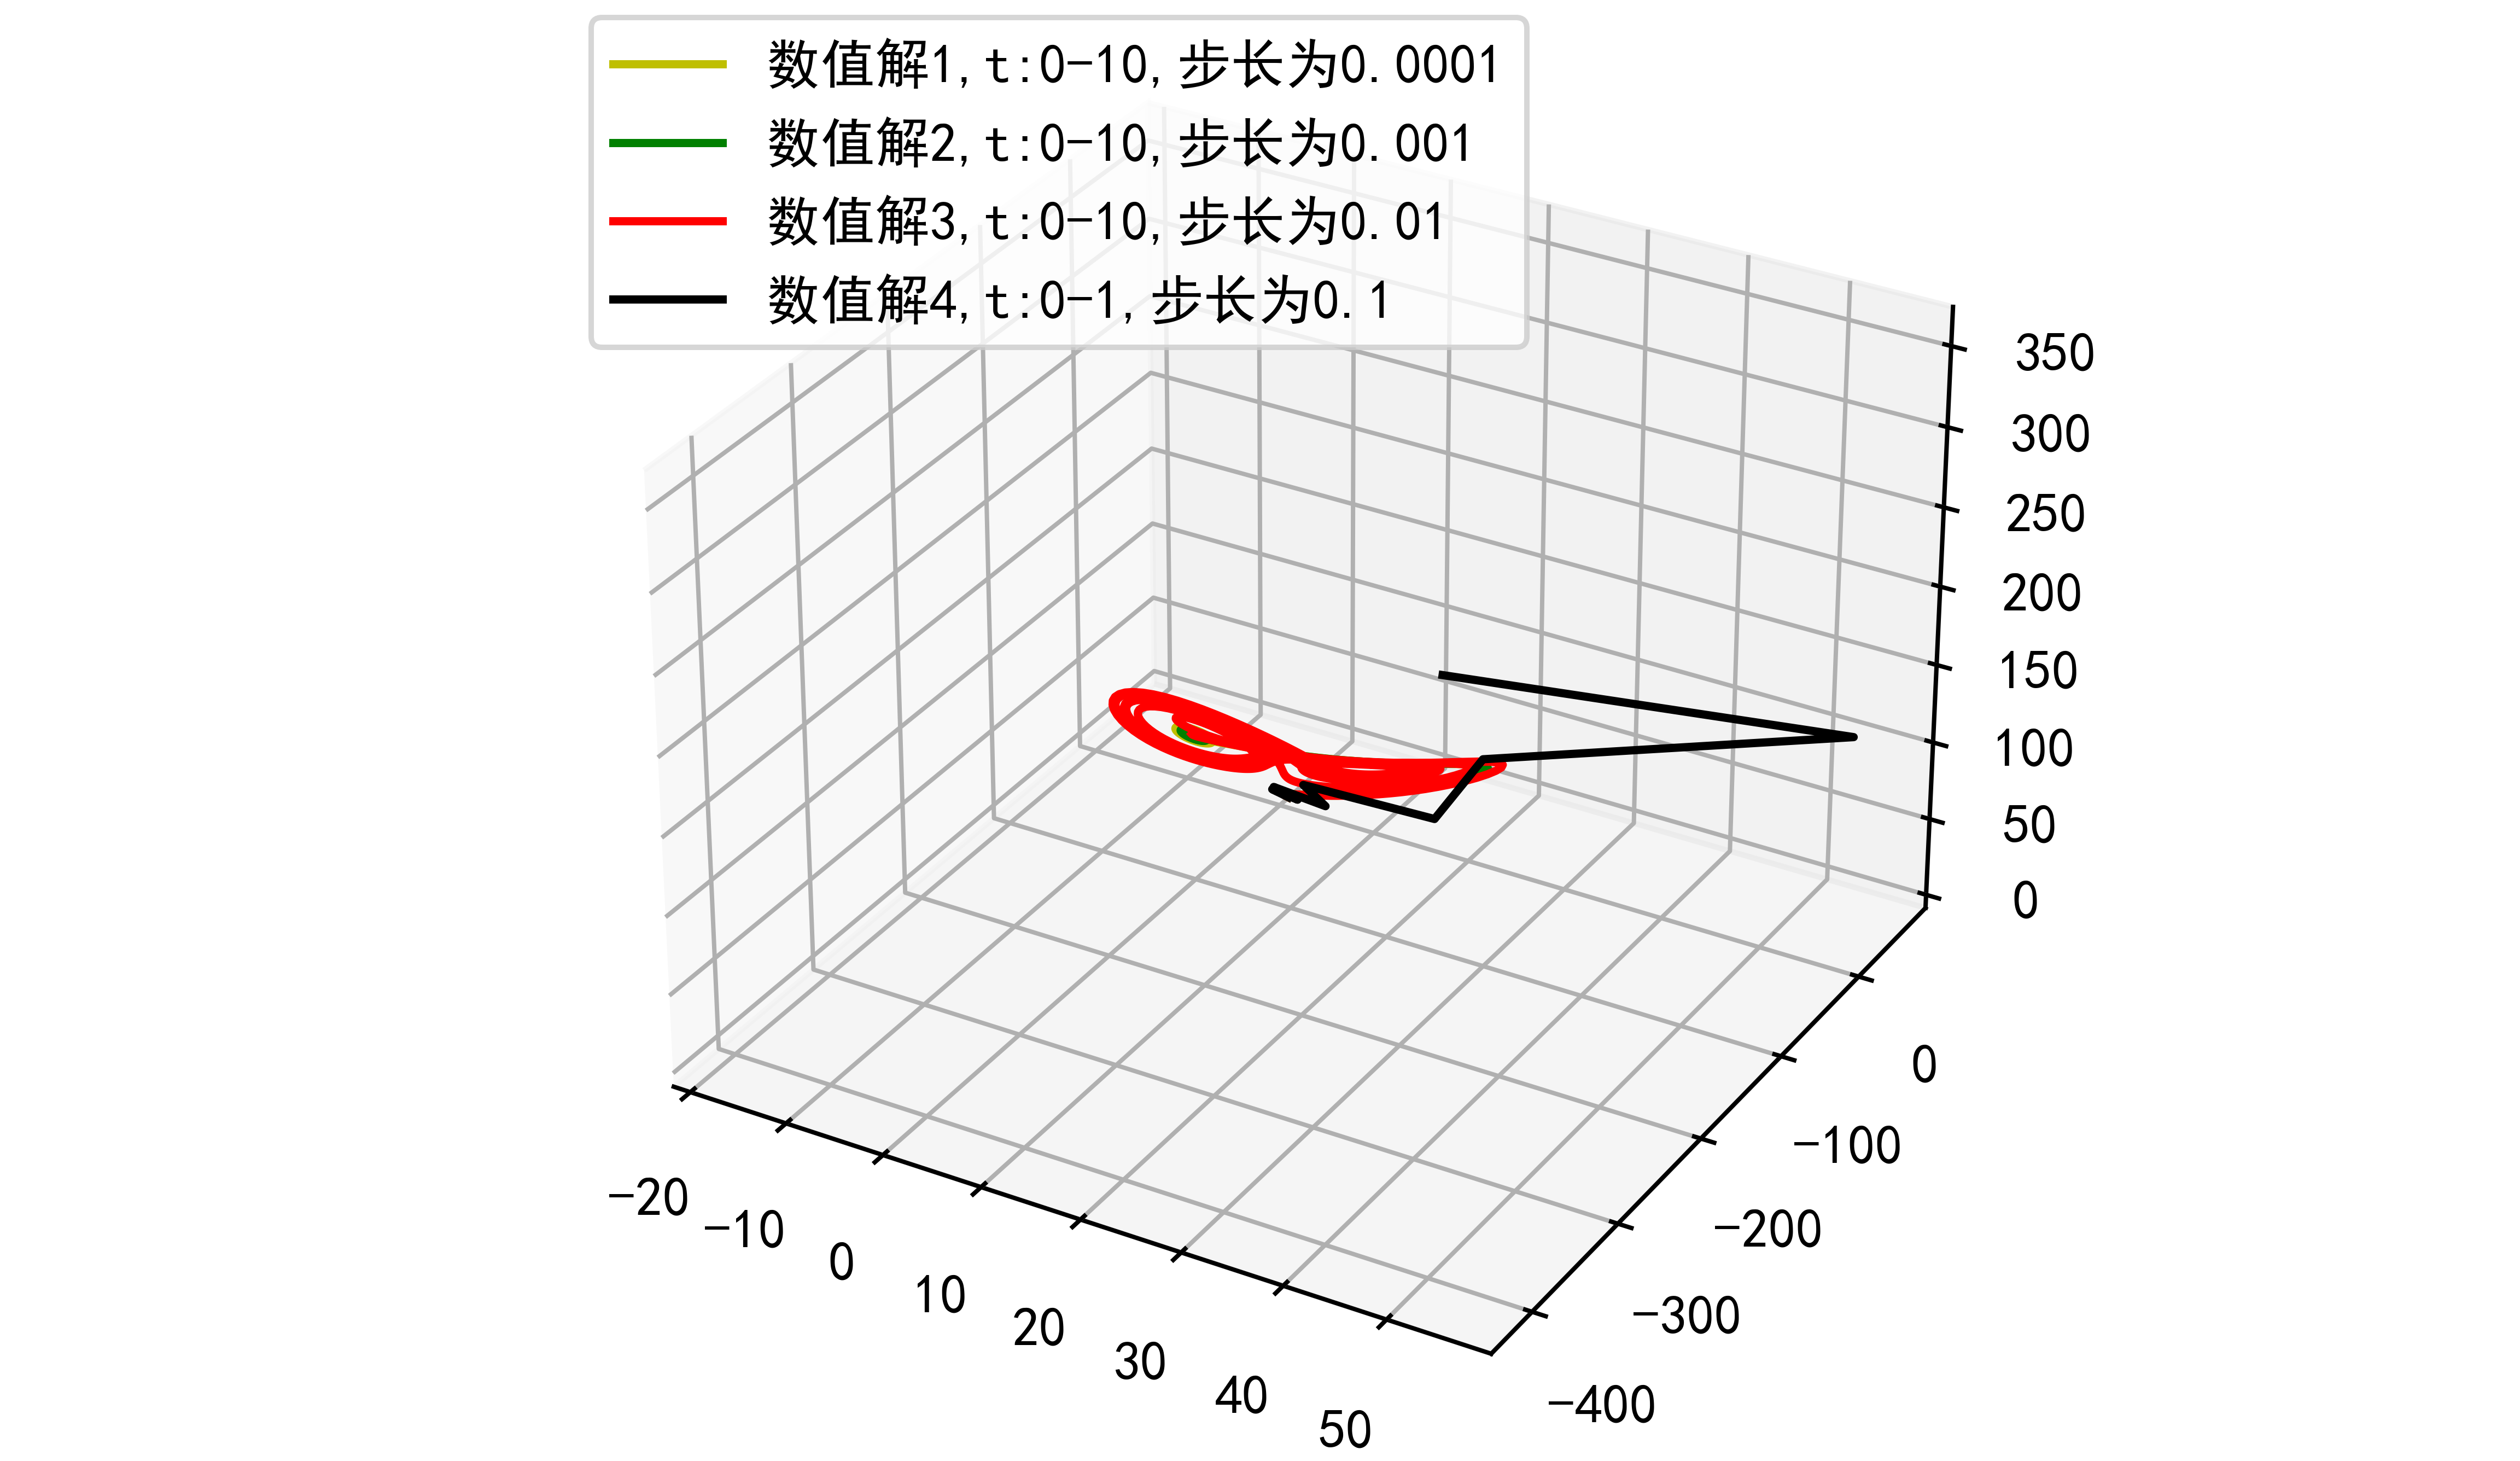
\includegraphics[scale=0.8]{75}
    \caption{起始点为(1,-1,-1)}
\end{figure}

\begin{figure}[h]
    \begin{minipage}{0.48\linewidth}
    \centering
    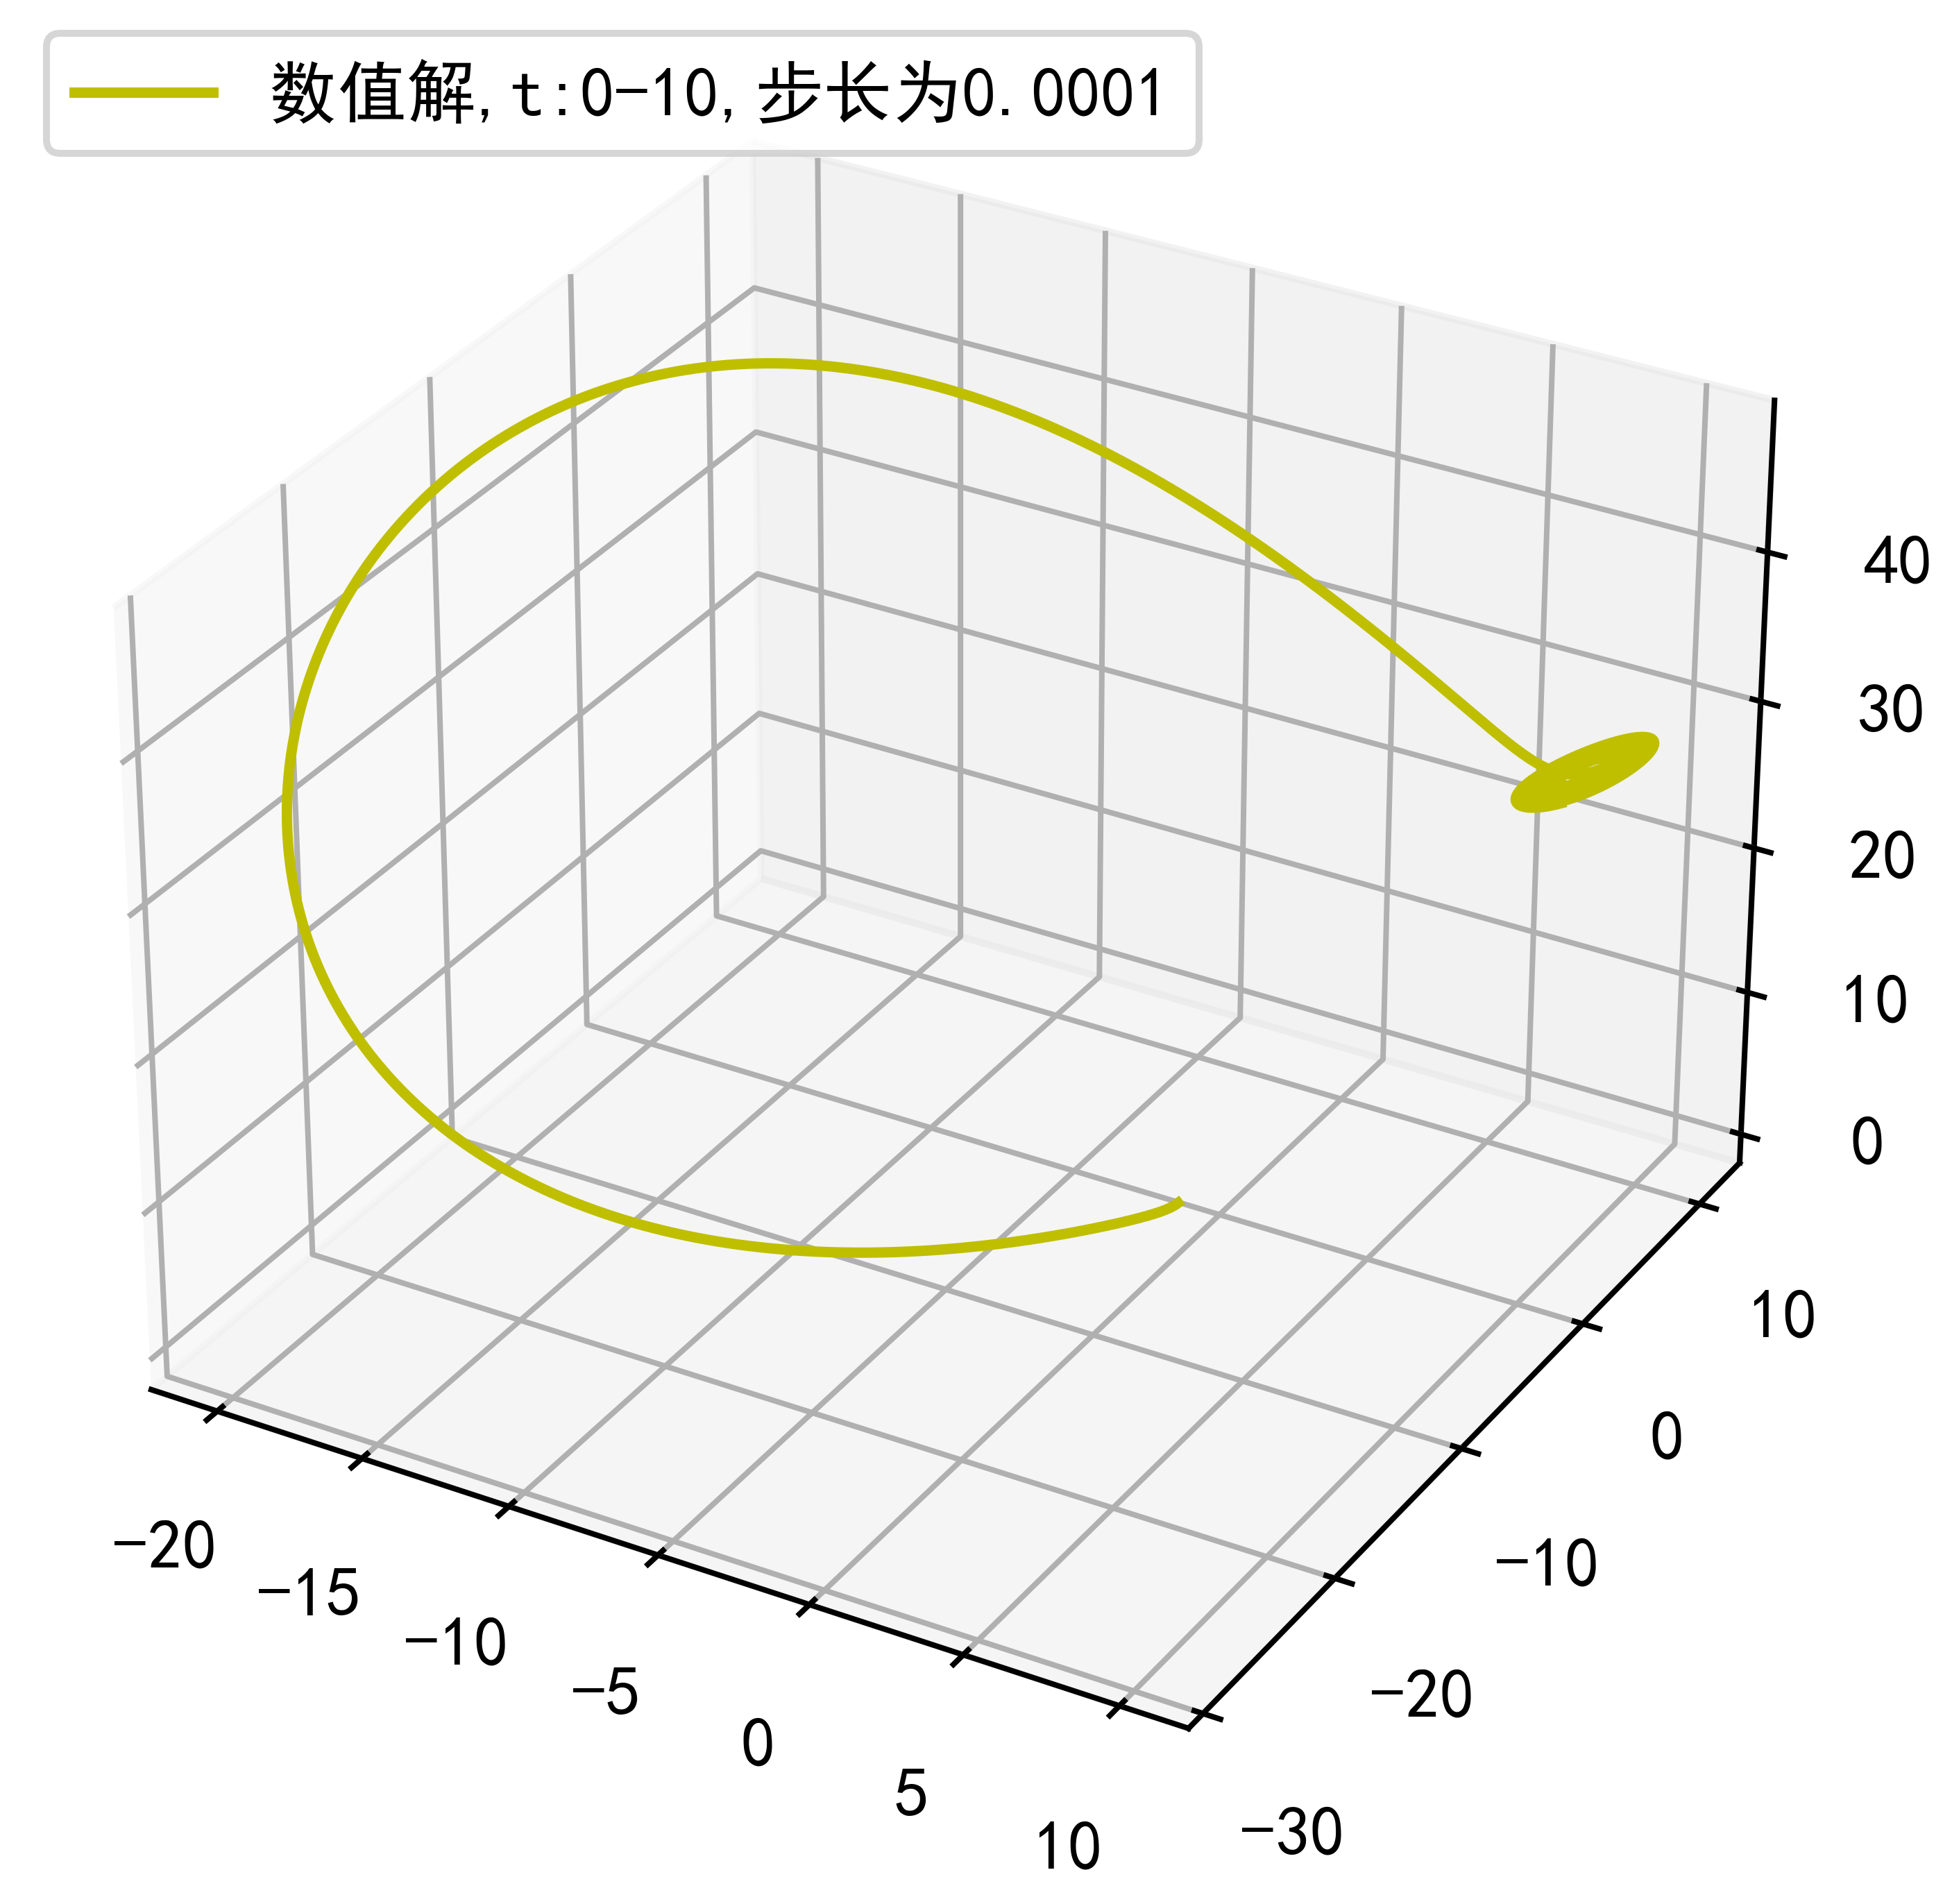
\includegraphics[scale=0.65]{81}
    \caption{起始点为(-1,-1,-1)}
    \end{minipage}
    \begin{minipage}{0.48\linewidth}
    \centering
    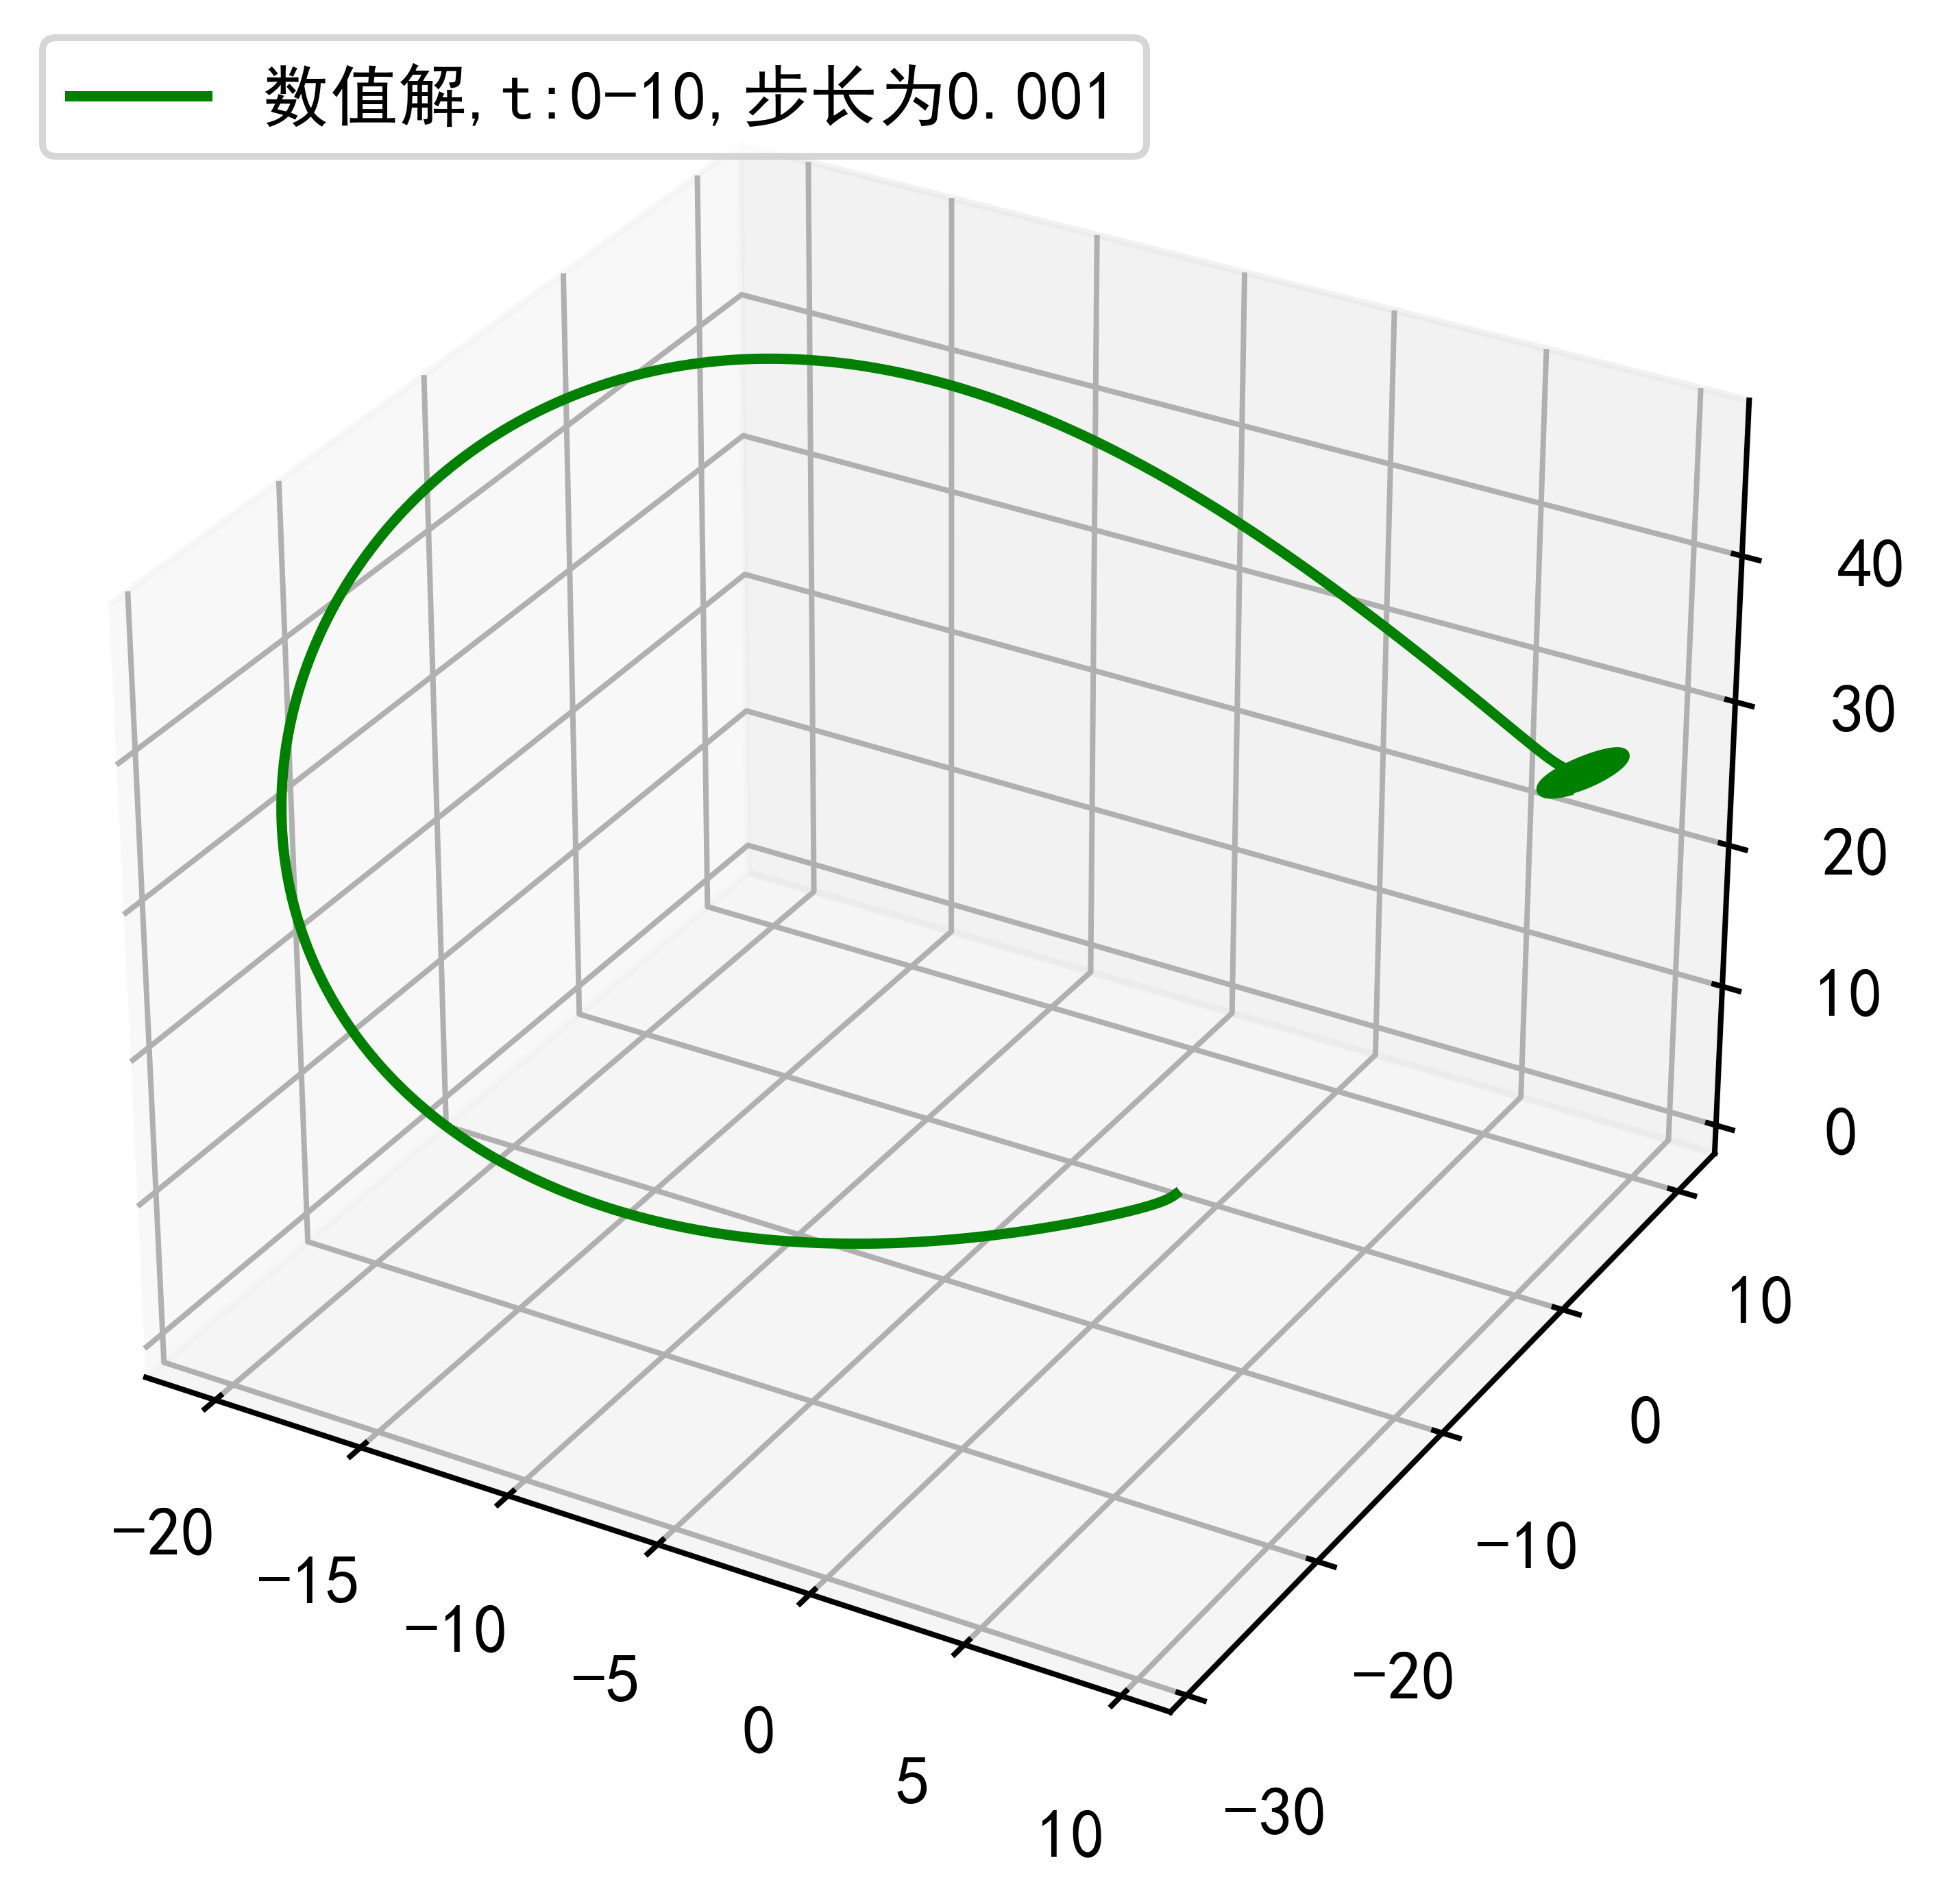
\includegraphics[scale=0.65]{82}
    \caption{起始点为(-1,-1,-1)}
    \end{minipage}
\end{figure}
\begin{figure}[h]
    \begin{minipage}[h]{0.48\linewidth}
    \centering
    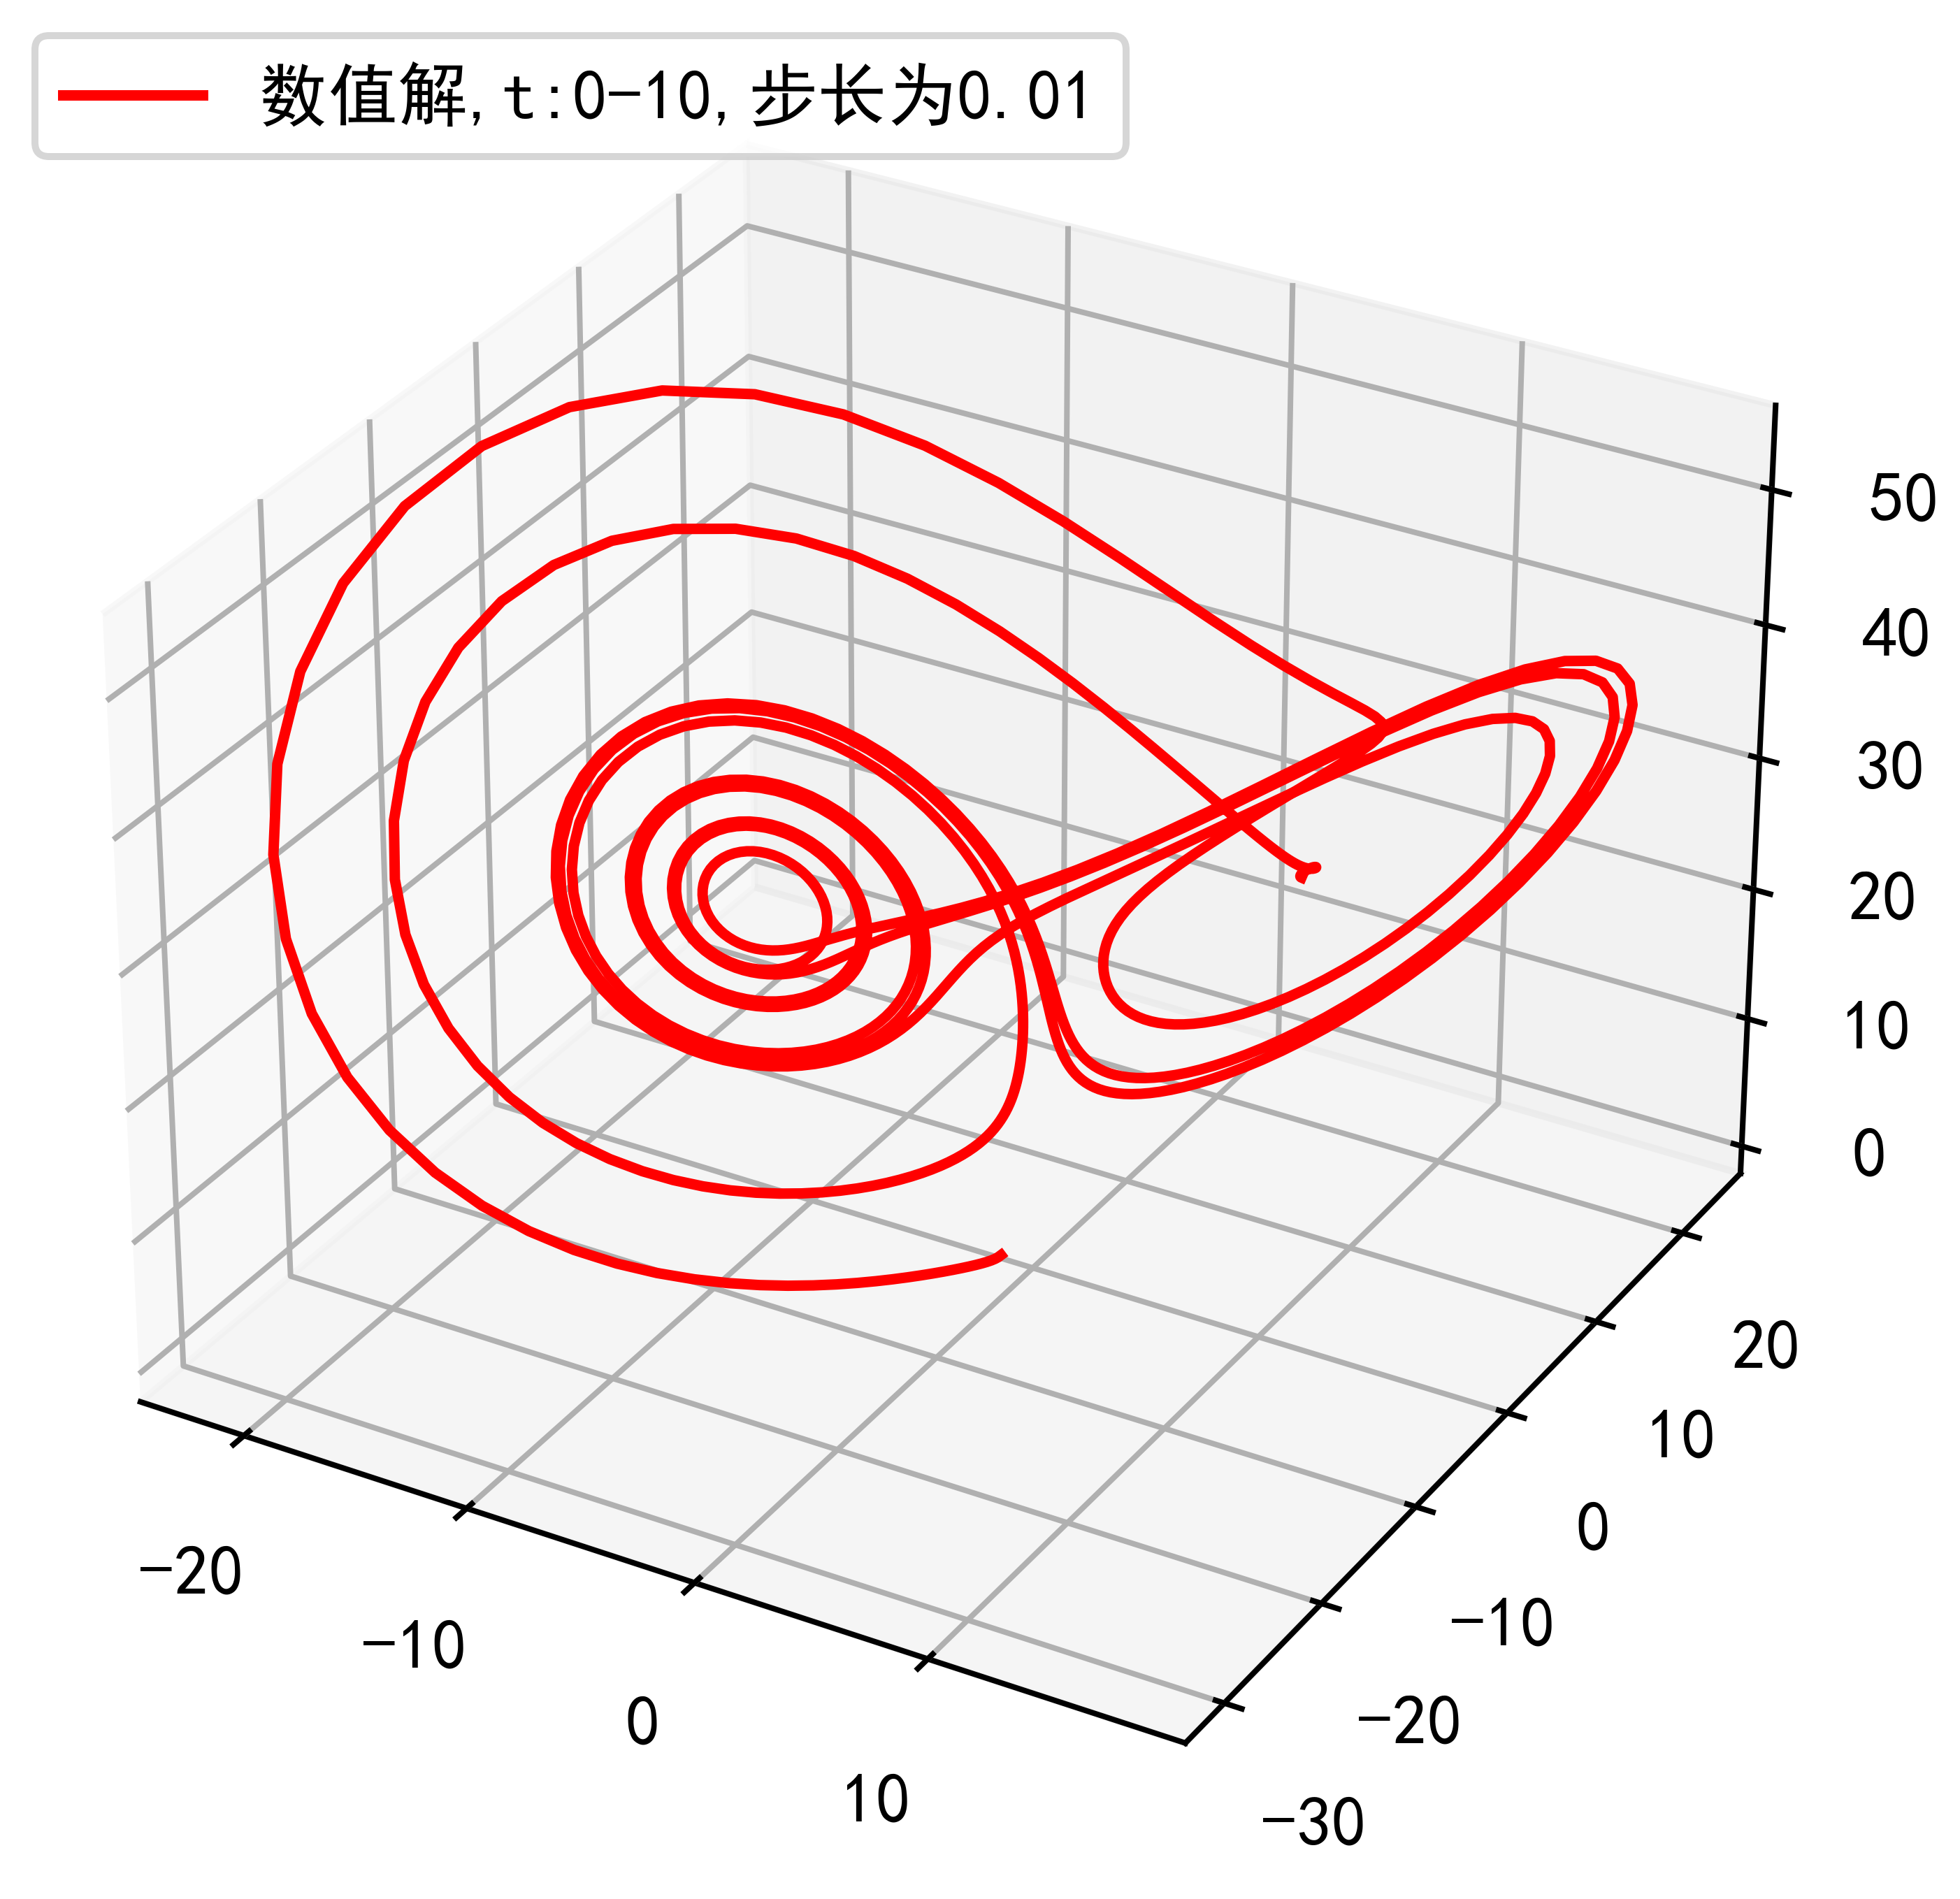
\includegraphics[scale=0.65]{83}
    \caption{起始点为(-1,-1,-1)}
    \end{minipage}
    \begin{minipage}[h]{0.48\linewidth}
    \centering
    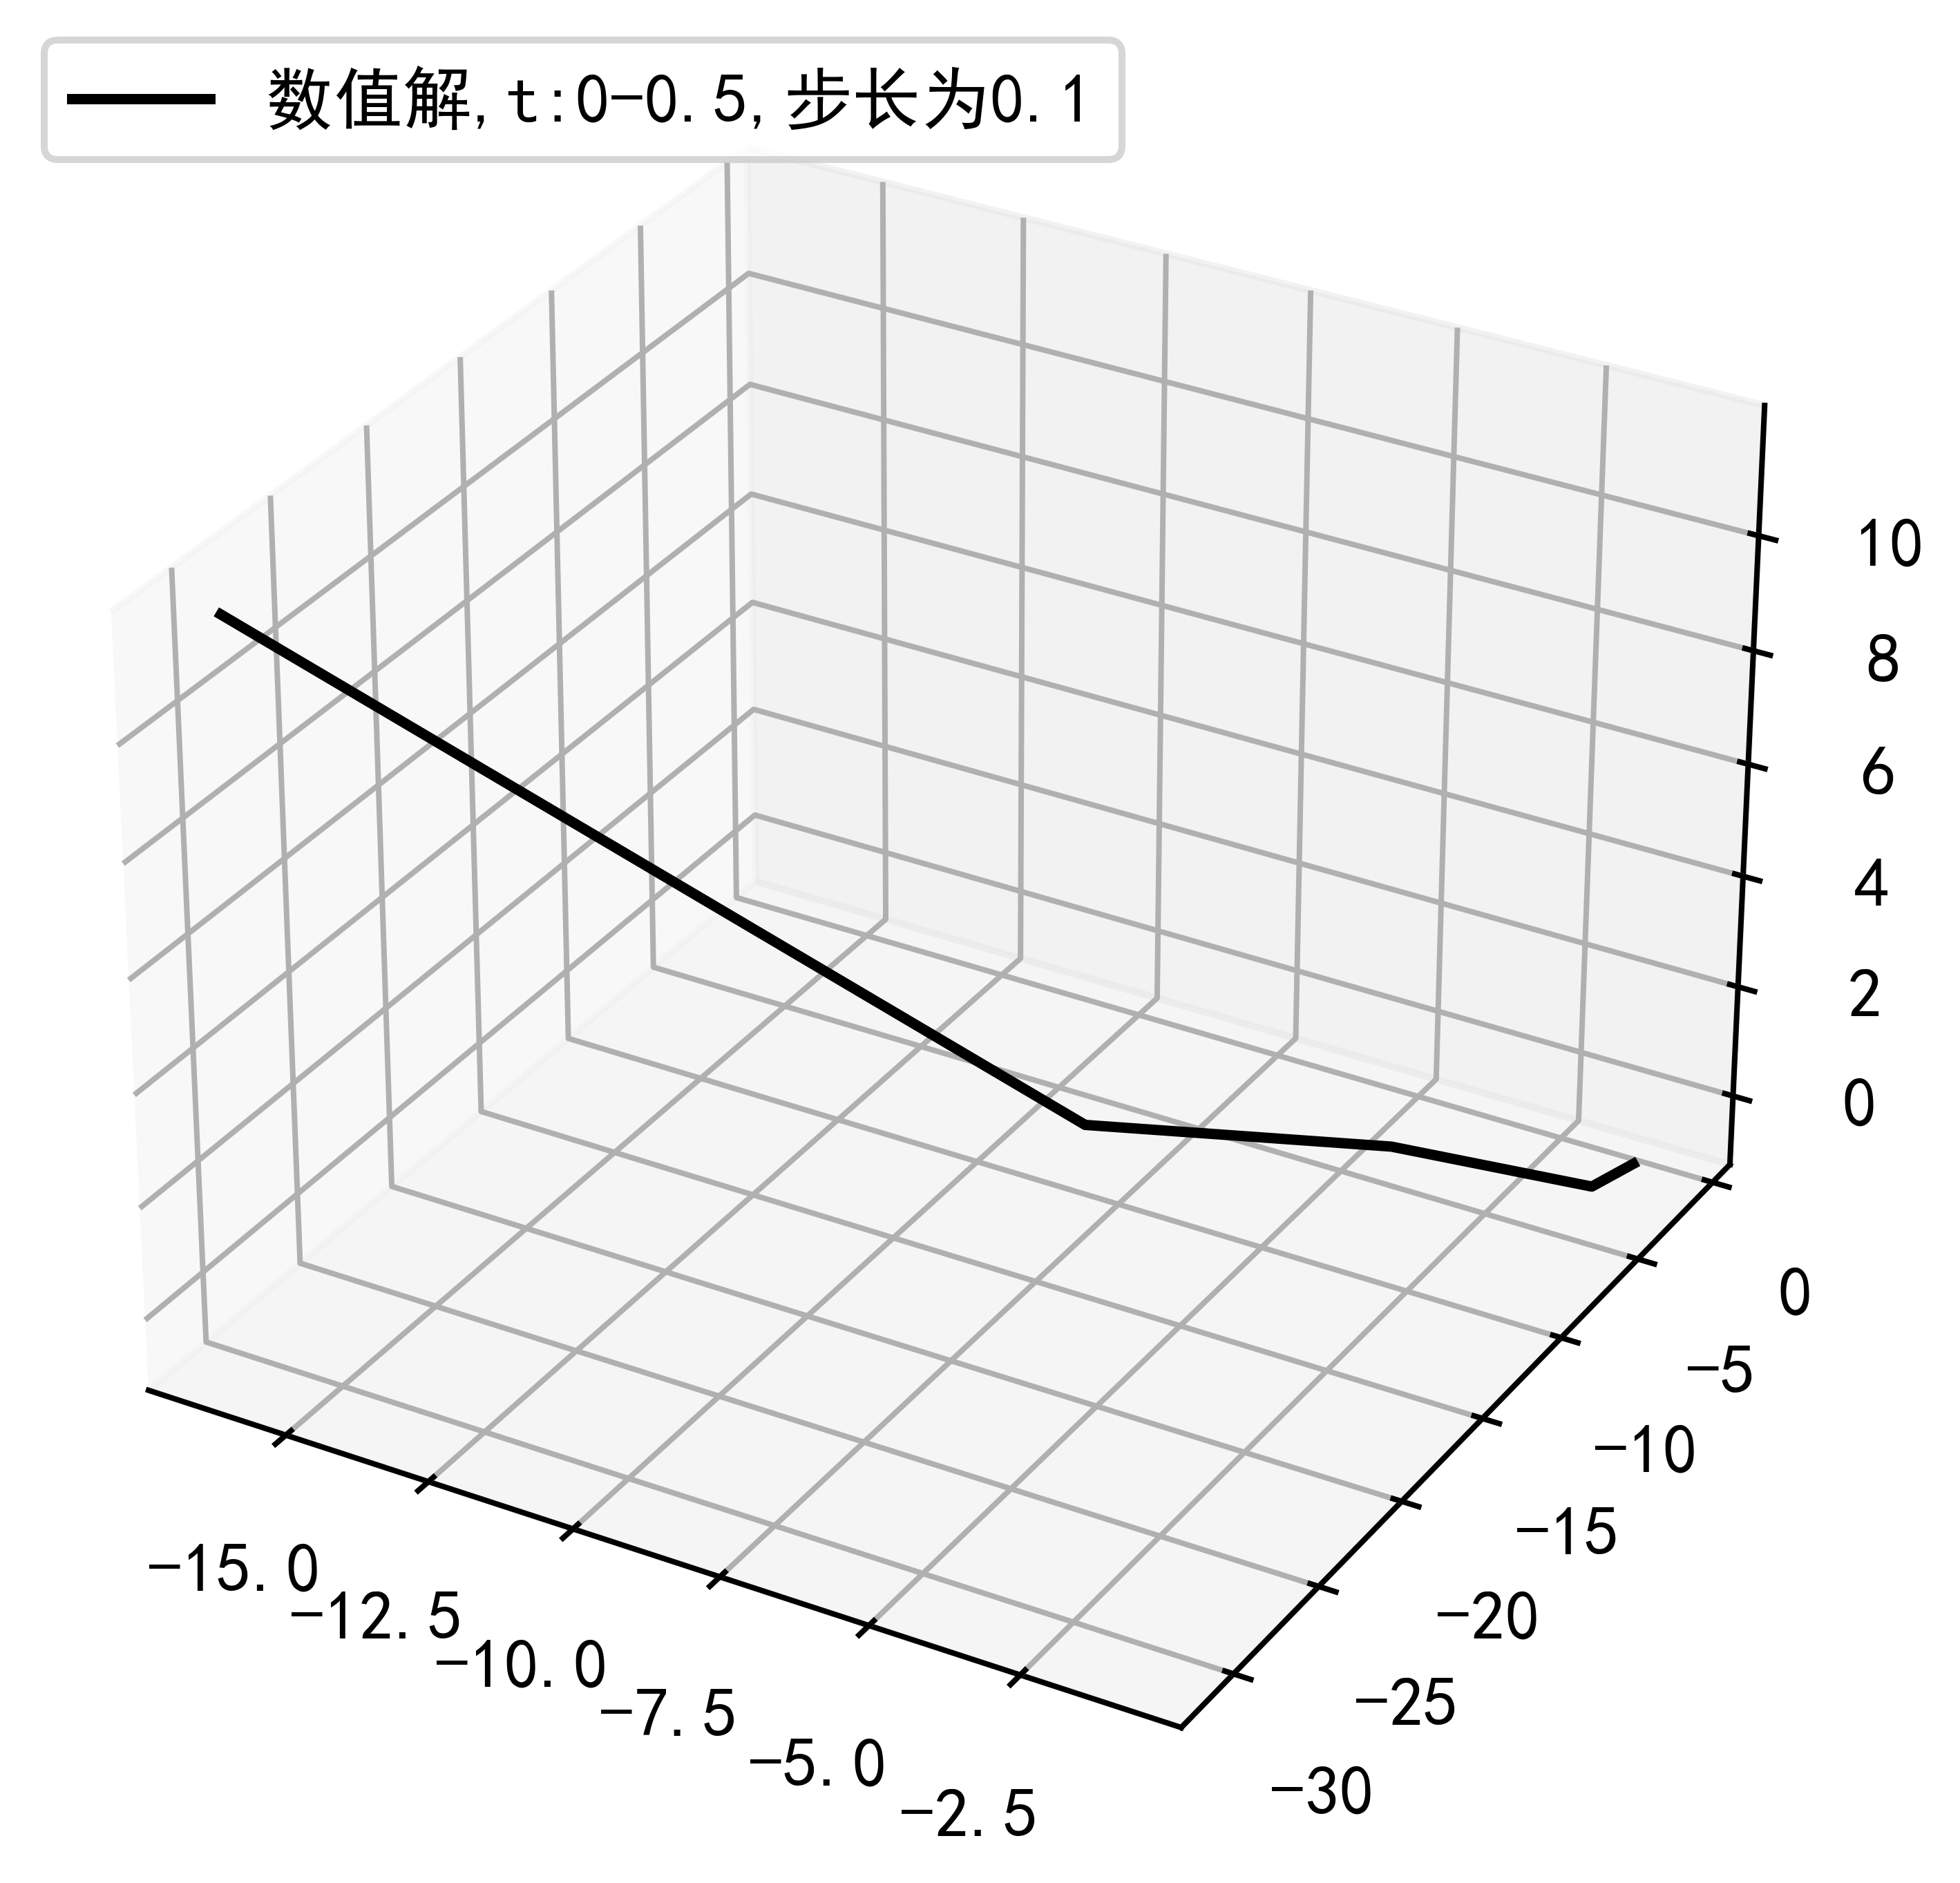
\includegraphics[scale=0.65]{84}
    \caption{起始点为(-1,-1,-1)}
    \end{minipage}
\end{figure}
\begin{figure}[H]
    \centering
    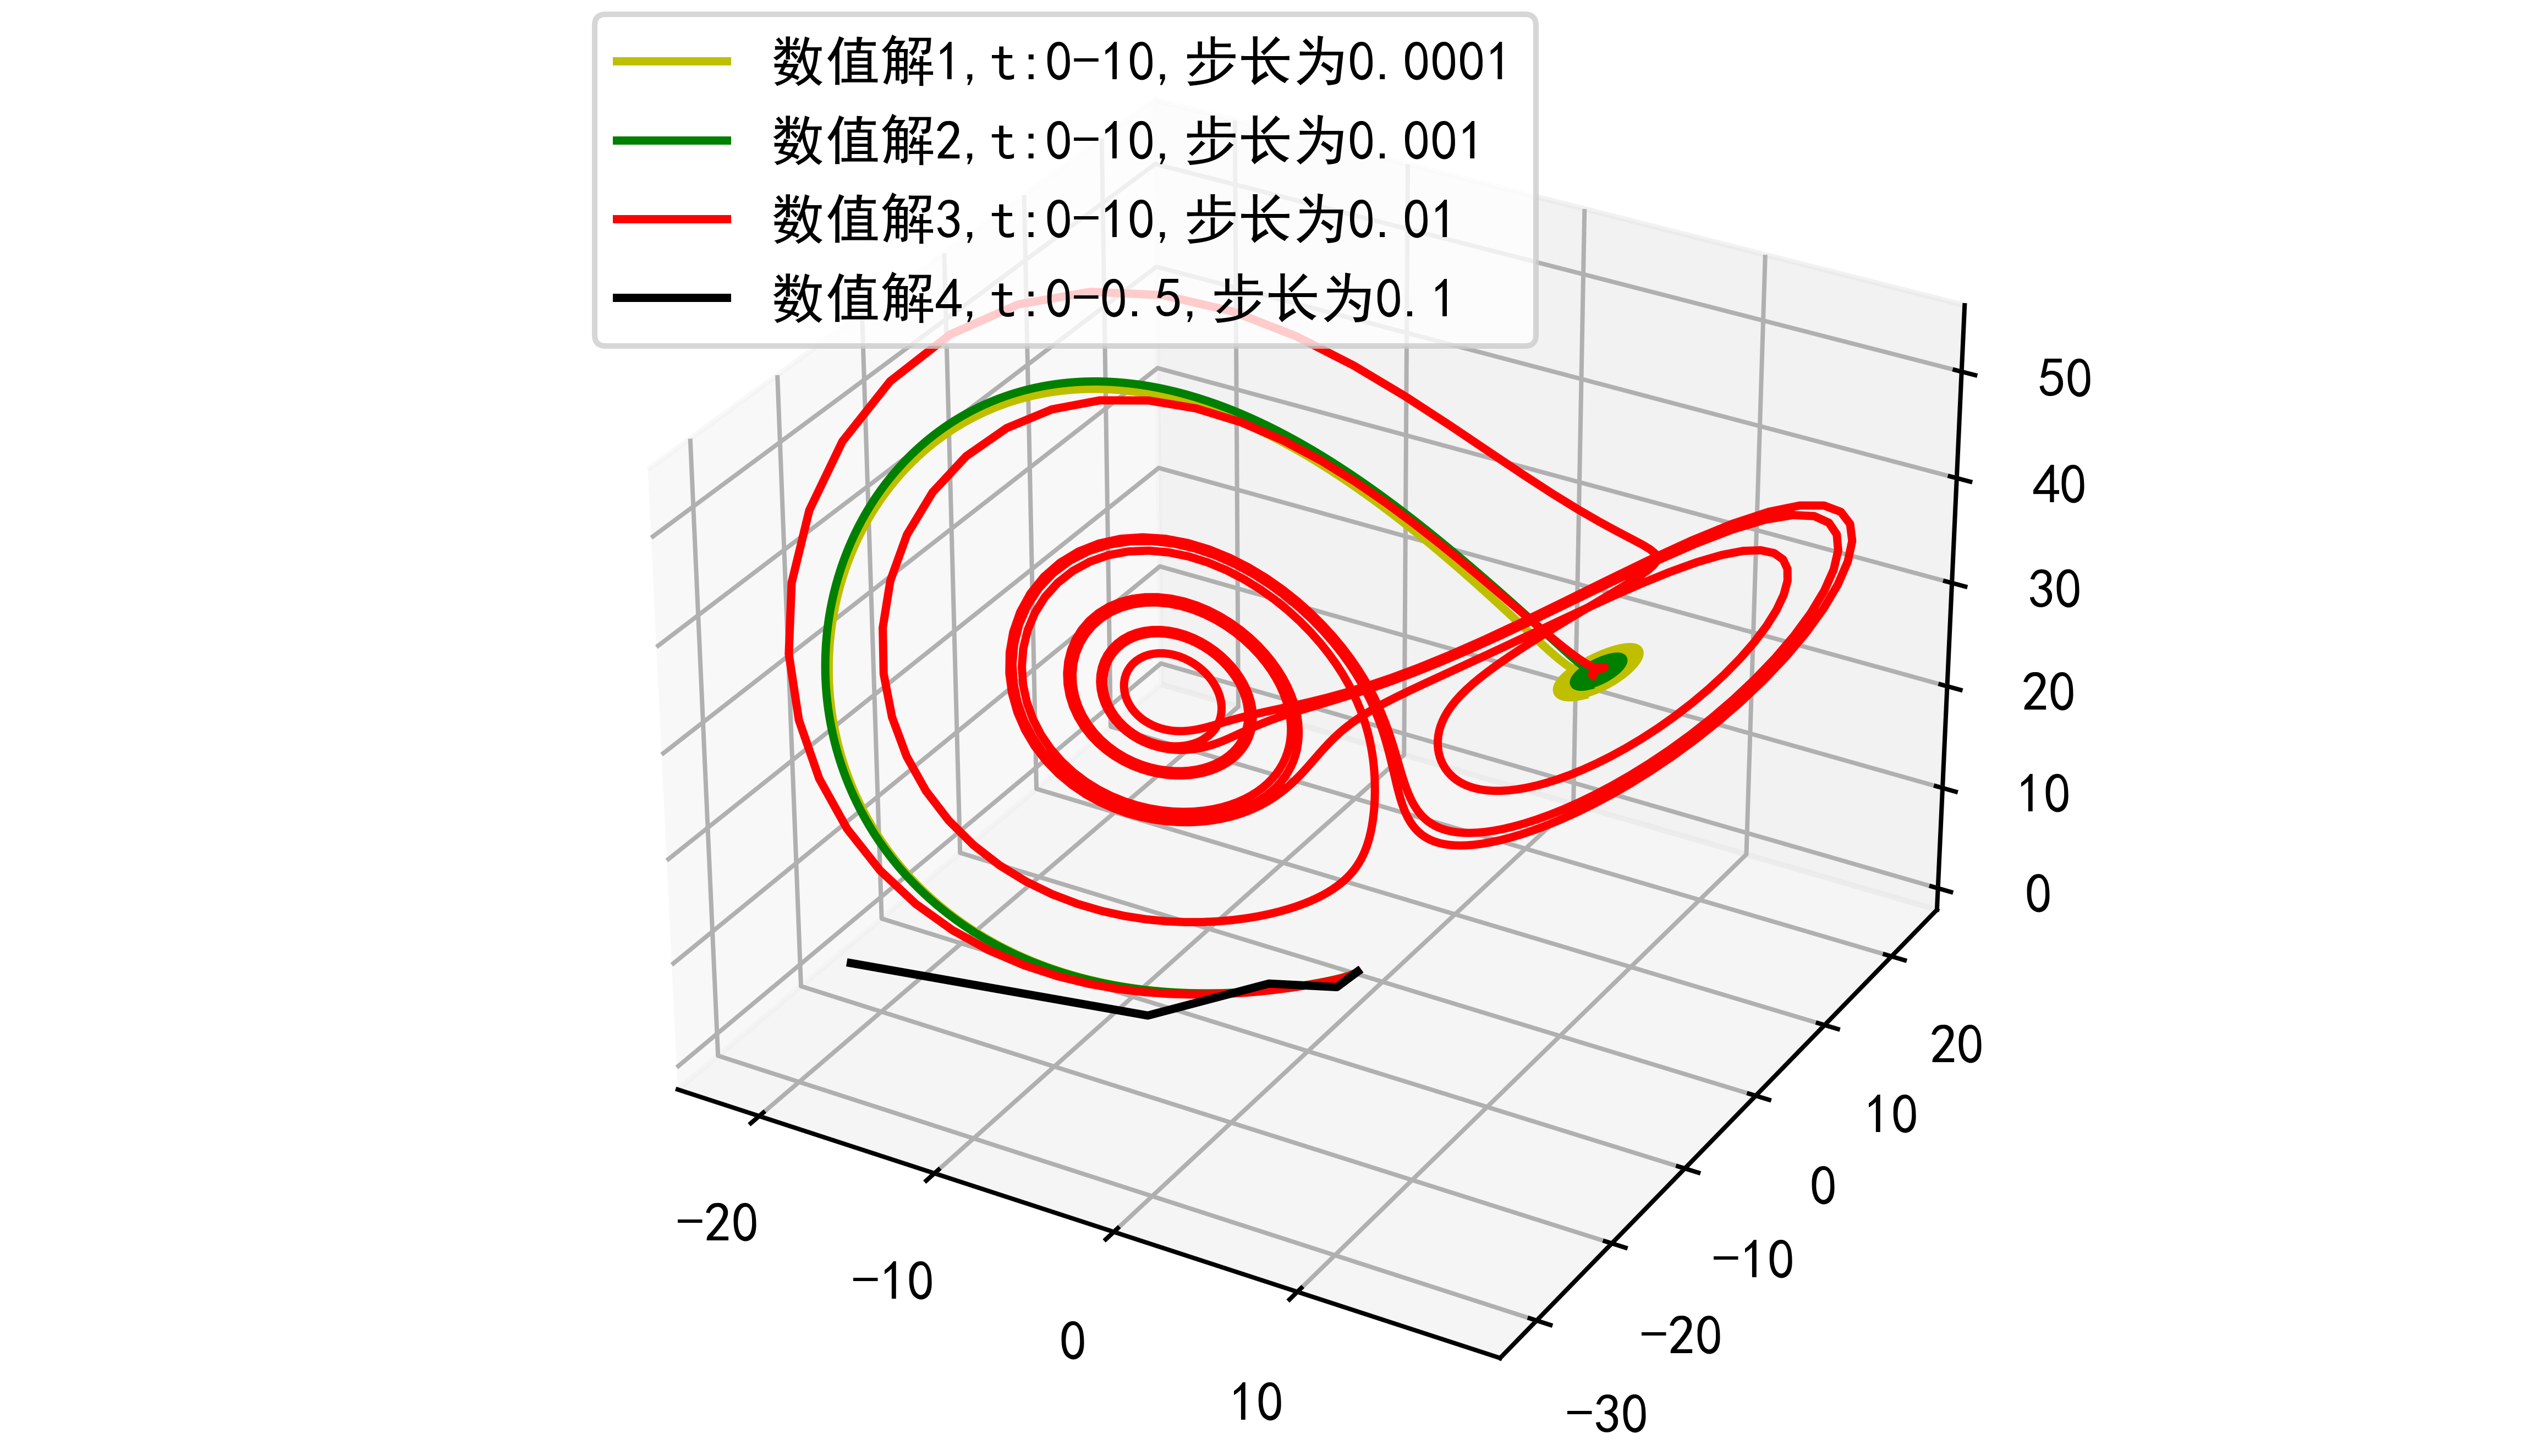
\includegraphics[scale=0.8]{85}
    \caption{起始点为(-1,-1,-1)}
\end{figure}
从以上图像可以看出,如果在求微分方程(组)的数值解时所取步长过大,得到的数值解的行为特征会与真正的行为特征相差甚远.当所取步长足够小时,数值解的行为特征基本稳定,可以近似为原微分方程(组)的解.  
\nocite{*}
\bibliography{Task3}
\end{document}
